\documentclass[aspectratio=169, xcolor={svgnames}]{beamer}
\title{INTERNODES in contact mechanics}
\date{\today}
\author{Bruno Ploumhans \& Fabio Matti}

\usepackage{beamertheme}
\usepackage{listings}
\usepackage{tikz}
\usepackage{pdfpages}
\usepackage{pgfplots}
\pgfplotsset{compat=newest}

%% Nice looking inline code (`ci` stands for code inline)
% Thanks to Stack Overflow
% https://tex.stackexchange.com/questions/140166/making-inline-code-printing-pretty
\newcommand{\ci}[1]{%
  \tikz[baseline=(s.base)]{
    \node(s)[rounded corners,fill=orange!20,draw=gray]{\texttt{#1}};
  }%
}

\lstset{
  basicstyle=\footnotesize,        % the size of the fonts that are used for the code
}

\begin{document}

\begin{frame}[noframenumbering]

    \titlepage

\end{frame}

\begin{frame}{Outline}
    \begin{itemize}
        \item Recap of INTERNODES method
        \item Test cases and results
        \item Implementation discussion
    \end{itemize}
\end{frame}

\begin{frame}{Contact mechanics problems}
\centering
    \begin{tikzpicture}
    \draw[ultra thick, darkblue, fill=darkblue!10!white] (-5, -3) to (5, -3) to (5, 0) to (3, 0) to[out=180,in=0] (0, -0.75) to[out=180,in=0] (-3, 0) to  (-5, 0) -- cycle;
    \draw[ultra thick, darkblue, fill=darkblue!10!white] (3, 2.25) arc(360:180:3) -- cycle;
    %\draw[ultra thick, postaction={-,draw=mainorange,dash pattern=on 0cm off 1.4cm on 2cm}] (3, 0) to[out=180,in=0] (0, -0.75) to[out=180,in=0] (-3, 0);
    \draw[ultra thick, darkblue, dashed] (3, 3) arc(360:180:3) -- cycle;
    \draw[ultra thick, darkblue, dashed] (3, 0) -- (-3, 0);
    \draw[<->, thick] (3.25, 3) -- (3.25, 2.25) node[midway, right] {$d$};
    %\draw[->, thick] (0, 3.75) -- (0, 3.25) node[midway, right] {$F$};
    %\draw[<-, thick] (0.5, -0.8) -- (1.3, -1.4) node[right] {\Large \textcolor{mainblue}{$\Gamma_1$}};
    %\draw[<-, thick] (0.5, -0.6) -- (1.3, 0.4) node[right] {\Large \textcolor{mainblue}{$\Gamma_2$}};
    %\draw[<->, thick] (0, 2.4) -- (2.9, 2.4) node[midway, above] {$R$};
    \node at (0, -2) {\Large \textcolor{mainblue}{$\Omega_1$}};
    \node at (0, 1) {\Large \textcolor{mainblue}{$\Omega_2$}};
\end{tikzpicture}
\end{frame}

\begin{frame}{Radial basis interpolation}
\begin{columns}
\begin{column}{0.5\textwidth}
    \onslide<1->{\flushleft
    Radial basis interpolant of $g : \mathbb{R}^d \to \mathbb{R}$:
    \begin{equation}
        \Pi(\mathbf{x}) = \sum_{m=1}^M g(\boldsymbol{\xi}_m) \phi(\left\| \mathbf{x} -  \boldsymbol{\xi}_m \right\|, r_m)
    \end{equation}
    \begin{itemize}
        \item Radial basis function $\phi$
        \item Interpolation nodes $\boldsymbol{\xi}_1, \dots, \boldsymbol{\xi}_M$
        \item Radius parameters $r_1, \dots, r_M$
    \end{itemize}
    }
    \onslide<2->{\flushleft
    Wendland $C^2$ radial basis function
    \begin{equation*}
        \phi(\delta) = (1 - \delta)_{+}^4(1 + 4\delta) 
    \end{equation*}
    with $\delta = \lVert \mathbf{x} - \boldsymbol{\xi}_m \rVert / r$ are well suited
    }
\end{column}
\begin{column}{0.5\textwidth}
    \centering
    \scalebox{0.9}{\begin{tikzpicture}
    \node at (-2, 3) {$\mathbb{R}^d$};
    \shade[inner color=darkblue!80!white, outer color=white] (0, 0) circle (1.1);
    \fill[darkblue] (0, 0) circle (0.1) node[anchor=south] {$\boldsymbol{\xi}_{j}$};
    \shade[inner color=darkblue!80!white, outer color=white] (-2, 1) circle (0.8);
    \fill[darkblue] (-2, 1) circle (0.1) node[anchor=south] {$\boldsymbol{\xi}_{j+1}$};
    \shade[inner color=darkblue!80!white, outer color=white] (1.6, 2.1) circle (1.4);
    \fill[darkblue] (1.6, 2.1) circle (0.1) node[anchor=south] {$\boldsymbol{\xi}_{j-1}$};
    \draw[darkblue, <->] (0.1, 0) to node[midway, below] {$r_j$} (1.1, 0);
    \draw[darkblue, <->] (-1.9, 1) to node[midway, below] {$r_{j+1}$} (-1.2, 1);
    \draw[darkblue, <->] (1.7, 2.1) to node[midway, below] {$r_{j-1}$} (3, 2.1);
\end{tikzpicture}}
    \onslide<2->{%% Creator: Matplotlib, PGF backend
%%
%% To include the figure in your LaTeX document, write
%%   \input{<filename>.pgf}
%%
%% Make sure the required packages are loaded in your preamble
%%   \usepackage{pgf}
%%
%% Also ensure that all the required font packages are loaded; for instance,
%% the lmodern package is sometimes necessary when using math font.
%%   \usepackage{lmodern}
%%
%% Figures using additional raster images can only be included by \input if
%% they are in the same directory as the main LaTeX file. For loading figures
%% from other directories you can use the `import` package
%%   \usepackage{import}
%%
%% and then include the figures with
%%   \import{<path to file>}{<filename>.pgf}
%%
%% Matplotlib used the following preamble
%%   \usepackage{fontspec}
%%   \setmainfont{DejaVuSans.ttf}[Path=\detokenize{C:/Users/fabio/anaconda3/Lib/site-packages/matplotlib/mpl-data/fonts/ttf/}]
%%   \setsansfont{DejaVuSans.ttf}[Path=\detokenize{C:/Users/fabio/anaconda3/Lib/site-packages/matplotlib/mpl-data/fonts/ttf/}]
%%   \setmonofont{DejaVuSansMono.ttf}[Path=\detokenize{C:/Users/fabio/anaconda3/Lib/site-packages/matplotlib/mpl-data/fonts/ttf/}]
%%
\begingroup%
\makeatletter%
\begin{pgfpicture}%
\pgfpathrectangle{\pgfpointorigin}{\pgfqpoint{2.518403in}{1.425571in}}%
\pgfusepath{use as bounding box, clip}%
\begin{pgfscope}%
\pgfsetbuttcap%
\pgfsetmiterjoin%
\pgfsetlinewidth{0.000000pt}%
\definecolor{currentstroke}{rgb}{1.000000,1.000000,1.000000}%
\pgfsetstrokecolor{currentstroke}%
\pgfsetstrokeopacity{0.000000}%
\pgfsetdash{}{0pt}%
\pgfpathmoveto{\pgfqpoint{-0.000000in}{0.000000in}}%
\pgfpathlineto{\pgfqpoint{2.518403in}{0.000000in}}%
\pgfpathlineto{\pgfqpoint{2.518403in}{1.425571in}}%
\pgfpathlineto{\pgfqpoint{-0.000000in}{1.425571in}}%
\pgfpathlineto{\pgfqpoint{-0.000000in}{0.000000in}}%
\pgfpathclose%
\pgfusepath{}%
\end{pgfscope}%
\begin{pgfscope}%
\pgfsetbuttcap%
\pgfsetmiterjoin%
\definecolor{currentfill}{rgb}{1.000000,1.000000,1.000000}%
\pgfsetfillcolor{currentfill}%
\pgfsetlinewidth{0.000000pt}%
\definecolor{currentstroke}{rgb}{0.000000,0.000000,0.000000}%
\pgfsetstrokecolor{currentstroke}%
\pgfsetstrokeopacity{0.000000}%
\pgfsetdash{}{0pt}%
\pgfpathmoveto{\pgfqpoint{0.480903in}{0.548486in}}%
\pgfpathlineto{\pgfqpoint{2.418403in}{0.548486in}}%
\pgfpathlineto{\pgfqpoint{2.418403in}{1.303486in}}%
\pgfpathlineto{\pgfqpoint{0.480903in}{1.303486in}}%
\pgfpathlineto{\pgfqpoint{0.480903in}{0.548486in}}%
\pgfpathclose%
\pgfusepath{fill}%
\end{pgfscope}%
\begin{pgfscope}%
\pgfsetbuttcap%
\pgfsetroundjoin%
\definecolor{currentfill}{rgb}{0.000000,0.000000,0.000000}%
\pgfsetfillcolor{currentfill}%
\pgfsetlinewidth{0.803000pt}%
\definecolor{currentstroke}{rgb}{0.000000,0.000000,0.000000}%
\pgfsetstrokecolor{currentstroke}%
\pgfsetdash{}{0pt}%
\pgfsys@defobject{currentmarker}{\pgfqpoint{0.000000in}{-0.048611in}}{\pgfqpoint{0.000000in}{0.000000in}}{%
\pgfpathmoveto{\pgfqpoint{0.000000in}{0.000000in}}%
\pgfpathlineto{\pgfqpoint{0.000000in}{-0.048611in}}%
\pgfusepath{stroke,fill}%
}%
\begin{pgfscope}%
\pgfsys@transformshift{0.480903in}{0.548486in}%
\pgfsys@useobject{currentmarker}{}%
\end{pgfscope}%
\end{pgfscope}%
\begin{pgfscope}%
\definecolor{textcolor}{rgb}{0.000000,0.000000,0.000000}%
\pgfsetstrokecolor{textcolor}%
\pgfsetfillcolor{textcolor}%
\pgftext[x=0.480903in,y=0.451264in,,top]{\color{textcolor}\rmfamily\fontsize{11.000000}{13.200000}\selectfont \(\displaystyle {0.0}\)}%
\end{pgfscope}%
\begin{pgfscope}%
\pgfsetbuttcap%
\pgfsetroundjoin%
\definecolor{currentfill}{rgb}{0.000000,0.000000,0.000000}%
\pgfsetfillcolor{currentfill}%
\pgfsetlinewidth{0.803000pt}%
\definecolor{currentstroke}{rgb}{0.000000,0.000000,0.000000}%
\pgfsetstrokecolor{currentstroke}%
\pgfsetdash{}{0pt}%
\pgfsys@defobject{currentmarker}{\pgfqpoint{0.000000in}{-0.048611in}}{\pgfqpoint{0.000000in}{0.000000in}}{%
\pgfpathmoveto{\pgfqpoint{0.000000in}{0.000000in}}%
\pgfpathlineto{\pgfqpoint{0.000000in}{-0.048611in}}%
\pgfusepath{stroke,fill}%
}%
\begin{pgfscope}%
\pgfsys@transformshift{1.288194in}{0.548486in}%
\pgfsys@useobject{currentmarker}{}%
\end{pgfscope}%
\end{pgfscope}%
\begin{pgfscope}%
\definecolor{textcolor}{rgb}{0.000000,0.000000,0.000000}%
\pgfsetstrokecolor{textcolor}%
\pgfsetfillcolor{textcolor}%
\pgftext[x=1.288194in,y=0.451264in,,top]{\color{textcolor}\rmfamily\fontsize{11.000000}{13.200000}\selectfont \(\displaystyle {0.5}\)}%
\end{pgfscope}%
\begin{pgfscope}%
\pgfsetbuttcap%
\pgfsetroundjoin%
\definecolor{currentfill}{rgb}{0.000000,0.000000,0.000000}%
\pgfsetfillcolor{currentfill}%
\pgfsetlinewidth{0.803000pt}%
\definecolor{currentstroke}{rgb}{0.000000,0.000000,0.000000}%
\pgfsetstrokecolor{currentstroke}%
\pgfsetdash{}{0pt}%
\pgfsys@defobject{currentmarker}{\pgfqpoint{0.000000in}{-0.048611in}}{\pgfqpoint{0.000000in}{0.000000in}}{%
\pgfpathmoveto{\pgfqpoint{0.000000in}{0.000000in}}%
\pgfpathlineto{\pgfqpoint{0.000000in}{-0.048611in}}%
\pgfusepath{stroke,fill}%
}%
\begin{pgfscope}%
\pgfsys@transformshift{2.095486in}{0.548486in}%
\pgfsys@useobject{currentmarker}{}%
\end{pgfscope}%
\end{pgfscope}%
\begin{pgfscope}%
\definecolor{textcolor}{rgb}{0.000000,0.000000,0.000000}%
\pgfsetstrokecolor{textcolor}%
\pgfsetfillcolor{textcolor}%
\pgftext[x=2.095486in,y=0.451264in,,top]{\color{textcolor}\rmfamily\fontsize{11.000000}{13.200000}\selectfont \(\displaystyle {1.0}\)}%
\end{pgfscope}%
\begin{pgfscope}%
\definecolor{textcolor}{rgb}{0.000000,0.000000,0.000000}%
\pgfsetstrokecolor{textcolor}%
\pgfsetfillcolor{textcolor}%
\pgftext[x=1.449653in,y=0.247854in,,top]{\color{textcolor}\rmfamily\fontsize{11.000000}{13.200000}\selectfont \(\displaystyle \delta\)}%
\end{pgfscope}%
\begin{pgfscope}%
\pgfsetbuttcap%
\pgfsetroundjoin%
\definecolor{currentfill}{rgb}{0.000000,0.000000,0.000000}%
\pgfsetfillcolor{currentfill}%
\pgfsetlinewidth{0.803000pt}%
\definecolor{currentstroke}{rgb}{0.000000,0.000000,0.000000}%
\pgfsetstrokecolor{currentstroke}%
\pgfsetdash{}{0pt}%
\pgfsys@defobject{currentmarker}{\pgfqpoint{-0.048611in}{0.000000in}}{\pgfqpoint{-0.000000in}{0.000000in}}{%
\pgfpathmoveto{\pgfqpoint{-0.000000in}{0.000000in}}%
\pgfpathlineto{\pgfqpoint{-0.048611in}{0.000000in}}%
\pgfusepath{stroke,fill}%
}%
\begin{pgfscope}%
\pgfsys@transformshift{0.480903in}{0.548486in}%
\pgfsys@useobject{currentmarker}{}%
\end{pgfscope}%
\end{pgfscope}%
\begin{pgfscope}%
\definecolor{textcolor}{rgb}{0.000000,0.000000,0.000000}%
\pgfsetstrokecolor{textcolor}%
\pgfsetfillcolor{textcolor}%
\pgftext[x=0.307639in, y=0.490448in, left, base]{\color{textcolor}\rmfamily\fontsize{11.000000}{13.200000}\selectfont \(\displaystyle {0}\)}%
\end{pgfscope}%
\begin{pgfscope}%
\pgfsetbuttcap%
\pgfsetroundjoin%
\definecolor{currentfill}{rgb}{0.000000,0.000000,0.000000}%
\pgfsetfillcolor{currentfill}%
\pgfsetlinewidth{0.803000pt}%
\definecolor{currentstroke}{rgb}{0.000000,0.000000,0.000000}%
\pgfsetstrokecolor{currentstroke}%
\pgfsetdash{}{0pt}%
\pgfsys@defobject{currentmarker}{\pgfqpoint{-0.048611in}{0.000000in}}{\pgfqpoint{-0.000000in}{0.000000in}}{%
\pgfpathmoveto{\pgfqpoint{-0.000000in}{0.000000in}}%
\pgfpathlineto{\pgfqpoint{-0.048611in}{0.000000in}}%
\pgfusepath{stroke,fill}%
}%
\begin{pgfscope}%
\pgfsys@transformshift{0.480903in}{1.267533in}%
\pgfsys@useobject{currentmarker}{}%
\end{pgfscope}%
\end{pgfscope}%
\begin{pgfscope}%
\definecolor{textcolor}{rgb}{0.000000,0.000000,0.000000}%
\pgfsetstrokecolor{textcolor}%
\pgfsetfillcolor{textcolor}%
\pgftext[x=0.307639in, y=1.209496in, left, base]{\color{textcolor}\rmfamily\fontsize{11.000000}{13.200000}\selectfont \(\displaystyle {1}\)}%
\end{pgfscope}%
\begin{pgfscope}%
\definecolor{textcolor}{rgb}{0.000000,0.000000,0.000000}%
\pgfsetstrokecolor{textcolor}%
\pgfsetfillcolor{textcolor}%
\pgftext[x=0.252083in,y=0.925986in,,bottom,rotate=90.000000]{\color{textcolor}\rmfamily\fontsize{11.000000}{13.200000}\selectfont \(\displaystyle \phi(\delta)\)}%
\end{pgfscope}%
\begin{pgfscope}%
\pgfpathrectangle{\pgfqpoint{0.480903in}{0.548486in}}{\pgfqpoint{1.937500in}{0.755000in}}%
\pgfusepath{clip}%
\pgfsetrectcap%
\pgfsetroundjoin%
\pgfsetlinewidth{1.505625pt}%
\definecolor{currentstroke}{rgb}{0.184314,0.270588,0.360784}%
\pgfsetstrokecolor{currentstroke}%
\pgfsetdash{}{0pt}%
\pgfpathmoveto{\pgfqpoint{0.480903in}{1.267533in}}%
\pgfpathlineto{\pgfqpoint{0.500473in}{1.266502in}}%
\pgfpathlineto{\pgfqpoint{0.520044in}{1.263509in}}%
\pgfpathlineto{\pgfqpoint{0.539615in}{1.258698in}}%
\pgfpathlineto{\pgfqpoint{0.559185in}{1.252210in}}%
\pgfpathlineto{\pgfqpoint{0.578756in}{1.244180in}}%
\pgfpathlineto{\pgfqpoint{0.598327in}{1.234737in}}%
\pgfpathlineto{\pgfqpoint{0.617898in}{1.224005in}}%
\pgfpathlineto{\pgfqpoint{0.637468in}{1.212104in}}%
\pgfpathlineto{\pgfqpoint{0.657039in}{1.199148in}}%
\pgfpathlineto{\pgfqpoint{0.676610in}{1.185246in}}%
\pgfpathlineto{\pgfqpoint{0.696180in}{1.170503in}}%
\pgfpathlineto{\pgfqpoint{0.715751in}{1.155019in}}%
\pgfpathlineto{\pgfqpoint{0.735322in}{1.138890in}}%
\pgfpathlineto{\pgfqpoint{0.754893in}{1.122206in}}%
\pgfpathlineto{\pgfqpoint{0.774463in}{1.105053in}}%
\pgfpathlineto{\pgfqpoint{0.794034in}{1.087515in}}%
\pgfpathlineto{\pgfqpoint{0.813605in}{1.069668in}}%
\pgfpathlineto{\pgfqpoint{0.833175in}{1.051587in}}%
\pgfpathlineto{\pgfqpoint{0.852746in}{1.033341in}}%
\pgfpathlineto{\pgfqpoint{0.872317in}{1.014996in}}%
\pgfpathlineto{\pgfqpoint{0.891887in}{0.996614in}}%
\pgfpathlineto{\pgfqpoint{0.911458in}{0.978254in}}%
\pgfpathlineto{\pgfqpoint{0.931029in}{0.959968in}}%
\pgfpathlineto{\pgfqpoint{0.950600in}{0.941809in}}%
\pgfpathlineto{\pgfqpoint{0.970170in}{0.923824in}}%
\pgfpathlineto{\pgfqpoint{0.989741in}{0.906055in}}%
\pgfpathlineto{\pgfqpoint{1.009312in}{0.888545in}}%
\pgfpathlineto{\pgfqpoint{1.028882in}{0.871330in}}%
\pgfpathlineto{\pgfqpoint{1.048453in}{0.854445in}}%
\pgfpathlineto{\pgfqpoint{1.068024in}{0.837920in}}%
\pgfpathlineto{\pgfqpoint{1.087595in}{0.821784in}}%
\pgfpathlineto{\pgfqpoint{1.107165in}{0.806062in}}%
\pgfpathlineto{\pgfqpoint{1.126736in}{0.790776in}}%
\pgfpathlineto{\pgfqpoint{1.146307in}{0.775946in}}%
\pgfpathlineto{\pgfqpoint{1.165877in}{0.761590in}}%
\pgfpathlineto{\pgfqpoint{1.185448in}{0.747722in}}%
\pgfpathlineto{\pgfqpoint{1.205019in}{0.734354in}}%
\pgfpathlineto{\pgfqpoint{1.224590in}{0.721496in}}%
\pgfpathlineto{\pgfqpoint{1.244160in}{0.709155in}}%
\pgfpathlineto{\pgfqpoint{1.263731in}{0.697338in}}%
\pgfpathlineto{\pgfqpoint{1.283302in}{0.686047in}}%
\pgfpathlineto{\pgfqpoint{1.302872in}{0.675285in}}%
\pgfpathlineto{\pgfqpoint{1.322443in}{0.665050in}}%
\pgfpathlineto{\pgfqpoint{1.342014in}{0.655340in}}%
\pgfpathlineto{\pgfqpoint{1.361584in}{0.646152in}}%
\pgfpathlineto{\pgfqpoint{1.381155in}{0.637479in}}%
\pgfpathlineto{\pgfqpoint{1.400726in}{0.629315in}}%
\pgfpathlineto{\pgfqpoint{1.420297in}{0.621651in}}%
\pgfpathlineto{\pgfqpoint{1.439867in}{0.614478in}}%
\pgfpathlineto{\pgfqpoint{1.459438in}{0.607784in}}%
\pgfpathlineto{\pgfqpoint{1.479009in}{0.601557in}}%
\pgfpathlineto{\pgfqpoint{1.498579in}{0.595783in}}%
\pgfpathlineto{\pgfqpoint{1.518150in}{0.590448in}}%
\pgfpathlineto{\pgfqpoint{1.537721in}{0.585538in}}%
\pgfpathlineto{\pgfqpoint{1.557292in}{0.581035in}}%
\pgfpathlineto{\pgfqpoint{1.576862in}{0.576924in}}%
\pgfpathlineto{\pgfqpoint{1.596433in}{0.573187in}}%
\pgfpathlineto{\pgfqpoint{1.616004in}{0.569805in}}%
\pgfpathlineto{\pgfqpoint{1.635574in}{0.566761in}}%
\pgfpathlineto{\pgfqpoint{1.655145in}{0.564036in}}%
\pgfpathlineto{\pgfqpoint{1.674716in}{0.561612in}}%
\pgfpathlineto{\pgfqpoint{1.694286in}{0.559468in}}%
\pgfpathlineto{\pgfqpoint{1.713857in}{0.557585in}}%
\pgfpathlineto{\pgfqpoint{1.733428in}{0.555946in}}%
\pgfpathlineto{\pgfqpoint{1.752999in}{0.554530in}}%
\pgfpathlineto{\pgfqpoint{1.772569in}{0.553318in}}%
\pgfpathlineto{\pgfqpoint{1.792140in}{0.552292in}}%
\pgfpathlineto{\pgfqpoint{1.811711in}{0.551434in}}%
\pgfpathlineto{\pgfqpoint{1.831281in}{0.550726in}}%
\pgfpathlineto{\pgfqpoint{1.850852in}{0.550151in}}%
\pgfpathlineto{\pgfqpoint{1.870423in}{0.549692in}}%
\pgfpathlineto{\pgfqpoint{1.889994in}{0.549333in}}%
\pgfpathlineto{\pgfqpoint{1.909564in}{0.549060in}}%
\pgfpathlineto{\pgfqpoint{1.929135in}{0.548858in}}%
\pgfpathlineto{\pgfqpoint{1.948706in}{0.548714in}}%
\pgfpathlineto{\pgfqpoint{1.968276in}{0.548616in}}%
\pgfpathlineto{\pgfqpoint{1.987847in}{0.548553in}}%
\pgfpathlineto{\pgfqpoint{2.007418in}{0.548516in}}%
\pgfpathlineto{\pgfqpoint{2.026988in}{0.548497in}}%
\pgfpathlineto{\pgfqpoint{2.046559in}{0.548489in}}%
\pgfpathlineto{\pgfqpoint{2.066130in}{0.548486in}}%
\pgfpathlineto{\pgfqpoint{2.085701in}{0.548486in}}%
\pgfpathlineto{\pgfqpoint{2.105271in}{0.548486in}}%
\pgfpathlineto{\pgfqpoint{2.124842in}{0.548486in}}%
\pgfpathlineto{\pgfqpoint{2.144413in}{0.548486in}}%
\pgfpathlineto{\pgfqpoint{2.163983in}{0.548486in}}%
\pgfpathlineto{\pgfqpoint{2.183554in}{0.548486in}}%
\pgfpathlineto{\pgfqpoint{2.203125in}{0.548486in}}%
\pgfpathlineto{\pgfqpoint{2.222696in}{0.548486in}}%
\pgfpathlineto{\pgfqpoint{2.242266in}{0.548486in}}%
\pgfpathlineto{\pgfqpoint{2.261837in}{0.548486in}}%
\pgfpathlineto{\pgfqpoint{2.281408in}{0.548486in}}%
\pgfpathlineto{\pgfqpoint{2.300978in}{0.548486in}}%
\pgfpathlineto{\pgfqpoint{2.320549in}{0.548486in}}%
\pgfpathlineto{\pgfqpoint{2.340120in}{0.548486in}}%
\pgfpathlineto{\pgfqpoint{2.359691in}{0.548486in}}%
\pgfpathlineto{\pgfqpoint{2.379261in}{0.548486in}}%
\pgfpathlineto{\pgfqpoint{2.398832in}{0.548486in}}%
\pgfpathlineto{\pgfqpoint{2.418403in}{0.548486in}}%
\pgfusepath{stroke}%
\end{pgfscope}%
\begin{pgfscope}%
\pgfsetrectcap%
\pgfsetmiterjoin%
\pgfsetlinewidth{0.803000pt}%
\definecolor{currentstroke}{rgb}{0.000000,0.000000,0.000000}%
\pgfsetstrokecolor{currentstroke}%
\pgfsetdash{}{0pt}%
\pgfpathmoveto{\pgfqpoint{0.480903in}{0.548486in}}%
\pgfpathlineto{\pgfqpoint{0.480903in}{1.303486in}}%
\pgfusepath{stroke}%
\end{pgfscope}%
\begin{pgfscope}%
\pgfsetrectcap%
\pgfsetmiterjoin%
\pgfsetlinewidth{0.803000pt}%
\definecolor{currentstroke}{rgb}{0.000000,0.000000,0.000000}%
\pgfsetstrokecolor{currentstroke}%
\pgfsetdash{}{0pt}%
\pgfpathmoveto{\pgfqpoint{2.418403in}{0.548486in}}%
\pgfpathlineto{\pgfqpoint{2.418403in}{1.303486in}}%
\pgfusepath{stroke}%
\end{pgfscope}%
\begin{pgfscope}%
\pgfsetrectcap%
\pgfsetmiterjoin%
\pgfsetlinewidth{0.803000pt}%
\definecolor{currentstroke}{rgb}{0.000000,0.000000,0.000000}%
\pgfsetstrokecolor{currentstroke}%
\pgfsetdash{}{0pt}%
\pgfpathmoveto{\pgfqpoint{0.480903in}{0.548486in}}%
\pgfpathlineto{\pgfqpoint{2.418403in}{0.548486in}}%
\pgfusepath{stroke}%
\end{pgfscope}%
\begin{pgfscope}%
\pgfsetrectcap%
\pgfsetmiterjoin%
\pgfsetlinewidth{0.803000pt}%
\definecolor{currentstroke}{rgb}{0.000000,0.000000,0.000000}%
\pgfsetstrokecolor{currentstroke}%
\pgfsetdash{}{0pt}%
\pgfpathmoveto{\pgfqpoint{0.480903in}{1.303486in}}%
\pgfpathlineto{\pgfqpoint{2.418403in}{1.303486in}}%
\pgfusepath{stroke}%
\end{pgfscope}%
\end{pgfpicture}%
\makeatother%
\endgroup%
}
\end{column}
\end{columns}
\end{frame}

\begin{frame}{Conditions}
\begin{block}{Conditions on radius parameters}
There exist $c \in (0, 1)$ and $C \in (c, 1)$ such that
\begin{align}
    \forall i: \# \{j \neq i: \left\| \boldsymbol{\xi}_i - \boldsymbol{\xi}_j \right\| < r_i \} &< 1 / \phi(c) \label{con:support-condition}  \tag{Condition 1} \\
    \forall i \neq j:~\left\| \boldsymbol{\xi}_i - \boldsymbol{\xi}_j \right\| &\geq c r_j \label{con:c-condition}  \tag{Condition 2}  \\
    \forall i, \exists j:~\left\| \boldsymbol{\zeta}_i - \boldsymbol{\xi}_j \right\| &\leq C r_j \label{con:C-condition}  \tag{Condition 3} 
\end{align}
\end{block}
\centering
\begin{tikzpicture}[scale=0.5]
    \fill[darkblue!10!white] (0, 0) circle (2.9);
    \fill[darkblue!30!white] (0, 0) circle (1.4);

    \draw[darkblue, opacity=1] (-2, 1) to (0, 0) to (0.6, -1.1);
    \draw[darkblue, path fading=west, opacity=1] (-3.9, 1.5) to (-2, 1);
    \draw[darkblue, path fading=west, opacity=1] (-3.1, -0.5) to (-2, 1);
    \draw[darkblue, path fading=south, opacity=1] (-1.6, -0.5) to (-2, 1);
    \draw[darkblue, path fading=south, opacity=1] (0, 0) to (-1.4, -0.8);
    \draw[darkblue, path fading=south, opacity=1] (0.6, -1.1) to (1, -2.5);
    \draw[darkblue, path fading=west, opacity=1] (0.6, -1.1) to (-0.8, -1);
    \draw[darkblue, path fading=west, opacity=1] (0.6, -1.1) to (-0.2, -2.4);

    \draw[darkblue, opacity=1] (-0.5, 2) to (0.75, 0.45) to (2, -1);
    \draw[darkblue, path fading=west, opacity=1] (-0.5, 2) to (-1.2, 3);
    \draw[darkblue, path fading=north, opacity=1] (-0.5, 2) to (0, 3);
    \draw[darkblue, path fading=east, opacity=1] (-0.5, 2) to (0.8, 1.9);
    \draw[darkblue, path fading=north, opacity=1] (0.75, 0.45) to (0.9, 1.6);
    \draw[darkblue, path fading=east, opacity=1] (0.75, 0.45) to (2, 0.5);
    \draw[darkblue, path fading=north, opacity=1] (2, -1) to (2.1, 0.3);
    \draw[darkblue, path fading=east, opacity=1] (2, -1) to (3, -1.75);
    \draw[darkblue, path fading=east, opacity=1] (2, -1) to (3, -0.7);

    \fill[darkblue] (0, 0) circle (0.1) node[anchor=north east] {$\boldsymbol{\xi}_{j}$};
    \fill[darkblue] (-2, 1) circle (0.1) node[anchor=north east] {$\boldsymbol{\xi}_{j+1}$};
    %\fill[darkblue] (0.6, -1.1) circle (0.1) node[anchor=north east] {$\boldsymbol{\xi}_{j-1}$};
    \fill[white, draw=darkblue, thick] (0.75, 0.45) circle (0.08) node[anchor=south west, text=darkblue] {$\boldsymbol{\zeta}_{i}$};
    \fill[white, draw=darkblue, thick] (-0.5, 2) circle (0.08) node[anchor=south west, text=darkblue] {$\boldsymbol{\zeta}_{i+1}$};
    \fill[white, draw=darkblue, thick] (2, -1) circle (0.08) node[anchor=south west, text=darkblue] {$\boldsymbol{\zeta}_{i-1}$};

    \fill[red] (0.6, -1.1, 0) circle (0.1) node[anchor=north east] {$\boldsymbol{\xi}_{j-1}$};
    
    %\fill[darkblue!30!white] (3, -3.5) circle (0.4);
    %\fill[darkblue!10!white] (2, -3.5) circle (0.4);
    %\draw[darkblue, thick, <->] (2.0, -3.5) to (2.4, -3.5);
    %\draw[darkblue, thick, <->] (3.0, -3.5) to (3.4, -3.5);
    %\node[darkblue] at (3, -3) {$cr_j$};
    %\node[darkblue] at (2, -3) {$Cr_j$};
\end{tikzpicture}
\begin{tikzpicture}[scale=0.5]
    \fill[darkblue!10!white] (0, 0) circle (0.75);
    \fill[darkblue!30!white] (0, 0) circle (0.35);

    \draw[darkblue, opacity=1] (-2, 1) to (0, 0) to (0.6, -1.1);
    \draw[darkblue, path fading=west, opacity=1] (-3.9, 1.5) to (-2, 1);
    \draw[darkblue, path fading=west, opacity=1] (-3.1, -0.5) to (-2, 1);
    \draw[darkblue, path fading=south, opacity=1] (-1.6, -0.5) to (-2, 1);
    \draw[darkblue, path fading=south, opacity=1] (0, 0) to (-1.4, -0.8);
    \draw[darkblue, path fading=south, opacity=1] (0.6, -1.1) to (1, -2.5);
    \draw[darkblue, path fading=west, opacity=1] (0.6, -1.1) to (-0.8, -1);
    \draw[darkblue, path fading=west, opacity=1] (0.6, -1.1) to (-0.2, -2.4);

    \draw[darkblue, opacity=1] (-0.5, 2) to (0.75, 0.45) to (2, -1);
    \draw[darkblue, path fading=west, opacity=1] (-0.5, 2) to (-1.2, 3);
    \draw[darkblue, path fading=north, opacity=1] (-0.5, 2) to (0, 3);
    \draw[darkblue, path fading=east, opacity=1] (-0.5, 2) to (0.8, 1.9);
    \draw[darkblue, path fading=north, opacity=1] (0.75, 0.45) to (0.9, 1.6);
    \draw[darkblue, path fading=east, opacity=1] (0.75, 0.45) to (2, 0.5);
    \draw[darkblue, path fading=north, opacity=1] (2, -1) to (2.1, 0.3);
    \draw[darkblue, path fading=east, opacity=1] (2, -1) to (3, -1.75);
    \draw[darkblue, path fading=east, opacity=1] (2, -1) to (3, -0.7);

    \fill[darkblue] (0, 0) circle (0.1) node[anchor=north east] {$\boldsymbol{\xi}_{j}$};
    \fill[darkblue] (-2, 1) circle (0.1) node[anchor=north east] {$\boldsymbol{\xi}_{j+1}$};
    \fill[darkblue] (0.6, -1.1) circle (0.1) node[anchor=north east] {$\boldsymbol{\xi}_{j-1}$};
    %\fill[white, draw=darkblue, thick] (0.75, 0.45) circle (0.08) node[anchor=south west, text=darkblue] {$\boldsymbol{\zeta}_{i}$};
    \fill[white, draw=darkblue, thick] (-0.5, 2) circle (0.08) node[anchor=south west, text=darkblue] {$\boldsymbol{\zeta}_{i+1}$};
    \fill[white, draw=darkblue, thick] (2, -1) circle (0.08) node[anchor=south west, text=darkblue] {$\boldsymbol{\zeta}_{i-1}$};

    \draw[white, draw=mainorange, thick] (0.75, 0.45) circle (0.08) node[anchor=south west, text=mainorange] {$\boldsymbol{\zeta}_{i}$};


    %\fill[darkblue!30!white] (3, -3.5) circle (0.4);
    %\fill[darkblue!10!white] (2, -3.5) circle (0.4);
    %\draw[darkblue, thick, <->] (2.0, -3.5) to (2.4, -3.5);
    %\draw[darkblue, thick, <->] (3.0, -3.5) to (3.4, -3.5);
    %\node[darkblue] at (3, -3) {$cr_j$};
    %\node[darkblue] at (2, -3) {$Cr_j$};
\end{tikzpicture} 
\begin{tikzpicture}[scale=0.5]
    \fill[darkblue!10!white] (0, 0) circle (1.7);
    \fill[darkblue!30!white] (0, 0) circle (0.8);

    \draw[darkblue, opacity=1] (-2, 1) to (0, 0) to (0.6, -1.1);
    \draw[darkblue, path fading=west, opacity=1] (-3.9, 1.5) to (-2, 1);
    \draw[darkblue, path fading=west, opacity=1] (-3.1, -0.5) to (-2, 1);
    \draw[darkblue, path fading=south, opacity=1] (-1.6, -0.5) to (-2, 1);
    \draw[darkblue, path fading=south, opacity=1] (0, 0) to (-1.4, -0.8);
    \draw[darkblue, path fading=south, opacity=1] (0.6, -1.1) to (1, -2.5);
    \draw[darkblue, path fading=west, opacity=1] (0.6, -1.1) to (-0.8, -1);
    \draw[darkblue, path fading=west, opacity=1] (0.6, -1.1) to (-0.2, -2.4);

    \draw[darkblue, opacity=1] (-0.5, 2) to (0.75, 0.45) to (2, -1);
    \draw[darkblue, path fading=west, opacity=1] (-0.5, 2) to (-1.2, 3);
    \draw[darkblue, path fading=north, opacity=1] (-0.5, 2) to (0, 3);
    \draw[darkblue, path fading=east, opacity=1] (-0.5, 2) to (0.8, 1.9);
    \draw[darkblue, path fading=north, opacity=1] (0.75, 0.45) to (0.9, 1.6);
    \draw[darkblue, path fading=east, opacity=1] (0.75, 0.45) to (2, 0.5);
    \draw[darkblue, path fading=north, opacity=1] (2, -1) to (2.1, 0.3);
    \draw[darkblue, path fading=east, opacity=1] (2, -1) to (3, -1.75);
    \draw[darkblue, path fading=east, opacity=1] (2, -1) to (3, -0.7);

    \fill[darkblue] (0, 0) circle (0.1) node[anchor=north east] {$\boldsymbol{\xi}_{j}$};
    \fill[darkblue] (-2, 1) circle (0.1) node[anchor=north east] {$\boldsymbol{\xi}_{j+1}$};
    \fill[darkblue] (0.6, -1.1) circle (0.1) node[anchor=north east] {$\boldsymbol{\xi}_{j-1}$};
    \fill[white, draw=darkblue, thick] (0.75, 0.45) circle (0.08) node[anchor=south west, text=darkblue] {$\boldsymbol{\zeta}_{i}$};
    \fill[white, draw=darkblue, thick] (-0.5, 2) circle (0.08) node[anchor=south west, text=darkblue] {$\boldsymbol{\zeta}_{i+1}$};
    \fill[white, draw=darkblue, thick] (2, -1) circle (0.08) node[anchor=south west, text=darkblue] {$\boldsymbol{\zeta}_{i-1}$};

    %\fill[darkblue!30!white] (3, -3.5) circle (0.4);
    %\fill[darkblue!10!white] (2, -3.5) circle (0.4);
    %\draw[darkblue, thick, <->] (2.0, -3.5) to (2.4, -3.5);
    %\draw[darkblue, thick, <->] (3.0, -3.5) to (3.4, -3.5);
    %\node[darkblue] at (3, -3) {$cr_j$};
    %\node[darkblue] at (2, -3) {$Cr_j$};
\end{tikzpicture} 
\end{frame}

\begin{frame}{Radial basis interpolation}
    \onslide<1->{\flushleft
Denoting $\mathbf{g}_{\zeta} = (g(\boldsymbol{\zeta}_1), \dots, g(\boldsymbol{\zeta}_N))^T$ and $\mathbf{g}_{\xi} = (g(\boldsymbol{\xi}_1), \dots, g(\boldsymbol{\xi}_M))^T$ we can write
    \begin{equation*}
         \mathbf{g}_{\zeta} = \underbrace{\mathbf{D}_{NN}^{-1} \boldsymbol{\Phi}_{NM} \boldsymbol{\Phi}_{MM}^{-1}}_{\mathbf{R}_{NM}} \mathbf{g}_{\xi}
    \end{equation*}
    with rescaling $\mathbf{D}_{NN}^{-1}$ to obtain exact interpolation of constant functions and the radial basis matrices
    \begin{align*}
        (\boldsymbol{\Phi}_{MM})_{ij} &= \phi(\lVert \boldsymbol{\xi}_i - \boldsymbol{\xi}_j \rVert, r_j) \hspace{10px} i, j \in \{1, \dots, M\} \\
        (\boldsymbol{\Phi}_{NM})_{ij} &= \phi(\lVert \boldsymbol{\zeta}_i - \boldsymbol{\xi}_j \rVert, r_j) \hspace{10px} i \in \{1, \dots, N\},~ j \in \{1, \dots, M\}
    \end{align*}
    }
\end{frame}

\begin{frame}{The INTERNODES system of equations}
    Two bodies $\Omega_1$ and $\Omega_2$ with interfaces $\Gamma_1$ and $\Gamma_2$.
    \begin{equation}
    \underbrace{
    \begin{bmatrix}
    \setlength\arrayrulewidth{.1pt}
    \begin{array}{cc|cc|c}
        \mathbf{K}_{\Omega_1\Omega_1} & \mathbf{K}_{\Omega_1\Gamma_1} & & &  \\
        \mathbf{K}_{\Gamma_1\Omega_1} & \mathbf{K}_{\Gamma_1\Gamma_1} & &  & - \mathbf{M}_{\Gamma_1} \\ \hline
         & & \mathbf{K}_{\Omega_2\Omega_2} & \mathbf{K}_{\Omega_2\Gamma_2} &  \\
         & & \mathbf{K}_{\Gamma_2\Omega_2} & \mathbf{K}_{\Gamma_2\Gamma_2} & -\mathbf{M}_{\Gamma_2} \mathbf{R}_{\Gamma_2 \Gamma_1} \\ \hline
         & & & -\mathbf{R}_{\Gamma_1 \Gamma_2} & 
    \end{array}
    \end{bmatrix}
    }_{=\mathbf{A}}
    \begin{bmatrix}
    \setlength\arrayrulewidth{.1pt}
    \begin{array}{c}
        \mathbf{u}_{\Omega_1} \\
        \mathbf{u}_{\Gamma_1} \\ \hline
        \mathbf{u}_{\Omega_2} \\
        \mathbf{u}_{\Gamma_2} \\ \hline
        \boldsymbol{\lambda} \\
    \end{array}
    \end{bmatrix}
    =
    \underbrace{
    \begin{bmatrix}
    \setlength\arrayrulewidth{.1pt}
    \begin{array}{c}
        \mathbf{f}_{\Omega_1} \\
        \mathbf{f}_{\Gamma_1} \\ \hline
        \mathbf{f}_{\Omega_2} \\
        \mathbf{f}_{\Gamma_2} \\ \hline
        \mathbf{d} \\
    \end{array}
    \end{bmatrix}
    }_{=\mathbf{b}}
    \label{equ:linear-system}
    \end{equation}
    
    \centering
    \scalebox{0.6}{\begin{tikzpicture}
    \draw[ultra thick, darkblue, fill=darkblue!10!white] (-5, -3) to (5, -3) to (5, 0) to (3, 0) to[out=180,in=0] (0, -0.75) to[out=180,in=0] (-3, 0) to  (-5, 0) -- cycle;
    \draw[ultra thick, darkblue, fill=darkblue!10!white] (3, 2.25) arc(360:180:3) -- cycle;
    \draw[ultra thick, postaction={-,draw=mainorange,dash pattern=on 0cm off 1.4cm on 2cm}] (3, 0) to[out=180,in=0] (0, -0.75) to[out=180,in=0] (-3, 0);
    %\draw[ultra thick, darkblue, dashed] (3, 3) arc(360:180:3) -- cycle;
    %\draw[ultra thick, darkblue, dashed] (3, 0) -- (-3, 0);
    %\draw[<->, thick] (3.25, 3) -- (3.25, 2.25) node[midway, right] {$d$};
    %\draw[->, thick] (0, 3.75) -- (0, 3.25) node[midway, right] {$F$};
    \draw[<-, thick] (0.5, -0.8) -- (1.3, -1.4) node[right] {\Large \textcolor{mainblue}{$\Gamma_1$}};
    \draw[<-, thick] (0.5, -0.6) -- (1.3, 0.4) node[right] {\Large \textcolor{mainblue}{$\Gamma_2$}};
    %\draw[<->, thick] (0, 2.4) -- (2.9, 2.4) node[midway, above] {$R$};
    \node at (0, -2) {\Large \textcolor{mainblue}{$\Omega_1$}};
    \node at (0, 1) {\Large \textcolor{mainblue}{$\Omega_2$}};
\end{tikzpicture}}
\end{frame}

\begin{frame}{Inequality constraints}
Valid solution only if inequality constraints hold:

\begin{enumerate}
    \item No interface nodes are in tension:
        \begin{equation} \label{equ:convcheck1}
            \boldsymbol{\lambda} \cdot \mathbf{n} \leq 0
        \end{equation}
    \item No interpenetrating interface nodes:
        \begin{equation} \label{equ:convcheck2}
            \mathbf{d}' \cdot \mathbf{n} \geq 0
        \end{equation}
\end{enumerate}
\end{frame}

\begin{frame}{Algorithm for contact mechanics}
    \begin{block}{Procedure for solving contact problems}
    Start from an initial configuration and iterate:
    \begin{enumerate}
        \item<2-> Find interface nodes and radius parameters $r_m$
        \item<3-> Assemble $\mathbf{A}$ and $\mathbf{b}$, and solve the linear system $\mathbf{A} \mathbf{x} = \mathbf{b}$
    \end{enumerate}
    \onslide<4->{If the inequality constraints are verified $\implies$ \textcolor{darkblue}{\textbf{RETURN}}}
    \begin{enumerate}
        \setcounter{enumi}{2}
        \item<5-> Update the set of active nodes
    \end{enumerate}
    \end{block}
    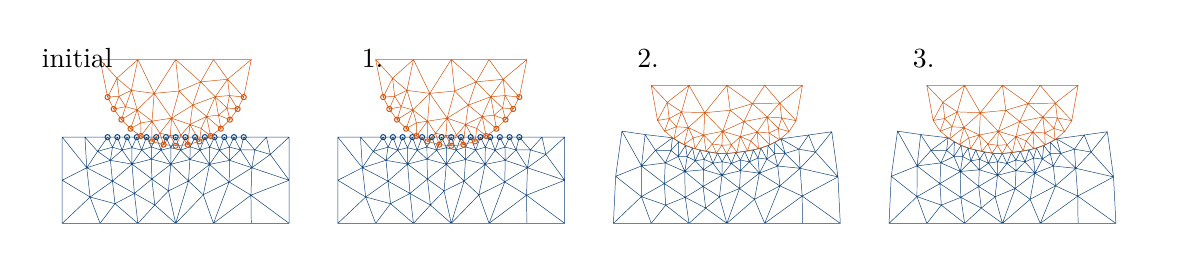
\begin{tikzpicture}
    
    \node at (-5.5, 0) {\scalebox{0.7}{%% Creator: Matplotlib, PGF backend
%%
%% To include the figure in your LaTeX document, write
%%   \input{<filename>.pgf}
%%
%% Make sure the required packages are loaded in your preamble
%%   \usepackage{pgf}
%%
%% Also ensure that all the required font packages are loaded; for instance,
%% the lmodern package is sometimes necessary when using math font.
%%   \usepackage{lmodern}
%%
%% Figures using additional raster images can only be included by \input if
%% they are in the same directory as the main LaTeX file. For loading figures
%% from other directories you can use the `import` package
%%   \usepackage{import}
%%
%% and then include the figures with
%%   \import{<path to file>}{<filename>.pgf}
%%
%% Matplotlib used the following preamble
%%   
%%   \usepackage{fontspec}
%%   \setmainfont{DejaVuSans.ttf}[Path=\detokenize{/home/fabio/Internodes-CM/.venv/lib/python3.8/site-packages/matplotlib/mpl-data/fonts/ttf/}]
%%   \setsansfont{DejaVuSans.ttf}[Path=\detokenize{/home/fabio/Internodes-CM/.venv/lib/python3.8/site-packages/matplotlib/mpl-data/fonts/ttf/}]
%%   \setmonofont{DejaVuSansMono.ttf}[Path=\detokenize{/home/fabio/Internodes-CM/.venv/lib/python3.8/site-packages/matplotlib/mpl-data/fonts/ttf/}]
%%   \makeatletter\@ifpackageloaded{underscore}{}{\usepackage[strings]{underscore}}\makeatother
%%
\begingroup%
\makeatletter%
\begin{pgfpicture}%
\pgfpathrectangle{\pgfpointorigin}{\pgfqpoint{1.982500in}{1.432000in}}%
\pgfusepath{use as bounding box, clip}%
\begin{pgfscope}%
\pgfsetbuttcap%
\pgfsetmiterjoin%
\definecolor{currentfill}{rgb}{1.000000,1.000000,1.000000}%
\pgfsetfillcolor{currentfill}%
\pgfsetlinewidth{0.000000pt}%
\definecolor{currentstroke}{rgb}{1.000000,1.000000,1.000000}%
\pgfsetstrokecolor{currentstroke}%
\pgfsetdash{}{0pt}%
\pgfpathmoveto{\pgfqpoint{0.000000in}{0.000000in}}%
\pgfpathlineto{\pgfqpoint{1.982500in}{0.000000in}}%
\pgfpathlineto{\pgfqpoint{1.982500in}{1.432000in}}%
\pgfpathlineto{\pgfqpoint{0.000000in}{1.432000in}}%
\pgfpathlineto{\pgfqpoint{0.000000in}{0.000000in}}%
\pgfpathclose%
\pgfusepath{fill}%
\end{pgfscope}%
\begin{pgfscope}%
\pgfpathrectangle{\pgfqpoint{0.100000in}{0.100000in}}{\pgfqpoint{1.782500in}{1.232000in}}%
\pgfusepath{clip}%
\pgfsetrectcap%
\pgfsetroundjoin%
\pgfsetlinewidth{0.250937pt}%
\definecolor{currentstroke}{rgb}{0.054902,0.262745,0.486275}%
\pgfsetstrokecolor{currentstroke}%
\pgfsetdash{}{0pt}%
\pgfpathmoveto{\pgfqpoint{0.451098in}{0.100000in}}%
\pgfpathlineto{\pgfqpoint{0.181023in}{0.100000in}}%
\pgfpathmoveto{\pgfqpoint{0.721174in}{0.100000in}}%
\pgfpathlineto{\pgfqpoint{0.451098in}{0.100000in}}%
\pgfpathmoveto{\pgfqpoint{0.991250in}{0.100000in}}%
\pgfpathlineto{\pgfqpoint{0.721174in}{0.100000in}}%
\pgfpathmoveto{\pgfqpoint{1.261326in}{0.100000in}}%
\pgfpathlineto{\pgfqpoint{0.991250in}{0.100000in}}%
\pgfpathmoveto{\pgfqpoint{1.531402in}{0.100000in}}%
\pgfpathlineto{\pgfqpoint{1.801477in}{0.100000in}}%
\pgfpathmoveto{\pgfqpoint{1.531402in}{0.100000in}}%
\pgfpathlineto{\pgfqpoint{1.261326in}{0.100000in}}%
\pgfpathmoveto{\pgfqpoint{1.801477in}{0.408000in}}%
\pgfpathlineto{\pgfqpoint{1.801477in}{0.100000in}}%
\pgfpathmoveto{\pgfqpoint{1.801477in}{0.408000in}}%
\pgfpathlineto{\pgfqpoint{1.801477in}{0.716000in}}%
\pgfpathmoveto{\pgfqpoint{1.639432in}{0.716000in}}%
\pgfpathlineto{\pgfqpoint{1.801477in}{0.716000in}}%
\pgfpathmoveto{\pgfqpoint{1.639432in}{0.716000in}}%
\pgfpathlineto{\pgfqpoint{1.477386in}{0.716000in}}%
\pgfpathmoveto{\pgfqpoint{1.407938in}{0.716000in}}%
\pgfpathlineto{\pgfqpoint{1.477386in}{0.716000in}}%
\pgfpathmoveto{\pgfqpoint{1.338490in}{0.716000in}}%
\pgfpathlineto{\pgfqpoint{1.407938in}{0.716000in}}%
\pgfpathmoveto{\pgfqpoint{1.269042in}{0.716000in}}%
\pgfpathlineto{\pgfqpoint{1.338490in}{0.716000in}}%
\pgfpathmoveto{\pgfqpoint{1.199594in}{0.716000in}}%
\pgfpathlineto{\pgfqpoint{1.269042in}{0.716000in}}%
\pgfpathmoveto{\pgfqpoint{1.130146in}{0.716000in}}%
\pgfpathlineto{\pgfqpoint{1.199594in}{0.716000in}}%
\pgfpathmoveto{\pgfqpoint{1.060698in}{0.716000in}}%
\pgfpathlineto{\pgfqpoint{1.130146in}{0.716000in}}%
\pgfpathmoveto{\pgfqpoint{0.991250in}{0.716000in}}%
\pgfpathlineto{\pgfqpoint{1.060698in}{0.716000in}}%
\pgfpathmoveto{\pgfqpoint{0.921802in}{0.716000in}}%
\pgfpathlineto{\pgfqpoint{0.991250in}{0.716000in}}%
\pgfpathmoveto{\pgfqpoint{0.852354in}{0.716000in}}%
\pgfpathlineto{\pgfqpoint{0.921802in}{0.716000in}}%
\pgfpathmoveto{\pgfqpoint{0.782906in}{0.716000in}}%
\pgfpathlineto{\pgfqpoint{0.852354in}{0.716000in}}%
\pgfpathmoveto{\pgfqpoint{0.713458in}{0.716000in}}%
\pgfpathlineto{\pgfqpoint{0.782906in}{0.716000in}}%
\pgfpathmoveto{\pgfqpoint{0.644010in}{0.716000in}}%
\pgfpathlineto{\pgfqpoint{0.713458in}{0.716000in}}%
\pgfpathmoveto{\pgfqpoint{0.574562in}{0.716000in}}%
\pgfpathlineto{\pgfqpoint{0.505114in}{0.716000in}}%
\pgfpathmoveto{\pgfqpoint{0.574562in}{0.716000in}}%
\pgfpathlineto{\pgfqpoint{0.644010in}{0.716000in}}%
\pgfpathmoveto{\pgfqpoint{0.343068in}{0.716000in}}%
\pgfpathlineto{\pgfqpoint{0.505114in}{0.716000in}}%
\pgfpathmoveto{\pgfqpoint{0.343068in}{0.716000in}}%
\pgfpathlineto{\pgfqpoint{0.181023in}{0.716000in}}%
\pgfpathmoveto{\pgfqpoint{0.181023in}{0.408000in}}%
\pgfpathlineto{\pgfqpoint{0.181023in}{0.100000in}}%
\pgfpathmoveto{\pgfqpoint{0.181023in}{0.408000in}}%
\pgfpathlineto{\pgfqpoint{0.181023in}{0.716000in}}%
\pgfpathmoveto{\pgfqpoint{1.373214in}{0.396057in}}%
\pgfpathlineto{\pgfqpoint{1.261326in}{0.100000in}}%
\pgfpathmoveto{\pgfqpoint{1.082944in}{0.402689in}}%
\pgfpathlineto{\pgfqpoint{0.991250in}{0.100000in}}%
\pgfpathmoveto{\pgfqpoint{1.233147in}{0.520967in}}%
\pgfpathlineto{\pgfqpoint{1.373214in}{0.396057in}}%
\pgfpathmoveto{\pgfqpoint{1.233147in}{0.520967in}}%
\pgfpathlineto{\pgfqpoint{1.082944in}{0.402689in}}%
\pgfpathmoveto{\pgfqpoint{0.956117in}{0.522274in}}%
\pgfpathlineto{\pgfqpoint{1.082944in}{0.402689in}}%
\pgfpathmoveto{\pgfqpoint{0.956117in}{0.522274in}}%
\pgfpathlineto{\pgfqpoint{0.821141in}{0.416705in}}%
\pgfpathmoveto{\pgfqpoint{0.679173in}{0.523635in}}%
\pgfpathlineto{\pgfqpoint{0.821141in}{0.416705in}}%
\pgfpathmoveto{\pgfqpoint{0.679173in}{0.523635in}}%
\pgfpathlineto{\pgfqpoint{0.539838in}{0.401685in}}%
\pgfpathmoveto{\pgfqpoint{1.535558in}{0.497212in}}%
\pgfpathlineto{\pgfqpoint{1.801477in}{0.408000in}}%
\pgfpathmoveto{\pgfqpoint{1.535558in}{0.497212in}}%
\pgfpathlineto{\pgfqpoint{1.373214in}{0.396057in}}%
\pgfpathmoveto{\pgfqpoint{1.376927in}{0.550483in}}%
\pgfpathlineto{\pgfqpoint{1.373214in}{0.396057in}}%
\pgfpathmoveto{\pgfqpoint{1.376927in}{0.550483in}}%
\pgfpathlineto{\pgfqpoint{1.233147in}{0.520967in}}%
\pgfpathmoveto{\pgfqpoint{1.376927in}{0.550483in}}%
\pgfpathlineto{\pgfqpoint{1.535558in}{0.497212in}}%
\pgfpathmoveto{\pgfqpoint{1.093079in}{0.556190in}}%
\pgfpathlineto{\pgfqpoint{1.082944in}{0.402689in}}%
\pgfpathmoveto{\pgfqpoint{1.093079in}{0.556190in}}%
\pgfpathlineto{\pgfqpoint{1.233147in}{0.520967in}}%
\pgfpathmoveto{\pgfqpoint{1.093079in}{0.556190in}}%
\pgfpathlineto{\pgfqpoint{0.956117in}{0.522274in}}%
\pgfpathmoveto{\pgfqpoint{0.818220in}{0.558974in}}%
\pgfpathlineto{\pgfqpoint{0.821141in}{0.416705in}}%
\pgfpathmoveto{\pgfqpoint{0.818220in}{0.558974in}}%
\pgfpathlineto{\pgfqpoint{0.956117in}{0.522274in}}%
\pgfpathmoveto{\pgfqpoint{0.818220in}{0.558974in}}%
\pgfpathlineto{\pgfqpoint{0.679173in}{0.523635in}}%
\pgfpathmoveto{\pgfqpoint{0.525112in}{0.550213in}}%
\pgfpathlineto{\pgfqpoint{0.539838in}{0.401685in}}%
\pgfpathmoveto{\pgfqpoint{0.525112in}{0.550213in}}%
\pgfpathlineto{\pgfqpoint{0.679173in}{0.523635in}}%
\pgfpathmoveto{\pgfqpoint{0.356186in}{0.497584in}}%
\pgfpathlineto{\pgfqpoint{0.181023in}{0.716000in}}%
\pgfpathmoveto{\pgfqpoint{0.356186in}{0.497584in}}%
\pgfpathlineto{\pgfqpoint{0.343068in}{0.716000in}}%
\pgfpathmoveto{\pgfqpoint{0.356186in}{0.497584in}}%
\pgfpathlineto{\pgfqpoint{0.181023in}{0.408000in}}%
\pgfpathmoveto{\pgfqpoint{0.356186in}{0.497584in}}%
\pgfpathlineto{\pgfqpoint{0.539838in}{0.401685in}}%
\pgfpathmoveto{\pgfqpoint{0.356186in}{0.497584in}}%
\pgfpathlineto{\pgfqpoint{0.525112in}{0.550213in}}%
\pgfpathmoveto{\pgfqpoint{1.303766in}{0.622307in}}%
\pgfpathlineto{\pgfqpoint{1.338490in}{0.716000in}}%
\pgfpathmoveto{\pgfqpoint{1.303766in}{0.622307in}}%
\pgfpathlineto{\pgfqpoint{1.269042in}{0.716000in}}%
\pgfpathmoveto{\pgfqpoint{1.303766in}{0.622307in}}%
\pgfpathlineto{\pgfqpoint{1.233147in}{0.520967in}}%
\pgfpathmoveto{\pgfqpoint{1.303766in}{0.622307in}}%
\pgfpathlineto{\pgfqpoint{1.376927in}{0.550483in}}%
\pgfpathmoveto{\pgfqpoint{1.164870in}{0.623450in}}%
\pgfpathlineto{\pgfqpoint{1.199594in}{0.716000in}}%
\pgfpathmoveto{\pgfqpoint{1.164870in}{0.623450in}}%
\pgfpathlineto{\pgfqpoint{1.130146in}{0.716000in}}%
\pgfpathmoveto{\pgfqpoint{1.164870in}{0.623450in}}%
\pgfpathlineto{\pgfqpoint{1.233147in}{0.520967in}}%
\pgfpathmoveto{\pgfqpoint{1.164870in}{0.623450in}}%
\pgfpathlineto{\pgfqpoint{1.093079in}{0.556190in}}%
\pgfpathmoveto{\pgfqpoint{1.025974in}{0.623450in}}%
\pgfpathlineto{\pgfqpoint{1.060698in}{0.716000in}}%
\pgfpathmoveto{\pgfqpoint{1.025974in}{0.623450in}}%
\pgfpathlineto{\pgfqpoint{0.991250in}{0.716000in}}%
\pgfpathmoveto{\pgfqpoint{1.025974in}{0.623450in}}%
\pgfpathlineto{\pgfqpoint{0.956117in}{0.522274in}}%
\pgfpathmoveto{\pgfqpoint{1.025974in}{0.623450in}}%
\pgfpathlineto{\pgfqpoint{1.093079in}{0.556190in}}%
\pgfpathmoveto{\pgfqpoint{0.887078in}{0.623460in}}%
\pgfpathlineto{\pgfqpoint{0.921802in}{0.716000in}}%
\pgfpathmoveto{\pgfqpoint{0.887078in}{0.623460in}}%
\pgfpathlineto{\pgfqpoint{0.852354in}{0.716000in}}%
\pgfpathmoveto{\pgfqpoint{0.887078in}{0.623460in}}%
\pgfpathlineto{\pgfqpoint{0.956117in}{0.522274in}}%
\pgfpathmoveto{\pgfqpoint{0.887078in}{0.623460in}}%
\pgfpathlineto{\pgfqpoint{0.818220in}{0.558974in}}%
\pgfpathmoveto{\pgfqpoint{0.748182in}{0.623460in}}%
\pgfpathlineto{\pgfqpoint{0.782906in}{0.716000in}}%
\pgfpathmoveto{\pgfqpoint{0.748182in}{0.623460in}}%
\pgfpathlineto{\pgfqpoint{0.713458in}{0.716000in}}%
\pgfpathmoveto{\pgfqpoint{0.748182in}{0.623460in}}%
\pgfpathlineto{\pgfqpoint{0.679173in}{0.523635in}}%
\pgfpathmoveto{\pgfqpoint{0.748182in}{0.623460in}}%
\pgfpathlineto{\pgfqpoint{0.818220in}{0.558974in}}%
\pgfpathmoveto{\pgfqpoint{0.609286in}{0.623460in}}%
\pgfpathlineto{\pgfqpoint{0.644010in}{0.716000in}}%
\pgfpathmoveto{\pgfqpoint{0.609286in}{0.623460in}}%
\pgfpathlineto{\pgfqpoint{0.574562in}{0.716000in}}%
\pgfpathmoveto{\pgfqpoint{0.609286in}{0.623460in}}%
\pgfpathlineto{\pgfqpoint{0.679173in}{0.523635in}}%
\pgfpathmoveto{\pgfqpoint{0.609286in}{0.623460in}}%
\pgfpathlineto{\pgfqpoint{0.525112in}{0.550213in}}%
\pgfpathmoveto{\pgfqpoint{1.453902in}{0.624729in}}%
\pgfpathlineto{\pgfqpoint{1.477386in}{0.716000in}}%
\pgfpathmoveto{\pgfqpoint{1.453902in}{0.624729in}}%
\pgfpathlineto{\pgfqpoint{1.407938in}{0.716000in}}%
\pgfpathmoveto{\pgfqpoint{1.453902in}{0.624729in}}%
\pgfpathlineto{\pgfqpoint{1.535558in}{0.497212in}}%
\pgfpathmoveto{\pgfqpoint{1.453902in}{0.624729in}}%
\pgfpathlineto{\pgfqpoint{1.376927in}{0.550483in}}%
\pgfpathmoveto{\pgfqpoint{0.939717in}{0.332038in}}%
\pgfpathlineto{\pgfqpoint{0.991250in}{0.100000in}}%
\pgfpathmoveto{\pgfqpoint{0.939717in}{0.332038in}}%
\pgfpathlineto{\pgfqpoint{1.082944in}{0.402689in}}%
\pgfpathmoveto{\pgfqpoint{0.939717in}{0.332038in}}%
\pgfpathlineto{\pgfqpoint{0.821141in}{0.416705in}}%
\pgfpathmoveto{\pgfqpoint{0.939717in}{0.332038in}}%
\pgfpathlineto{\pgfqpoint{0.956117in}{0.522274in}}%
\pgfpathmoveto{\pgfqpoint{0.433515in}{0.614303in}}%
\pgfpathlineto{\pgfqpoint{0.505114in}{0.716000in}}%
\pgfpathmoveto{\pgfqpoint{0.433515in}{0.614303in}}%
\pgfpathlineto{\pgfqpoint{0.343068in}{0.716000in}}%
\pgfpathmoveto{\pgfqpoint{0.433515in}{0.614303in}}%
\pgfpathlineto{\pgfqpoint{0.525112in}{0.550213in}}%
\pgfpathmoveto{\pgfqpoint{0.433515in}{0.614303in}}%
\pgfpathlineto{\pgfqpoint{0.356186in}{0.497584in}}%
\pgfpathmoveto{\pgfqpoint{1.374740in}{0.644995in}}%
\pgfpathlineto{\pgfqpoint{1.407938in}{0.716000in}}%
\pgfpathmoveto{\pgfqpoint{1.374740in}{0.644995in}}%
\pgfpathlineto{\pgfqpoint{1.338490in}{0.716000in}}%
\pgfpathmoveto{\pgfqpoint{1.374740in}{0.644995in}}%
\pgfpathlineto{\pgfqpoint{1.376927in}{0.550483in}}%
\pgfpathmoveto{\pgfqpoint{1.374740in}{0.644995in}}%
\pgfpathlineto{\pgfqpoint{1.303766in}{0.622307in}}%
\pgfpathmoveto{\pgfqpoint{1.374740in}{0.644995in}}%
\pgfpathlineto{\pgfqpoint{1.453902in}{0.624729in}}%
\pgfpathmoveto{\pgfqpoint{1.094954in}{0.647018in}}%
\pgfpathlineto{\pgfqpoint{1.130146in}{0.716000in}}%
\pgfpathmoveto{\pgfqpoint{1.094954in}{0.647018in}}%
\pgfpathlineto{\pgfqpoint{1.060698in}{0.716000in}}%
\pgfpathmoveto{\pgfqpoint{1.094954in}{0.647018in}}%
\pgfpathlineto{\pgfqpoint{1.093079in}{0.556190in}}%
\pgfpathmoveto{\pgfqpoint{1.094954in}{0.647018in}}%
\pgfpathlineto{\pgfqpoint{1.164870in}{0.623450in}}%
\pgfpathmoveto{\pgfqpoint{1.094954in}{0.647018in}}%
\pgfpathlineto{\pgfqpoint{1.025974in}{0.623450in}}%
\pgfpathmoveto{\pgfqpoint{1.234318in}{0.644309in}}%
\pgfpathlineto{\pgfqpoint{1.269042in}{0.716000in}}%
\pgfpathmoveto{\pgfqpoint{1.234318in}{0.644309in}}%
\pgfpathlineto{\pgfqpoint{1.199594in}{0.716000in}}%
\pgfpathmoveto{\pgfqpoint{1.234318in}{0.644309in}}%
\pgfpathlineto{\pgfqpoint{1.233147in}{0.520967in}}%
\pgfpathmoveto{\pgfqpoint{1.234318in}{0.644309in}}%
\pgfpathlineto{\pgfqpoint{1.303766in}{0.622307in}}%
\pgfpathmoveto{\pgfqpoint{1.234318in}{0.644309in}}%
\pgfpathlineto{\pgfqpoint{1.164870in}{0.623450in}}%
\pgfpathmoveto{\pgfqpoint{0.956444in}{0.640237in}}%
\pgfpathlineto{\pgfqpoint{0.991250in}{0.716000in}}%
\pgfpathmoveto{\pgfqpoint{0.956444in}{0.640237in}}%
\pgfpathlineto{\pgfqpoint{0.921802in}{0.716000in}}%
\pgfpathmoveto{\pgfqpoint{0.956444in}{0.640237in}}%
\pgfpathlineto{\pgfqpoint{0.956117in}{0.522274in}}%
\pgfpathmoveto{\pgfqpoint{0.956444in}{0.640237in}}%
\pgfpathlineto{\pgfqpoint{1.025974in}{0.623450in}}%
\pgfpathmoveto{\pgfqpoint{0.956444in}{0.640237in}}%
\pgfpathlineto{\pgfqpoint{0.887078in}{0.623460in}}%
\pgfpathmoveto{\pgfqpoint{0.817690in}{0.645978in}}%
\pgfpathlineto{\pgfqpoint{0.852354in}{0.716000in}}%
\pgfpathmoveto{\pgfqpoint{0.817690in}{0.645978in}}%
\pgfpathlineto{\pgfqpoint{0.782906in}{0.716000in}}%
\pgfpathmoveto{\pgfqpoint{0.817690in}{0.645978in}}%
\pgfpathlineto{\pgfqpoint{0.818220in}{0.558974in}}%
\pgfpathmoveto{\pgfqpoint{0.817690in}{0.645978in}}%
\pgfpathlineto{\pgfqpoint{0.887078in}{0.623460in}}%
\pgfpathmoveto{\pgfqpoint{0.817690in}{0.645978in}}%
\pgfpathlineto{\pgfqpoint{0.748182in}{0.623460in}}%
\pgfpathmoveto{\pgfqpoint{1.188376in}{0.303943in}}%
\pgfpathlineto{\pgfqpoint{0.991250in}{0.100000in}}%
\pgfpathmoveto{\pgfqpoint{1.188376in}{0.303943in}}%
\pgfpathlineto{\pgfqpoint{1.261326in}{0.100000in}}%
\pgfpathmoveto{\pgfqpoint{1.188376in}{0.303943in}}%
\pgfpathlineto{\pgfqpoint{1.373214in}{0.396057in}}%
\pgfpathmoveto{\pgfqpoint{1.188376in}{0.303943in}}%
\pgfpathlineto{\pgfqpoint{1.082944in}{0.402689in}}%
\pgfpathmoveto{\pgfqpoint{1.188376in}{0.303943in}}%
\pgfpathlineto{\pgfqpoint{1.233147in}{0.520967in}}%
\pgfpathmoveto{\pgfqpoint{0.696453in}{0.313796in}}%
\pgfpathlineto{\pgfqpoint{0.721174in}{0.100000in}}%
\pgfpathmoveto{\pgfqpoint{0.696453in}{0.313796in}}%
\pgfpathlineto{\pgfqpoint{0.821141in}{0.416705in}}%
\pgfpathmoveto{\pgfqpoint{0.696453in}{0.313796in}}%
\pgfpathlineto{\pgfqpoint{0.539838in}{0.401685in}}%
\pgfpathmoveto{\pgfqpoint{0.696453in}{0.313796in}}%
\pgfpathlineto{\pgfqpoint{0.679173in}{0.523635in}}%
\pgfpathmoveto{\pgfqpoint{0.678822in}{0.640511in}}%
\pgfpathlineto{\pgfqpoint{0.713458in}{0.716000in}}%
\pgfpathmoveto{\pgfqpoint{0.678822in}{0.640511in}}%
\pgfpathlineto{\pgfqpoint{0.644010in}{0.716000in}}%
\pgfpathmoveto{\pgfqpoint{0.678822in}{0.640511in}}%
\pgfpathlineto{\pgfqpoint{0.679173in}{0.523635in}}%
\pgfpathmoveto{\pgfqpoint{0.678822in}{0.640511in}}%
\pgfpathlineto{\pgfqpoint{0.748182in}{0.623460in}}%
\pgfpathmoveto{\pgfqpoint{0.678822in}{0.640511in}}%
\pgfpathlineto{\pgfqpoint{0.609286in}{0.623460in}}%
\pgfpathmoveto{\pgfqpoint{1.556669in}{0.624742in}}%
\pgfpathlineto{\pgfqpoint{1.477386in}{0.716000in}}%
\pgfpathmoveto{\pgfqpoint{1.556669in}{0.624742in}}%
\pgfpathlineto{\pgfqpoint{1.639432in}{0.716000in}}%
\pgfpathmoveto{\pgfqpoint{1.556669in}{0.624742in}}%
\pgfpathlineto{\pgfqpoint{1.535558in}{0.497212in}}%
\pgfpathmoveto{\pgfqpoint{1.556669in}{0.624742in}}%
\pgfpathlineto{\pgfqpoint{1.453902in}{0.624729in}}%
\pgfpathmoveto{\pgfqpoint{0.539838in}{0.644311in}}%
\pgfpathlineto{\pgfqpoint{0.505114in}{0.716000in}}%
\pgfpathmoveto{\pgfqpoint{0.539838in}{0.644311in}}%
\pgfpathlineto{\pgfqpoint{0.574562in}{0.716000in}}%
\pgfpathmoveto{\pgfqpoint{0.539838in}{0.644311in}}%
\pgfpathlineto{\pgfqpoint{0.525112in}{0.550213in}}%
\pgfpathmoveto{\pgfqpoint{0.539838in}{0.644311in}}%
\pgfpathlineto{\pgfqpoint{0.609286in}{0.623460in}}%
\pgfpathmoveto{\pgfqpoint{0.539838in}{0.644311in}}%
\pgfpathlineto{\pgfqpoint{0.433515in}{0.614303in}}%
\pgfpathmoveto{\pgfqpoint{0.379905in}{0.288250in}}%
\pgfpathlineto{\pgfqpoint{0.181023in}{0.100000in}}%
\pgfpathmoveto{\pgfqpoint{0.379905in}{0.288250in}}%
\pgfpathlineto{\pgfqpoint{0.451098in}{0.100000in}}%
\pgfpathmoveto{\pgfqpoint{0.379905in}{0.288250in}}%
\pgfpathlineto{\pgfqpoint{0.181023in}{0.408000in}}%
\pgfpathmoveto{\pgfqpoint{0.379905in}{0.288250in}}%
\pgfpathlineto{\pgfqpoint{0.539838in}{0.401685in}}%
\pgfpathmoveto{\pgfqpoint{0.379905in}{0.288250in}}%
\pgfpathlineto{\pgfqpoint{0.356186in}{0.497584in}}%
\pgfpathmoveto{\pgfqpoint{1.528881in}{0.301240in}}%
\pgfpathlineto{\pgfqpoint{1.801477in}{0.100000in}}%
\pgfpathmoveto{\pgfqpoint{1.528881in}{0.301240in}}%
\pgfpathlineto{\pgfqpoint{1.261326in}{0.100000in}}%
\pgfpathmoveto{\pgfqpoint{1.528881in}{0.301240in}}%
\pgfpathlineto{\pgfqpoint{1.531402in}{0.100000in}}%
\pgfpathmoveto{\pgfqpoint{1.528881in}{0.301240in}}%
\pgfpathlineto{\pgfqpoint{1.801477in}{0.408000in}}%
\pgfpathmoveto{\pgfqpoint{1.528881in}{0.301240in}}%
\pgfpathlineto{\pgfqpoint{1.373214in}{0.396057in}}%
\pgfpathmoveto{\pgfqpoint{1.528881in}{0.301240in}}%
\pgfpathlineto{\pgfqpoint{1.535558in}{0.497212in}}%
\pgfpathmoveto{\pgfqpoint{1.666923in}{0.592391in}}%
\pgfpathlineto{\pgfqpoint{1.801477in}{0.716000in}}%
\pgfpathmoveto{\pgfqpoint{1.666923in}{0.592391in}}%
\pgfpathlineto{\pgfqpoint{1.801477in}{0.408000in}}%
\pgfpathmoveto{\pgfqpoint{1.666923in}{0.592391in}}%
\pgfpathlineto{\pgfqpoint{1.639432in}{0.716000in}}%
\pgfpathmoveto{\pgfqpoint{1.666923in}{0.592391in}}%
\pgfpathlineto{\pgfqpoint{1.535558in}{0.497212in}}%
\pgfpathmoveto{\pgfqpoint{1.666923in}{0.592391in}}%
\pgfpathlineto{\pgfqpoint{1.556669in}{0.624742in}}%
\pgfpathmoveto{\pgfqpoint{0.842327in}{0.230907in}}%
\pgfpathlineto{\pgfqpoint{0.721174in}{0.100000in}}%
\pgfpathmoveto{\pgfqpoint{0.842327in}{0.230907in}}%
\pgfpathlineto{\pgfqpoint{0.991250in}{0.100000in}}%
\pgfpathmoveto{\pgfqpoint{0.842327in}{0.230907in}}%
\pgfpathlineto{\pgfqpoint{0.821141in}{0.416705in}}%
\pgfpathmoveto{\pgfqpoint{0.842327in}{0.230907in}}%
\pgfpathlineto{\pgfqpoint{0.939717in}{0.332038in}}%
\pgfpathmoveto{\pgfqpoint{0.842327in}{0.230907in}}%
\pgfpathlineto{\pgfqpoint{0.696453in}{0.313796in}}%
\pgfpathmoveto{\pgfqpoint{0.557694in}{0.240746in}}%
\pgfpathlineto{\pgfqpoint{0.451098in}{0.100000in}}%
\pgfpathmoveto{\pgfqpoint{0.557694in}{0.240746in}}%
\pgfpathlineto{\pgfqpoint{0.721174in}{0.100000in}}%
\pgfpathmoveto{\pgfqpoint{0.557694in}{0.240746in}}%
\pgfpathlineto{\pgfqpoint{0.539838in}{0.401685in}}%
\pgfpathmoveto{\pgfqpoint{0.557694in}{0.240746in}}%
\pgfpathlineto{\pgfqpoint{0.696453in}{0.313796in}}%
\pgfpathmoveto{\pgfqpoint{0.557694in}{0.240746in}}%
\pgfpathlineto{\pgfqpoint{0.379905in}{0.288250in}}%
\pgfpathlineto{\pgfqpoint{0.379905in}{0.288250in}}%
\pgfusepath{stroke}%
\end{pgfscope}%
\begin{pgfscope}%
\pgfpathrectangle{\pgfqpoint{0.100000in}{0.100000in}}{\pgfqpoint{1.782500in}{1.232000in}}%
\pgfusepath{clip}%
\pgfsetrectcap%
\pgfsetroundjoin%
\pgfsetlinewidth{0.250937pt}%
\definecolor{currentstroke}{rgb}{0.835294,0.321569,0.035294}%
\pgfsetstrokecolor{currentstroke}%
\pgfsetdash{}{0pt}%
\pgfpathmoveto{\pgfqpoint{0.505114in}{1.001892in}}%
\pgfpathlineto{\pgfqpoint{0.451098in}{1.270400in}}%
\pgfpathmoveto{\pgfqpoint{1.531402in}{1.270400in}}%
\pgfpathlineto{\pgfqpoint{1.477386in}{1.001892in}}%
\pgfpathmoveto{\pgfqpoint{0.721174in}{1.270400in}}%
\pgfpathlineto{\pgfqpoint{0.991250in}{1.270400in}}%
\pgfpathmoveto{\pgfqpoint{0.721174in}{1.270400in}}%
\pgfpathlineto{\pgfqpoint{0.451098in}{1.270400in}}%
\pgfpathmoveto{\pgfqpoint{0.548824in}{0.917012in}}%
\pgfpathlineto{\pgfqpoint{0.505114in}{1.001892in}}%
\pgfpathmoveto{\pgfqpoint{0.603831in}{0.841156in}}%
\pgfpathlineto{\pgfqpoint{0.548824in}{0.917012in}}%
\pgfpathmoveto{\pgfqpoint{0.668731in}{0.776261in}}%
\pgfpathlineto{\pgfqpoint{0.603831in}{0.841156in}}%
\pgfpathmoveto{\pgfqpoint{0.741867in}{0.723983in}}%
\pgfpathlineto{\pgfqpoint{0.668731in}{0.776261in}}%
\pgfpathmoveto{\pgfqpoint{0.821370in}{0.685658in}}%
\pgfpathlineto{\pgfqpoint{0.741867in}{0.723983in}}%
\pgfpathmoveto{\pgfqpoint{0.905212in}{0.662265in}}%
\pgfpathlineto{\pgfqpoint{0.821370in}{0.685658in}}%
\pgfpathmoveto{\pgfqpoint{0.991250in}{0.654400in}}%
\pgfpathlineto{\pgfqpoint{0.905212in}{0.662265in}}%
\pgfpathmoveto{\pgfqpoint{1.077288in}{0.662265in}}%
\pgfpathlineto{\pgfqpoint{0.991250in}{0.654400in}}%
\pgfpathmoveto{\pgfqpoint{1.161130in}{0.685658in}}%
\pgfpathlineto{\pgfqpoint{1.077288in}{0.662265in}}%
\pgfpathmoveto{\pgfqpoint{1.240633in}{0.723983in}}%
\pgfpathlineto{\pgfqpoint{1.161130in}{0.685658in}}%
\pgfpathmoveto{\pgfqpoint{1.313769in}{0.776261in}}%
\pgfpathlineto{\pgfqpoint{1.240633in}{0.723983in}}%
\pgfpathmoveto{\pgfqpoint{1.378669in}{0.841156in}}%
\pgfpathlineto{\pgfqpoint{1.313769in}{0.776261in}}%
\pgfpathmoveto{\pgfqpoint{1.433676in}{0.917012in}}%
\pgfpathlineto{\pgfqpoint{1.477386in}{1.001892in}}%
\pgfpathmoveto{\pgfqpoint{1.433676in}{0.917012in}}%
\pgfpathlineto{\pgfqpoint{1.378669in}{0.841156in}}%
\pgfpathmoveto{\pgfqpoint{1.261326in}{1.270400in}}%
\pgfpathlineto{\pgfqpoint{0.991250in}{1.270400in}}%
\pgfpathmoveto{\pgfqpoint{1.261326in}{1.270400in}}%
\pgfpathlineto{\pgfqpoint{1.531402in}{1.270400in}}%
\pgfpathmoveto{\pgfqpoint{0.837830in}{1.028470in}}%
\pgfpathlineto{\pgfqpoint{0.991250in}{1.270400in}}%
\pgfpathmoveto{\pgfqpoint{0.837830in}{1.028470in}}%
\pgfpathlineto{\pgfqpoint{0.721174in}{1.270400in}}%
\pgfpathmoveto{\pgfqpoint{0.961801in}{0.851412in}}%
\pgfpathlineto{\pgfqpoint{1.113091in}{0.944697in}}%
\pgfpathmoveto{\pgfqpoint{0.961801in}{0.851412in}}%
\pgfpathlineto{\pgfqpoint{0.837830in}{1.028470in}}%
\pgfpathmoveto{\pgfqpoint{1.273497in}{1.004211in}}%
\pgfpathlineto{\pgfqpoint{1.113091in}{0.944697in}}%
\pgfpathmoveto{\pgfqpoint{0.674832in}{1.049989in}}%
\pgfpathlineto{\pgfqpoint{0.721174in}{1.270400in}}%
\pgfpathmoveto{\pgfqpoint{0.674832in}{1.049989in}}%
\pgfpathlineto{\pgfqpoint{0.837830in}{1.028470in}}%
\pgfpathmoveto{\pgfqpoint{1.093189in}{0.806475in}}%
\pgfpathlineto{\pgfqpoint{1.077288in}{0.662265in}}%
\pgfpathmoveto{\pgfqpoint{1.093189in}{0.806475in}}%
\pgfpathlineto{\pgfqpoint{1.161130in}{0.685658in}}%
\pgfpathmoveto{\pgfqpoint{1.093189in}{0.806475in}}%
\pgfpathlineto{\pgfqpoint{1.113091in}{0.944697in}}%
\pgfpathmoveto{\pgfqpoint{1.093189in}{0.806475in}}%
\pgfpathlineto{\pgfqpoint{0.961801in}{0.851412in}}%
\pgfpathmoveto{\pgfqpoint{1.212025in}{0.863682in}}%
\pgfpathlineto{\pgfqpoint{1.240633in}{0.723983in}}%
\pgfpathmoveto{\pgfqpoint{1.212025in}{0.863682in}}%
\pgfpathlineto{\pgfqpoint{1.313769in}{0.776261in}}%
\pgfpathmoveto{\pgfqpoint{1.212025in}{0.863682in}}%
\pgfpathlineto{\pgfqpoint{1.113091in}{0.944697in}}%
\pgfpathmoveto{\pgfqpoint{1.212025in}{0.863682in}}%
\pgfpathlineto{\pgfqpoint{1.273497in}{1.004211in}}%
\pgfpathmoveto{\pgfqpoint{1.212025in}{0.863682in}}%
\pgfpathlineto{\pgfqpoint{1.093189in}{0.806475in}}%
\pgfpathmoveto{\pgfqpoint{0.822435in}{0.830135in}}%
\pgfpathlineto{\pgfqpoint{0.741867in}{0.723983in}}%
\pgfpathmoveto{\pgfqpoint{0.822435in}{0.830135in}}%
\pgfpathlineto{\pgfqpoint{0.821370in}{0.685658in}}%
\pgfpathmoveto{\pgfqpoint{0.822435in}{0.830135in}}%
\pgfpathlineto{\pgfqpoint{0.837830in}{1.028470in}}%
\pgfpathmoveto{\pgfqpoint{0.822435in}{0.830135in}}%
\pgfpathlineto{\pgfqpoint{0.961801in}{0.851412in}}%
\pgfpathmoveto{\pgfqpoint{0.716798in}{0.910757in}}%
\pgfpathlineto{\pgfqpoint{0.603831in}{0.841156in}}%
\pgfpathmoveto{\pgfqpoint{0.716798in}{0.910757in}}%
\pgfpathlineto{\pgfqpoint{0.668731in}{0.776261in}}%
\pgfpathmoveto{\pgfqpoint{0.716798in}{0.910757in}}%
\pgfpathlineto{\pgfqpoint{0.837830in}{1.028470in}}%
\pgfpathmoveto{\pgfqpoint{0.716798in}{0.910757in}}%
\pgfpathlineto{\pgfqpoint{0.674832in}{1.049989in}}%
\pgfpathmoveto{\pgfqpoint{0.716798in}{0.910757in}}%
\pgfpathlineto{\pgfqpoint{0.822435in}{0.830135in}}%
\pgfpathmoveto{\pgfqpoint{1.362495in}{1.129252in}}%
\pgfpathlineto{\pgfqpoint{1.477386in}{1.001892in}}%
\pgfpathmoveto{\pgfqpoint{1.362495in}{1.129252in}}%
\pgfpathlineto{\pgfqpoint{1.531402in}{1.270400in}}%
\pgfpathmoveto{\pgfqpoint{1.362495in}{1.129252in}}%
\pgfpathlineto{\pgfqpoint{1.261326in}{1.270400in}}%
\pgfpathmoveto{\pgfqpoint{1.362495in}{1.129252in}}%
\pgfpathlineto{\pgfqpoint{1.273497in}{1.004211in}}%
\pgfpathmoveto{\pgfqpoint{0.953154in}{0.728383in}}%
\pgfpathlineto{\pgfqpoint{0.905212in}{0.662265in}}%
\pgfpathmoveto{\pgfqpoint{0.953154in}{0.728383in}}%
\pgfpathlineto{\pgfqpoint{0.991250in}{0.654400in}}%
\pgfpathmoveto{\pgfqpoint{0.953154in}{0.728383in}}%
\pgfpathlineto{\pgfqpoint{0.961801in}{0.851412in}}%
\pgfpathmoveto{\pgfqpoint{1.297122in}{0.872566in}}%
\pgfpathlineto{\pgfqpoint{1.313769in}{0.776261in}}%
\pgfpathmoveto{\pgfqpoint{1.297122in}{0.872566in}}%
\pgfpathlineto{\pgfqpoint{1.378669in}{0.841156in}}%
\pgfpathmoveto{\pgfqpoint{1.297122in}{0.872566in}}%
\pgfpathlineto{\pgfqpoint{1.273497in}{1.004211in}}%
\pgfpathmoveto{\pgfqpoint{1.297122in}{0.872566in}}%
\pgfpathlineto{\pgfqpoint{1.212025in}{0.863682in}}%
\pgfpathmoveto{\pgfqpoint{1.173657in}{0.778274in}}%
\pgfpathlineto{\pgfqpoint{1.161130in}{0.685658in}}%
\pgfpathmoveto{\pgfqpoint{1.173657in}{0.778274in}}%
\pgfpathlineto{\pgfqpoint{1.240633in}{0.723983in}}%
\pgfpathmoveto{\pgfqpoint{1.173657in}{0.778274in}}%
\pgfpathlineto{\pgfqpoint{1.093189in}{0.806475in}}%
\pgfpathmoveto{\pgfqpoint{1.173657in}{0.778274in}}%
\pgfpathlineto{\pgfqpoint{1.212025in}{0.863682in}}%
\pgfpathmoveto{\pgfqpoint{1.375529in}{1.013033in}}%
\pgfpathlineto{\pgfqpoint{1.477386in}{1.001892in}}%
\pgfpathmoveto{\pgfqpoint{1.375529in}{1.013033in}}%
\pgfpathlineto{\pgfqpoint{1.433676in}{0.917012in}}%
\pgfpathmoveto{\pgfqpoint{1.375529in}{1.013033in}}%
\pgfpathlineto{\pgfqpoint{1.273497in}{1.004211in}}%
\pgfpathmoveto{\pgfqpoint{1.375529in}{1.013033in}}%
\pgfpathlineto{\pgfqpoint{1.362495in}{1.129252in}}%
\pgfpathmoveto{\pgfqpoint{0.742156in}{0.817783in}}%
\pgfpathlineto{\pgfqpoint{0.668731in}{0.776261in}}%
\pgfpathmoveto{\pgfqpoint{0.742156in}{0.817783in}}%
\pgfpathlineto{\pgfqpoint{0.741867in}{0.723983in}}%
\pgfpathmoveto{\pgfqpoint{0.742156in}{0.817783in}}%
\pgfpathlineto{\pgfqpoint{0.822435in}{0.830135in}}%
\pgfpathmoveto{\pgfqpoint{0.742156in}{0.817783in}}%
\pgfpathlineto{\pgfqpoint{0.716798in}{0.910757in}}%
\pgfpathmoveto{\pgfqpoint{0.633716in}{0.933208in}}%
\pgfpathlineto{\pgfqpoint{0.548824in}{0.917012in}}%
\pgfpathmoveto{\pgfqpoint{0.633716in}{0.933208in}}%
\pgfpathlineto{\pgfqpoint{0.603831in}{0.841156in}}%
\pgfpathmoveto{\pgfqpoint{0.633716in}{0.933208in}}%
\pgfpathlineto{\pgfqpoint{0.674832in}{1.049989in}}%
\pgfpathmoveto{\pgfqpoint{0.633716in}{0.933208in}}%
\pgfpathlineto{\pgfqpoint{0.716798in}{0.910757in}}%
\pgfpathmoveto{\pgfqpoint{0.572102in}{1.136818in}}%
\pgfpathlineto{\pgfqpoint{0.451098in}{1.270400in}}%
\pgfpathmoveto{\pgfqpoint{0.572102in}{1.136818in}}%
\pgfpathlineto{\pgfqpoint{0.505114in}{1.001892in}}%
\pgfpathmoveto{\pgfqpoint{0.572102in}{1.136818in}}%
\pgfpathlineto{\pgfqpoint{0.721174in}{1.270400in}}%
\pgfpathmoveto{\pgfqpoint{0.572102in}{1.136818in}}%
\pgfpathlineto{\pgfqpoint{0.674832in}{1.049989in}}%
\pgfpathmoveto{\pgfqpoint{1.029231in}{0.730021in}}%
\pgfpathlineto{\pgfqpoint{0.991250in}{0.654400in}}%
\pgfpathmoveto{\pgfqpoint{1.029231in}{0.730021in}}%
\pgfpathlineto{\pgfqpoint{1.077288in}{0.662265in}}%
\pgfpathmoveto{\pgfqpoint{1.029231in}{0.730021in}}%
\pgfpathlineto{\pgfqpoint{0.961801in}{0.851412in}}%
\pgfpathmoveto{\pgfqpoint{1.029231in}{0.730021in}}%
\pgfpathlineto{\pgfqpoint{1.093189in}{0.806475in}}%
\pgfpathmoveto{\pgfqpoint{1.029231in}{0.730021in}}%
\pgfpathlineto{\pgfqpoint{0.953154in}{0.728383in}}%
\pgfpathmoveto{\pgfqpoint{0.878278in}{0.743820in}}%
\pgfpathlineto{\pgfqpoint{0.821370in}{0.685658in}}%
\pgfpathmoveto{\pgfqpoint{0.878278in}{0.743820in}}%
\pgfpathlineto{\pgfqpoint{0.905212in}{0.662265in}}%
\pgfpathmoveto{\pgfqpoint{0.878278in}{0.743820in}}%
\pgfpathlineto{\pgfqpoint{0.961801in}{0.851412in}}%
\pgfpathmoveto{\pgfqpoint{0.878278in}{0.743820in}}%
\pgfpathlineto{\pgfqpoint{0.822435in}{0.830135in}}%
\pgfpathmoveto{\pgfqpoint{0.878278in}{0.743820in}}%
\pgfpathlineto{\pgfqpoint{0.953154in}{0.728383in}}%
\pgfpathmoveto{\pgfqpoint{1.357947in}{0.924566in}}%
\pgfpathlineto{\pgfqpoint{1.378669in}{0.841156in}}%
\pgfpathmoveto{\pgfqpoint{1.357947in}{0.924566in}}%
\pgfpathlineto{\pgfqpoint{1.433676in}{0.917012in}}%
\pgfpathmoveto{\pgfqpoint{1.357947in}{0.924566in}}%
\pgfpathlineto{\pgfqpoint{1.273497in}{1.004211in}}%
\pgfpathmoveto{\pgfqpoint{1.357947in}{0.924566in}}%
\pgfpathlineto{\pgfqpoint{1.297122in}{0.872566in}}%
\pgfpathmoveto{\pgfqpoint{1.357947in}{0.924566in}}%
\pgfpathlineto{\pgfqpoint{1.375529in}{1.013033in}}%
\pgfpathmoveto{\pgfqpoint{1.015627in}{1.045348in}}%
\pgfpathlineto{\pgfqpoint{0.991250in}{1.270400in}}%
\pgfpathmoveto{\pgfqpoint{1.015627in}{1.045348in}}%
\pgfpathlineto{\pgfqpoint{1.113091in}{0.944697in}}%
\pgfpathmoveto{\pgfqpoint{1.015627in}{1.045348in}}%
\pgfpathlineto{\pgfqpoint{0.837830in}{1.028470in}}%
\pgfpathmoveto{\pgfqpoint{1.015627in}{1.045348in}}%
\pgfpathlineto{\pgfqpoint{0.961801in}{0.851412in}}%
\pgfpathmoveto{\pgfqpoint{1.169547in}{1.110718in}}%
\pgfpathlineto{\pgfqpoint{0.991250in}{1.270400in}}%
\pgfpathmoveto{\pgfqpoint{1.169547in}{1.110718in}}%
\pgfpathlineto{\pgfqpoint{1.261326in}{1.270400in}}%
\pgfpathmoveto{\pgfqpoint{1.169547in}{1.110718in}}%
\pgfpathlineto{\pgfqpoint{1.113091in}{0.944697in}}%
\pgfpathmoveto{\pgfqpoint{1.169547in}{1.110718in}}%
\pgfpathlineto{\pgfqpoint{1.273497in}{1.004211in}}%
\pgfpathmoveto{\pgfqpoint{1.169547in}{1.110718in}}%
\pgfpathlineto{\pgfqpoint{1.362495in}{1.129252in}}%
\pgfpathmoveto{\pgfqpoint{1.169547in}{1.110718in}}%
\pgfpathlineto{\pgfqpoint{1.015627in}{1.045348in}}%
\pgfpathmoveto{\pgfqpoint{0.586918in}{1.007784in}}%
\pgfpathlineto{\pgfqpoint{0.505114in}{1.001892in}}%
\pgfpathmoveto{\pgfqpoint{0.586918in}{1.007784in}}%
\pgfpathlineto{\pgfqpoint{0.548824in}{0.917012in}}%
\pgfpathmoveto{\pgfqpoint{0.586918in}{1.007784in}}%
\pgfpathlineto{\pgfqpoint{0.674832in}{1.049989in}}%
\pgfpathmoveto{\pgfqpoint{0.586918in}{1.007784in}}%
\pgfpathlineto{\pgfqpoint{0.633716in}{0.933208in}}%
\pgfpathmoveto{\pgfqpoint{0.586918in}{1.007784in}}%
\pgfpathlineto{\pgfqpoint{0.572102in}{1.136818in}}%
\pgfpathlineto{\pgfqpoint{0.572102in}{1.136818in}}%
\pgfusepath{stroke}%
\end{pgfscope}%
\begin{pgfscope}%
\pgfpathrectangle{\pgfqpoint{0.100000in}{0.100000in}}{\pgfqpoint{1.782500in}{1.232000in}}%
\pgfusepath{clip}%
\pgfsetbuttcap%
\pgfsetroundjoin%
\pgfsetlinewidth{0.501875pt}%
\definecolor{currentstroke}{rgb}{0.054902,0.262745,0.486275}%
\pgfsetstrokecolor{currentstroke}%
\pgfsetdash{}{0pt}%
\pgfpathmoveto{\pgfqpoint{1.477386in}{0.697627in}}%
\pgfpathcurveto{\pgfqpoint{1.482259in}{0.697627in}}{\pgfqpoint{1.486933in}{0.699563in}}{\pgfqpoint{1.490378in}{0.703008in}}%
\pgfpathcurveto{\pgfqpoint{1.493824in}{0.706454in}}{\pgfqpoint{1.495760in}{0.711127in}}{\pgfqpoint{1.495760in}{0.716000in}}%
\pgfpathcurveto{\pgfqpoint{1.495760in}{0.720873in}}{\pgfqpoint{1.493824in}{0.725546in}}{\pgfqpoint{1.490378in}{0.728992in}}%
\pgfpathcurveto{\pgfqpoint{1.486933in}{0.732437in}}{\pgfqpoint{1.482259in}{0.734373in}}{\pgfqpoint{1.477386in}{0.734373in}}%
\pgfpathcurveto{\pgfqpoint{1.472514in}{0.734373in}}{\pgfqpoint{1.467840in}{0.732437in}}{\pgfqpoint{1.464394in}{0.728992in}}%
\pgfpathcurveto{\pgfqpoint{1.460949in}{0.725546in}}{\pgfqpoint{1.459013in}{0.720873in}}{\pgfqpoint{1.459013in}{0.716000in}}%
\pgfpathcurveto{\pgfqpoint{1.459013in}{0.711127in}}{\pgfqpoint{1.460949in}{0.706454in}}{\pgfqpoint{1.464394in}{0.703008in}}%
\pgfpathcurveto{\pgfqpoint{1.467840in}{0.699563in}}{\pgfqpoint{1.472514in}{0.697627in}}{\pgfqpoint{1.477386in}{0.697627in}}%
\pgfpathlineto{\pgfqpoint{1.477386in}{0.697627in}}%
\pgfpathclose%
\pgfusepath{stroke}%
\end{pgfscope}%
\begin{pgfscope}%
\pgfpathrectangle{\pgfqpoint{0.100000in}{0.100000in}}{\pgfqpoint{1.782500in}{1.232000in}}%
\pgfusepath{clip}%
\pgfsetbuttcap%
\pgfsetroundjoin%
\pgfsetlinewidth{0.501875pt}%
\definecolor{currentstroke}{rgb}{0.054902,0.262745,0.486275}%
\pgfsetstrokecolor{currentstroke}%
\pgfsetdash{}{0pt}%
\pgfpathmoveto{\pgfqpoint{0.505114in}{0.697627in}}%
\pgfpathcurveto{\pgfqpoint{0.509986in}{0.697627in}}{\pgfqpoint{0.514660in}{0.699563in}}{\pgfqpoint{0.518106in}{0.703008in}}%
\pgfpathcurveto{\pgfqpoint{0.521551in}{0.706454in}}{\pgfqpoint{0.523487in}{0.711127in}}{\pgfqpoint{0.523487in}{0.716000in}}%
\pgfpathcurveto{\pgfqpoint{0.523487in}{0.720873in}}{\pgfqpoint{0.521551in}{0.725546in}}{\pgfqpoint{0.518106in}{0.728992in}}%
\pgfpathcurveto{\pgfqpoint{0.514660in}{0.732437in}}{\pgfqpoint{0.509986in}{0.734373in}}{\pgfqpoint{0.505114in}{0.734373in}}%
\pgfpathcurveto{\pgfqpoint{0.500241in}{0.734373in}}{\pgfqpoint{0.495567in}{0.732437in}}{\pgfqpoint{0.492122in}{0.728992in}}%
\pgfpathcurveto{\pgfqpoint{0.488676in}{0.725546in}}{\pgfqpoint{0.486740in}{0.720873in}}{\pgfqpoint{0.486740in}{0.716000in}}%
\pgfpathcurveto{\pgfqpoint{0.486740in}{0.711127in}}{\pgfqpoint{0.488676in}{0.706454in}}{\pgfqpoint{0.492122in}{0.703008in}}%
\pgfpathcurveto{\pgfqpoint{0.495567in}{0.699563in}}{\pgfqpoint{0.500241in}{0.697627in}}{\pgfqpoint{0.505114in}{0.697627in}}%
\pgfpathlineto{\pgfqpoint{0.505114in}{0.697627in}}%
\pgfpathclose%
\pgfusepath{stroke}%
\end{pgfscope}%
\begin{pgfscope}%
\pgfpathrectangle{\pgfqpoint{0.100000in}{0.100000in}}{\pgfqpoint{1.782500in}{1.232000in}}%
\pgfusepath{clip}%
\pgfsetbuttcap%
\pgfsetroundjoin%
\pgfsetlinewidth{0.501875pt}%
\definecolor{currentstroke}{rgb}{0.054902,0.262745,0.486275}%
\pgfsetstrokecolor{currentstroke}%
\pgfsetdash{}{0pt}%
\pgfpathmoveto{\pgfqpoint{1.407938in}{0.697627in}}%
\pgfpathcurveto{\pgfqpoint{1.412811in}{0.697627in}}{\pgfqpoint{1.417485in}{0.699563in}}{\pgfqpoint{1.420930in}{0.703008in}}%
\pgfpathcurveto{\pgfqpoint{1.424376in}{0.706454in}}{\pgfqpoint{1.426312in}{0.711127in}}{\pgfqpoint{1.426312in}{0.716000in}}%
\pgfpathcurveto{\pgfqpoint{1.426312in}{0.720873in}}{\pgfqpoint{1.424376in}{0.725546in}}{\pgfqpoint{1.420930in}{0.728992in}}%
\pgfpathcurveto{\pgfqpoint{1.417485in}{0.732437in}}{\pgfqpoint{1.412811in}{0.734373in}}{\pgfqpoint{1.407938in}{0.734373in}}%
\pgfpathcurveto{\pgfqpoint{1.403066in}{0.734373in}}{\pgfqpoint{1.398392in}{0.732437in}}{\pgfqpoint{1.394946in}{0.728992in}}%
\pgfpathcurveto{\pgfqpoint{1.391501in}{0.725546in}}{\pgfqpoint{1.389565in}{0.720873in}}{\pgfqpoint{1.389565in}{0.716000in}}%
\pgfpathcurveto{\pgfqpoint{1.389565in}{0.711127in}}{\pgfqpoint{1.391501in}{0.706454in}}{\pgfqpoint{1.394946in}{0.703008in}}%
\pgfpathcurveto{\pgfqpoint{1.398392in}{0.699563in}}{\pgfqpoint{1.403066in}{0.697627in}}{\pgfqpoint{1.407938in}{0.697627in}}%
\pgfpathlineto{\pgfqpoint{1.407938in}{0.697627in}}%
\pgfpathclose%
\pgfusepath{stroke}%
\end{pgfscope}%
\begin{pgfscope}%
\pgfpathrectangle{\pgfqpoint{0.100000in}{0.100000in}}{\pgfqpoint{1.782500in}{1.232000in}}%
\pgfusepath{clip}%
\pgfsetbuttcap%
\pgfsetroundjoin%
\pgfsetlinewidth{0.501875pt}%
\definecolor{currentstroke}{rgb}{0.054902,0.262745,0.486275}%
\pgfsetstrokecolor{currentstroke}%
\pgfsetdash{}{0pt}%
\pgfpathmoveto{\pgfqpoint{1.338490in}{0.697627in}}%
\pgfpathcurveto{\pgfqpoint{1.343363in}{0.697627in}}{\pgfqpoint{1.348037in}{0.699563in}}{\pgfqpoint{1.351482in}{0.703008in}}%
\pgfpathcurveto{\pgfqpoint{1.354928in}{0.706454in}}{\pgfqpoint{1.356864in}{0.711127in}}{\pgfqpoint{1.356864in}{0.716000in}}%
\pgfpathcurveto{\pgfqpoint{1.356864in}{0.720873in}}{\pgfqpoint{1.354928in}{0.725546in}}{\pgfqpoint{1.351482in}{0.728992in}}%
\pgfpathcurveto{\pgfqpoint{1.348037in}{0.732437in}}{\pgfqpoint{1.343363in}{0.734373in}}{\pgfqpoint{1.338490in}{0.734373in}}%
\pgfpathcurveto{\pgfqpoint{1.333618in}{0.734373in}}{\pgfqpoint{1.328944in}{0.732437in}}{\pgfqpoint{1.325498in}{0.728992in}}%
\pgfpathcurveto{\pgfqpoint{1.322053in}{0.725546in}}{\pgfqpoint{1.320117in}{0.720873in}}{\pgfqpoint{1.320117in}{0.716000in}}%
\pgfpathcurveto{\pgfqpoint{1.320117in}{0.711127in}}{\pgfqpoint{1.322053in}{0.706454in}}{\pgfqpoint{1.325498in}{0.703008in}}%
\pgfpathcurveto{\pgfqpoint{1.328944in}{0.699563in}}{\pgfqpoint{1.333618in}{0.697627in}}{\pgfqpoint{1.338490in}{0.697627in}}%
\pgfpathlineto{\pgfqpoint{1.338490in}{0.697627in}}%
\pgfpathclose%
\pgfusepath{stroke}%
\end{pgfscope}%
\begin{pgfscope}%
\pgfpathrectangle{\pgfqpoint{0.100000in}{0.100000in}}{\pgfqpoint{1.782500in}{1.232000in}}%
\pgfusepath{clip}%
\pgfsetbuttcap%
\pgfsetroundjoin%
\pgfsetlinewidth{0.501875pt}%
\definecolor{currentstroke}{rgb}{0.054902,0.262745,0.486275}%
\pgfsetstrokecolor{currentstroke}%
\pgfsetdash{}{0pt}%
\pgfpathmoveto{\pgfqpoint{1.269042in}{0.697627in}}%
\pgfpathcurveto{\pgfqpoint{1.273915in}{0.697627in}}{\pgfqpoint{1.278589in}{0.699563in}}{\pgfqpoint{1.282034in}{0.703008in}}%
\pgfpathcurveto{\pgfqpoint{1.285480in}{0.706454in}}{\pgfqpoint{1.287415in}{0.711127in}}{\pgfqpoint{1.287415in}{0.716000in}}%
\pgfpathcurveto{\pgfqpoint{1.287415in}{0.720873in}}{\pgfqpoint{1.285480in}{0.725546in}}{\pgfqpoint{1.282034in}{0.728992in}}%
\pgfpathcurveto{\pgfqpoint{1.278589in}{0.732437in}}{\pgfqpoint{1.273915in}{0.734373in}}{\pgfqpoint{1.269042in}{0.734373in}}%
\pgfpathcurveto{\pgfqpoint{1.264170in}{0.734373in}}{\pgfqpoint{1.259496in}{0.732437in}}{\pgfqpoint{1.256050in}{0.728992in}}%
\pgfpathcurveto{\pgfqpoint{1.252605in}{0.725546in}}{\pgfqpoint{1.250669in}{0.720873in}}{\pgfqpoint{1.250669in}{0.716000in}}%
\pgfpathcurveto{\pgfqpoint{1.250669in}{0.711127in}}{\pgfqpoint{1.252605in}{0.706454in}}{\pgfqpoint{1.256050in}{0.703008in}}%
\pgfpathcurveto{\pgfqpoint{1.259496in}{0.699563in}}{\pgfqpoint{1.264170in}{0.697627in}}{\pgfqpoint{1.269042in}{0.697627in}}%
\pgfpathlineto{\pgfqpoint{1.269042in}{0.697627in}}%
\pgfpathclose%
\pgfusepath{stroke}%
\end{pgfscope}%
\begin{pgfscope}%
\pgfpathrectangle{\pgfqpoint{0.100000in}{0.100000in}}{\pgfqpoint{1.782500in}{1.232000in}}%
\pgfusepath{clip}%
\pgfsetbuttcap%
\pgfsetroundjoin%
\pgfsetlinewidth{0.501875pt}%
\definecolor{currentstroke}{rgb}{0.054902,0.262745,0.486275}%
\pgfsetstrokecolor{currentstroke}%
\pgfsetdash{}{0pt}%
\pgfpathmoveto{\pgfqpoint{1.199594in}{0.697627in}}%
\pgfpathcurveto{\pgfqpoint{1.204467in}{0.697627in}}{\pgfqpoint{1.209141in}{0.699563in}}{\pgfqpoint{1.212586in}{0.703008in}}%
\pgfpathcurveto{\pgfqpoint{1.216032in}{0.706454in}}{\pgfqpoint{1.217967in}{0.711127in}}{\pgfqpoint{1.217967in}{0.716000in}}%
\pgfpathcurveto{\pgfqpoint{1.217967in}{0.720873in}}{\pgfqpoint{1.216032in}{0.725546in}}{\pgfqpoint{1.212586in}{0.728992in}}%
\pgfpathcurveto{\pgfqpoint{1.209141in}{0.732437in}}{\pgfqpoint{1.204467in}{0.734373in}}{\pgfqpoint{1.199594in}{0.734373in}}%
\pgfpathcurveto{\pgfqpoint{1.194722in}{0.734373in}}{\pgfqpoint{1.190048in}{0.732437in}}{\pgfqpoint{1.186602in}{0.728992in}}%
\pgfpathcurveto{\pgfqpoint{1.183157in}{0.725546in}}{\pgfqpoint{1.181221in}{0.720873in}}{\pgfqpoint{1.181221in}{0.716000in}}%
\pgfpathcurveto{\pgfqpoint{1.181221in}{0.711127in}}{\pgfqpoint{1.183157in}{0.706454in}}{\pgfqpoint{1.186602in}{0.703008in}}%
\pgfpathcurveto{\pgfqpoint{1.190048in}{0.699563in}}{\pgfqpoint{1.194722in}{0.697627in}}{\pgfqpoint{1.199594in}{0.697627in}}%
\pgfpathlineto{\pgfqpoint{1.199594in}{0.697627in}}%
\pgfpathclose%
\pgfusepath{stroke}%
\end{pgfscope}%
\begin{pgfscope}%
\pgfpathrectangle{\pgfqpoint{0.100000in}{0.100000in}}{\pgfqpoint{1.782500in}{1.232000in}}%
\pgfusepath{clip}%
\pgfsetbuttcap%
\pgfsetroundjoin%
\pgfsetlinewidth{0.501875pt}%
\definecolor{currentstroke}{rgb}{0.054902,0.262745,0.486275}%
\pgfsetstrokecolor{currentstroke}%
\pgfsetdash{}{0pt}%
\pgfpathmoveto{\pgfqpoint{1.130146in}{0.697627in}}%
\pgfpathcurveto{\pgfqpoint{1.135019in}{0.697627in}}{\pgfqpoint{1.139692in}{0.699563in}}{\pgfqpoint{1.143138in}{0.703008in}}%
\pgfpathcurveto{\pgfqpoint{1.146583in}{0.706454in}}{\pgfqpoint{1.148519in}{0.711127in}}{\pgfqpoint{1.148519in}{0.716000in}}%
\pgfpathcurveto{\pgfqpoint{1.148519in}{0.720873in}}{\pgfqpoint{1.146583in}{0.725546in}}{\pgfqpoint{1.143138in}{0.728992in}}%
\pgfpathcurveto{\pgfqpoint{1.139692in}{0.732437in}}{\pgfqpoint{1.135019in}{0.734373in}}{\pgfqpoint{1.130146in}{0.734373in}}%
\pgfpathcurveto{\pgfqpoint{1.125273in}{0.734373in}}{\pgfqpoint{1.120600in}{0.732437in}}{\pgfqpoint{1.117154in}{0.728992in}}%
\pgfpathcurveto{\pgfqpoint{1.113709in}{0.725546in}}{\pgfqpoint{1.111773in}{0.720873in}}{\pgfqpoint{1.111773in}{0.716000in}}%
\pgfpathcurveto{\pgfqpoint{1.111773in}{0.711127in}}{\pgfqpoint{1.113709in}{0.706454in}}{\pgfqpoint{1.117154in}{0.703008in}}%
\pgfpathcurveto{\pgfqpoint{1.120600in}{0.699563in}}{\pgfqpoint{1.125273in}{0.697627in}}{\pgfqpoint{1.130146in}{0.697627in}}%
\pgfpathlineto{\pgfqpoint{1.130146in}{0.697627in}}%
\pgfpathclose%
\pgfusepath{stroke}%
\end{pgfscope}%
\begin{pgfscope}%
\pgfpathrectangle{\pgfqpoint{0.100000in}{0.100000in}}{\pgfqpoint{1.782500in}{1.232000in}}%
\pgfusepath{clip}%
\pgfsetbuttcap%
\pgfsetroundjoin%
\pgfsetlinewidth{0.501875pt}%
\definecolor{currentstroke}{rgb}{0.054902,0.262745,0.486275}%
\pgfsetstrokecolor{currentstroke}%
\pgfsetdash{}{0pt}%
\pgfpathmoveto{\pgfqpoint{1.060698in}{0.697627in}}%
\pgfpathcurveto{\pgfqpoint{1.065571in}{0.697627in}}{\pgfqpoint{1.070244in}{0.699563in}}{\pgfqpoint{1.073690in}{0.703008in}}%
\pgfpathcurveto{\pgfqpoint{1.077135in}{0.706454in}}{\pgfqpoint{1.079071in}{0.711127in}}{\pgfqpoint{1.079071in}{0.716000in}}%
\pgfpathcurveto{\pgfqpoint{1.079071in}{0.720873in}}{\pgfqpoint{1.077135in}{0.725546in}}{\pgfqpoint{1.073690in}{0.728992in}}%
\pgfpathcurveto{\pgfqpoint{1.070244in}{0.732437in}}{\pgfqpoint{1.065571in}{0.734373in}}{\pgfqpoint{1.060698in}{0.734373in}}%
\pgfpathcurveto{\pgfqpoint{1.055825in}{0.734373in}}{\pgfqpoint{1.051152in}{0.732437in}}{\pgfqpoint{1.047706in}{0.728992in}}%
\pgfpathcurveto{\pgfqpoint{1.044261in}{0.725546in}}{\pgfqpoint{1.042325in}{0.720873in}}{\pgfqpoint{1.042325in}{0.716000in}}%
\pgfpathcurveto{\pgfqpoint{1.042325in}{0.711127in}}{\pgfqpoint{1.044261in}{0.706454in}}{\pgfqpoint{1.047706in}{0.703008in}}%
\pgfpathcurveto{\pgfqpoint{1.051152in}{0.699563in}}{\pgfqpoint{1.055825in}{0.697627in}}{\pgfqpoint{1.060698in}{0.697627in}}%
\pgfpathlineto{\pgfqpoint{1.060698in}{0.697627in}}%
\pgfpathclose%
\pgfusepath{stroke}%
\end{pgfscope}%
\begin{pgfscope}%
\pgfpathrectangle{\pgfqpoint{0.100000in}{0.100000in}}{\pgfqpoint{1.782500in}{1.232000in}}%
\pgfusepath{clip}%
\pgfsetbuttcap%
\pgfsetroundjoin%
\pgfsetlinewidth{0.501875pt}%
\definecolor{currentstroke}{rgb}{0.054902,0.262745,0.486275}%
\pgfsetstrokecolor{currentstroke}%
\pgfsetdash{}{0pt}%
\pgfpathmoveto{\pgfqpoint{0.991250in}{0.697627in}}%
\pgfpathcurveto{\pgfqpoint{0.996123in}{0.697627in}}{\pgfqpoint{1.000796in}{0.699563in}}{\pgfqpoint{1.004242in}{0.703008in}}%
\pgfpathcurveto{\pgfqpoint{1.007687in}{0.706454in}}{\pgfqpoint{1.009623in}{0.711127in}}{\pgfqpoint{1.009623in}{0.716000in}}%
\pgfpathcurveto{\pgfqpoint{1.009623in}{0.720873in}}{\pgfqpoint{1.007687in}{0.725546in}}{\pgfqpoint{1.004242in}{0.728992in}}%
\pgfpathcurveto{\pgfqpoint{1.000796in}{0.732437in}}{\pgfqpoint{0.996123in}{0.734373in}}{\pgfqpoint{0.991250in}{0.734373in}}%
\pgfpathcurveto{\pgfqpoint{0.986377in}{0.734373in}}{\pgfqpoint{0.981704in}{0.732437in}}{\pgfqpoint{0.978258in}{0.728992in}}%
\pgfpathcurveto{\pgfqpoint{0.974813in}{0.725546in}}{\pgfqpoint{0.972877in}{0.720873in}}{\pgfqpoint{0.972877in}{0.716000in}}%
\pgfpathcurveto{\pgfqpoint{0.972877in}{0.711127in}}{\pgfqpoint{0.974813in}{0.706454in}}{\pgfqpoint{0.978258in}{0.703008in}}%
\pgfpathcurveto{\pgfqpoint{0.981704in}{0.699563in}}{\pgfqpoint{0.986377in}{0.697627in}}{\pgfqpoint{0.991250in}{0.697627in}}%
\pgfpathlineto{\pgfqpoint{0.991250in}{0.697627in}}%
\pgfpathclose%
\pgfusepath{stroke}%
\end{pgfscope}%
\begin{pgfscope}%
\pgfpathrectangle{\pgfqpoint{0.100000in}{0.100000in}}{\pgfqpoint{1.782500in}{1.232000in}}%
\pgfusepath{clip}%
\pgfsetbuttcap%
\pgfsetroundjoin%
\pgfsetlinewidth{0.501875pt}%
\definecolor{currentstroke}{rgb}{0.054902,0.262745,0.486275}%
\pgfsetstrokecolor{currentstroke}%
\pgfsetdash{}{0pt}%
\pgfpathmoveto{\pgfqpoint{0.921802in}{0.697627in}}%
\pgfpathcurveto{\pgfqpoint{0.926675in}{0.697627in}}{\pgfqpoint{0.931348in}{0.699563in}}{\pgfqpoint{0.934794in}{0.703008in}}%
\pgfpathcurveto{\pgfqpoint{0.938239in}{0.706454in}}{\pgfqpoint{0.940175in}{0.711127in}}{\pgfqpoint{0.940175in}{0.716000in}}%
\pgfpathcurveto{\pgfqpoint{0.940175in}{0.720873in}}{\pgfqpoint{0.938239in}{0.725546in}}{\pgfqpoint{0.934794in}{0.728992in}}%
\pgfpathcurveto{\pgfqpoint{0.931348in}{0.732437in}}{\pgfqpoint{0.926675in}{0.734373in}}{\pgfqpoint{0.921802in}{0.734373in}}%
\pgfpathcurveto{\pgfqpoint{0.916929in}{0.734373in}}{\pgfqpoint{0.912256in}{0.732437in}}{\pgfqpoint{0.908810in}{0.728992in}}%
\pgfpathcurveto{\pgfqpoint{0.905365in}{0.725546in}}{\pgfqpoint{0.903429in}{0.720873in}}{\pgfqpoint{0.903429in}{0.716000in}}%
\pgfpathcurveto{\pgfqpoint{0.903429in}{0.711127in}}{\pgfqpoint{0.905365in}{0.706454in}}{\pgfqpoint{0.908810in}{0.703008in}}%
\pgfpathcurveto{\pgfqpoint{0.912256in}{0.699563in}}{\pgfqpoint{0.916929in}{0.697627in}}{\pgfqpoint{0.921802in}{0.697627in}}%
\pgfpathlineto{\pgfqpoint{0.921802in}{0.697627in}}%
\pgfpathclose%
\pgfusepath{stroke}%
\end{pgfscope}%
\begin{pgfscope}%
\pgfpathrectangle{\pgfqpoint{0.100000in}{0.100000in}}{\pgfqpoint{1.782500in}{1.232000in}}%
\pgfusepath{clip}%
\pgfsetbuttcap%
\pgfsetroundjoin%
\pgfsetlinewidth{0.501875pt}%
\definecolor{currentstroke}{rgb}{0.054902,0.262745,0.486275}%
\pgfsetstrokecolor{currentstroke}%
\pgfsetdash{}{0pt}%
\pgfpathmoveto{\pgfqpoint{0.852354in}{0.697627in}}%
\pgfpathcurveto{\pgfqpoint{0.857227in}{0.697627in}}{\pgfqpoint{0.861900in}{0.699563in}}{\pgfqpoint{0.865346in}{0.703008in}}%
\pgfpathcurveto{\pgfqpoint{0.868791in}{0.706454in}}{\pgfqpoint{0.870727in}{0.711127in}}{\pgfqpoint{0.870727in}{0.716000in}}%
\pgfpathcurveto{\pgfqpoint{0.870727in}{0.720873in}}{\pgfqpoint{0.868791in}{0.725546in}}{\pgfqpoint{0.865346in}{0.728992in}}%
\pgfpathcurveto{\pgfqpoint{0.861900in}{0.732437in}}{\pgfqpoint{0.857227in}{0.734373in}}{\pgfqpoint{0.852354in}{0.734373in}}%
\pgfpathcurveto{\pgfqpoint{0.847481in}{0.734373in}}{\pgfqpoint{0.842808in}{0.732437in}}{\pgfqpoint{0.839362in}{0.728992in}}%
\pgfpathcurveto{\pgfqpoint{0.835917in}{0.725546in}}{\pgfqpoint{0.833981in}{0.720873in}}{\pgfqpoint{0.833981in}{0.716000in}}%
\pgfpathcurveto{\pgfqpoint{0.833981in}{0.711127in}}{\pgfqpoint{0.835917in}{0.706454in}}{\pgfqpoint{0.839362in}{0.703008in}}%
\pgfpathcurveto{\pgfqpoint{0.842808in}{0.699563in}}{\pgfqpoint{0.847481in}{0.697627in}}{\pgfqpoint{0.852354in}{0.697627in}}%
\pgfpathlineto{\pgfqpoint{0.852354in}{0.697627in}}%
\pgfpathclose%
\pgfusepath{stroke}%
\end{pgfscope}%
\begin{pgfscope}%
\pgfpathrectangle{\pgfqpoint{0.100000in}{0.100000in}}{\pgfqpoint{1.782500in}{1.232000in}}%
\pgfusepath{clip}%
\pgfsetbuttcap%
\pgfsetroundjoin%
\pgfsetlinewidth{0.501875pt}%
\definecolor{currentstroke}{rgb}{0.054902,0.262745,0.486275}%
\pgfsetstrokecolor{currentstroke}%
\pgfsetdash{}{0pt}%
\pgfpathmoveto{\pgfqpoint{0.782906in}{0.697627in}}%
\pgfpathcurveto{\pgfqpoint{0.787778in}{0.697627in}}{\pgfqpoint{0.792452in}{0.699563in}}{\pgfqpoint{0.795898in}{0.703008in}}%
\pgfpathcurveto{\pgfqpoint{0.799343in}{0.706454in}}{\pgfqpoint{0.801279in}{0.711127in}}{\pgfqpoint{0.801279in}{0.716000in}}%
\pgfpathcurveto{\pgfqpoint{0.801279in}{0.720873in}}{\pgfqpoint{0.799343in}{0.725546in}}{\pgfqpoint{0.795898in}{0.728992in}}%
\pgfpathcurveto{\pgfqpoint{0.792452in}{0.732437in}}{\pgfqpoint{0.787778in}{0.734373in}}{\pgfqpoint{0.782906in}{0.734373in}}%
\pgfpathcurveto{\pgfqpoint{0.778033in}{0.734373in}}{\pgfqpoint{0.773359in}{0.732437in}}{\pgfqpoint{0.769914in}{0.728992in}}%
\pgfpathcurveto{\pgfqpoint{0.766468in}{0.725546in}}{\pgfqpoint{0.764533in}{0.720873in}}{\pgfqpoint{0.764533in}{0.716000in}}%
\pgfpathcurveto{\pgfqpoint{0.764533in}{0.711127in}}{\pgfqpoint{0.766468in}{0.706454in}}{\pgfqpoint{0.769914in}{0.703008in}}%
\pgfpathcurveto{\pgfqpoint{0.773359in}{0.699563in}}{\pgfqpoint{0.778033in}{0.697627in}}{\pgfqpoint{0.782906in}{0.697627in}}%
\pgfpathlineto{\pgfqpoint{0.782906in}{0.697627in}}%
\pgfpathclose%
\pgfusepath{stroke}%
\end{pgfscope}%
\begin{pgfscope}%
\pgfpathrectangle{\pgfqpoint{0.100000in}{0.100000in}}{\pgfqpoint{1.782500in}{1.232000in}}%
\pgfusepath{clip}%
\pgfsetbuttcap%
\pgfsetroundjoin%
\pgfsetlinewidth{0.501875pt}%
\definecolor{currentstroke}{rgb}{0.054902,0.262745,0.486275}%
\pgfsetstrokecolor{currentstroke}%
\pgfsetdash{}{0pt}%
\pgfpathmoveto{\pgfqpoint{0.713458in}{0.697627in}}%
\pgfpathcurveto{\pgfqpoint{0.718330in}{0.697627in}}{\pgfqpoint{0.723004in}{0.699563in}}{\pgfqpoint{0.726450in}{0.703008in}}%
\pgfpathcurveto{\pgfqpoint{0.729895in}{0.706454in}}{\pgfqpoint{0.731831in}{0.711127in}}{\pgfqpoint{0.731831in}{0.716000in}}%
\pgfpathcurveto{\pgfqpoint{0.731831in}{0.720873in}}{\pgfqpoint{0.729895in}{0.725546in}}{\pgfqpoint{0.726450in}{0.728992in}}%
\pgfpathcurveto{\pgfqpoint{0.723004in}{0.732437in}}{\pgfqpoint{0.718330in}{0.734373in}}{\pgfqpoint{0.713458in}{0.734373in}}%
\pgfpathcurveto{\pgfqpoint{0.708585in}{0.734373in}}{\pgfqpoint{0.703911in}{0.732437in}}{\pgfqpoint{0.700466in}{0.728992in}}%
\pgfpathcurveto{\pgfqpoint{0.697020in}{0.725546in}}{\pgfqpoint{0.695085in}{0.720873in}}{\pgfqpoint{0.695085in}{0.716000in}}%
\pgfpathcurveto{\pgfqpoint{0.695085in}{0.711127in}}{\pgfqpoint{0.697020in}{0.706454in}}{\pgfqpoint{0.700466in}{0.703008in}}%
\pgfpathcurveto{\pgfqpoint{0.703911in}{0.699563in}}{\pgfqpoint{0.708585in}{0.697627in}}{\pgfqpoint{0.713458in}{0.697627in}}%
\pgfpathlineto{\pgfqpoint{0.713458in}{0.697627in}}%
\pgfpathclose%
\pgfusepath{stroke}%
\end{pgfscope}%
\begin{pgfscope}%
\pgfpathrectangle{\pgfqpoint{0.100000in}{0.100000in}}{\pgfqpoint{1.782500in}{1.232000in}}%
\pgfusepath{clip}%
\pgfsetbuttcap%
\pgfsetroundjoin%
\pgfsetlinewidth{0.501875pt}%
\definecolor{currentstroke}{rgb}{0.054902,0.262745,0.486275}%
\pgfsetstrokecolor{currentstroke}%
\pgfsetdash{}{0pt}%
\pgfpathmoveto{\pgfqpoint{0.644010in}{0.697627in}}%
\pgfpathcurveto{\pgfqpoint{0.648882in}{0.697627in}}{\pgfqpoint{0.653556in}{0.699563in}}{\pgfqpoint{0.657002in}{0.703008in}}%
\pgfpathcurveto{\pgfqpoint{0.660447in}{0.706454in}}{\pgfqpoint{0.662383in}{0.711127in}}{\pgfqpoint{0.662383in}{0.716000in}}%
\pgfpathcurveto{\pgfqpoint{0.662383in}{0.720873in}}{\pgfqpoint{0.660447in}{0.725546in}}{\pgfqpoint{0.657002in}{0.728992in}}%
\pgfpathcurveto{\pgfqpoint{0.653556in}{0.732437in}}{\pgfqpoint{0.648882in}{0.734373in}}{\pgfqpoint{0.644010in}{0.734373in}}%
\pgfpathcurveto{\pgfqpoint{0.639137in}{0.734373in}}{\pgfqpoint{0.634463in}{0.732437in}}{\pgfqpoint{0.631018in}{0.728992in}}%
\pgfpathcurveto{\pgfqpoint{0.627572in}{0.725546in}}{\pgfqpoint{0.625636in}{0.720873in}}{\pgfqpoint{0.625636in}{0.716000in}}%
\pgfpathcurveto{\pgfqpoint{0.625636in}{0.711127in}}{\pgfqpoint{0.627572in}{0.706454in}}{\pgfqpoint{0.631018in}{0.703008in}}%
\pgfpathcurveto{\pgfqpoint{0.634463in}{0.699563in}}{\pgfqpoint{0.639137in}{0.697627in}}{\pgfqpoint{0.644010in}{0.697627in}}%
\pgfpathlineto{\pgfqpoint{0.644010in}{0.697627in}}%
\pgfpathclose%
\pgfusepath{stroke}%
\end{pgfscope}%
\begin{pgfscope}%
\pgfpathrectangle{\pgfqpoint{0.100000in}{0.100000in}}{\pgfqpoint{1.782500in}{1.232000in}}%
\pgfusepath{clip}%
\pgfsetbuttcap%
\pgfsetroundjoin%
\pgfsetlinewidth{0.501875pt}%
\definecolor{currentstroke}{rgb}{0.054902,0.262745,0.486275}%
\pgfsetstrokecolor{currentstroke}%
\pgfsetdash{}{0pt}%
\pgfpathmoveto{\pgfqpoint{0.574562in}{0.697627in}}%
\pgfpathcurveto{\pgfqpoint{0.579434in}{0.697627in}}{\pgfqpoint{0.584108in}{0.699563in}}{\pgfqpoint{0.587554in}{0.703008in}}%
\pgfpathcurveto{\pgfqpoint{0.590999in}{0.706454in}}{\pgfqpoint{0.592935in}{0.711127in}}{\pgfqpoint{0.592935in}{0.716000in}}%
\pgfpathcurveto{\pgfqpoint{0.592935in}{0.720873in}}{\pgfqpoint{0.590999in}{0.725546in}}{\pgfqpoint{0.587554in}{0.728992in}}%
\pgfpathcurveto{\pgfqpoint{0.584108in}{0.732437in}}{\pgfqpoint{0.579434in}{0.734373in}}{\pgfqpoint{0.574562in}{0.734373in}}%
\pgfpathcurveto{\pgfqpoint{0.569689in}{0.734373in}}{\pgfqpoint{0.565015in}{0.732437in}}{\pgfqpoint{0.561570in}{0.728992in}}%
\pgfpathcurveto{\pgfqpoint{0.558124in}{0.725546in}}{\pgfqpoint{0.556188in}{0.720873in}}{\pgfqpoint{0.556188in}{0.716000in}}%
\pgfpathcurveto{\pgfqpoint{0.556188in}{0.711127in}}{\pgfqpoint{0.558124in}{0.706454in}}{\pgfqpoint{0.561570in}{0.703008in}}%
\pgfpathcurveto{\pgfqpoint{0.565015in}{0.699563in}}{\pgfqpoint{0.569689in}{0.697627in}}{\pgfqpoint{0.574562in}{0.697627in}}%
\pgfpathlineto{\pgfqpoint{0.574562in}{0.697627in}}%
\pgfpathclose%
\pgfusepath{stroke}%
\end{pgfscope}%
\begin{pgfscope}%
\pgfpathrectangle{\pgfqpoint{0.100000in}{0.100000in}}{\pgfqpoint{1.782500in}{1.232000in}}%
\pgfusepath{clip}%
\pgfsetbuttcap%
\pgfsetroundjoin%
\pgfsetlinewidth{0.501875pt}%
\definecolor{currentstroke}{rgb}{0.835294,0.321569,0.035294}%
\pgfsetstrokecolor{currentstroke}%
\pgfsetdash{}{0pt}%
\pgfpathmoveto{\pgfqpoint{0.505114in}{0.983519in}}%
\pgfpathcurveto{\pgfqpoint{0.509986in}{0.983519in}}{\pgfqpoint{0.514660in}{0.985454in}}{\pgfqpoint{0.518106in}{0.988900in}}%
\pgfpathcurveto{\pgfqpoint{0.521551in}{0.992345in}}{\pgfqpoint{0.523487in}{0.997019in}}{\pgfqpoint{0.523487in}{1.001892in}}%
\pgfpathcurveto{\pgfqpoint{0.523487in}{1.006764in}}{\pgfqpoint{0.521551in}{1.011438in}}{\pgfqpoint{0.518106in}{1.014884in}}%
\pgfpathcurveto{\pgfqpoint{0.514660in}{1.018329in}}{\pgfqpoint{0.509986in}{1.020265in}}{\pgfqpoint{0.505114in}{1.020265in}}%
\pgfpathcurveto{\pgfqpoint{0.500241in}{1.020265in}}{\pgfqpoint{0.495567in}{1.018329in}}{\pgfqpoint{0.492122in}{1.014884in}}%
\pgfpathcurveto{\pgfqpoint{0.488676in}{1.011438in}}{\pgfqpoint{0.486740in}{1.006764in}}{\pgfqpoint{0.486740in}{1.001892in}}%
\pgfpathcurveto{\pgfqpoint{0.486740in}{0.997019in}}{\pgfqpoint{0.488676in}{0.992345in}}{\pgfqpoint{0.492122in}{0.988900in}}%
\pgfpathcurveto{\pgfqpoint{0.495567in}{0.985454in}}{\pgfqpoint{0.500241in}{0.983519in}}{\pgfqpoint{0.505114in}{0.983519in}}%
\pgfpathlineto{\pgfqpoint{0.505114in}{0.983519in}}%
\pgfpathclose%
\pgfusepath{stroke}%
\end{pgfscope}%
\begin{pgfscope}%
\pgfpathrectangle{\pgfqpoint{0.100000in}{0.100000in}}{\pgfqpoint{1.782500in}{1.232000in}}%
\pgfusepath{clip}%
\pgfsetbuttcap%
\pgfsetroundjoin%
\pgfsetlinewidth{0.501875pt}%
\definecolor{currentstroke}{rgb}{0.835294,0.321569,0.035294}%
\pgfsetstrokecolor{currentstroke}%
\pgfsetdash{}{0pt}%
\pgfpathmoveto{\pgfqpoint{1.477386in}{0.983519in}}%
\pgfpathcurveto{\pgfqpoint{1.482259in}{0.983519in}}{\pgfqpoint{1.486933in}{0.985454in}}{\pgfqpoint{1.490378in}{0.988900in}}%
\pgfpathcurveto{\pgfqpoint{1.493824in}{0.992345in}}{\pgfqpoint{1.495760in}{0.997019in}}{\pgfqpoint{1.495760in}{1.001892in}}%
\pgfpathcurveto{\pgfqpoint{1.495760in}{1.006764in}}{\pgfqpoint{1.493824in}{1.011438in}}{\pgfqpoint{1.490378in}{1.014884in}}%
\pgfpathcurveto{\pgfqpoint{1.486933in}{1.018329in}}{\pgfqpoint{1.482259in}{1.020265in}}{\pgfqpoint{1.477386in}{1.020265in}}%
\pgfpathcurveto{\pgfqpoint{1.472514in}{1.020265in}}{\pgfqpoint{1.467840in}{1.018329in}}{\pgfqpoint{1.464394in}{1.014884in}}%
\pgfpathcurveto{\pgfqpoint{1.460949in}{1.011438in}}{\pgfqpoint{1.459013in}{1.006764in}}{\pgfqpoint{1.459013in}{1.001892in}}%
\pgfpathcurveto{\pgfqpoint{1.459013in}{0.997019in}}{\pgfqpoint{1.460949in}{0.992345in}}{\pgfqpoint{1.464394in}{0.988900in}}%
\pgfpathcurveto{\pgfqpoint{1.467840in}{0.985454in}}{\pgfqpoint{1.472514in}{0.983519in}}{\pgfqpoint{1.477386in}{0.983519in}}%
\pgfpathlineto{\pgfqpoint{1.477386in}{0.983519in}}%
\pgfpathclose%
\pgfusepath{stroke}%
\end{pgfscope}%
\begin{pgfscope}%
\pgfpathrectangle{\pgfqpoint{0.100000in}{0.100000in}}{\pgfqpoint{1.782500in}{1.232000in}}%
\pgfusepath{clip}%
\pgfsetbuttcap%
\pgfsetroundjoin%
\pgfsetlinewidth{0.501875pt}%
\definecolor{currentstroke}{rgb}{0.835294,0.321569,0.035294}%
\pgfsetstrokecolor{currentstroke}%
\pgfsetdash{}{0pt}%
\pgfpathmoveto{\pgfqpoint{0.548824in}{0.898639in}}%
\pgfpathcurveto{\pgfqpoint{0.553696in}{0.898639in}}{\pgfqpoint{0.558370in}{0.900575in}}{\pgfqpoint{0.561816in}{0.904020in}}%
\pgfpathcurveto{\pgfqpoint{0.565261in}{0.907466in}}{\pgfqpoint{0.567197in}{0.912139in}}{\pgfqpoint{0.567197in}{0.917012in}}%
\pgfpathcurveto{\pgfqpoint{0.567197in}{0.921885in}}{\pgfqpoint{0.565261in}{0.926558in}}{\pgfqpoint{0.561816in}{0.930004in}}%
\pgfpathcurveto{\pgfqpoint{0.558370in}{0.933449in}}{\pgfqpoint{0.553696in}{0.935385in}}{\pgfqpoint{0.548824in}{0.935385in}}%
\pgfpathcurveto{\pgfqpoint{0.543951in}{0.935385in}}{\pgfqpoint{0.539277in}{0.933449in}}{\pgfqpoint{0.535832in}{0.930004in}}%
\pgfpathcurveto{\pgfqpoint{0.532386in}{0.926558in}}{\pgfqpoint{0.530450in}{0.921885in}}{\pgfqpoint{0.530450in}{0.917012in}}%
\pgfpathcurveto{\pgfqpoint{0.530450in}{0.912139in}}{\pgfqpoint{0.532386in}{0.907466in}}{\pgfqpoint{0.535832in}{0.904020in}}%
\pgfpathcurveto{\pgfqpoint{0.539277in}{0.900575in}}{\pgfqpoint{0.543951in}{0.898639in}}{\pgfqpoint{0.548824in}{0.898639in}}%
\pgfpathlineto{\pgfqpoint{0.548824in}{0.898639in}}%
\pgfpathclose%
\pgfusepath{stroke}%
\end{pgfscope}%
\begin{pgfscope}%
\pgfpathrectangle{\pgfqpoint{0.100000in}{0.100000in}}{\pgfqpoint{1.782500in}{1.232000in}}%
\pgfusepath{clip}%
\pgfsetbuttcap%
\pgfsetroundjoin%
\pgfsetlinewidth{0.501875pt}%
\definecolor{currentstroke}{rgb}{0.835294,0.321569,0.035294}%
\pgfsetstrokecolor{currentstroke}%
\pgfsetdash{}{0pt}%
\pgfpathmoveto{\pgfqpoint{0.603831in}{0.822783in}}%
\pgfpathcurveto{\pgfqpoint{0.608704in}{0.822783in}}{\pgfqpoint{0.613377in}{0.824719in}}{\pgfqpoint{0.616823in}{0.828164in}}%
\pgfpathcurveto{\pgfqpoint{0.620268in}{0.831610in}}{\pgfqpoint{0.622204in}{0.836283in}}{\pgfqpoint{0.622204in}{0.841156in}}%
\pgfpathcurveto{\pgfqpoint{0.622204in}{0.846029in}}{\pgfqpoint{0.620268in}{0.850702in}}{\pgfqpoint{0.616823in}{0.854148in}}%
\pgfpathcurveto{\pgfqpoint{0.613377in}{0.857593in}}{\pgfqpoint{0.608704in}{0.859529in}}{\pgfqpoint{0.603831in}{0.859529in}}%
\pgfpathcurveto{\pgfqpoint{0.598958in}{0.859529in}}{\pgfqpoint{0.594285in}{0.857593in}}{\pgfqpoint{0.590839in}{0.854148in}}%
\pgfpathcurveto{\pgfqpoint{0.587394in}{0.850702in}}{\pgfqpoint{0.585458in}{0.846029in}}{\pgfqpoint{0.585458in}{0.841156in}}%
\pgfpathcurveto{\pgfqpoint{0.585458in}{0.836283in}}{\pgfqpoint{0.587394in}{0.831610in}}{\pgfqpoint{0.590839in}{0.828164in}}%
\pgfpathcurveto{\pgfqpoint{0.594285in}{0.824719in}}{\pgfqpoint{0.598958in}{0.822783in}}{\pgfqpoint{0.603831in}{0.822783in}}%
\pgfpathlineto{\pgfqpoint{0.603831in}{0.822783in}}%
\pgfpathclose%
\pgfusepath{stroke}%
\end{pgfscope}%
\begin{pgfscope}%
\pgfpathrectangle{\pgfqpoint{0.100000in}{0.100000in}}{\pgfqpoint{1.782500in}{1.232000in}}%
\pgfusepath{clip}%
\pgfsetbuttcap%
\pgfsetroundjoin%
\pgfsetlinewidth{0.501875pt}%
\definecolor{currentstroke}{rgb}{0.835294,0.321569,0.035294}%
\pgfsetstrokecolor{currentstroke}%
\pgfsetdash{}{0pt}%
\pgfpathmoveto{\pgfqpoint{0.668731in}{0.757887in}}%
\pgfpathcurveto{\pgfqpoint{0.673604in}{0.757887in}}{\pgfqpoint{0.678277in}{0.759823in}}{\pgfqpoint{0.681723in}{0.763269in}}%
\pgfpathcurveto{\pgfqpoint{0.685168in}{0.766714in}}{\pgfqpoint{0.687104in}{0.771388in}}{\pgfqpoint{0.687104in}{0.776261in}}%
\pgfpathcurveto{\pgfqpoint{0.687104in}{0.781133in}}{\pgfqpoint{0.685168in}{0.785807in}}{\pgfqpoint{0.681723in}{0.789252in}}%
\pgfpathcurveto{\pgfqpoint{0.678277in}{0.792698in}}{\pgfqpoint{0.673604in}{0.794634in}}{\pgfqpoint{0.668731in}{0.794634in}}%
\pgfpathcurveto{\pgfqpoint{0.663858in}{0.794634in}}{\pgfqpoint{0.659185in}{0.792698in}}{\pgfqpoint{0.655739in}{0.789252in}}%
\pgfpathcurveto{\pgfqpoint{0.652294in}{0.785807in}}{\pgfqpoint{0.650358in}{0.781133in}}{\pgfqpoint{0.650358in}{0.776261in}}%
\pgfpathcurveto{\pgfqpoint{0.650358in}{0.771388in}}{\pgfqpoint{0.652294in}{0.766714in}}{\pgfqpoint{0.655739in}{0.763269in}}%
\pgfpathcurveto{\pgfqpoint{0.659185in}{0.759823in}}{\pgfqpoint{0.663858in}{0.757887in}}{\pgfqpoint{0.668731in}{0.757887in}}%
\pgfpathlineto{\pgfqpoint{0.668731in}{0.757887in}}%
\pgfpathclose%
\pgfusepath{stroke}%
\end{pgfscope}%
\begin{pgfscope}%
\pgfpathrectangle{\pgfqpoint{0.100000in}{0.100000in}}{\pgfqpoint{1.782500in}{1.232000in}}%
\pgfusepath{clip}%
\pgfsetbuttcap%
\pgfsetroundjoin%
\pgfsetlinewidth{0.501875pt}%
\definecolor{currentstroke}{rgb}{0.835294,0.321569,0.035294}%
\pgfsetstrokecolor{currentstroke}%
\pgfsetdash{}{0pt}%
\pgfpathmoveto{\pgfqpoint{0.741867in}{0.705610in}}%
\pgfpathcurveto{\pgfqpoint{0.746739in}{0.705610in}}{\pgfqpoint{0.751413in}{0.707546in}}{\pgfqpoint{0.754858in}{0.710991in}}%
\pgfpathcurveto{\pgfqpoint{0.758304in}{0.714437in}}{\pgfqpoint{0.760240in}{0.719110in}}{\pgfqpoint{0.760240in}{0.723983in}}%
\pgfpathcurveto{\pgfqpoint{0.760240in}{0.728856in}}{\pgfqpoint{0.758304in}{0.733529in}}{\pgfqpoint{0.754858in}{0.736975in}}%
\pgfpathcurveto{\pgfqpoint{0.751413in}{0.740420in}}{\pgfqpoint{0.746739in}{0.742356in}}{\pgfqpoint{0.741867in}{0.742356in}}%
\pgfpathcurveto{\pgfqpoint{0.736994in}{0.742356in}}{\pgfqpoint{0.732320in}{0.740420in}}{\pgfqpoint{0.728875in}{0.736975in}}%
\pgfpathcurveto{\pgfqpoint{0.725429in}{0.733529in}}{\pgfqpoint{0.723493in}{0.728856in}}{\pgfqpoint{0.723493in}{0.723983in}}%
\pgfpathcurveto{\pgfqpoint{0.723493in}{0.719110in}}{\pgfqpoint{0.725429in}{0.714437in}}{\pgfqpoint{0.728875in}{0.710991in}}%
\pgfpathcurveto{\pgfqpoint{0.732320in}{0.707546in}}{\pgfqpoint{0.736994in}{0.705610in}}{\pgfqpoint{0.741867in}{0.705610in}}%
\pgfpathlineto{\pgfqpoint{0.741867in}{0.705610in}}%
\pgfpathclose%
\pgfusepath{stroke}%
\end{pgfscope}%
\begin{pgfscope}%
\pgfpathrectangle{\pgfqpoint{0.100000in}{0.100000in}}{\pgfqpoint{1.782500in}{1.232000in}}%
\pgfusepath{clip}%
\pgfsetbuttcap%
\pgfsetroundjoin%
\pgfsetlinewidth{0.501875pt}%
\definecolor{currentstroke}{rgb}{0.835294,0.321569,0.035294}%
\pgfsetstrokecolor{currentstroke}%
\pgfsetdash{}{0pt}%
\pgfpathmoveto{\pgfqpoint{0.821370in}{0.667285in}}%
\pgfpathcurveto{\pgfqpoint{0.826243in}{0.667285in}}{\pgfqpoint{0.830917in}{0.669221in}}{\pgfqpoint{0.834362in}{0.672666in}}%
\pgfpathcurveto{\pgfqpoint{0.837808in}{0.676112in}}{\pgfqpoint{0.839743in}{0.680786in}}{\pgfqpoint{0.839743in}{0.685658in}}%
\pgfpathcurveto{\pgfqpoint{0.839743in}{0.690531in}}{\pgfqpoint{0.837808in}{0.695205in}}{\pgfqpoint{0.834362in}{0.698650in}}%
\pgfpathcurveto{\pgfqpoint{0.830917in}{0.702096in}}{\pgfqpoint{0.826243in}{0.704031in}}{\pgfqpoint{0.821370in}{0.704031in}}%
\pgfpathcurveto{\pgfqpoint{0.816498in}{0.704031in}}{\pgfqpoint{0.811824in}{0.702096in}}{\pgfqpoint{0.808378in}{0.698650in}}%
\pgfpathcurveto{\pgfqpoint{0.804933in}{0.695205in}}{\pgfqpoint{0.802997in}{0.690531in}}{\pgfqpoint{0.802997in}{0.685658in}}%
\pgfpathcurveto{\pgfqpoint{0.802997in}{0.680786in}}{\pgfqpoint{0.804933in}{0.676112in}}{\pgfqpoint{0.808378in}{0.672666in}}%
\pgfpathcurveto{\pgfqpoint{0.811824in}{0.669221in}}{\pgfqpoint{0.816498in}{0.667285in}}{\pgfqpoint{0.821370in}{0.667285in}}%
\pgfpathlineto{\pgfqpoint{0.821370in}{0.667285in}}%
\pgfpathclose%
\pgfusepath{stroke}%
\end{pgfscope}%
\begin{pgfscope}%
\pgfpathrectangle{\pgfqpoint{0.100000in}{0.100000in}}{\pgfqpoint{1.782500in}{1.232000in}}%
\pgfusepath{clip}%
\pgfsetbuttcap%
\pgfsetroundjoin%
\pgfsetlinewidth{0.501875pt}%
\definecolor{currentstroke}{rgb}{0.835294,0.321569,0.035294}%
\pgfsetstrokecolor{currentstroke}%
\pgfsetdash{}{0pt}%
\pgfpathmoveto{\pgfqpoint{0.905212in}{0.643891in}}%
\pgfpathcurveto{\pgfqpoint{0.910084in}{0.643891in}}{\pgfqpoint{0.914758in}{0.645827in}}{\pgfqpoint{0.918203in}{0.649273in}}%
\pgfpathcurveto{\pgfqpoint{0.921649in}{0.652718in}}{\pgfqpoint{0.923585in}{0.657392in}}{\pgfqpoint{0.923585in}{0.662265in}}%
\pgfpathcurveto{\pgfqpoint{0.923585in}{0.667137in}}{\pgfqpoint{0.921649in}{0.671811in}}{\pgfqpoint{0.918203in}{0.675257in}}%
\pgfpathcurveto{\pgfqpoint{0.914758in}{0.678702in}}{\pgfqpoint{0.910084in}{0.680638in}}{\pgfqpoint{0.905212in}{0.680638in}}%
\pgfpathcurveto{\pgfqpoint{0.900339in}{0.680638in}}{\pgfqpoint{0.895665in}{0.678702in}}{\pgfqpoint{0.892220in}{0.675257in}}%
\pgfpathcurveto{\pgfqpoint{0.888774in}{0.671811in}}{\pgfqpoint{0.886838in}{0.667137in}}{\pgfqpoint{0.886838in}{0.662265in}}%
\pgfpathcurveto{\pgfqpoint{0.886838in}{0.657392in}}{\pgfqpoint{0.888774in}{0.652718in}}{\pgfqpoint{0.892220in}{0.649273in}}%
\pgfpathcurveto{\pgfqpoint{0.895665in}{0.645827in}}{\pgfqpoint{0.900339in}{0.643891in}}{\pgfqpoint{0.905212in}{0.643891in}}%
\pgfpathlineto{\pgfqpoint{0.905212in}{0.643891in}}%
\pgfpathclose%
\pgfusepath{stroke}%
\end{pgfscope}%
\begin{pgfscope}%
\pgfpathrectangle{\pgfqpoint{0.100000in}{0.100000in}}{\pgfqpoint{1.782500in}{1.232000in}}%
\pgfusepath{clip}%
\pgfsetbuttcap%
\pgfsetroundjoin%
\pgfsetlinewidth{0.501875pt}%
\definecolor{currentstroke}{rgb}{0.835294,0.321569,0.035294}%
\pgfsetstrokecolor{currentstroke}%
\pgfsetdash{}{0pt}%
\pgfpathmoveto{\pgfqpoint{0.991250in}{0.636027in}}%
\pgfpathcurveto{\pgfqpoint{0.996123in}{0.636027in}}{\pgfqpoint{1.000796in}{0.637963in}}{\pgfqpoint{1.004242in}{0.641408in}}%
\pgfpathcurveto{\pgfqpoint{1.007687in}{0.644854in}}{\pgfqpoint{1.009623in}{0.649527in}}{\pgfqpoint{1.009623in}{0.654400in}}%
\pgfpathcurveto{\pgfqpoint{1.009623in}{0.659273in}}{\pgfqpoint{1.007687in}{0.663946in}}{\pgfqpoint{1.004242in}{0.667392in}}%
\pgfpathcurveto{\pgfqpoint{1.000796in}{0.670837in}}{\pgfqpoint{0.996123in}{0.672773in}}{\pgfqpoint{0.991250in}{0.672773in}}%
\pgfpathcurveto{\pgfqpoint{0.986377in}{0.672773in}}{\pgfqpoint{0.981704in}{0.670837in}}{\pgfqpoint{0.978258in}{0.667392in}}%
\pgfpathcurveto{\pgfqpoint{0.974813in}{0.663946in}}{\pgfqpoint{0.972877in}{0.659273in}}{\pgfqpoint{0.972877in}{0.654400in}}%
\pgfpathcurveto{\pgfqpoint{0.972877in}{0.649527in}}{\pgfqpoint{0.974813in}{0.644854in}}{\pgfqpoint{0.978258in}{0.641408in}}%
\pgfpathcurveto{\pgfqpoint{0.981704in}{0.637963in}}{\pgfqpoint{0.986377in}{0.636027in}}{\pgfqpoint{0.991250in}{0.636027in}}%
\pgfpathlineto{\pgfqpoint{0.991250in}{0.636027in}}%
\pgfpathclose%
\pgfusepath{stroke}%
\end{pgfscope}%
\begin{pgfscope}%
\pgfpathrectangle{\pgfqpoint{0.100000in}{0.100000in}}{\pgfqpoint{1.782500in}{1.232000in}}%
\pgfusepath{clip}%
\pgfsetbuttcap%
\pgfsetroundjoin%
\pgfsetlinewidth{0.501875pt}%
\definecolor{currentstroke}{rgb}{0.835294,0.321569,0.035294}%
\pgfsetstrokecolor{currentstroke}%
\pgfsetdash{}{0pt}%
\pgfpathmoveto{\pgfqpoint{1.077288in}{0.643891in}}%
\pgfpathcurveto{\pgfqpoint{1.082161in}{0.643891in}}{\pgfqpoint{1.086835in}{0.645827in}}{\pgfqpoint{1.090280in}{0.649273in}}%
\pgfpathcurveto{\pgfqpoint{1.093726in}{0.652718in}}{\pgfqpoint{1.095662in}{0.657392in}}{\pgfqpoint{1.095662in}{0.662265in}}%
\pgfpathcurveto{\pgfqpoint{1.095662in}{0.667137in}}{\pgfqpoint{1.093726in}{0.671811in}}{\pgfqpoint{1.090280in}{0.675257in}}%
\pgfpathcurveto{\pgfqpoint{1.086835in}{0.678702in}}{\pgfqpoint{1.082161in}{0.680638in}}{\pgfqpoint{1.077288in}{0.680638in}}%
\pgfpathcurveto{\pgfqpoint{1.072416in}{0.680638in}}{\pgfqpoint{1.067742in}{0.678702in}}{\pgfqpoint{1.064297in}{0.675257in}}%
\pgfpathcurveto{\pgfqpoint{1.060851in}{0.671811in}}{\pgfqpoint{1.058915in}{0.667137in}}{\pgfqpoint{1.058915in}{0.662265in}}%
\pgfpathcurveto{\pgfqpoint{1.058915in}{0.657392in}}{\pgfqpoint{1.060851in}{0.652718in}}{\pgfqpoint{1.064297in}{0.649273in}}%
\pgfpathcurveto{\pgfqpoint{1.067742in}{0.645827in}}{\pgfqpoint{1.072416in}{0.643891in}}{\pgfqpoint{1.077288in}{0.643891in}}%
\pgfpathlineto{\pgfqpoint{1.077288in}{0.643891in}}%
\pgfpathclose%
\pgfusepath{stroke}%
\end{pgfscope}%
\begin{pgfscope}%
\pgfpathrectangle{\pgfqpoint{0.100000in}{0.100000in}}{\pgfqpoint{1.782500in}{1.232000in}}%
\pgfusepath{clip}%
\pgfsetbuttcap%
\pgfsetroundjoin%
\pgfsetlinewidth{0.501875pt}%
\definecolor{currentstroke}{rgb}{0.835294,0.321569,0.035294}%
\pgfsetstrokecolor{currentstroke}%
\pgfsetdash{}{0pt}%
\pgfpathmoveto{\pgfqpoint{1.161130in}{0.667285in}}%
\pgfpathcurveto{\pgfqpoint{1.166002in}{0.667285in}}{\pgfqpoint{1.170676in}{0.669221in}}{\pgfqpoint{1.174122in}{0.672666in}}%
\pgfpathcurveto{\pgfqpoint{1.177567in}{0.676112in}}{\pgfqpoint{1.179503in}{0.680786in}}{\pgfqpoint{1.179503in}{0.685658in}}%
\pgfpathcurveto{\pgfqpoint{1.179503in}{0.690531in}}{\pgfqpoint{1.177567in}{0.695205in}}{\pgfqpoint{1.174122in}{0.698650in}}%
\pgfpathcurveto{\pgfqpoint{1.170676in}{0.702096in}}{\pgfqpoint{1.166002in}{0.704031in}}{\pgfqpoint{1.161130in}{0.704031in}}%
\pgfpathcurveto{\pgfqpoint{1.156257in}{0.704031in}}{\pgfqpoint{1.151583in}{0.702096in}}{\pgfqpoint{1.148138in}{0.698650in}}%
\pgfpathcurveto{\pgfqpoint{1.144692in}{0.695205in}}{\pgfqpoint{1.142757in}{0.690531in}}{\pgfqpoint{1.142757in}{0.685658in}}%
\pgfpathcurveto{\pgfqpoint{1.142757in}{0.680786in}}{\pgfqpoint{1.144692in}{0.676112in}}{\pgfqpoint{1.148138in}{0.672666in}}%
\pgfpathcurveto{\pgfqpoint{1.151583in}{0.669221in}}{\pgfqpoint{1.156257in}{0.667285in}}{\pgfqpoint{1.161130in}{0.667285in}}%
\pgfpathlineto{\pgfqpoint{1.161130in}{0.667285in}}%
\pgfpathclose%
\pgfusepath{stroke}%
\end{pgfscope}%
\begin{pgfscope}%
\pgfpathrectangle{\pgfqpoint{0.100000in}{0.100000in}}{\pgfqpoint{1.782500in}{1.232000in}}%
\pgfusepath{clip}%
\pgfsetbuttcap%
\pgfsetroundjoin%
\pgfsetlinewidth{0.501875pt}%
\definecolor{currentstroke}{rgb}{0.835294,0.321569,0.035294}%
\pgfsetstrokecolor{currentstroke}%
\pgfsetdash{}{0pt}%
\pgfpathmoveto{\pgfqpoint{1.240633in}{0.705610in}}%
\pgfpathcurveto{\pgfqpoint{1.245506in}{0.705610in}}{\pgfqpoint{1.250180in}{0.707546in}}{\pgfqpoint{1.253625in}{0.710991in}}%
\pgfpathcurveto{\pgfqpoint{1.257071in}{0.714437in}}{\pgfqpoint{1.259007in}{0.719110in}}{\pgfqpoint{1.259007in}{0.723983in}}%
\pgfpathcurveto{\pgfqpoint{1.259007in}{0.728856in}}{\pgfqpoint{1.257071in}{0.733529in}}{\pgfqpoint{1.253625in}{0.736975in}}%
\pgfpathcurveto{\pgfqpoint{1.250180in}{0.740420in}}{\pgfqpoint{1.245506in}{0.742356in}}{\pgfqpoint{1.240633in}{0.742356in}}%
\pgfpathcurveto{\pgfqpoint{1.235761in}{0.742356in}}{\pgfqpoint{1.231087in}{0.740420in}}{\pgfqpoint{1.227642in}{0.736975in}}%
\pgfpathcurveto{\pgfqpoint{1.224196in}{0.733529in}}{\pgfqpoint{1.222260in}{0.728856in}}{\pgfqpoint{1.222260in}{0.723983in}}%
\pgfpathcurveto{\pgfqpoint{1.222260in}{0.719110in}}{\pgfqpoint{1.224196in}{0.714437in}}{\pgfqpoint{1.227642in}{0.710991in}}%
\pgfpathcurveto{\pgfqpoint{1.231087in}{0.707546in}}{\pgfqpoint{1.235761in}{0.705610in}}{\pgfqpoint{1.240633in}{0.705610in}}%
\pgfpathlineto{\pgfqpoint{1.240633in}{0.705610in}}%
\pgfpathclose%
\pgfusepath{stroke}%
\end{pgfscope}%
\begin{pgfscope}%
\pgfpathrectangle{\pgfqpoint{0.100000in}{0.100000in}}{\pgfqpoint{1.782500in}{1.232000in}}%
\pgfusepath{clip}%
\pgfsetbuttcap%
\pgfsetroundjoin%
\pgfsetlinewidth{0.501875pt}%
\definecolor{currentstroke}{rgb}{0.835294,0.321569,0.035294}%
\pgfsetstrokecolor{currentstroke}%
\pgfsetdash{}{0pt}%
\pgfpathmoveto{\pgfqpoint{1.313769in}{0.757887in}}%
\pgfpathcurveto{\pgfqpoint{1.318642in}{0.757887in}}{\pgfqpoint{1.323315in}{0.759823in}}{\pgfqpoint{1.326761in}{0.763269in}}%
\pgfpathcurveto{\pgfqpoint{1.330206in}{0.766714in}}{\pgfqpoint{1.332142in}{0.771388in}}{\pgfqpoint{1.332142in}{0.776261in}}%
\pgfpathcurveto{\pgfqpoint{1.332142in}{0.781133in}}{\pgfqpoint{1.330206in}{0.785807in}}{\pgfqpoint{1.326761in}{0.789252in}}%
\pgfpathcurveto{\pgfqpoint{1.323315in}{0.792698in}}{\pgfqpoint{1.318642in}{0.794634in}}{\pgfqpoint{1.313769in}{0.794634in}}%
\pgfpathcurveto{\pgfqpoint{1.308896in}{0.794634in}}{\pgfqpoint{1.304223in}{0.792698in}}{\pgfqpoint{1.300777in}{0.789252in}}%
\pgfpathcurveto{\pgfqpoint{1.297332in}{0.785807in}}{\pgfqpoint{1.295396in}{0.781133in}}{\pgfqpoint{1.295396in}{0.776261in}}%
\pgfpathcurveto{\pgfqpoint{1.295396in}{0.771388in}}{\pgfqpoint{1.297332in}{0.766714in}}{\pgfqpoint{1.300777in}{0.763269in}}%
\pgfpathcurveto{\pgfqpoint{1.304223in}{0.759823in}}{\pgfqpoint{1.308896in}{0.757887in}}{\pgfqpoint{1.313769in}{0.757887in}}%
\pgfpathlineto{\pgfqpoint{1.313769in}{0.757887in}}%
\pgfpathclose%
\pgfusepath{stroke}%
\end{pgfscope}%
\begin{pgfscope}%
\pgfpathrectangle{\pgfqpoint{0.100000in}{0.100000in}}{\pgfqpoint{1.782500in}{1.232000in}}%
\pgfusepath{clip}%
\pgfsetbuttcap%
\pgfsetroundjoin%
\pgfsetlinewidth{0.501875pt}%
\definecolor{currentstroke}{rgb}{0.835294,0.321569,0.035294}%
\pgfsetstrokecolor{currentstroke}%
\pgfsetdash{}{0pt}%
\pgfpathmoveto{\pgfqpoint{1.378669in}{0.822783in}}%
\pgfpathcurveto{\pgfqpoint{1.383542in}{0.822783in}}{\pgfqpoint{1.388215in}{0.824719in}}{\pgfqpoint{1.391661in}{0.828164in}}%
\pgfpathcurveto{\pgfqpoint{1.395106in}{0.831610in}}{\pgfqpoint{1.397042in}{0.836283in}}{\pgfqpoint{1.397042in}{0.841156in}}%
\pgfpathcurveto{\pgfqpoint{1.397042in}{0.846029in}}{\pgfqpoint{1.395106in}{0.850702in}}{\pgfqpoint{1.391661in}{0.854148in}}%
\pgfpathcurveto{\pgfqpoint{1.388215in}{0.857593in}}{\pgfqpoint{1.383542in}{0.859529in}}{\pgfqpoint{1.378669in}{0.859529in}}%
\pgfpathcurveto{\pgfqpoint{1.373796in}{0.859529in}}{\pgfqpoint{1.369123in}{0.857593in}}{\pgfqpoint{1.365677in}{0.854148in}}%
\pgfpathcurveto{\pgfqpoint{1.362232in}{0.850702in}}{\pgfqpoint{1.360296in}{0.846029in}}{\pgfqpoint{1.360296in}{0.841156in}}%
\pgfpathcurveto{\pgfqpoint{1.360296in}{0.836283in}}{\pgfqpoint{1.362232in}{0.831610in}}{\pgfqpoint{1.365677in}{0.828164in}}%
\pgfpathcurveto{\pgfqpoint{1.369123in}{0.824719in}}{\pgfqpoint{1.373796in}{0.822783in}}{\pgfqpoint{1.378669in}{0.822783in}}%
\pgfpathlineto{\pgfqpoint{1.378669in}{0.822783in}}%
\pgfpathclose%
\pgfusepath{stroke}%
\end{pgfscope}%
\begin{pgfscope}%
\pgfpathrectangle{\pgfqpoint{0.100000in}{0.100000in}}{\pgfqpoint{1.782500in}{1.232000in}}%
\pgfusepath{clip}%
\pgfsetbuttcap%
\pgfsetroundjoin%
\pgfsetlinewidth{0.501875pt}%
\definecolor{currentstroke}{rgb}{0.835294,0.321569,0.035294}%
\pgfsetstrokecolor{currentstroke}%
\pgfsetdash{}{0pt}%
\pgfpathmoveto{\pgfqpoint{1.433676in}{0.898639in}}%
\pgfpathcurveto{\pgfqpoint{1.438549in}{0.898639in}}{\pgfqpoint{1.443223in}{0.900575in}}{\pgfqpoint{1.446668in}{0.904020in}}%
\pgfpathcurveto{\pgfqpoint{1.450114in}{0.907466in}}{\pgfqpoint{1.452050in}{0.912139in}}{\pgfqpoint{1.452050in}{0.917012in}}%
\pgfpathcurveto{\pgfqpoint{1.452050in}{0.921885in}}{\pgfqpoint{1.450114in}{0.926558in}}{\pgfqpoint{1.446668in}{0.930004in}}%
\pgfpathcurveto{\pgfqpoint{1.443223in}{0.933449in}}{\pgfqpoint{1.438549in}{0.935385in}}{\pgfqpoint{1.433676in}{0.935385in}}%
\pgfpathcurveto{\pgfqpoint{1.428804in}{0.935385in}}{\pgfqpoint{1.424130in}{0.933449in}}{\pgfqpoint{1.420684in}{0.930004in}}%
\pgfpathcurveto{\pgfqpoint{1.417239in}{0.926558in}}{\pgfqpoint{1.415303in}{0.921885in}}{\pgfqpoint{1.415303in}{0.917012in}}%
\pgfpathcurveto{\pgfqpoint{1.415303in}{0.912139in}}{\pgfqpoint{1.417239in}{0.907466in}}{\pgfqpoint{1.420684in}{0.904020in}}%
\pgfpathcurveto{\pgfqpoint{1.424130in}{0.900575in}}{\pgfqpoint{1.428804in}{0.898639in}}{\pgfqpoint{1.433676in}{0.898639in}}%
\pgfpathlineto{\pgfqpoint{1.433676in}{0.898639in}}%
\pgfpathclose%
\pgfusepath{stroke}%
\end{pgfscope}%
\end{pgfpicture}%
\makeatother%
\endgroup%
}};
    \node at (-6.75, 1) {initial};

    \onslide<2->{
    \node at (-2, 0) {\scalebox{0.7}{%% Creator: Matplotlib, PGF backend
%%
%% To include the figure in your LaTeX document, write
%%   \input{<filename>.pgf}
%%
%% Make sure the required packages are loaded in your preamble
%%   \usepackage{pgf}
%%
%% Also ensure that all the required font packages are loaded; for instance,
%% the lmodern package is sometimes necessary when using math font.
%%   \usepackage{lmodern}
%%
%% Figures using additional raster images can only be included by \input if
%% they are in the same directory as the main LaTeX file. For loading figures
%% from other directories you can use the `import` package
%%   \usepackage{import}
%%
%% and then include the figures with
%%   \import{<path to file>}{<filename>.pgf}
%%
%% Matplotlib used the following preamble
%%   
%%   \usepackage{fontspec}
%%   \setmainfont{DejaVuSans.ttf}[Path=\detokenize{/home/fabio/Internodes-CM/.venv/lib/python3.8/site-packages/matplotlib/mpl-data/fonts/ttf/}]
%%   \setsansfont{DejaVuSans.ttf}[Path=\detokenize{/home/fabio/Internodes-CM/.venv/lib/python3.8/site-packages/matplotlib/mpl-data/fonts/ttf/}]
%%   \setmonofont{DejaVuSansMono.ttf}[Path=\detokenize{/home/fabio/Internodes-CM/.venv/lib/python3.8/site-packages/matplotlib/mpl-data/fonts/ttf/}]
%%   \makeatletter\@ifpackageloaded{underscore}{}{\usepackage[strings]{underscore}}\makeatother
%%
\begingroup%
\makeatletter%
\begin{pgfpicture}%
\pgfpathrectangle{\pgfpointorigin}{\pgfqpoint{1.982500in}{1.432000in}}%
\pgfusepath{use as bounding box, clip}%
\begin{pgfscope}%
\pgfsetbuttcap%
\pgfsetmiterjoin%
\definecolor{currentfill}{rgb}{1.000000,1.000000,1.000000}%
\pgfsetfillcolor{currentfill}%
\pgfsetlinewidth{0.000000pt}%
\definecolor{currentstroke}{rgb}{1.000000,1.000000,1.000000}%
\pgfsetstrokecolor{currentstroke}%
\pgfsetdash{}{0pt}%
\pgfpathmoveto{\pgfqpoint{0.000000in}{0.000000in}}%
\pgfpathlineto{\pgfqpoint{1.982500in}{0.000000in}}%
\pgfpathlineto{\pgfqpoint{1.982500in}{1.432000in}}%
\pgfpathlineto{\pgfqpoint{0.000000in}{1.432000in}}%
\pgfpathlineto{\pgfqpoint{0.000000in}{0.000000in}}%
\pgfpathclose%
\pgfusepath{fill}%
\end{pgfscope}%
\begin{pgfscope}%
\pgfpathrectangle{\pgfqpoint{0.100000in}{0.100000in}}{\pgfqpoint{1.782500in}{1.232000in}}%
\pgfusepath{clip}%
\pgfsetrectcap%
\pgfsetroundjoin%
\pgfsetlinewidth{0.250937pt}%
\definecolor{currentstroke}{rgb}{0.054902,0.262745,0.486275}%
\pgfsetstrokecolor{currentstroke}%
\pgfsetdash{}{0pt}%
\pgfpathmoveto{\pgfqpoint{0.451098in}{0.100000in}}%
\pgfpathlineto{\pgfqpoint{0.181023in}{0.100000in}}%
\pgfpathmoveto{\pgfqpoint{0.721174in}{0.100000in}}%
\pgfpathlineto{\pgfqpoint{0.451098in}{0.100000in}}%
\pgfpathmoveto{\pgfqpoint{0.991250in}{0.100000in}}%
\pgfpathlineto{\pgfqpoint{0.721174in}{0.100000in}}%
\pgfpathmoveto{\pgfqpoint{1.261326in}{0.100000in}}%
\pgfpathlineto{\pgfqpoint{0.991250in}{0.100000in}}%
\pgfpathmoveto{\pgfqpoint{1.531402in}{0.100000in}}%
\pgfpathlineto{\pgfqpoint{1.801477in}{0.100000in}}%
\pgfpathmoveto{\pgfqpoint{1.531402in}{0.100000in}}%
\pgfpathlineto{\pgfqpoint{1.261326in}{0.100000in}}%
\pgfpathmoveto{\pgfqpoint{1.801477in}{0.408000in}}%
\pgfpathlineto{\pgfqpoint{1.801477in}{0.100000in}}%
\pgfpathmoveto{\pgfqpoint{1.801477in}{0.408000in}}%
\pgfpathlineto{\pgfqpoint{1.801477in}{0.716000in}}%
\pgfpathmoveto{\pgfqpoint{1.639432in}{0.716000in}}%
\pgfpathlineto{\pgfqpoint{1.801477in}{0.716000in}}%
\pgfpathmoveto{\pgfqpoint{1.639432in}{0.716000in}}%
\pgfpathlineto{\pgfqpoint{1.477386in}{0.716000in}}%
\pgfpathmoveto{\pgfqpoint{1.407938in}{0.716000in}}%
\pgfpathlineto{\pgfqpoint{1.477386in}{0.716000in}}%
\pgfpathmoveto{\pgfqpoint{1.338490in}{0.716000in}}%
\pgfpathlineto{\pgfqpoint{1.407938in}{0.716000in}}%
\pgfpathmoveto{\pgfqpoint{1.269042in}{0.716000in}}%
\pgfpathlineto{\pgfqpoint{1.338490in}{0.716000in}}%
\pgfpathmoveto{\pgfqpoint{1.199594in}{0.716000in}}%
\pgfpathlineto{\pgfqpoint{1.269042in}{0.716000in}}%
\pgfpathmoveto{\pgfqpoint{1.130146in}{0.716000in}}%
\pgfpathlineto{\pgfqpoint{1.199594in}{0.716000in}}%
\pgfpathmoveto{\pgfqpoint{1.060698in}{0.716000in}}%
\pgfpathlineto{\pgfqpoint{1.130146in}{0.716000in}}%
\pgfpathmoveto{\pgfqpoint{0.991250in}{0.716000in}}%
\pgfpathlineto{\pgfqpoint{1.060698in}{0.716000in}}%
\pgfpathmoveto{\pgfqpoint{0.921802in}{0.716000in}}%
\pgfpathlineto{\pgfqpoint{0.991250in}{0.716000in}}%
\pgfpathmoveto{\pgfqpoint{0.852354in}{0.716000in}}%
\pgfpathlineto{\pgfqpoint{0.921802in}{0.716000in}}%
\pgfpathmoveto{\pgfqpoint{0.782906in}{0.716000in}}%
\pgfpathlineto{\pgfqpoint{0.852354in}{0.716000in}}%
\pgfpathmoveto{\pgfqpoint{0.713458in}{0.716000in}}%
\pgfpathlineto{\pgfqpoint{0.782906in}{0.716000in}}%
\pgfpathmoveto{\pgfqpoint{0.644010in}{0.716000in}}%
\pgfpathlineto{\pgfqpoint{0.713458in}{0.716000in}}%
\pgfpathmoveto{\pgfqpoint{0.574562in}{0.716000in}}%
\pgfpathlineto{\pgfqpoint{0.505114in}{0.716000in}}%
\pgfpathmoveto{\pgfqpoint{0.574562in}{0.716000in}}%
\pgfpathlineto{\pgfqpoint{0.644010in}{0.716000in}}%
\pgfpathmoveto{\pgfqpoint{0.343068in}{0.716000in}}%
\pgfpathlineto{\pgfqpoint{0.505114in}{0.716000in}}%
\pgfpathmoveto{\pgfqpoint{0.343068in}{0.716000in}}%
\pgfpathlineto{\pgfqpoint{0.181023in}{0.716000in}}%
\pgfpathmoveto{\pgfqpoint{0.181023in}{0.408000in}}%
\pgfpathlineto{\pgfqpoint{0.181023in}{0.100000in}}%
\pgfpathmoveto{\pgfqpoint{0.181023in}{0.408000in}}%
\pgfpathlineto{\pgfqpoint{0.181023in}{0.716000in}}%
\pgfpathmoveto{\pgfqpoint{1.373214in}{0.396057in}}%
\pgfpathlineto{\pgfqpoint{1.261326in}{0.100000in}}%
\pgfpathmoveto{\pgfqpoint{1.082944in}{0.402689in}}%
\pgfpathlineto{\pgfqpoint{0.991250in}{0.100000in}}%
\pgfpathmoveto{\pgfqpoint{1.233147in}{0.520967in}}%
\pgfpathlineto{\pgfqpoint{1.373214in}{0.396057in}}%
\pgfpathmoveto{\pgfqpoint{1.233147in}{0.520967in}}%
\pgfpathlineto{\pgfqpoint{1.082944in}{0.402689in}}%
\pgfpathmoveto{\pgfqpoint{0.956117in}{0.522274in}}%
\pgfpathlineto{\pgfqpoint{1.082944in}{0.402689in}}%
\pgfpathmoveto{\pgfqpoint{0.956117in}{0.522274in}}%
\pgfpathlineto{\pgfqpoint{0.821141in}{0.416705in}}%
\pgfpathmoveto{\pgfqpoint{0.679173in}{0.523635in}}%
\pgfpathlineto{\pgfqpoint{0.821141in}{0.416705in}}%
\pgfpathmoveto{\pgfqpoint{0.679173in}{0.523635in}}%
\pgfpathlineto{\pgfqpoint{0.539838in}{0.401685in}}%
\pgfpathmoveto{\pgfqpoint{1.535558in}{0.497212in}}%
\pgfpathlineto{\pgfqpoint{1.801477in}{0.408000in}}%
\pgfpathmoveto{\pgfqpoint{1.535558in}{0.497212in}}%
\pgfpathlineto{\pgfqpoint{1.373214in}{0.396057in}}%
\pgfpathmoveto{\pgfqpoint{1.376927in}{0.550483in}}%
\pgfpathlineto{\pgfqpoint{1.373214in}{0.396057in}}%
\pgfpathmoveto{\pgfqpoint{1.376927in}{0.550483in}}%
\pgfpathlineto{\pgfqpoint{1.233147in}{0.520967in}}%
\pgfpathmoveto{\pgfqpoint{1.376927in}{0.550483in}}%
\pgfpathlineto{\pgfqpoint{1.535558in}{0.497212in}}%
\pgfpathmoveto{\pgfqpoint{1.093079in}{0.556190in}}%
\pgfpathlineto{\pgfqpoint{1.082944in}{0.402689in}}%
\pgfpathmoveto{\pgfqpoint{1.093079in}{0.556190in}}%
\pgfpathlineto{\pgfqpoint{1.233147in}{0.520967in}}%
\pgfpathmoveto{\pgfqpoint{1.093079in}{0.556190in}}%
\pgfpathlineto{\pgfqpoint{0.956117in}{0.522274in}}%
\pgfpathmoveto{\pgfqpoint{0.818220in}{0.558974in}}%
\pgfpathlineto{\pgfqpoint{0.821141in}{0.416705in}}%
\pgfpathmoveto{\pgfqpoint{0.818220in}{0.558974in}}%
\pgfpathlineto{\pgfqpoint{0.956117in}{0.522274in}}%
\pgfpathmoveto{\pgfqpoint{0.818220in}{0.558974in}}%
\pgfpathlineto{\pgfqpoint{0.679173in}{0.523635in}}%
\pgfpathmoveto{\pgfqpoint{0.525112in}{0.550213in}}%
\pgfpathlineto{\pgfqpoint{0.539838in}{0.401685in}}%
\pgfpathmoveto{\pgfqpoint{0.525112in}{0.550213in}}%
\pgfpathlineto{\pgfqpoint{0.679173in}{0.523635in}}%
\pgfpathmoveto{\pgfqpoint{0.356186in}{0.497584in}}%
\pgfpathlineto{\pgfqpoint{0.181023in}{0.716000in}}%
\pgfpathmoveto{\pgfqpoint{0.356186in}{0.497584in}}%
\pgfpathlineto{\pgfqpoint{0.343068in}{0.716000in}}%
\pgfpathmoveto{\pgfqpoint{0.356186in}{0.497584in}}%
\pgfpathlineto{\pgfqpoint{0.181023in}{0.408000in}}%
\pgfpathmoveto{\pgfqpoint{0.356186in}{0.497584in}}%
\pgfpathlineto{\pgfqpoint{0.539838in}{0.401685in}}%
\pgfpathmoveto{\pgfqpoint{0.356186in}{0.497584in}}%
\pgfpathlineto{\pgfqpoint{0.525112in}{0.550213in}}%
\pgfpathmoveto{\pgfqpoint{1.303766in}{0.622307in}}%
\pgfpathlineto{\pgfqpoint{1.338490in}{0.716000in}}%
\pgfpathmoveto{\pgfqpoint{1.303766in}{0.622307in}}%
\pgfpathlineto{\pgfqpoint{1.269042in}{0.716000in}}%
\pgfpathmoveto{\pgfqpoint{1.303766in}{0.622307in}}%
\pgfpathlineto{\pgfqpoint{1.233147in}{0.520967in}}%
\pgfpathmoveto{\pgfqpoint{1.303766in}{0.622307in}}%
\pgfpathlineto{\pgfqpoint{1.376927in}{0.550483in}}%
\pgfpathmoveto{\pgfqpoint{1.164870in}{0.623450in}}%
\pgfpathlineto{\pgfqpoint{1.199594in}{0.716000in}}%
\pgfpathmoveto{\pgfqpoint{1.164870in}{0.623450in}}%
\pgfpathlineto{\pgfqpoint{1.130146in}{0.716000in}}%
\pgfpathmoveto{\pgfqpoint{1.164870in}{0.623450in}}%
\pgfpathlineto{\pgfqpoint{1.233147in}{0.520967in}}%
\pgfpathmoveto{\pgfqpoint{1.164870in}{0.623450in}}%
\pgfpathlineto{\pgfqpoint{1.093079in}{0.556190in}}%
\pgfpathmoveto{\pgfqpoint{1.025974in}{0.623450in}}%
\pgfpathlineto{\pgfqpoint{1.060698in}{0.716000in}}%
\pgfpathmoveto{\pgfqpoint{1.025974in}{0.623450in}}%
\pgfpathlineto{\pgfqpoint{0.991250in}{0.716000in}}%
\pgfpathmoveto{\pgfqpoint{1.025974in}{0.623450in}}%
\pgfpathlineto{\pgfqpoint{0.956117in}{0.522274in}}%
\pgfpathmoveto{\pgfqpoint{1.025974in}{0.623450in}}%
\pgfpathlineto{\pgfqpoint{1.093079in}{0.556190in}}%
\pgfpathmoveto{\pgfqpoint{0.887078in}{0.623460in}}%
\pgfpathlineto{\pgfqpoint{0.921802in}{0.716000in}}%
\pgfpathmoveto{\pgfqpoint{0.887078in}{0.623460in}}%
\pgfpathlineto{\pgfqpoint{0.852354in}{0.716000in}}%
\pgfpathmoveto{\pgfqpoint{0.887078in}{0.623460in}}%
\pgfpathlineto{\pgfqpoint{0.956117in}{0.522274in}}%
\pgfpathmoveto{\pgfqpoint{0.887078in}{0.623460in}}%
\pgfpathlineto{\pgfqpoint{0.818220in}{0.558974in}}%
\pgfpathmoveto{\pgfqpoint{0.748182in}{0.623460in}}%
\pgfpathlineto{\pgfqpoint{0.782906in}{0.716000in}}%
\pgfpathmoveto{\pgfqpoint{0.748182in}{0.623460in}}%
\pgfpathlineto{\pgfqpoint{0.713458in}{0.716000in}}%
\pgfpathmoveto{\pgfqpoint{0.748182in}{0.623460in}}%
\pgfpathlineto{\pgfqpoint{0.679173in}{0.523635in}}%
\pgfpathmoveto{\pgfqpoint{0.748182in}{0.623460in}}%
\pgfpathlineto{\pgfqpoint{0.818220in}{0.558974in}}%
\pgfpathmoveto{\pgfqpoint{0.609286in}{0.623460in}}%
\pgfpathlineto{\pgfqpoint{0.644010in}{0.716000in}}%
\pgfpathmoveto{\pgfqpoint{0.609286in}{0.623460in}}%
\pgfpathlineto{\pgfqpoint{0.574562in}{0.716000in}}%
\pgfpathmoveto{\pgfqpoint{0.609286in}{0.623460in}}%
\pgfpathlineto{\pgfqpoint{0.679173in}{0.523635in}}%
\pgfpathmoveto{\pgfqpoint{0.609286in}{0.623460in}}%
\pgfpathlineto{\pgfqpoint{0.525112in}{0.550213in}}%
\pgfpathmoveto{\pgfqpoint{1.453902in}{0.624729in}}%
\pgfpathlineto{\pgfqpoint{1.477386in}{0.716000in}}%
\pgfpathmoveto{\pgfqpoint{1.453902in}{0.624729in}}%
\pgfpathlineto{\pgfqpoint{1.407938in}{0.716000in}}%
\pgfpathmoveto{\pgfqpoint{1.453902in}{0.624729in}}%
\pgfpathlineto{\pgfqpoint{1.535558in}{0.497212in}}%
\pgfpathmoveto{\pgfqpoint{1.453902in}{0.624729in}}%
\pgfpathlineto{\pgfqpoint{1.376927in}{0.550483in}}%
\pgfpathmoveto{\pgfqpoint{0.939717in}{0.332038in}}%
\pgfpathlineto{\pgfqpoint{0.991250in}{0.100000in}}%
\pgfpathmoveto{\pgfqpoint{0.939717in}{0.332038in}}%
\pgfpathlineto{\pgfqpoint{1.082944in}{0.402689in}}%
\pgfpathmoveto{\pgfqpoint{0.939717in}{0.332038in}}%
\pgfpathlineto{\pgfqpoint{0.821141in}{0.416705in}}%
\pgfpathmoveto{\pgfqpoint{0.939717in}{0.332038in}}%
\pgfpathlineto{\pgfqpoint{0.956117in}{0.522274in}}%
\pgfpathmoveto{\pgfqpoint{0.433515in}{0.614303in}}%
\pgfpathlineto{\pgfqpoint{0.505114in}{0.716000in}}%
\pgfpathmoveto{\pgfqpoint{0.433515in}{0.614303in}}%
\pgfpathlineto{\pgfqpoint{0.343068in}{0.716000in}}%
\pgfpathmoveto{\pgfqpoint{0.433515in}{0.614303in}}%
\pgfpathlineto{\pgfqpoint{0.525112in}{0.550213in}}%
\pgfpathmoveto{\pgfqpoint{0.433515in}{0.614303in}}%
\pgfpathlineto{\pgfqpoint{0.356186in}{0.497584in}}%
\pgfpathmoveto{\pgfqpoint{1.374740in}{0.644995in}}%
\pgfpathlineto{\pgfqpoint{1.407938in}{0.716000in}}%
\pgfpathmoveto{\pgfqpoint{1.374740in}{0.644995in}}%
\pgfpathlineto{\pgfqpoint{1.338490in}{0.716000in}}%
\pgfpathmoveto{\pgfqpoint{1.374740in}{0.644995in}}%
\pgfpathlineto{\pgfqpoint{1.376927in}{0.550483in}}%
\pgfpathmoveto{\pgfqpoint{1.374740in}{0.644995in}}%
\pgfpathlineto{\pgfqpoint{1.303766in}{0.622307in}}%
\pgfpathmoveto{\pgfqpoint{1.374740in}{0.644995in}}%
\pgfpathlineto{\pgfqpoint{1.453902in}{0.624729in}}%
\pgfpathmoveto{\pgfqpoint{1.094954in}{0.647018in}}%
\pgfpathlineto{\pgfqpoint{1.130146in}{0.716000in}}%
\pgfpathmoveto{\pgfqpoint{1.094954in}{0.647018in}}%
\pgfpathlineto{\pgfqpoint{1.060698in}{0.716000in}}%
\pgfpathmoveto{\pgfqpoint{1.094954in}{0.647018in}}%
\pgfpathlineto{\pgfqpoint{1.093079in}{0.556190in}}%
\pgfpathmoveto{\pgfqpoint{1.094954in}{0.647018in}}%
\pgfpathlineto{\pgfqpoint{1.164870in}{0.623450in}}%
\pgfpathmoveto{\pgfqpoint{1.094954in}{0.647018in}}%
\pgfpathlineto{\pgfqpoint{1.025974in}{0.623450in}}%
\pgfpathmoveto{\pgfqpoint{1.234318in}{0.644309in}}%
\pgfpathlineto{\pgfqpoint{1.269042in}{0.716000in}}%
\pgfpathmoveto{\pgfqpoint{1.234318in}{0.644309in}}%
\pgfpathlineto{\pgfqpoint{1.199594in}{0.716000in}}%
\pgfpathmoveto{\pgfqpoint{1.234318in}{0.644309in}}%
\pgfpathlineto{\pgfqpoint{1.233147in}{0.520967in}}%
\pgfpathmoveto{\pgfqpoint{1.234318in}{0.644309in}}%
\pgfpathlineto{\pgfqpoint{1.303766in}{0.622307in}}%
\pgfpathmoveto{\pgfqpoint{1.234318in}{0.644309in}}%
\pgfpathlineto{\pgfqpoint{1.164870in}{0.623450in}}%
\pgfpathmoveto{\pgfqpoint{0.956444in}{0.640237in}}%
\pgfpathlineto{\pgfqpoint{0.991250in}{0.716000in}}%
\pgfpathmoveto{\pgfqpoint{0.956444in}{0.640237in}}%
\pgfpathlineto{\pgfqpoint{0.921802in}{0.716000in}}%
\pgfpathmoveto{\pgfqpoint{0.956444in}{0.640237in}}%
\pgfpathlineto{\pgfqpoint{0.956117in}{0.522274in}}%
\pgfpathmoveto{\pgfqpoint{0.956444in}{0.640237in}}%
\pgfpathlineto{\pgfqpoint{1.025974in}{0.623450in}}%
\pgfpathmoveto{\pgfqpoint{0.956444in}{0.640237in}}%
\pgfpathlineto{\pgfqpoint{0.887078in}{0.623460in}}%
\pgfpathmoveto{\pgfqpoint{0.817690in}{0.645978in}}%
\pgfpathlineto{\pgfqpoint{0.852354in}{0.716000in}}%
\pgfpathmoveto{\pgfqpoint{0.817690in}{0.645978in}}%
\pgfpathlineto{\pgfqpoint{0.782906in}{0.716000in}}%
\pgfpathmoveto{\pgfqpoint{0.817690in}{0.645978in}}%
\pgfpathlineto{\pgfqpoint{0.818220in}{0.558974in}}%
\pgfpathmoveto{\pgfqpoint{0.817690in}{0.645978in}}%
\pgfpathlineto{\pgfqpoint{0.887078in}{0.623460in}}%
\pgfpathmoveto{\pgfqpoint{0.817690in}{0.645978in}}%
\pgfpathlineto{\pgfqpoint{0.748182in}{0.623460in}}%
\pgfpathmoveto{\pgfqpoint{1.188376in}{0.303943in}}%
\pgfpathlineto{\pgfqpoint{0.991250in}{0.100000in}}%
\pgfpathmoveto{\pgfqpoint{1.188376in}{0.303943in}}%
\pgfpathlineto{\pgfqpoint{1.261326in}{0.100000in}}%
\pgfpathmoveto{\pgfqpoint{1.188376in}{0.303943in}}%
\pgfpathlineto{\pgfqpoint{1.373214in}{0.396057in}}%
\pgfpathmoveto{\pgfqpoint{1.188376in}{0.303943in}}%
\pgfpathlineto{\pgfqpoint{1.082944in}{0.402689in}}%
\pgfpathmoveto{\pgfqpoint{1.188376in}{0.303943in}}%
\pgfpathlineto{\pgfqpoint{1.233147in}{0.520967in}}%
\pgfpathmoveto{\pgfqpoint{0.696453in}{0.313796in}}%
\pgfpathlineto{\pgfqpoint{0.721174in}{0.100000in}}%
\pgfpathmoveto{\pgfqpoint{0.696453in}{0.313796in}}%
\pgfpathlineto{\pgfqpoint{0.821141in}{0.416705in}}%
\pgfpathmoveto{\pgfqpoint{0.696453in}{0.313796in}}%
\pgfpathlineto{\pgfqpoint{0.539838in}{0.401685in}}%
\pgfpathmoveto{\pgfqpoint{0.696453in}{0.313796in}}%
\pgfpathlineto{\pgfqpoint{0.679173in}{0.523635in}}%
\pgfpathmoveto{\pgfqpoint{0.678822in}{0.640511in}}%
\pgfpathlineto{\pgfqpoint{0.713458in}{0.716000in}}%
\pgfpathmoveto{\pgfqpoint{0.678822in}{0.640511in}}%
\pgfpathlineto{\pgfqpoint{0.644010in}{0.716000in}}%
\pgfpathmoveto{\pgfqpoint{0.678822in}{0.640511in}}%
\pgfpathlineto{\pgfqpoint{0.679173in}{0.523635in}}%
\pgfpathmoveto{\pgfqpoint{0.678822in}{0.640511in}}%
\pgfpathlineto{\pgfqpoint{0.748182in}{0.623460in}}%
\pgfpathmoveto{\pgfqpoint{0.678822in}{0.640511in}}%
\pgfpathlineto{\pgfqpoint{0.609286in}{0.623460in}}%
\pgfpathmoveto{\pgfqpoint{1.556669in}{0.624742in}}%
\pgfpathlineto{\pgfqpoint{1.477386in}{0.716000in}}%
\pgfpathmoveto{\pgfqpoint{1.556669in}{0.624742in}}%
\pgfpathlineto{\pgfqpoint{1.639432in}{0.716000in}}%
\pgfpathmoveto{\pgfqpoint{1.556669in}{0.624742in}}%
\pgfpathlineto{\pgfqpoint{1.535558in}{0.497212in}}%
\pgfpathmoveto{\pgfqpoint{1.556669in}{0.624742in}}%
\pgfpathlineto{\pgfqpoint{1.453902in}{0.624729in}}%
\pgfpathmoveto{\pgfqpoint{0.539838in}{0.644311in}}%
\pgfpathlineto{\pgfqpoint{0.505114in}{0.716000in}}%
\pgfpathmoveto{\pgfqpoint{0.539838in}{0.644311in}}%
\pgfpathlineto{\pgfqpoint{0.574562in}{0.716000in}}%
\pgfpathmoveto{\pgfqpoint{0.539838in}{0.644311in}}%
\pgfpathlineto{\pgfqpoint{0.525112in}{0.550213in}}%
\pgfpathmoveto{\pgfqpoint{0.539838in}{0.644311in}}%
\pgfpathlineto{\pgfqpoint{0.609286in}{0.623460in}}%
\pgfpathmoveto{\pgfqpoint{0.539838in}{0.644311in}}%
\pgfpathlineto{\pgfqpoint{0.433515in}{0.614303in}}%
\pgfpathmoveto{\pgfqpoint{0.379905in}{0.288250in}}%
\pgfpathlineto{\pgfqpoint{0.181023in}{0.100000in}}%
\pgfpathmoveto{\pgfqpoint{0.379905in}{0.288250in}}%
\pgfpathlineto{\pgfqpoint{0.451098in}{0.100000in}}%
\pgfpathmoveto{\pgfqpoint{0.379905in}{0.288250in}}%
\pgfpathlineto{\pgfqpoint{0.181023in}{0.408000in}}%
\pgfpathmoveto{\pgfqpoint{0.379905in}{0.288250in}}%
\pgfpathlineto{\pgfqpoint{0.539838in}{0.401685in}}%
\pgfpathmoveto{\pgfqpoint{0.379905in}{0.288250in}}%
\pgfpathlineto{\pgfqpoint{0.356186in}{0.497584in}}%
\pgfpathmoveto{\pgfqpoint{1.528881in}{0.301240in}}%
\pgfpathlineto{\pgfqpoint{1.801477in}{0.100000in}}%
\pgfpathmoveto{\pgfqpoint{1.528881in}{0.301240in}}%
\pgfpathlineto{\pgfqpoint{1.261326in}{0.100000in}}%
\pgfpathmoveto{\pgfqpoint{1.528881in}{0.301240in}}%
\pgfpathlineto{\pgfqpoint{1.531402in}{0.100000in}}%
\pgfpathmoveto{\pgfqpoint{1.528881in}{0.301240in}}%
\pgfpathlineto{\pgfqpoint{1.801477in}{0.408000in}}%
\pgfpathmoveto{\pgfqpoint{1.528881in}{0.301240in}}%
\pgfpathlineto{\pgfqpoint{1.373214in}{0.396057in}}%
\pgfpathmoveto{\pgfqpoint{1.528881in}{0.301240in}}%
\pgfpathlineto{\pgfqpoint{1.535558in}{0.497212in}}%
\pgfpathmoveto{\pgfqpoint{1.666923in}{0.592391in}}%
\pgfpathlineto{\pgfqpoint{1.801477in}{0.716000in}}%
\pgfpathmoveto{\pgfqpoint{1.666923in}{0.592391in}}%
\pgfpathlineto{\pgfqpoint{1.801477in}{0.408000in}}%
\pgfpathmoveto{\pgfqpoint{1.666923in}{0.592391in}}%
\pgfpathlineto{\pgfqpoint{1.639432in}{0.716000in}}%
\pgfpathmoveto{\pgfqpoint{1.666923in}{0.592391in}}%
\pgfpathlineto{\pgfqpoint{1.535558in}{0.497212in}}%
\pgfpathmoveto{\pgfqpoint{1.666923in}{0.592391in}}%
\pgfpathlineto{\pgfqpoint{1.556669in}{0.624742in}}%
\pgfpathmoveto{\pgfqpoint{0.842327in}{0.230907in}}%
\pgfpathlineto{\pgfqpoint{0.721174in}{0.100000in}}%
\pgfpathmoveto{\pgfqpoint{0.842327in}{0.230907in}}%
\pgfpathlineto{\pgfqpoint{0.991250in}{0.100000in}}%
\pgfpathmoveto{\pgfqpoint{0.842327in}{0.230907in}}%
\pgfpathlineto{\pgfqpoint{0.821141in}{0.416705in}}%
\pgfpathmoveto{\pgfqpoint{0.842327in}{0.230907in}}%
\pgfpathlineto{\pgfqpoint{0.939717in}{0.332038in}}%
\pgfpathmoveto{\pgfqpoint{0.842327in}{0.230907in}}%
\pgfpathlineto{\pgfqpoint{0.696453in}{0.313796in}}%
\pgfpathmoveto{\pgfqpoint{0.557694in}{0.240746in}}%
\pgfpathlineto{\pgfqpoint{0.451098in}{0.100000in}}%
\pgfpathmoveto{\pgfqpoint{0.557694in}{0.240746in}}%
\pgfpathlineto{\pgfqpoint{0.721174in}{0.100000in}}%
\pgfpathmoveto{\pgfqpoint{0.557694in}{0.240746in}}%
\pgfpathlineto{\pgfqpoint{0.539838in}{0.401685in}}%
\pgfpathmoveto{\pgfqpoint{0.557694in}{0.240746in}}%
\pgfpathlineto{\pgfqpoint{0.696453in}{0.313796in}}%
\pgfpathmoveto{\pgfqpoint{0.557694in}{0.240746in}}%
\pgfpathlineto{\pgfqpoint{0.379905in}{0.288250in}}%
\pgfpathlineto{\pgfqpoint{0.379905in}{0.288250in}}%
\pgfusepath{stroke}%
\end{pgfscope}%
\begin{pgfscope}%
\pgfpathrectangle{\pgfqpoint{0.100000in}{0.100000in}}{\pgfqpoint{1.782500in}{1.232000in}}%
\pgfusepath{clip}%
\pgfsetrectcap%
\pgfsetroundjoin%
\pgfsetlinewidth{0.250937pt}%
\definecolor{currentstroke}{rgb}{0.835294,0.321569,0.035294}%
\pgfsetstrokecolor{currentstroke}%
\pgfsetdash{}{0pt}%
\pgfpathmoveto{\pgfqpoint{0.505114in}{1.001892in}}%
\pgfpathlineto{\pgfqpoint{0.451098in}{1.270400in}}%
\pgfpathmoveto{\pgfqpoint{1.531402in}{1.270400in}}%
\pgfpathlineto{\pgfqpoint{1.477386in}{1.001892in}}%
\pgfpathmoveto{\pgfqpoint{0.721174in}{1.270400in}}%
\pgfpathlineto{\pgfqpoint{0.991250in}{1.270400in}}%
\pgfpathmoveto{\pgfqpoint{0.721174in}{1.270400in}}%
\pgfpathlineto{\pgfqpoint{0.451098in}{1.270400in}}%
\pgfpathmoveto{\pgfqpoint{0.548824in}{0.917012in}}%
\pgfpathlineto{\pgfqpoint{0.505114in}{1.001892in}}%
\pgfpathmoveto{\pgfqpoint{0.603831in}{0.841156in}}%
\pgfpathlineto{\pgfqpoint{0.548824in}{0.917012in}}%
\pgfpathmoveto{\pgfqpoint{0.668731in}{0.776261in}}%
\pgfpathlineto{\pgfqpoint{0.603831in}{0.841156in}}%
\pgfpathmoveto{\pgfqpoint{0.741867in}{0.723983in}}%
\pgfpathlineto{\pgfqpoint{0.668731in}{0.776261in}}%
\pgfpathmoveto{\pgfqpoint{0.821370in}{0.685658in}}%
\pgfpathlineto{\pgfqpoint{0.741867in}{0.723983in}}%
\pgfpathmoveto{\pgfqpoint{0.905212in}{0.662265in}}%
\pgfpathlineto{\pgfqpoint{0.821370in}{0.685658in}}%
\pgfpathmoveto{\pgfqpoint{0.991250in}{0.654400in}}%
\pgfpathlineto{\pgfqpoint{0.905212in}{0.662265in}}%
\pgfpathmoveto{\pgfqpoint{1.077288in}{0.662265in}}%
\pgfpathlineto{\pgfqpoint{0.991250in}{0.654400in}}%
\pgfpathmoveto{\pgfqpoint{1.161130in}{0.685658in}}%
\pgfpathlineto{\pgfqpoint{1.077288in}{0.662265in}}%
\pgfpathmoveto{\pgfqpoint{1.240633in}{0.723983in}}%
\pgfpathlineto{\pgfqpoint{1.161130in}{0.685658in}}%
\pgfpathmoveto{\pgfqpoint{1.313769in}{0.776261in}}%
\pgfpathlineto{\pgfqpoint{1.240633in}{0.723983in}}%
\pgfpathmoveto{\pgfqpoint{1.378669in}{0.841156in}}%
\pgfpathlineto{\pgfqpoint{1.313769in}{0.776261in}}%
\pgfpathmoveto{\pgfqpoint{1.433676in}{0.917012in}}%
\pgfpathlineto{\pgfqpoint{1.477386in}{1.001892in}}%
\pgfpathmoveto{\pgfqpoint{1.433676in}{0.917012in}}%
\pgfpathlineto{\pgfqpoint{1.378669in}{0.841156in}}%
\pgfpathmoveto{\pgfqpoint{1.261326in}{1.270400in}}%
\pgfpathlineto{\pgfqpoint{0.991250in}{1.270400in}}%
\pgfpathmoveto{\pgfqpoint{1.261326in}{1.270400in}}%
\pgfpathlineto{\pgfqpoint{1.531402in}{1.270400in}}%
\pgfpathmoveto{\pgfqpoint{0.837830in}{1.028470in}}%
\pgfpathlineto{\pgfqpoint{0.991250in}{1.270400in}}%
\pgfpathmoveto{\pgfqpoint{0.837830in}{1.028470in}}%
\pgfpathlineto{\pgfqpoint{0.721174in}{1.270400in}}%
\pgfpathmoveto{\pgfqpoint{0.961801in}{0.851412in}}%
\pgfpathlineto{\pgfqpoint{1.113091in}{0.944697in}}%
\pgfpathmoveto{\pgfqpoint{0.961801in}{0.851412in}}%
\pgfpathlineto{\pgfqpoint{0.837830in}{1.028470in}}%
\pgfpathmoveto{\pgfqpoint{1.273497in}{1.004211in}}%
\pgfpathlineto{\pgfqpoint{1.113091in}{0.944697in}}%
\pgfpathmoveto{\pgfqpoint{0.674832in}{1.049989in}}%
\pgfpathlineto{\pgfqpoint{0.721174in}{1.270400in}}%
\pgfpathmoveto{\pgfqpoint{0.674832in}{1.049989in}}%
\pgfpathlineto{\pgfqpoint{0.837830in}{1.028470in}}%
\pgfpathmoveto{\pgfqpoint{1.093189in}{0.806475in}}%
\pgfpathlineto{\pgfqpoint{1.077288in}{0.662265in}}%
\pgfpathmoveto{\pgfqpoint{1.093189in}{0.806475in}}%
\pgfpathlineto{\pgfqpoint{1.161130in}{0.685658in}}%
\pgfpathmoveto{\pgfqpoint{1.093189in}{0.806475in}}%
\pgfpathlineto{\pgfqpoint{1.113091in}{0.944697in}}%
\pgfpathmoveto{\pgfqpoint{1.093189in}{0.806475in}}%
\pgfpathlineto{\pgfqpoint{0.961801in}{0.851412in}}%
\pgfpathmoveto{\pgfqpoint{1.212025in}{0.863682in}}%
\pgfpathlineto{\pgfqpoint{1.240633in}{0.723983in}}%
\pgfpathmoveto{\pgfqpoint{1.212025in}{0.863682in}}%
\pgfpathlineto{\pgfqpoint{1.313769in}{0.776261in}}%
\pgfpathmoveto{\pgfqpoint{1.212025in}{0.863682in}}%
\pgfpathlineto{\pgfqpoint{1.113091in}{0.944697in}}%
\pgfpathmoveto{\pgfqpoint{1.212025in}{0.863682in}}%
\pgfpathlineto{\pgfqpoint{1.273497in}{1.004211in}}%
\pgfpathmoveto{\pgfqpoint{1.212025in}{0.863682in}}%
\pgfpathlineto{\pgfqpoint{1.093189in}{0.806475in}}%
\pgfpathmoveto{\pgfqpoint{0.822435in}{0.830135in}}%
\pgfpathlineto{\pgfqpoint{0.741867in}{0.723983in}}%
\pgfpathmoveto{\pgfqpoint{0.822435in}{0.830135in}}%
\pgfpathlineto{\pgfqpoint{0.821370in}{0.685658in}}%
\pgfpathmoveto{\pgfqpoint{0.822435in}{0.830135in}}%
\pgfpathlineto{\pgfqpoint{0.837830in}{1.028470in}}%
\pgfpathmoveto{\pgfqpoint{0.822435in}{0.830135in}}%
\pgfpathlineto{\pgfqpoint{0.961801in}{0.851412in}}%
\pgfpathmoveto{\pgfqpoint{0.716798in}{0.910757in}}%
\pgfpathlineto{\pgfqpoint{0.603831in}{0.841156in}}%
\pgfpathmoveto{\pgfqpoint{0.716798in}{0.910757in}}%
\pgfpathlineto{\pgfqpoint{0.668731in}{0.776261in}}%
\pgfpathmoveto{\pgfqpoint{0.716798in}{0.910757in}}%
\pgfpathlineto{\pgfqpoint{0.837830in}{1.028470in}}%
\pgfpathmoveto{\pgfqpoint{0.716798in}{0.910757in}}%
\pgfpathlineto{\pgfqpoint{0.674832in}{1.049989in}}%
\pgfpathmoveto{\pgfqpoint{0.716798in}{0.910757in}}%
\pgfpathlineto{\pgfqpoint{0.822435in}{0.830135in}}%
\pgfpathmoveto{\pgfqpoint{1.362495in}{1.129252in}}%
\pgfpathlineto{\pgfqpoint{1.477386in}{1.001892in}}%
\pgfpathmoveto{\pgfqpoint{1.362495in}{1.129252in}}%
\pgfpathlineto{\pgfqpoint{1.531402in}{1.270400in}}%
\pgfpathmoveto{\pgfqpoint{1.362495in}{1.129252in}}%
\pgfpathlineto{\pgfqpoint{1.261326in}{1.270400in}}%
\pgfpathmoveto{\pgfqpoint{1.362495in}{1.129252in}}%
\pgfpathlineto{\pgfqpoint{1.273497in}{1.004211in}}%
\pgfpathmoveto{\pgfqpoint{0.953154in}{0.728383in}}%
\pgfpathlineto{\pgfqpoint{0.905212in}{0.662265in}}%
\pgfpathmoveto{\pgfqpoint{0.953154in}{0.728383in}}%
\pgfpathlineto{\pgfqpoint{0.991250in}{0.654400in}}%
\pgfpathmoveto{\pgfqpoint{0.953154in}{0.728383in}}%
\pgfpathlineto{\pgfqpoint{0.961801in}{0.851412in}}%
\pgfpathmoveto{\pgfqpoint{1.297122in}{0.872566in}}%
\pgfpathlineto{\pgfqpoint{1.313769in}{0.776261in}}%
\pgfpathmoveto{\pgfqpoint{1.297122in}{0.872566in}}%
\pgfpathlineto{\pgfqpoint{1.378669in}{0.841156in}}%
\pgfpathmoveto{\pgfqpoint{1.297122in}{0.872566in}}%
\pgfpathlineto{\pgfqpoint{1.273497in}{1.004211in}}%
\pgfpathmoveto{\pgfqpoint{1.297122in}{0.872566in}}%
\pgfpathlineto{\pgfqpoint{1.212025in}{0.863682in}}%
\pgfpathmoveto{\pgfqpoint{1.173657in}{0.778274in}}%
\pgfpathlineto{\pgfqpoint{1.161130in}{0.685658in}}%
\pgfpathmoveto{\pgfqpoint{1.173657in}{0.778274in}}%
\pgfpathlineto{\pgfqpoint{1.240633in}{0.723983in}}%
\pgfpathmoveto{\pgfqpoint{1.173657in}{0.778274in}}%
\pgfpathlineto{\pgfqpoint{1.093189in}{0.806475in}}%
\pgfpathmoveto{\pgfqpoint{1.173657in}{0.778274in}}%
\pgfpathlineto{\pgfqpoint{1.212025in}{0.863682in}}%
\pgfpathmoveto{\pgfqpoint{1.375529in}{1.013033in}}%
\pgfpathlineto{\pgfqpoint{1.477386in}{1.001892in}}%
\pgfpathmoveto{\pgfqpoint{1.375529in}{1.013033in}}%
\pgfpathlineto{\pgfqpoint{1.433676in}{0.917012in}}%
\pgfpathmoveto{\pgfqpoint{1.375529in}{1.013033in}}%
\pgfpathlineto{\pgfqpoint{1.273497in}{1.004211in}}%
\pgfpathmoveto{\pgfqpoint{1.375529in}{1.013033in}}%
\pgfpathlineto{\pgfqpoint{1.362495in}{1.129252in}}%
\pgfpathmoveto{\pgfqpoint{0.742156in}{0.817783in}}%
\pgfpathlineto{\pgfqpoint{0.668731in}{0.776261in}}%
\pgfpathmoveto{\pgfqpoint{0.742156in}{0.817783in}}%
\pgfpathlineto{\pgfqpoint{0.741867in}{0.723983in}}%
\pgfpathmoveto{\pgfqpoint{0.742156in}{0.817783in}}%
\pgfpathlineto{\pgfqpoint{0.822435in}{0.830135in}}%
\pgfpathmoveto{\pgfqpoint{0.742156in}{0.817783in}}%
\pgfpathlineto{\pgfqpoint{0.716798in}{0.910757in}}%
\pgfpathmoveto{\pgfqpoint{0.633716in}{0.933208in}}%
\pgfpathlineto{\pgfqpoint{0.548824in}{0.917012in}}%
\pgfpathmoveto{\pgfqpoint{0.633716in}{0.933208in}}%
\pgfpathlineto{\pgfqpoint{0.603831in}{0.841156in}}%
\pgfpathmoveto{\pgfqpoint{0.633716in}{0.933208in}}%
\pgfpathlineto{\pgfqpoint{0.674832in}{1.049989in}}%
\pgfpathmoveto{\pgfqpoint{0.633716in}{0.933208in}}%
\pgfpathlineto{\pgfqpoint{0.716798in}{0.910757in}}%
\pgfpathmoveto{\pgfqpoint{0.572102in}{1.136818in}}%
\pgfpathlineto{\pgfqpoint{0.451098in}{1.270400in}}%
\pgfpathmoveto{\pgfqpoint{0.572102in}{1.136818in}}%
\pgfpathlineto{\pgfqpoint{0.505114in}{1.001892in}}%
\pgfpathmoveto{\pgfqpoint{0.572102in}{1.136818in}}%
\pgfpathlineto{\pgfqpoint{0.721174in}{1.270400in}}%
\pgfpathmoveto{\pgfqpoint{0.572102in}{1.136818in}}%
\pgfpathlineto{\pgfqpoint{0.674832in}{1.049989in}}%
\pgfpathmoveto{\pgfqpoint{1.029231in}{0.730021in}}%
\pgfpathlineto{\pgfqpoint{0.991250in}{0.654400in}}%
\pgfpathmoveto{\pgfqpoint{1.029231in}{0.730021in}}%
\pgfpathlineto{\pgfqpoint{1.077288in}{0.662265in}}%
\pgfpathmoveto{\pgfqpoint{1.029231in}{0.730021in}}%
\pgfpathlineto{\pgfqpoint{0.961801in}{0.851412in}}%
\pgfpathmoveto{\pgfqpoint{1.029231in}{0.730021in}}%
\pgfpathlineto{\pgfqpoint{1.093189in}{0.806475in}}%
\pgfpathmoveto{\pgfqpoint{1.029231in}{0.730021in}}%
\pgfpathlineto{\pgfqpoint{0.953154in}{0.728383in}}%
\pgfpathmoveto{\pgfqpoint{0.878278in}{0.743820in}}%
\pgfpathlineto{\pgfqpoint{0.821370in}{0.685658in}}%
\pgfpathmoveto{\pgfqpoint{0.878278in}{0.743820in}}%
\pgfpathlineto{\pgfqpoint{0.905212in}{0.662265in}}%
\pgfpathmoveto{\pgfqpoint{0.878278in}{0.743820in}}%
\pgfpathlineto{\pgfqpoint{0.961801in}{0.851412in}}%
\pgfpathmoveto{\pgfqpoint{0.878278in}{0.743820in}}%
\pgfpathlineto{\pgfqpoint{0.822435in}{0.830135in}}%
\pgfpathmoveto{\pgfqpoint{0.878278in}{0.743820in}}%
\pgfpathlineto{\pgfqpoint{0.953154in}{0.728383in}}%
\pgfpathmoveto{\pgfqpoint{1.357947in}{0.924566in}}%
\pgfpathlineto{\pgfqpoint{1.378669in}{0.841156in}}%
\pgfpathmoveto{\pgfqpoint{1.357947in}{0.924566in}}%
\pgfpathlineto{\pgfqpoint{1.433676in}{0.917012in}}%
\pgfpathmoveto{\pgfqpoint{1.357947in}{0.924566in}}%
\pgfpathlineto{\pgfqpoint{1.273497in}{1.004211in}}%
\pgfpathmoveto{\pgfqpoint{1.357947in}{0.924566in}}%
\pgfpathlineto{\pgfqpoint{1.297122in}{0.872566in}}%
\pgfpathmoveto{\pgfqpoint{1.357947in}{0.924566in}}%
\pgfpathlineto{\pgfqpoint{1.375529in}{1.013033in}}%
\pgfpathmoveto{\pgfqpoint{1.015627in}{1.045348in}}%
\pgfpathlineto{\pgfqpoint{0.991250in}{1.270400in}}%
\pgfpathmoveto{\pgfqpoint{1.015627in}{1.045348in}}%
\pgfpathlineto{\pgfqpoint{1.113091in}{0.944697in}}%
\pgfpathmoveto{\pgfqpoint{1.015627in}{1.045348in}}%
\pgfpathlineto{\pgfqpoint{0.837830in}{1.028470in}}%
\pgfpathmoveto{\pgfqpoint{1.015627in}{1.045348in}}%
\pgfpathlineto{\pgfqpoint{0.961801in}{0.851412in}}%
\pgfpathmoveto{\pgfqpoint{1.169547in}{1.110718in}}%
\pgfpathlineto{\pgfqpoint{0.991250in}{1.270400in}}%
\pgfpathmoveto{\pgfqpoint{1.169547in}{1.110718in}}%
\pgfpathlineto{\pgfqpoint{1.261326in}{1.270400in}}%
\pgfpathmoveto{\pgfqpoint{1.169547in}{1.110718in}}%
\pgfpathlineto{\pgfqpoint{1.113091in}{0.944697in}}%
\pgfpathmoveto{\pgfqpoint{1.169547in}{1.110718in}}%
\pgfpathlineto{\pgfqpoint{1.273497in}{1.004211in}}%
\pgfpathmoveto{\pgfqpoint{1.169547in}{1.110718in}}%
\pgfpathlineto{\pgfqpoint{1.362495in}{1.129252in}}%
\pgfpathmoveto{\pgfqpoint{1.169547in}{1.110718in}}%
\pgfpathlineto{\pgfqpoint{1.015627in}{1.045348in}}%
\pgfpathmoveto{\pgfqpoint{0.586918in}{1.007784in}}%
\pgfpathlineto{\pgfqpoint{0.505114in}{1.001892in}}%
\pgfpathmoveto{\pgfqpoint{0.586918in}{1.007784in}}%
\pgfpathlineto{\pgfqpoint{0.548824in}{0.917012in}}%
\pgfpathmoveto{\pgfqpoint{0.586918in}{1.007784in}}%
\pgfpathlineto{\pgfqpoint{0.674832in}{1.049989in}}%
\pgfpathmoveto{\pgfqpoint{0.586918in}{1.007784in}}%
\pgfpathlineto{\pgfqpoint{0.633716in}{0.933208in}}%
\pgfpathmoveto{\pgfqpoint{0.586918in}{1.007784in}}%
\pgfpathlineto{\pgfqpoint{0.572102in}{1.136818in}}%
\pgfpathlineto{\pgfqpoint{0.572102in}{1.136818in}}%
\pgfusepath{stroke}%
\end{pgfscope}%
\begin{pgfscope}%
\pgfpathrectangle{\pgfqpoint{0.100000in}{0.100000in}}{\pgfqpoint{1.782500in}{1.232000in}}%
\pgfusepath{clip}%
\pgfsetbuttcap%
\pgfsetroundjoin%
\pgfsetlinewidth{0.501875pt}%
\definecolor{currentstroke}{rgb}{0.054902,0.262745,0.486275}%
\pgfsetstrokecolor{currentstroke}%
\pgfsetdash{}{0pt}%
\pgfpathmoveto{\pgfqpoint{1.477386in}{0.697627in}}%
\pgfpathcurveto{\pgfqpoint{1.482259in}{0.697627in}}{\pgfqpoint{1.486933in}{0.699563in}}{\pgfqpoint{1.490378in}{0.703008in}}%
\pgfpathcurveto{\pgfqpoint{1.493824in}{0.706454in}}{\pgfqpoint{1.495760in}{0.711127in}}{\pgfqpoint{1.495760in}{0.716000in}}%
\pgfpathcurveto{\pgfqpoint{1.495760in}{0.720873in}}{\pgfqpoint{1.493824in}{0.725546in}}{\pgfqpoint{1.490378in}{0.728992in}}%
\pgfpathcurveto{\pgfqpoint{1.486933in}{0.732437in}}{\pgfqpoint{1.482259in}{0.734373in}}{\pgfqpoint{1.477386in}{0.734373in}}%
\pgfpathcurveto{\pgfqpoint{1.472514in}{0.734373in}}{\pgfqpoint{1.467840in}{0.732437in}}{\pgfqpoint{1.464394in}{0.728992in}}%
\pgfpathcurveto{\pgfqpoint{1.460949in}{0.725546in}}{\pgfqpoint{1.459013in}{0.720873in}}{\pgfqpoint{1.459013in}{0.716000in}}%
\pgfpathcurveto{\pgfqpoint{1.459013in}{0.711127in}}{\pgfqpoint{1.460949in}{0.706454in}}{\pgfqpoint{1.464394in}{0.703008in}}%
\pgfpathcurveto{\pgfqpoint{1.467840in}{0.699563in}}{\pgfqpoint{1.472514in}{0.697627in}}{\pgfqpoint{1.477386in}{0.697627in}}%
\pgfpathlineto{\pgfqpoint{1.477386in}{0.697627in}}%
\pgfpathclose%
\pgfusepath{stroke}%
\end{pgfscope}%
\begin{pgfscope}%
\pgfpathrectangle{\pgfqpoint{0.100000in}{0.100000in}}{\pgfqpoint{1.782500in}{1.232000in}}%
\pgfusepath{clip}%
\pgfsetbuttcap%
\pgfsetroundjoin%
\pgfsetlinewidth{0.501875pt}%
\definecolor{currentstroke}{rgb}{0.054902,0.262745,0.486275}%
\pgfsetstrokecolor{currentstroke}%
\pgfsetdash{}{0pt}%
\pgfpathmoveto{\pgfqpoint{0.505114in}{0.697627in}}%
\pgfpathcurveto{\pgfqpoint{0.509986in}{0.697627in}}{\pgfqpoint{0.514660in}{0.699563in}}{\pgfqpoint{0.518106in}{0.703008in}}%
\pgfpathcurveto{\pgfqpoint{0.521551in}{0.706454in}}{\pgfqpoint{0.523487in}{0.711127in}}{\pgfqpoint{0.523487in}{0.716000in}}%
\pgfpathcurveto{\pgfqpoint{0.523487in}{0.720873in}}{\pgfqpoint{0.521551in}{0.725546in}}{\pgfqpoint{0.518106in}{0.728992in}}%
\pgfpathcurveto{\pgfqpoint{0.514660in}{0.732437in}}{\pgfqpoint{0.509986in}{0.734373in}}{\pgfqpoint{0.505114in}{0.734373in}}%
\pgfpathcurveto{\pgfqpoint{0.500241in}{0.734373in}}{\pgfqpoint{0.495567in}{0.732437in}}{\pgfqpoint{0.492122in}{0.728992in}}%
\pgfpathcurveto{\pgfqpoint{0.488676in}{0.725546in}}{\pgfqpoint{0.486740in}{0.720873in}}{\pgfqpoint{0.486740in}{0.716000in}}%
\pgfpathcurveto{\pgfqpoint{0.486740in}{0.711127in}}{\pgfqpoint{0.488676in}{0.706454in}}{\pgfqpoint{0.492122in}{0.703008in}}%
\pgfpathcurveto{\pgfqpoint{0.495567in}{0.699563in}}{\pgfqpoint{0.500241in}{0.697627in}}{\pgfqpoint{0.505114in}{0.697627in}}%
\pgfpathlineto{\pgfqpoint{0.505114in}{0.697627in}}%
\pgfpathclose%
\pgfusepath{stroke}%
\end{pgfscope}%
\begin{pgfscope}%
\pgfpathrectangle{\pgfqpoint{0.100000in}{0.100000in}}{\pgfqpoint{1.782500in}{1.232000in}}%
\pgfusepath{clip}%
\pgfsetbuttcap%
\pgfsetroundjoin%
\pgfsetlinewidth{0.501875pt}%
\definecolor{currentstroke}{rgb}{0.054902,0.262745,0.486275}%
\pgfsetstrokecolor{currentstroke}%
\pgfsetdash{}{0pt}%
\pgfpathmoveto{\pgfqpoint{1.407938in}{0.697627in}}%
\pgfpathcurveto{\pgfqpoint{1.412811in}{0.697627in}}{\pgfqpoint{1.417485in}{0.699563in}}{\pgfqpoint{1.420930in}{0.703008in}}%
\pgfpathcurveto{\pgfqpoint{1.424376in}{0.706454in}}{\pgfqpoint{1.426312in}{0.711127in}}{\pgfqpoint{1.426312in}{0.716000in}}%
\pgfpathcurveto{\pgfqpoint{1.426312in}{0.720873in}}{\pgfqpoint{1.424376in}{0.725546in}}{\pgfqpoint{1.420930in}{0.728992in}}%
\pgfpathcurveto{\pgfqpoint{1.417485in}{0.732437in}}{\pgfqpoint{1.412811in}{0.734373in}}{\pgfqpoint{1.407938in}{0.734373in}}%
\pgfpathcurveto{\pgfqpoint{1.403066in}{0.734373in}}{\pgfqpoint{1.398392in}{0.732437in}}{\pgfqpoint{1.394946in}{0.728992in}}%
\pgfpathcurveto{\pgfqpoint{1.391501in}{0.725546in}}{\pgfqpoint{1.389565in}{0.720873in}}{\pgfqpoint{1.389565in}{0.716000in}}%
\pgfpathcurveto{\pgfqpoint{1.389565in}{0.711127in}}{\pgfqpoint{1.391501in}{0.706454in}}{\pgfqpoint{1.394946in}{0.703008in}}%
\pgfpathcurveto{\pgfqpoint{1.398392in}{0.699563in}}{\pgfqpoint{1.403066in}{0.697627in}}{\pgfqpoint{1.407938in}{0.697627in}}%
\pgfpathlineto{\pgfqpoint{1.407938in}{0.697627in}}%
\pgfpathclose%
\pgfusepath{stroke}%
\end{pgfscope}%
\begin{pgfscope}%
\pgfpathrectangle{\pgfqpoint{0.100000in}{0.100000in}}{\pgfqpoint{1.782500in}{1.232000in}}%
\pgfusepath{clip}%
\pgfsetbuttcap%
\pgfsetroundjoin%
\pgfsetlinewidth{0.501875pt}%
\definecolor{currentstroke}{rgb}{0.054902,0.262745,0.486275}%
\pgfsetstrokecolor{currentstroke}%
\pgfsetdash{}{0pt}%
\pgfpathmoveto{\pgfqpoint{1.338490in}{0.697627in}}%
\pgfpathcurveto{\pgfqpoint{1.343363in}{0.697627in}}{\pgfqpoint{1.348037in}{0.699563in}}{\pgfqpoint{1.351482in}{0.703008in}}%
\pgfpathcurveto{\pgfqpoint{1.354928in}{0.706454in}}{\pgfqpoint{1.356864in}{0.711127in}}{\pgfqpoint{1.356864in}{0.716000in}}%
\pgfpathcurveto{\pgfqpoint{1.356864in}{0.720873in}}{\pgfqpoint{1.354928in}{0.725546in}}{\pgfqpoint{1.351482in}{0.728992in}}%
\pgfpathcurveto{\pgfqpoint{1.348037in}{0.732437in}}{\pgfqpoint{1.343363in}{0.734373in}}{\pgfqpoint{1.338490in}{0.734373in}}%
\pgfpathcurveto{\pgfqpoint{1.333618in}{0.734373in}}{\pgfqpoint{1.328944in}{0.732437in}}{\pgfqpoint{1.325498in}{0.728992in}}%
\pgfpathcurveto{\pgfqpoint{1.322053in}{0.725546in}}{\pgfqpoint{1.320117in}{0.720873in}}{\pgfqpoint{1.320117in}{0.716000in}}%
\pgfpathcurveto{\pgfqpoint{1.320117in}{0.711127in}}{\pgfqpoint{1.322053in}{0.706454in}}{\pgfqpoint{1.325498in}{0.703008in}}%
\pgfpathcurveto{\pgfqpoint{1.328944in}{0.699563in}}{\pgfqpoint{1.333618in}{0.697627in}}{\pgfqpoint{1.338490in}{0.697627in}}%
\pgfpathlineto{\pgfqpoint{1.338490in}{0.697627in}}%
\pgfpathclose%
\pgfusepath{stroke}%
\end{pgfscope}%
\begin{pgfscope}%
\pgfpathrectangle{\pgfqpoint{0.100000in}{0.100000in}}{\pgfqpoint{1.782500in}{1.232000in}}%
\pgfusepath{clip}%
\pgfsetbuttcap%
\pgfsetroundjoin%
\pgfsetlinewidth{0.501875pt}%
\definecolor{currentstroke}{rgb}{0.054902,0.262745,0.486275}%
\pgfsetstrokecolor{currentstroke}%
\pgfsetdash{}{0pt}%
\pgfpathmoveto{\pgfqpoint{1.269042in}{0.697627in}}%
\pgfpathcurveto{\pgfqpoint{1.273915in}{0.697627in}}{\pgfqpoint{1.278589in}{0.699563in}}{\pgfqpoint{1.282034in}{0.703008in}}%
\pgfpathcurveto{\pgfqpoint{1.285480in}{0.706454in}}{\pgfqpoint{1.287415in}{0.711127in}}{\pgfqpoint{1.287415in}{0.716000in}}%
\pgfpathcurveto{\pgfqpoint{1.287415in}{0.720873in}}{\pgfqpoint{1.285480in}{0.725546in}}{\pgfqpoint{1.282034in}{0.728992in}}%
\pgfpathcurveto{\pgfqpoint{1.278589in}{0.732437in}}{\pgfqpoint{1.273915in}{0.734373in}}{\pgfqpoint{1.269042in}{0.734373in}}%
\pgfpathcurveto{\pgfqpoint{1.264170in}{0.734373in}}{\pgfqpoint{1.259496in}{0.732437in}}{\pgfqpoint{1.256050in}{0.728992in}}%
\pgfpathcurveto{\pgfqpoint{1.252605in}{0.725546in}}{\pgfqpoint{1.250669in}{0.720873in}}{\pgfqpoint{1.250669in}{0.716000in}}%
\pgfpathcurveto{\pgfqpoint{1.250669in}{0.711127in}}{\pgfqpoint{1.252605in}{0.706454in}}{\pgfqpoint{1.256050in}{0.703008in}}%
\pgfpathcurveto{\pgfqpoint{1.259496in}{0.699563in}}{\pgfqpoint{1.264170in}{0.697627in}}{\pgfqpoint{1.269042in}{0.697627in}}%
\pgfpathlineto{\pgfqpoint{1.269042in}{0.697627in}}%
\pgfpathclose%
\pgfusepath{stroke}%
\end{pgfscope}%
\begin{pgfscope}%
\pgfpathrectangle{\pgfqpoint{0.100000in}{0.100000in}}{\pgfqpoint{1.782500in}{1.232000in}}%
\pgfusepath{clip}%
\pgfsetbuttcap%
\pgfsetroundjoin%
\pgfsetlinewidth{0.501875pt}%
\definecolor{currentstroke}{rgb}{0.054902,0.262745,0.486275}%
\pgfsetstrokecolor{currentstroke}%
\pgfsetdash{}{0pt}%
\pgfpathmoveto{\pgfqpoint{1.199594in}{0.697627in}}%
\pgfpathcurveto{\pgfqpoint{1.204467in}{0.697627in}}{\pgfqpoint{1.209141in}{0.699563in}}{\pgfqpoint{1.212586in}{0.703008in}}%
\pgfpathcurveto{\pgfqpoint{1.216032in}{0.706454in}}{\pgfqpoint{1.217967in}{0.711127in}}{\pgfqpoint{1.217967in}{0.716000in}}%
\pgfpathcurveto{\pgfqpoint{1.217967in}{0.720873in}}{\pgfqpoint{1.216032in}{0.725546in}}{\pgfqpoint{1.212586in}{0.728992in}}%
\pgfpathcurveto{\pgfqpoint{1.209141in}{0.732437in}}{\pgfqpoint{1.204467in}{0.734373in}}{\pgfqpoint{1.199594in}{0.734373in}}%
\pgfpathcurveto{\pgfqpoint{1.194722in}{0.734373in}}{\pgfqpoint{1.190048in}{0.732437in}}{\pgfqpoint{1.186602in}{0.728992in}}%
\pgfpathcurveto{\pgfqpoint{1.183157in}{0.725546in}}{\pgfqpoint{1.181221in}{0.720873in}}{\pgfqpoint{1.181221in}{0.716000in}}%
\pgfpathcurveto{\pgfqpoint{1.181221in}{0.711127in}}{\pgfqpoint{1.183157in}{0.706454in}}{\pgfqpoint{1.186602in}{0.703008in}}%
\pgfpathcurveto{\pgfqpoint{1.190048in}{0.699563in}}{\pgfqpoint{1.194722in}{0.697627in}}{\pgfqpoint{1.199594in}{0.697627in}}%
\pgfpathlineto{\pgfqpoint{1.199594in}{0.697627in}}%
\pgfpathclose%
\pgfusepath{stroke}%
\end{pgfscope}%
\begin{pgfscope}%
\pgfpathrectangle{\pgfqpoint{0.100000in}{0.100000in}}{\pgfqpoint{1.782500in}{1.232000in}}%
\pgfusepath{clip}%
\pgfsetbuttcap%
\pgfsetroundjoin%
\pgfsetlinewidth{0.501875pt}%
\definecolor{currentstroke}{rgb}{0.054902,0.262745,0.486275}%
\pgfsetstrokecolor{currentstroke}%
\pgfsetdash{}{0pt}%
\pgfpathmoveto{\pgfqpoint{1.130146in}{0.697627in}}%
\pgfpathcurveto{\pgfqpoint{1.135019in}{0.697627in}}{\pgfqpoint{1.139692in}{0.699563in}}{\pgfqpoint{1.143138in}{0.703008in}}%
\pgfpathcurveto{\pgfqpoint{1.146583in}{0.706454in}}{\pgfqpoint{1.148519in}{0.711127in}}{\pgfqpoint{1.148519in}{0.716000in}}%
\pgfpathcurveto{\pgfqpoint{1.148519in}{0.720873in}}{\pgfqpoint{1.146583in}{0.725546in}}{\pgfqpoint{1.143138in}{0.728992in}}%
\pgfpathcurveto{\pgfqpoint{1.139692in}{0.732437in}}{\pgfqpoint{1.135019in}{0.734373in}}{\pgfqpoint{1.130146in}{0.734373in}}%
\pgfpathcurveto{\pgfqpoint{1.125273in}{0.734373in}}{\pgfqpoint{1.120600in}{0.732437in}}{\pgfqpoint{1.117154in}{0.728992in}}%
\pgfpathcurveto{\pgfqpoint{1.113709in}{0.725546in}}{\pgfqpoint{1.111773in}{0.720873in}}{\pgfqpoint{1.111773in}{0.716000in}}%
\pgfpathcurveto{\pgfqpoint{1.111773in}{0.711127in}}{\pgfqpoint{1.113709in}{0.706454in}}{\pgfqpoint{1.117154in}{0.703008in}}%
\pgfpathcurveto{\pgfqpoint{1.120600in}{0.699563in}}{\pgfqpoint{1.125273in}{0.697627in}}{\pgfqpoint{1.130146in}{0.697627in}}%
\pgfpathlineto{\pgfqpoint{1.130146in}{0.697627in}}%
\pgfpathclose%
\pgfusepath{stroke}%
\end{pgfscope}%
\begin{pgfscope}%
\pgfpathrectangle{\pgfqpoint{0.100000in}{0.100000in}}{\pgfqpoint{1.782500in}{1.232000in}}%
\pgfusepath{clip}%
\pgfsetbuttcap%
\pgfsetroundjoin%
\pgfsetlinewidth{0.501875pt}%
\definecolor{currentstroke}{rgb}{0.054902,0.262745,0.486275}%
\pgfsetstrokecolor{currentstroke}%
\pgfsetdash{}{0pt}%
\pgfpathmoveto{\pgfqpoint{1.060698in}{0.697627in}}%
\pgfpathcurveto{\pgfqpoint{1.065571in}{0.697627in}}{\pgfqpoint{1.070244in}{0.699563in}}{\pgfqpoint{1.073690in}{0.703008in}}%
\pgfpathcurveto{\pgfqpoint{1.077135in}{0.706454in}}{\pgfqpoint{1.079071in}{0.711127in}}{\pgfqpoint{1.079071in}{0.716000in}}%
\pgfpathcurveto{\pgfqpoint{1.079071in}{0.720873in}}{\pgfqpoint{1.077135in}{0.725546in}}{\pgfqpoint{1.073690in}{0.728992in}}%
\pgfpathcurveto{\pgfqpoint{1.070244in}{0.732437in}}{\pgfqpoint{1.065571in}{0.734373in}}{\pgfqpoint{1.060698in}{0.734373in}}%
\pgfpathcurveto{\pgfqpoint{1.055825in}{0.734373in}}{\pgfqpoint{1.051152in}{0.732437in}}{\pgfqpoint{1.047706in}{0.728992in}}%
\pgfpathcurveto{\pgfqpoint{1.044261in}{0.725546in}}{\pgfqpoint{1.042325in}{0.720873in}}{\pgfqpoint{1.042325in}{0.716000in}}%
\pgfpathcurveto{\pgfqpoint{1.042325in}{0.711127in}}{\pgfqpoint{1.044261in}{0.706454in}}{\pgfqpoint{1.047706in}{0.703008in}}%
\pgfpathcurveto{\pgfqpoint{1.051152in}{0.699563in}}{\pgfqpoint{1.055825in}{0.697627in}}{\pgfqpoint{1.060698in}{0.697627in}}%
\pgfpathlineto{\pgfqpoint{1.060698in}{0.697627in}}%
\pgfpathclose%
\pgfusepath{stroke}%
\end{pgfscope}%
\begin{pgfscope}%
\pgfpathrectangle{\pgfqpoint{0.100000in}{0.100000in}}{\pgfqpoint{1.782500in}{1.232000in}}%
\pgfusepath{clip}%
\pgfsetbuttcap%
\pgfsetroundjoin%
\pgfsetlinewidth{0.501875pt}%
\definecolor{currentstroke}{rgb}{0.054902,0.262745,0.486275}%
\pgfsetstrokecolor{currentstroke}%
\pgfsetdash{}{0pt}%
\pgfpathmoveto{\pgfqpoint{0.991250in}{0.697627in}}%
\pgfpathcurveto{\pgfqpoint{0.996123in}{0.697627in}}{\pgfqpoint{1.000796in}{0.699563in}}{\pgfqpoint{1.004242in}{0.703008in}}%
\pgfpathcurveto{\pgfqpoint{1.007687in}{0.706454in}}{\pgfqpoint{1.009623in}{0.711127in}}{\pgfqpoint{1.009623in}{0.716000in}}%
\pgfpathcurveto{\pgfqpoint{1.009623in}{0.720873in}}{\pgfqpoint{1.007687in}{0.725546in}}{\pgfqpoint{1.004242in}{0.728992in}}%
\pgfpathcurveto{\pgfqpoint{1.000796in}{0.732437in}}{\pgfqpoint{0.996123in}{0.734373in}}{\pgfqpoint{0.991250in}{0.734373in}}%
\pgfpathcurveto{\pgfqpoint{0.986377in}{0.734373in}}{\pgfqpoint{0.981704in}{0.732437in}}{\pgfqpoint{0.978258in}{0.728992in}}%
\pgfpathcurveto{\pgfqpoint{0.974813in}{0.725546in}}{\pgfqpoint{0.972877in}{0.720873in}}{\pgfqpoint{0.972877in}{0.716000in}}%
\pgfpathcurveto{\pgfqpoint{0.972877in}{0.711127in}}{\pgfqpoint{0.974813in}{0.706454in}}{\pgfqpoint{0.978258in}{0.703008in}}%
\pgfpathcurveto{\pgfqpoint{0.981704in}{0.699563in}}{\pgfqpoint{0.986377in}{0.697627in}}{\pgfqpoint{0.991250in}{0.697627in}}%
\pgfpathlineto{\pgfqpoint{0.991250in}{0.697627in}}%
\pgfpathclose%
\pgfusepath{stroke}%
\end{pgfscope}%
\begin{pgfscope}%
\pgfpathrectangle{\pgfqpoint{0.100000in}{0.100000in}}{\pgfqpoint{1.782500in}{1.232000in}}%
\pgfusepath{clip}%
\pgfsetbuttcap%
\pgfsetroundjoin%
\pgfsetlinewidth{0.501875pt}%
\definecolor{currentstroke}{rgb}{0.054902,0.262745,0.486275}%
\pgfsetstrokecolor{currentstroke}%
\pgfsetdash{}{0pt}%
\pgfpathmoveto{\pgfqpoint{0.921802in}{0.697627in}}%
\pgfpathcurveto{\pgfqpoint{0.926675in}{0.697627in}}{\pgfqpoint{0.931348in}{0.699563in}}{\pgfqpoint{0.934794in}{0.703008in}}%
\pgfpathcurveto{\pgfqpoint{0.938239in}{0.706454in}}{\pgfqpoint{0.940175in}{0.711127in}}{\pgfqpoint{0.940175in}{0.716000in}}%
\pgfpathcurveto{\pgfqpoint{0.940175in}{0.720873in}}{\pgfqpoint{0.938239in}{0.725546in}}{\pgfqpoint{0.934794in}{0.728992in}}%
\pgfpathcurveto{\pgfqpoint{0.931348in}{0.732437in}}{\pgfqpoint{0.926675in}{0.734373in}}{\pgfqpoint{0.921802in}{0.734373in}}%
\pgfpathcurveto{\pgfqpoint{0.916929in}{0.734373in}}{\pgfqpoint{0.912256in}{0.732437in}}{\pgfqpoint{0.908810in}{0.728992in}}%
\pgfpathcurveto{\pgfqpoint{0.905365in}{0.725546in}}{\pgfqpoint{0.903429in}{0.720873in}}{\pgfqpoint{0.903429in}{0.716000in}}%
\pgfpathcurveto{\pgfqpoint{0.903429in}{0.711127in}}{\pgfqpoint{0.905365in}{0.706454in}}{\pgfqpoint{0.908810in}{0.703008in}}%
\pgfpathcurveto{\pgfqpoint{0.912256in}{0.699563in}}{\pgfqpoint{0.916929in}{0.697627in}}{\pgfqpoint{0.921802in}{0.697627in}}%
\pgfpathlineto{\pgfqpoint{0.921802in}{0.697627in}}%
\pgfpathclose%
\pgfusepath{stroke}%
\end{pgfscope}%
\begin{pgfscope}%
\pgfpathrectangle{\pgfqpoint{0.100000in}{0.100000in}}{\pgfqpoint{1.782500in}{1.232000in}}%
\pgfusepath{clip}%
\pgfsetbuttcap%
\pgfsetroundjoin%
\pgfsetlinewidth{0.501875pt}%
\definecolor{currentstroke}{rgb}{0.054902,0.262745,0.486275}%
\pgfsetstrokecolor{currentstroke}%
\pgfsetdash{}{0pt}%
\pgfpathmoveto{\pgfqpoint{0.852354in}{0.697627in}}%
\pgfpathcurveto{\pgfqpoint{0.857227in}{0.697627in}}{\pgfqpoint{0.861900in}{0.699563in}}{\pgfqpoint{0.865346in}{0.703008in}}%
\pgfpathcurveto{\pgfqpoint{0.868791in}{0.706454in}}{\pgfqpoint{0.870727in}{0.711127in}}{\pgfqpoint{0.870727in}{0.716000in}}%
\pgfpathcurveto{\pgfqpoint{0.870727in}{0.720873in}}{\pgfqpoint{0.868791in}{0.725546in}}{\pgfqpoint{0.865346in}{0.728992in}}%
\pgfpathcurveto{\pgfqpoint{0.861900in}{0.732437in}}{\pgfqpoint{0.857227in}{0.734373in}}{\pgfqpoint{0.852354in}{0.734373in}}%
\pgfpathcurveto{\pgfqpoint{0.847481in}{0.734373in}}{\pgfqpoint{0.842808in}{0.732437in}}{\pgfqpoint{0.839362in}{0.728992in}}%
\pgfpathcurveto{\pgfqpoint{0.835917in}{0.725546in}}{\pgfqpoint{0.833981in}{0.720873in}}{\pgfqpoint{0.833981in}{0.716000in}}%
\pgfpathcurveto{\pgfqpoint{0.833981in}{0.711127in}}{\pgfqpoint{0.835917in}{0.706454in}}{\pgfqpoint{0.839362in}{0.703008in}}%
\pgfpathcurveto{\pgfqpoint{0.842808in}{0.699563in}}{\pgfqpoint{0.847481in}{0.697627in}}{\pgfqpoint{0.852354in}{0.697627in}}%
\pgfpathlineto{\pgfqpoint{0.852354in}{0.697627in}}%
\pgfpathclose%
\pgfusepath{stroke}%
\end{pgfscope}%
\begin{pgfscope}%
\pgfpathrectangle{\pgfqpoint{0.100000in}{0.100000in}}{\pgfqpoint{1.782500in}{1.232000in}}%
\pgfusepath{clip}%
\pgfsetbuttcap%
\pgfsetroundjoin%
\pgfsetlinewidth{0.501875pt}%
\definecolor{currentstroke}{rgb}{0.054902,0.262745,0.486275}%
\pgfsetstrokecolor{currentstroke}%
\pgfsetdash{}{0pt}%
\pgfpathmoveto{\pgfqpoint{0.782906in}{0.697627in}}%
\pgfpathcurveto{\pgfqpoint{0.787778in}{0.697627in}}{\pgfqpoint{0.792452in}{0.699563in}}{\pgfqpoint{0.795898in}{0.703008in}}%
\pgfpathcurveto{\pgfqpoint{0.799343in}{0.706454in}}{\pgfqpoint{0.801279in}{0.711127in}}{\pgfqpoint{0.801279in}{0.716000in}}%
\pgfpathcurveto{\pgfqpoint{0.801279in}{0.720873in}}{\pgfqpoint{0.799343in}{0.725546in}}{\pgfqpoint{0.795898in}{0.728992in}}%
\pgfpathcurveto{\pgfqpoint{0.792452in}{0.732437in}}{\pgfqpoint{0.787778in}{0.734373in}}{\pgfqpoint{0.782906in}{0.734373in}}%
\pgfpathcurveto{\pgfqpoint{0.778033in}{0.734373in}}{\pgfqpoint{0.773359in}{0.732437in}}{\pgfqpoint{0.769914in}{0.728992in}}%
\pgfpathcurveto{\pgfqpoint{0.766468in}{0.725546in}}{\pgfqpoint{0.764533in}{0.720873in}}{\pgfqpoint{0.764533in}{0.716000in}}%
\pgfpathcurveto{\pgfqpoint{0.764533in}{0.711127in}}{\pgfqpoint{0.766468in}{0.706454in}}{\pgfqpoint{0.769914in}{0.703008in}}%
\pgfpathcurveto{\pgfqpoint{0.773359in}{0.699563in}}{\pgfqpoint{0.778033in}{0.697627in}}{\pgfqpoint{0.782906in}{0.697627in}}%
\pgfpathlineto{\pgfqpoint{0.782906in}{0.697627in}}%
\pgfpathclose%
\pgfusepath{stroke}%
\end{pgfscope}%
\begin{pgfscope}%
\pgfpathrectangle{\pgfqpoint{0.100000in}{0.100000in}}{\pgfqpoint{1.782500in}{1.232000in}}%
\pgfusepath{clip}%
\pgfsetbuttcap%
\pgfsetroundjoin%
\pgfsetlinewidth{0.501875pt}%
\definecolor{currentstroke}{rgb}{0.054902,0.262745,0.486275}%
\pgfsetstrokecolor{currentstroke}%
\pgfsetdash{}{0pt}%
\pgfpathmoveto{\pgfqpoint{0.713458in}{0.697627in}}%
\pgfpathcurveto{\pgfqpoint{0.718330in}{0.697627in}}{\pgfqpoint{0.723004in}{0.699563in}}{\pgfqpoint{0.726450in}{0.703008in}}%
\pgfpathcurveto{\pgfqpoint{0.729895in}{0.706454in}}{\pgfqpoint{0.731831in}{0.711127in}}{\pgfqpoint{0.731831in}{0.716000in}}%
\pgfpathcurveto{\pgfqpoint{0.731831in}{0.720873in}}{\pgfqpoint{0.729895in}{0.725546in}}{\pgfqpoint{0.726450in}{0.728992in}}%
\pgfpathcurveto{\pgfqpoint{0.723004in}{0.732437in}}{\pgfqpoint{0.718330in}{0.734373in}}{\pgfqpoint{0.713458in}{0.734373in}}%
\pgfpathcurveto{\pgfqpoint{0.708585in}{0.734373in}}{\pgfqpoint{0.703911in}{0.732437in}}{\pgfqpoint{0.700466in}{0.728992in}}%
\pgfpathcurveto{\pgfqpoint{0.697020in}{0.725546in}}{\pgfqpoint{0.695085in}{0.720873in}}{\pgfqpoint{0.695085in}{0.716000in}}%
\pgfpathcurveto{\pgfqpoint{0.695085in}{0.711127in}}{\pgfqpoint{0.697020in}{0.706454in}}{\pgfqpoint{0.700466in}{0.703008in}}%
\pgfpathcurveto{\pgfqpoint{0.703911in}{0.699563in}}{\pgfqpoint{0.708585in}{0.697627in}}{\pgfqpoint{0.713458in}{0.697627in}}%
\pgfpathlineto{\pgfqpoint{0.713458in}{0.697627in}}%
\pgfpathclose%
\pgfusepath{stroke}%
\end{pgfscope}%
\begin{pgfscope}%
\pgfpathrectangle{\pgfqpoint{0.100000in}{0.100000in}}{\pgfqpoint{1.782500in}{1.232000in}}%
\pgfusepath{clip}%
\pgfsetbuttcap%
\pgfsetroundjoin%
\pgfsetlinewidth{0.501875pt}%
\definecolor{currentstroke}{rgb}{0.054902,0.262745,0.486275}%
\pgfsetstrokecolor{currentstroke}%
\pgfsetdash{}{0pt}%
\pgfpathmoveto{\pgfqpoint{0.644010in}{0.697627in}}%
\pgfpathcurveto{\pgfqpoint{0.648882in}{0.697627in}}{\pgfqpoint{0.653556in}{0.699563in}}{\pgfqpoint{0.657002in}{0.703008in}}%
\pgfpathcurveto{\pgfqpoint{0.660447in}{0.706454in}}{\pgfqpoint{0.662383in}{0.711127in}}{\pgfqpoint{0.662383in}{0.716000in}}%
\pgfpathcurveto{\pgfqpoint{0.662383in}{0.720873in}}{\pgfqpoint{0.660447in}{0.725546in}}{\pgfqpoint{0.657002in}{0.728992in}}%
\pgfpathcurveto{\pgfqpoint{0.653556in}{0.732437in}}{\pgfqpoint{0.648882in}{0.734373in}}{\pgfqpoint{0.644010in}{0.734373in}}%
\pgfpathcurveto{\pgfqpoint{0.639137in}{0.734373in}}{\pgfqpoint{0.634463in}{0.732437in}}{\pgfqpoint{0.631018in}{0.728992in}}%
\pgfpathcurveto{\pgfqpoint{0.627572in}{0.725546in}}{\pgfqpoint{0.625636in}{0.720873in}}{\pgfqpoint{0.625636in}{0.716000in}}%
\pgfpathcurveto{\pgfqpoint{0.625636in}{0.711127in}}{\pgfqpoint{0.627572in}{0.706454in}}{\pgfqpoint{0.631018in}{0.703008in}}%
\pgfpathcurveto{\pgfqpoint{0.634463in}{0.699563in}}{\pgfqpoint{0.639137in}{0.697627in}}{\pgfqpoint{0.644010in}{0.697627in}}%
\pgfpathlineto{\pgfqpoint{0.644010in}{0.697627in}}%
\pgfpathclose%
\pgfusepath{stroke}%
\end{pgfscope}%
\begin{pgfscope}%
\pgfpathrectangle{\pgfqpoint{0.100000in}{0.100000in}}{\pgfqpoint{1.782500in}{1.232000in}}%
\pgfusepath{clip}%
\pgfsetbuttcap%
\pgfsetroundjoin%
\pgfsetlinewidth{0.501875pt}%
\definecolor{currentstroke}{rgb}{0.054902,0.262745,0.486275}%
\pgfsetstrokecolor{currentstroke}%
\pgfsetdash{}{0pt}%
\pgfpathmoveto{\pgfqpoint{0.574562in}{0.697627in}}%
\pgfpathcurveto{\pgfqpoint{0.579434in}{0.697627in}}{\pgfqpoint{0.584108in}{0.699563in}}{\pgfqpoint{0.587554in}{0.703008in}}%
\pgfpathcurveto{\pgfqpoint{0.590999in}{0.706454in}}{\pgfqpoint{0.592935in}{0.711127in}}{\pgfqpoint{0.592935in}{0.716000in}}%
\pgfpathcurveto{\pgfqpoint{0.592935in}{0.720873in}}{\pgfqpoint{0.590999in}{0.725546in}}{\pgfqpoint{0.587554in}{0.728992in}}%
\pgfpathcurveto{\pgfqpoint{0.584108in}{0.732437in}}{\pgfqpoint{0.579434in}{0.734373in}}{\pgfqpoint{0.574562in}{0.734373in}}%
\pgfpathcurveto{\pgfqpoint{0.569689in}{0.734373in}}{\pgfqpoint{0.565015in}{0.732437in}}{\pgfqpoint{0.561570in}{0.728992in}}%
\pgfpathcurveto{\pgfqpoint{0.558124in}{0.725546in}}{\pgfqpoint{0.556188in}{0.720873in}}{\pgfqpoint{0.556188in}{0.716000in}}%
\pgfpathcurveto{\pgfqpoint{0.556188in}{0.711127in}}{\pgfqpoint{0.558124in}{0.706454in}}{\pgfqpoint{0.561570in}{0.703008in}}%
\pgfpathcurveto{\pgfqpoint{0.565015in}{0.699563in}}{\pgfqpoint{0.569689in}{0.697627in}}{\pgfqpoint{0.574562in}{0.697627in}}%
\pgfpathlineto{\pgfqpoint{0.574562in}{0.697627in}}%
\pgfpathclose%
\pgfusepath{stroke}%
\end{pgfscope}%
\begin{pgfscope}%
\pgfpathrectangle{\pgfqpoint{0.100000in}{0.100000in}}{\pgfqpoint{1.782500in}{1.232000in}}%
\pgfusepath{clip}%
\pgfsetbuttcap%
\pgfsetroundjoin%
\pgfsetlinewidth{0.501875pt}%
\definecolor{currentstroke}{rgb}{0.835294,0.321569,0.035294}%
\pgfsetstrokecolor{currentstroke}%
\pgfsetdash{}{0pt}%
\pgfpathmoveto{\pgfqpoint{0.505114in}{0.983519in}}%
\pgfpathcurveto{\pgfqpoint{0.509986in}{0.983519in}}{\pgfqpoint{0.514660in}{0.985454in}}{\pgfqpoint{0.518106in}{0.988900in}}%
\pgfpathcurveto{\pgfqpoint{0.521551in}{0.992345in}}{\pgfqpoint{0.523487in}{0.997019in}}{\pgfqpoint{0.523487in}{1.001892in}}%
\pgfpathcurveto{\pgfqpoint{0.523487in}{1.006764in}}{\pgfqpoint{0.521551in}{1.011438in}}{\pgfqpoint{0.518106in}{1.014884in}}%
\pgfpathcurveto{\pgfqpoint{0.514660in}{1.018329in}}{\pgfqpoint{0.509986in}{1.020265in}}{\pgfqpoint{0.505114in}{1.020265in}}%
\pgfpathcurveto{\pgfqpoint{0.500241in}{1.020265in}}{\pgfqpoint{0.495567in}{1.018329in}}{\pgfqpoint{0.492122in}{1.014884in}}%
\pgfpathcurveto{\pgfqpoint{0.488676in}{1.011438in}}{\pgfqpoint{0.486740in}{1.006764in}}{\pgfqpoint{0.486740in}{1.001892in}}%
\pgfpathcurveto{\pgfqpoint{0.486740in}{0.997019in}}{\pgfqpoint{0.488676in}{0.992345in}}{\pgfqpoint{0.492122in}{0.988900in}}%
\pgfpathcurveto{\pgfqpoint{0.495567in}{0.985454in}}{\pgfqpoint{0.500241in}{0.983519in}}{\pgfqpoint{0.505114in}{0.983519in}}%
\pgfpathlineto{\pgfqpoint{0.505114in}{0.983519in}}%
\pgfpathclose%
\pgfusepath{stroke}%
\end{pgfscope}%
\begin{pgfscope}%
\pgfpathrectangle{\pgfqpoint{0.100000in}{0.100000in}}{\pgfqpoint{1.782500in}{1.232000in}}%
\pgfusepath{clip}%
\pgfsetbuttcap%
\pgfsetroundjoin%
\pgfsetlinewidth{0.501875pt}%
\definecolor{currentstroke}{rgb}{0.835294,0.321569,0.035294}%
\pgfsetstrokecolor{currentstroke}%
\pgfsetdash{}{0pt}%
\pgfpathmoveto{\pgfqpoint{1.477386in}{0.983519in}}%
\pgfpathcurveto{\pgfqpoint{1.482259in}{0.983519in}}{\pgfqpoint{1.486933in}{0.985454in}}{\pgfqpoint{1.490378in}{0.988900in}}%
\pgfpathcurveto{\pgfqpoint{1.493824in}{0.992345in}}{\pgfqpoint{1.495760in}{0.997019in}}{\pgfqpoint{1.495760in}{1.001892in}}%
\pgfpathcurveto{\pgfqpoint{1.495760in}{1.006764in}}{\pgfqpoint{1.493824in}{1.011438in}}{\pgfqpoint{1.490378in}{1.014884in}}%
\pgfpathcurveto{\pgfqpoint{1.486933in}{1.018329in}}{\pgfqpoint{1.482259in}{1.020265in}}{\pgfqpoint{1.477386in}{1.020265in}}%
\pgfpathcurveto{\pgfqpoint{1.472514in}{1.020265in}}{\pgfqpoint{1.467840in}{1.018329in}}{\pgfqpoint{1.464394in}{1.014884in}}%
\pgfpathcurveto{\pgfqpoint{1.460949in}{1.011438in}}{\pgfqpoint{1.459013in}{1.006764in}}{\pgfqpoint{1.459013in}{1.001892in}}%
\pgfpathcurveto{\pgfqpoint{1.459013in}{0.997019in}}{\pgfqpoint{1.460949in}{0.992345in}}{\pgfqpoint{1.464394in}{0.988900in}}%
\pgfpathcurveto{\pgfqpoint{1.467840in}{0.985454in}}{\pgfqpoint{1.472514in}{0.983519in}}{\pgfqpoint{1.477386in}{0.983519in}}%
\pgfpathlineto{\pgfqpoint{1.477386in}{0.983519in}}%
\pgfpathclose%
\pgfusepath{stroke}%
\end{pgfscope}%
\begin{pgfscope}%
\pgfpathrectangle{\pgfqpoint{0.100000in}{0.100000in}}{\pgfqpoint{1.782500in}{1.232000in}}%
\pgfusepath{clip}%
\pgfsetbuttcap%
\pgfsetroundjoin%
\pgfsetlinewidth{0.501875pt}%
\definecolor{currentstroke}{rgb}{0.835294,0.321569,0.035294}%
\pgfsetstrokecolor{currentstroke}%
\pgfsetdash{}{0pt}%
\pgfpathmoveto{\pgfqpoint{0.548824in}{0.898639in}}%
\pgfpathcurveto{\pgfqpoint{0.553696in}{0.898639in}}{\pgfqpoint{0.558370in}{0.900575in}}{\pgfqpoint{0.561816in}{0.904020in}}%
\pgfpathcurveto{\pgfqpoint{0.565261in}{0.907466in}}{\pgfqpoint{0.567197in}{0.912139in}}{\pgfqpoint{0.567197in}{0.917012in}}%
\pgfpathcurveto{\pgfqpoint{0.567197in}{0.921885in}}{\pgfqpoint{0.565261in}{0.926558in}}{\pgfqpoint{0.561816in}{0.930004in}}%
\pgfpathcurveto{\pgfqpoint{0.558370in}{0.933449in}}{\pgfqpoint{0.553696in}{0.935385in}}{\pgfqpoint{0.548824in}{0.935385in}}%
\pgfpathcurveto{\pgfqpoint{0.543951in}{0.935385in}}{\pgfqpoint{0.539277in}{0.933449in}}{\pgfqpoint{0.535832in}{0.930004in}}%
\pgfpathcurveto{\pgfqpoint{0.532386in}{0.926558in}}{\pgfqpoint{0.530450in}{0.921885in}}{\pgfqpoint{0.530450in}{0.917012in}}%
\pgfpathcurveto{\pgfqpoint{0.530450in}{0.912139in}}{\pgfqpoint{0.532386in}{0.907466in}}{\pgfqpoint{0.535832in}{0.904020in}}%
\pgfpathcurveto{\pgfqpoint{0.539277in}{0.900575in}}{\pgfqpoint{0.543951in}{0.898639in}}{\pgfqpoint{0.548824in}{0.898639in}}%
\pgfpathlineto{\pgfqpoint{0.548824in}{0.898639in}}%
\pgfpathclose%
\pgfusepath{stroke}%
\end{pgfscope}%
\begin{pgfscope}%
\pgfpathrectangle{\pgfqpoint{0.100000in}{0.100000in}}{\pgfqpoint{1.782500in}{1.232000in}}%
\pgfusepath{clip}%
\pgfsetbuttcap%
\pgfsetroundjoin%
\pgfsetlinewidth{0.501875pt}%
\definecolor{currentstroke}{rgb}{0.835294,0.321569,0.035294}%
\pgfsetstrokecolor{currentstroke}%
\pgfsetdash{}{0pt}%
\pgfpathmoveto{\pgfqpoint{0.603831in}{0.822783in}}%
\pgfpathcurveto{\pgfqpoint{0.608704in}{0.822783in}}{\pgfqpoint{0.613377in}{0.824719in}}{\pgfqpoint{0.616823in}{0.828164in}}%
\pgfpathcurveto{\pgfqpoint{0.620268in}{0.831610in}}{\pgfqpoint{0.622204in}{0.836283in}}{\pgfqpoint{0.622204in}{0.841156in}}%
\pgfpathcurveto{\pgfqpoint{0.622204in}{0.846029in}}{\pgfqpoint{0.620268in}{0.850702in}}{\pgfqpoint{0.616823in}{0.854148in}}%
\pgfpathcurveto{\pgfqpoint{0.613377in}{0.857593in}}{\pgfqpoint{0.608704in}{0.859529in}}{\pgfqpoint{0.603831in}{0.859529in}}%
\pgfpathcurveto{\pgfqpoint{0.598958in}{0.859529in}}{\pgfqpoint{0.594285in}{0.857593in}}{\pgfqpoint{0.590839in}{0.854148in}}%
\pgfpathcurveto{\pgfqpoint{0.587394in}{0.850702in}}{\pgfqpoint{0.585458in}{0.846029in}}{\pgfqpoint{0.585458in}{0.841156in}}%
\pgfpathcurveto{\pgfqpoint{0.585458in}{0.836283in}}{\pgfqpoint{0.587394in}{0.831610in}}{\pgfqpoint{0.590839in}{0.828164in}}%
\pgfpathcurveto{\pgfqpoint{0.594285in}{0.824719in}}{\pgfqpoint{0.598958in}{0.822783in}}{\pgfqpoint{0.603831in}{0.822783in}}%
\pgfpathlineto{\pgfqpoint{0.603831in}{0.822783in}}%
\pgfpathclose%
\pgfusepath{stroke}%
\end{pgfscope}%
\begin{pgfscope}%
\pgfpathrectangle{\pgfqpoint{0.100000in}{0.100000in}}{\pgfqpoint{1.782500in}{1.232000in}}%
\pgfusepath{clip}%
\pgfsetbuttcap%
\pgfsetroundjoin%
\pgfsetlinewidth{0.501875pt}%
\definecolor{currentstroke}{rgb}{0.835294,0.321569,0.035294}%
\pgfsetstrokecolor{currentstroke}%
\pgfsetdash{}{0pt}%
\pgfpathmoveto{\pgfqpoint{0.668731in}{0.757887in}}%
\pgfpathcurveto{\pgfqpoint{0.673604in}{0.757887in}}{\pgfqpoint{0.678277in}{0.759823in}}{\pgfqpoint{0.681723in}{0.763269in}}%
\pgfpathcurveto{\pgfqpoint{0.685168in}{0.766714in}}{\pgfqpoint{0.687104in}{0.771388in}}{\pgfqpoint{0.687104in}{0.776261in}}%
\pgfpathcurveto{\pgfqpoint{0.687104in}{0.781133in}}{\pgfqpoint{0.685168in}{0.785807in}}{\pgfqpoint{0.681723in}{0.789252in}}%
\pgfpathcurveto{\pgfqpoint{0.678277in}{0.792698in}}{\pgfqpoint{0.673604in}{0.794634in}}{\pgfqpoint{0.668731in}{0.794634in}}%
\pgfpathcurveto{\pgfqpoint{0.663858in}{0.794634in}}{\pgfqpoint{0.659185in}{0.792698in}}{\pgfqpoint{0.655739in}{0.789252in}}%
\pgfpathcurveto{\pgfqpoint{0.652294in}{0.785807in}}{\pgfqpoint{0.650358in}{0.781133in}}{\pgfqpoint{0.650358in}{0.776261in}}%
\pgfpathcurveto{\pgfqpoint{0.650358in}{0.771388in}}{\pgfqpoint{0.652294in}{0.766714in}}{\pgfqpoint{0.655739in}{0.763269in}}%
\pgfpathcurveto{\pgfqpoint{0.659185in}{0.759823in}}{\pgfqpoint{0.663858in}{0.757887in}}{\pgfqpoint{0.668731in}{0.757887in}}%
\pgfpathlineto{\pgfqpoint{0.668731in}{0.757887in}}%
\pgfpathclose%
\pgfusepath{stroke}%
\end{pgfscope}%
\begin{pgfscope}%
\pgfpathrectangle{\pgfqpoint{0.100000in}{0.100000in}}{\pgfqpoint{1.782500in}{1.232000in}}%
\pgfusepath{clip}%
\pgfsetbuttcap%
\pgfsetroundjoin%
\pgfsetlinewidth{0.501875pt}%
\definecolor{currentstroke}{rgb}{0.835294,0.321569,0.035294}%
\pgfsetstrokecolor{currentstroke}%
\pgfsetdash{}{0pt}%
\pgfpathmoveto{\pgfqpoint{0.741867in}{0.705610in}}%
\pgfpathcurveto{\pgfqpoint{0.746739in}{0.705610in}}{\pgfqpoint{0.751413in}{0.707546in}}{\pgfqpoint{0.754858in}{0.710991in}}%
\pgfpathcurveto{\pgfqpoint{0.758304in}{0.714437in}}{\pgfqpoint{0.760240in}{0.719110in}}{\pgfqpoint{0.760240in}{0.723983in}}%
\pgfpathcurveto{\pgfqpoint{0.760240in}{0.728856in}}{\pgfqpoint{0.758304in}{0.733529in}}{\pgfqpoint{0.754858in}{0.736975in}}%
\pgfpathcurveto{\pgfqpoint{0.751413in}{0.740420in}}{\pgfqpoint{0.746739in}{0.742356in}}{\pgfqpoint{0.741867in}{0.742356in}}%
\pgfpathcurveto{\pgfqpoint{0.736994in}{0.742356in}}{\pgfqpoint{0.732320in}{0.740420in}}{\pgfqpoint{0.728875in}{0.736975in}}%
\pgfpathcurveto{\pgfqpoint{0.725429in}{0.733529in}}{\pgfqpoint{0.723493in}{0.728856in}}{\pgfqpoint{0.723493in}{0.723983in}}%
\pgfpathcurveto{\pgfqpoint{0.723493in}{0.719110in}}{\pgfqpoint{0.725429in}{0.714437in}}{\pgfqpoint{0.728875in}{0.710991in}}%
\pgfpathcurveto{\pgfqpoint{0.732320in}{0.707546in}}{\pgfqpoint{0.736994in}{0.705610in}}{\pgfqpoint{0.741867in}{0.705610in}}%
\pgfpathlineto{\pgfqpoint{0.741867in}{0.705610in}}%
\pgfpathclose%
\pgfusepath{stroke}%
\end{pgfscope}%
\begin{pgfscope}%
\pgfpathrectangle{\pgfqpoint{0.100000in}{0.100000in}}{\pgfqpoint{1.782500in}{1.232000in}}%
\pgfusepath{clip}%
\pgfsetbuttcap%
\pgfsetroundjoin%
\pgfsetlinewidth{0.501875pt}%
\definecolor{currentstroke}{rgb}{0.835294,0.321569,0.035294}%
\pgfsetstrokecolor{currentstroke}%
\pgfsetdash{}{0pt}%
\pgfpathmoveto{\pgfqpoint{0.821370in}{0.667285in}}%
\pgfpathcurveto{\pgfqpoint{0.826243in}{0.667285in}}{\pgfqpoint{0.830917in}{0.669221in}}{\pgfqpoint{0.834362in}{0.672666in}}%
\pgfpathcurveto{\pgfqpoint{0.837808in}{0.676112in}}{\pgfqpoint{0.839743in}{0.680786in}}{\pgfqpoint{0.839743in}{0.685658in}}%
\pgfpathcurveto{\pgfqpoint{0.839743in}{0.690531in}}{\pgfqpoint{0.837808in}{0.695205in}}{\pgfqpoint{0.834362in}{0.698650in}}%
\pgfpathcurveto{\pgfqpoint{0.830917in}{0.702096in}}{\pgfqpoint{0.826243in}{0.704031in}}{\pgfqpoint{0.821370in}{0.704031in}}%
\pgfpathcurveto{\pgfqpoint{0.816498in}{0.704031in}}{\pgfqpoint{0.811824in}{0.702096in}}{\pgfqpoint{0.808378in}{0.698650in}}%
\pgfpathcurveto{\pgfqpoint{0.804933in}{0.695205in}}{\pgfqpoint{0.802997in}{0.690531in}}{\pgfqpoint{0.802997in}{0.685658in}}%
\pgfpathcurveto{\pgfqpoint{0.802997in}{0.680786in}}{\pgfqpoint{0.804933in}{0.676112in}}{\pgfqpoint{0.808378in}{0.672666in}}%
\pgfpathcurveto{\pgfqpoint{0.811824in}{0.669221in}}{\pgfqpoint{0.816498in}{0.667285in}}{\pgfqpoint{0.821370in}{0.667285in}}%
\pgfpathlineto{\pgfqpoint{0.821370in}{0.667285in}}%
\pgfpathclose%
\pgfusepath{stroke}%
\end{pgfscope}%
\begin{pgfscope}%
\pgfpathrectangle{\pgfqpoint{0.100000in}{0.100000in}}{\pgfqpoint{1.782500in}{1.232000in}}%
\pgfusepath{clip}%
\pgfsetbuttcap%
\pgfsetroundjoin%
\pgfsetlinewidth{0.501875pt}%
\definecolor{currentstroke}{rgb}{0.835294,0.321569,0.035294}%
\pgfsetstrokecolor{currentstroke}%
\pgfsetdash{}{0pt}%
\pgfpathmoveto{\pgfqpoint{0.905212in}{0.643891in}}%
\pgfpathcurveto{\pgfqpoint{0.910084in}{0.643891in}}{\pgfqpoint{0.914758in}{0.645827in}}{\pgfqpoint{0.918203in}{0.649273in}}%
\pgfpathcurveto{\pgfqpoint{0.921649in}{0.652718in}}{\pgfqpoint{0.923585in}{0.657392in}}{\pgfqpoint{0.923585in}{0.662265in}}%
\pgfpathcurveto{\pgfqpoint{0.923585in}{0.667137in}}{\pgfqpoint{0.921649in}{0.671811in}}{\pgfqpoint{0.918203in}{0.675257in}}%
\pgfpathcurveto{\pgfqpoint{0.914758in}{0.678702in}}{\pgfqpoint{0.910084in}{0.680638in}}{\pgfqpoint{0.905212in}{0.680638in}}%
\pgfpathcurveto{\pgfqpoint{0.900339in}{0.680638in}}{\pgfqpoint{0.895665in}{0.678702in}}{\pgfqpoint{0.892220in}{0.675257in}}%
\pgfpathcurveto{\pgfqpoint{0.888774in}{0.671811in}}{\pgfqpoint{0.886838in}{0.667137in}}{\pgfqpoint{0.886838in}{0.662265in}}%
\pgfpathcurveto{\pgfqpoint{0.886838in}{0.657392in}}{\pgfqpoint{0.888774in}{0.652718in}}{\pgfqpoint{0.892220in}{0.649273in}}%
\pgfpathcurveto{\pgfqpoint{0.895665in}{0.645827in}}{\pgfqpoint{0.900339in}{0.643891in}}{\pgfqpoint{0.905212in}{0.643891in}}%
\pgfpathlineto{\pgfqpoint{0.905212in}{0.643891in}}%
\pgfpathclose%
\pgfusepath{stroke}%
\end{pgfscope}%
\begin{pgfscope}%
\pgfpathrectangle{\pgfqpoint{0.100000in}{0.100000in}}{\pgfqpoint{1.782500in}{1.232000in}}%
\pgfusepath{clip}%
\pgfsetbuttcap%
\pgfsetroundjoin%
\pgfsetlinewidth{0.501875pt}%
\definecolor{currentstroke}{rgb}{0.835294,0.321569,0.035294}%
\pgfsetstrokecolor{currentstroke}%
\pgfsetdash{}{0pt}%
\pgfpathmoveto{\pgfqpoint{0.991250in}{0.636027in}}%
\pgfpathcurveto{\pgfqpoint{0.996123in}{0.636027in}}{\pgfqpoint{1.000796in}{0.637963in}}{\pgfqpoint{1.004242in}{0.641408in}}%
\pgfpathcurveto{\pgfqpoint{1.007687in}{0.644854in}}{\pgfqpoint{1.009623in}{0.649527in}}{\pgfqpoint{1.009623in}{0.654400in}}%
\pgfpathcurveto{\pgfqpoint{1.009623in}{0.659273in}}{\pgfqpoint{1.007687in}{0.663946in}}{\pgfqpoint{1.004242in}{0.667392in}}%
\pgfpathcurveto{\pgfqpoint{1.000796in}{0.670837in}}{\pgfqpoint{0.996123in}{0.672773in}}{\pgfqpoint{0.991250in}{0.672773in}}%
\pgfpathcurveto{\pgfqpoint{0.986377in}{0.672773in}}{\pgfqpoint{0.981704in}{0.670837in}}{\pgfqpoint{0.978258in}{0.667392in}}%
\pgfpathcurveto{\pgfqpoint{0.974813in}{0.663946in}}{\pgfqpoint{0.972877in}{0.659273in}}{\pgfqpoint{0.972877in}{0.654400in}}%
\pgfpathcurveto{\pgfqpoint{0.972877in}{0.649527in}}{\pgfqpoint{0.974813in}{0.644854in}}{\pgfqpoint{0.978258in}{0.641408in}}%
\pgfpathcurveto{\pgfqpoint{0.981704in}{0.637963in}}{\pgfqpoint{0.986377in}{0.636027in}}{\pgfqpoint{0.991250in}{0.636027in}}%
\pgfpathlineto{\pgfqpoint{0.991250in}{0.636027in}}%
\pgfpathclose%
\pgfusepath{stroke}%
\end{pgfscope}%
\begin{pgfscope}%
\pgfpathrectangle{\pgfqpoint{0.100000in}{0.100000in}}{\pgfqpoint{1.782500in}{1.232000in}}%
\pgfusepath{clip}%
\pgfsetbuttcap%
\pgfsetroundjoin%
\pgfsetlinewidth{0.501875pt}%
\definecolor{currentstroke}{rgb}{0.835294,0.321569,0.035294}%
\pgfsetstrokecolor{currentstroke}%
\pgfsetdash{}{0pt}%
\pgfpathmoveto{\pgfqpoint{1.077288in}{0.643891in}}%
\pgfpathcurveto{\pgfqpoint{1.082161in}{0.643891in}}{\pgfqpoint{1.086835in}{0.645827in}}{\pgfqpoint{1.090280in}{0.649273in}}%
\pgfpathcurveto{\pgfqpoint{1.093726in}{0.652718in}}{\pgfqpoint{1.095662in}{0.657392in}}{\pgfqpoint{1.095662in}{0.662265in}}%
\pgfpathcurveto{\pgfqpoint{1.095662in}{0.667137in}}{\pgfqpoint{1.093726in}{0.671811in}}{\pgfqpoint{1.090280in}{0.675257in}}%
\pgfpathcurveto{\pgfqpoint{1.086835in}{0.678702in}}{\pgfqpoint{1.082161in}{0.680638in}}{\pgfqpoint{1.077288in}{0.680638in}}%
\pgfpathcurveto{\pgfqpoint{1.072416in}{0.680638in}}{\pgfqpoint{1.067742in}{0.678702in}}{\pgfqpoint{1.064297in}{0.675257in}}%
\pgfpathcurveto{\pgfqpoint{1.060851in}{0.671811in}}{\pgfqpoint{1.058915in}{0.667137in}}{\pgfqpoint{1.058915in}{0.662265in}}%
\pgfpathcurveto{\pgfqpoint{1.058915in}{0.657392in}}{\pgfqpoint{1.060851in}{0.652718in}}{\pgfqpoint{1.064297in}{0.649273in}}%
\pgfpathcurveto{\pgfqpoint{1.067742in}{0.645827in}}{\pgfqpoint{1.072416in}{0.643891in}}{\pgfqpoint{1.077288in}{0.643891in}}%
\pgfpathlineto{\pgfqpoint{1.077288in}{0.643891in}}%
\pgfpathclose%
\pgfusepath{stroke}%
\end{pgfscope}%
\begin{pgfscope}%
\pgfpathrectangle{\pgfqpoint{0.100000in}{0.100000in}}{\pgfqpoint{1.782500in}{1.232000in}}%
\pgfusepath{clip}%
\pgfsetbuttcap%
\pgfsetroundjoin%
\pgfsetlinewidth{0.501875pt}%
\definecolor{currentstroke}{rgb}{0.835294,0.321569,0.035294}%
\pgfsetstrokecolor{currentstroke}%
\pgfsetdash{}{0pt}%
\pgfpathmoveto{\pgfqpoint{1.161130in}{0.667285in}}%
\pgfpathcurveto{\pgfqpoint{1.166002in}{0.667285in}}{\pgfqpoint{1.170676in}{0.669221in}}{\pgfqpoint{1.174122in}{0.672666in}}%
\pgfpathcurveto{\pgfqpoint{1.177567in}{0.676112in}}{\pgfqpoint{1.179503in}{0.680786in}}{\pgfqpoint{1.179503in}{0.685658in}}%
\pgfpathcurveto{\pgfqpoint{1.179503in}{0.690531in}}{\pgfqpoint{1.177567in}{0.695205in}}{\pgfqpoint{1.174122in}{0.698650in}}%
\pgfpathcurveto{\pgfqpoint{1.170676in}{0.702096in}}{\pgfqpoint{1.166002in}{0.704031in}}{\pgfqpoint{1.161130in}{0.704031in}}%
\pgfpathcurveto{\pgfqpoint{1.156257in}{0.704031in}}{\pgfqpoint{1.151583in}{0.702096in}}{\pgfqpoint{1.148138in}{0.698650in}}%
\pgfpathcurveto{\pgfqpoint{1.144692in}{0.695205in}}{\pgfqpoint{1.142757in}{0.690531in}}{\pgfqpoint{1.142757in}{0.685658in}}%
\pgfpathcurveto{\pgfqpoint{1.142757in}{0.680786in}}{\pgfqpoint{1.144692in}{0.676112in}}{\pgfqpoint{1.148138in}{0.672666in}}%
\pgfpathcurveto{\pgfqpoint{1.151583in}{0.669221in}}{\pgfqpoint{1.156257in}{0.667285in}}{\pgfqpoint{1.161130in}{0.667285in}}%
\pgfpathlineto{\pgfqpoint{1.161130in}{0.667285in}}%
\pgfpathclose%
\pgfusepath{stroke}%
\end{pgfscope}%
\begin{pgfscope}%
\pgfpathrectangle{\pgfqpoint{0.100000in}{0.100000in}}{\pgfqpoint{1.782500in}{1.232000in}}%
\pgfusepath{clip}%
\pgfsetbuttcap%
\pgfsetroundjoin%
\pgfsetlinewidth{0.501875pt}%
\definecolor{currentstroke}{rgb}{0.835294,0.321569,0.035294}%
\pgfsetstrokecolor{currentstroke}%
\pgfsetdash{}{0pt}%
\pgfpathmoveto{\pgfqpoint{1.240633in}{0.705610in}}%
\pgfpathcurveto{\pgfqpoint{1.245506in}{0.705610in}}{\pgfqpoint{1.250180in}{0.707546in}}{\pgfqpoint{1.253625in}{0.710991in}}%
\pgfpathcurveto{\pgfqpoint{1.257071in}{0.714437in}}{\pgfqpoint{1.259007in}{0.719110in}}{\pgfqpoint{1.259007in}{0.723983in}}%
\pgfpathcurveto{\pgfqpoint{1.259007in}{0.728856in}}{\pgfqpoint{1.257071in}{0.733529in}}{\pgfqpoint{1.253625in}{0.736975in}}%
\pgfpathcurveto{\pgfqpoint{1.250180in}{0.740420in}}{\pgfqpoint{1.245506in}{0.742356in}}{\pgfqpoint{1.240633in}{0.742356in}}%
\pgfpathcurveto{\pgfqpoint{1.235761in}{0.742356in}}{\pgfqpoint{1.231087in}{0.740420in}}{\pgfqpoint{1.227642in}{0.736975in}}%
\pgfpathcurveto{\pgfqpoint{1.224196in}{0.733529in}}{\pgfqpoint{1.222260in}{0.728856in}}{\pgfqpoint{1.222260in}{0.723983in}}%
\pgfpathcurveto{\pgfqpoint{1.222260in}{0.719110in}}{\pgfqpoint{1.224196in}{0.714437in}}{\pgfqpoint{1.227642in}{0.710991in}}%
\pgfpathcurveto{\pgfqpoint{1.231087in}{0.707546in}}{\pgfqpoint{1.235761in}{0.705610in}}{\pgfqpoint{1.240633in}{0.705610in}}%
\pgfpathlineto{\pgfqpoint{1.240633in}{0.705610in}}%
\pgfpathclose%
\pgfusepath{stroke}%
\end{pgfscope}%
\begin{pgfscope}%
\pgfpathrectangle{\pgfqpoint{0.100000in}{0.100000in}}{\pgfqpoint{1.782500in}{1.232000in}}%
\pgfusepath{clip}%
\pgfsetbuttcap%
\pgfsetroundjoin%
\pgfsetlinewidth{0.501875pt}%
\definecolor{currentstroke}{rgb}{0.835294,0.321569,0.035294}%
\pgfsetstrokecolor{currentstroke}%
\pgfsetdash{}{0pt}%
\pgfpathmoveto{\pgfqpoint{1.313769in}{0.757887in}}%
\pgfpathcurveto{\pgfqpoint{1.318642in}{0.757887in}}{\pgfqpoint{1.323315in}{0.759823in}}{\pgfqpoint{1.326761in}{0.763269in}}%
\pgfpathcurveto{\pgfqpoint{1.330206in}{0.766714in}}{\pgfqpoint{1.332142in}{0.771388in}}{\pgfqpoint{1.332142in}{0.776261in}}%
\pgfpathcurveto{\pgfqpoint{1.332142in}{0.781133in}}{\pgfqpoint{1.330206in}{0.785807in}}{\pgfqpoint{1.326761in}{0.789252in}}%
\pgfpathcurveto{\pgfqpoint{1.323315in}{0.792698in}}{\pgfqpoint{1.318642in}{0.794634in}}{\pgfqpoint{1.313769in}{0.794634in}}%
\pgfpathcurveto{\pgfqpoint{1.308896in}{0.794634in}}{\pgfqpoint{1.304223in}{0.792698in}}{\pgfqpoint{1.300777in}{0.789252in}}%
\pgfpathcurveto{\pgfqpoint{1.297332in}{0.785807in}}{\pgfqpoint{1.295396in}{0.781133in}}{\pgfqpoint{1.295396in}{0.776261in}}%
\pgfpathcurveto{\pgfqpoint{1.295396in}{0.771388in}}{\pgfqpoint{1.297332in}{0.766714in}}{\pgfqpoint{1.300777in}{0.763269in}}%
\pgfpathcurveto{\pgfqpoint{1.304223in}{0.759823in}}{\pgfqpoint{1.308896in}{0.757887in}}{\pgfqpoint{1.313769in}{0.757887in}}%
\pgfpathlineto{\pgfqpoint{1.313769in}{0.757887in}}%
\pgfpathclose%
\pgfusepath{stroke}%
\end{pgfscope}%
\begin{pgfscope}%
\pgfpathrectangle{\pgfqpoint{0.100000in}{0.100000in}}{\pgfqpoint{1.782500in}{1.232000in}}%
\pgfusepath{clip}%
\pgfsetbuttcap%
\pgfsetroundjoin%
\pgfsetlinewidth{0.501875pt}%
\definecolor{currentstroke}{rgb}{0.835294,0.321569,0.035294}%
\pgfsetstrokecolor{currentstroke}%
\pgfsetdash{}{0pt}%
\pgfpathmoveto{\pgfqpoint{1.378669in}{0.822783in}}%
\pgfpathcurveto{\pgfqpoint{1.383542in}{0.822783in}}{\pgfqpoint{1.388215in}{0.824719in}}{\pgfqpoint{1.391661in}{0.828164in}}%
\pgfpathcurveto{\pgfqpoint{1.395106in}{0.831610in}}{\pgfqpoint{1.397042in}{0.836283in}}{\pgfqpoint{1.397042in}{0.841156in}}%
\pgfpathcurveto{\pgfqpoint{1.397042in}{0.846029in}}{\pgfqpoint{1.395106in}{0.850702in}}{\pgfqpoint{1.391661in}{0.854148in}}%
\pgfpathcurveto{\pgfqpoint{1.388215in}{0.857593in}}{\pgfqpoint{1.383542in}{0.859529in}}{\pgfqpoint{1.378669in}{0.859529in}}%
\pgfpathcurveto{\pgfqpoint{1.373796in}{0.859529in}}{\pgfqpoint{1.369123in}{0.857593in}}{\pgfqpoint{1.365677in}{0.854148in}}%
\pgfpathcurveto{\pgfqpoint{1.362232in}{0.850702in}}{\pgfqpoint{1.360296in}{0.846029in}}{\pgfqpoint{1.360296in}{0.841156in}}%
\pgfpathcurveto{\pgfqpoint{1.360296in}{0.836283in}}{\pgfqpoint{1.362232in}{0.831610in}}{\pgfqpoint{1.365677in}{0.828164in}}%
\pgfpathcurveto{\pgfqpoint{1.369123in}{0.824719in}}{\pgfqpoint{1.373796in}{0.822783in}}{\pgfqpoint{1.378669in}{0.822783in}}%
\pgfpathlineto{\pgfqpoint{1.378669in}{0.822783in}}%
\pgfpathclose%
\pgfusepath{stroke}%
\end{pgfscope}%
\begin{pgfscope}%
\pgfpathrectangle{\pgfqpoint{0.100000in}{0.100000in}}{\pgfqpoint{1.782500in}{1.232000in}}%
\pgfusepath{clip}%
\pgfsetbuttcap%
\pgfsetroundjoin%
\pgfsetlinewidth{0.501875pt}%
\definecolor{currentstroke}{rgb}{0.835294,0.321569,0.035294}%
\pgfsetstrokecolor{currentstroke}%
\pgfsetdash{}{0pt}%
\pgfpathmoveto{\pgfqpoint{1.433676in}{0.898639in}}%
\pgfpathcurveto{\pgfqpoint{1.438549in}{0.898639in}}{\pgfqpoint{1.443223in}{0.900575in}}{\pgfqpoint{1.446668in}{0.904020in}}%
\pgfpathcurveto{\pgfqpoint{1.450114in}{0.907466in}}{\pgfqpoint{1.452050in}{0.912139in}}{\pgfqpoint{1.452050in}{0.917012in}}%
\pgfpathcurveto{\pgfqpoint{1.452050in}{0.921885in}}{\pgfqpoint{1.450114in}{0.926558in}}{\pgfqpoint{1.446668in}{0.930004in}}%
\pgfpathcurveto{\pgfqpoint{1.443223in}{0.933449in}}{\pgfqpoint{1.438549in}{0.935385in}}{\pgfqpoint{1.433676in}{0.935385in}}%
\pgfpathcurveto{\pgfqpoint{1.428804in}{0.935385in}}{\pgfqpoint{1.424130in}{0.933449in}}{\pgfqpoint{1.420684in}{0.930004in}}%
\pgfpathcurveto{\pgfqpoint{1.417239in}{0.926558in}}{\pgfqpoint{1.415303in}{0.921885in}}{\pgfqpoint{1.415303in}{0.917012in}}%
\pgfpathcurveto{\pgfqpoint{1.415303in}{0.912139in}}{\pgfqpoint{1.417239in}{0.907466in}}{\pgfqpoint{1.420684in}{0.904020in}}%
\pgfpathcurveto{\pgfqpoint{1.424130in}{0.900575in}}{\pgfqpoint{1.428804in}{0.898639in}}{\pgfqpoint{1.433676in}{0.898639in}}%
\pgfpathlineto{\pgfqpoint{1.433676in}{0.898639in}}%
\pgfpathclose%
\pgfusepath{stroke}%
\end{pgfscope}%
\begin{pgfscope}%
\pgfpathrectangle{\pgfqpoint{0.100000in}{0.100000in}}{\pgfqpoint{1.782500in}{1.232000in}}%
\pgfusepath{clip}%
\pgfsetbuttcap%
\pgfsetroundjoin%
\definecolor{currentfill}{rgb}{0.054902,0.262745,0.486275}%
\pgfsetfillcolor{currentfill}%
\pgfsetlinewidth{1.003750pt}%
\definecolor{currentstroke}{rgb}{0.054902,0.262745,0.486275}%
\pgfsetstrokecolor{currentstroke}%
\pgfsetdash{}{0pt}%
\pgfsys@defobject{currentmarker}{\pgfqpoint{-0.018373in}{-0.018373in}}{\pgfqpoint{0.018373in}{0.018373in}}{%
\pgfpathmoveto{\pgfqpoint{0.000000in}{-0.018373in}}%
\pgfpathcurveto{\pgfqpoint{0.004873in}{-0.018373in}}{\pgfqpoint{0.009546in}{-0.016437in}}{\pgfqpoint{0.012992in}{-0.012992in}}%
\pgfpathcurveto{\pgfqpoint{0.016437in}{-0.009546in}}{\pgfqpoint{0.018373in}{-0.004873in}}{\pgfqpoint{0.018373in}{0.000000in}}%
\pgfpathcurveto{\pgfqpoint{0.018373in}{0.004873in}}{\pgfqpoint{0.016437in}{0.009546in}}{\pgfqpoint{0.012992in}{0.012992in}}%
\pgfpathcurveto{\pgfqpoint{0.009546in}{0.016437in}}{\pgfqpoint{0.004873in}{0.018373in}}{\pgfqpoint{0.000000in}{0.018373in}}%
\pgfpathcurveto{\pgfqpoint{-0.004873in}{0.018373in}}{\pgfqpoint{-0.009546in}{0.016437in}}{\pgfqpoint{-0.012992in}{0.012992in}}%
\pgfpathcurveto{\pgfqpoint{-0.016437in}{0.009546in}}{\pgfqpoint{-0.018373in}{0.004873in}}{\pgfqpoint{-0.018373in}{0.000000in}}%
\pgfpathcurveto{\pgfqpoint{-0.018373in}{-0.004873in}}{\pgfqpoint{-0.016437in}{-0.009546in}}{\pgfqpoint{-0.012992in}{-0.012992in}}%
\pgfpathcurveto{\pgfqpoint{-0.009546in}{-0.016437in}}{\pgfqpoint{-0.004873in}{-0.018373in}}{\pgfqpoint{0.000000in}{-0.018373in}}%
\pgfpathlineto{\pgfqpoint{0.000000in}{-0.018373in}}%
\pgfpathclose%
\pgfusepath{stroke,fill}%
}%
\begin{pgfscope}%
\pgfsys@transformshift{1.477386in}{0.716000in}%
\pgfsys@useobject{currentmarker}{}%
\end{pgfscope}%
\begin{pgfscope}%
\pgfsys@transformshift{0.505114in}{0.716000in}%
\pgfsys@useobject{currentmarker}{}%
\end{pgfscope}%
\begin{pgfscope}%
\pgfsys@transformshift{1.407938in}{0.716000in}%
\pgfsys@useobject{currentmarker}{}%
\end{pgfscope}%
\begin{pgfscope}%
\pgfsys@transformshift{1.338490in}{0.716000in}%
\pgfsys@useobject{currentmarker}{}%
\end{pgfscope}%
\begin{pgfscope}%
\pgfsys@transformshift{1.269042in}{0.716000in}%
\pgfsys@useobject{currentmarker}{}%
\end{pgfscope}%
\begin{pgfscope}%
\pgfsys@transformshift{1.199594in}{0.716000in}%
\pgfsys@useobject{currentmarker}{}%
\end{pgfscope}%
\begin{pgfscope}%
\pgfsys@transformshift{1.130146in}{0.716000in}%
\pgfsys@useobject{currentmarker}{}%
\end{pgfscope}%
\begin{pgfscope}%
\pgfsys@transformshift{1.060698in}{0.716000in}%
\pgfsys@useobject{currentmarker}{}%
\end{pgfscope}%
\begin{pgfscope}%
\pgfsys@transformshift{0.991250in}{0.716000in}%
\pgfsys@useobject{currentmarker}{}%
\end{pgfscope}%
\begin{pgfscope}%
\pgfsys@transformshift{0.921802in}{0.716000in}%
\pgfsys@useobject{currentmarker}{}%
\end{pgfscope}%
\begin{pgfscope}%
\pgfsys@transformshift{0.852354in}{0.716000in}%
\pgfsys@useobject{currentmarker}{}%
\end{pgfscope}%
\begin{pgfscope}%
\pgfsys@transformshift{0.782906in}{0.716000in}%
\pgfsys@useobject{currentmarker}{}%
\end{pgfscope}%
\begin{pgfscope}%
\pgfsys@transformshift{0.713458in}{0.716000in}%
\pgfsys@useobject{currentmarker}{}%
\end{pgfscope}%
\begin{pgfscope}%
\pgfsys@transformshift{0.644010in}{0.716000in}%
\pgfsys@useobject{currentmarker}{}%
\end{pgfscope}%
\begin{pgfscope}%
\pgfsys@transformshift{0.574562in}{0.716000in}%
\pgfsys@useobject{currentmarker}{}%
\end{pgfscope}%
\end{pgfscope}%
\begin{pgfscope}%
\pgfpathrectangle{\pgfqpoint{0.100000in}{0.100000in}}{\pgfqpoint{1.782500in}{1.232000in}}%
\pgfusepath{clip}%
\pgfsetbuttcap%
\pgfsetroundjoin%
\definecolor{currentfill}{rgb}{0.835294,0.321569,0.035294}%
\pgfsetfillcolor{currentfill}%
\pgfsetlinewidth{1.003750pt}%
\definecolor{currentstroke}{rgb}{0.835294,0.321569,0.035294}%
\pgfsetstrokecolor{currentstroke}%
\pgfsetdash{}{0pt}%
\pgfsys@defobject{currentmarker}{\pgfqpoint{-0.018373in}{-0.018373in}}{\pgfqpoint{0.018373in}{0.018373in}}{%
\pgfpathmoveto{\pgfqpoint{0.000000in}{-0.018373in}}%
\pgfpathcurveto{\pgfqpoint{0.004873in}{-0.018373in}}{\pgfqpoint{0.009546in}{-0.016437in}}{\pgfqpoint{0.012992in}{-0.012992in}}%
\pgfpathcurveto{\pgfqpoint{0.016437in}{-0.009546in}}{\pgfqpoint{0.018373in}{-0.004873in}}{\pgfqpoint{0.018373in}{0.000000in}}%
\pgfpathcurveto{\pgfqpoint{0.018373in}{0.004873in}}{\pgfqpoint{0.016437in}{0.009546in}}{\pgfqpoint{0.012992in}{0.012992in}}%
\pgfpathcurveto{\pgfqpoint{0.009546in}{0.016437in}}{\pgfqpoint{0.004873in}{0.018373in}}{\pgfqpoint{0.000000in}{0.018373in}}%
\pgfpathcurveto{\pgfqpoint{-0.004873in}{0.018373in}}{\pgfqpoint{-0.009546in}{0.016437in}}{\pgfqpoint{-0.012992in}{0.012992in}}%
\pgfpathcurveto{\pgfqpoint{-0.016437in}{0.009546in}}{\pgfqpoint{-0.018373in}{0.004873in}}{\pgfqpoint{-0.018373in}{0.000000in}}%
\pgfpathcurveto{\pgfqpoint{-0.018373in}{-0.004873in}}{\pgfqpoint{-0.016437in}{-0.009546in}}{\pgfqpoint{-0.012992in}{-0.012992in}}%
\pgfpathcurveto{\pgfqpoint{-0.009546in}{-0.016437in}}{\pgfqpoint{-0.004873in}{-0.018373in}}{\pgfqpoint{0.000000in}{-0.018373in}}%
\pgfpathlineto{\pgfqpoint{0.000000in}{-0.018373in}}%
\pgfpathclose%
\pgfusepath{stroke,fill}%
}%
\begin{pgfscope}%
\pgfsys@transformshift{0.603831in}{0.841156in}%
\pgfsys@useobject{currentmarker}{}%
\end{pgfscope}%
\begin{pgfscope}%
\pgfsys@transformshift{0.668731in}{0.776261in}%
\pgfsys@useobject{currentmarker}{}%
\end{pgfscope}%
\begin{pgfscope}%
\pgfsys@transformshift{0.741867in}{0.723983in}%
\pgfsys@useobject{currentmarker}{}%
\end{pgfscope}%
\begin{pgfscope}%
\pgfsys@transformshift{0.821370in}{0.685658in}%
\pgfsys@useobject{currentmarker}{}%
\end{pgfscope}%
\begin{pgfscope}%
\pgfsys@transformshift{0.905212in}{0.662265in}%
\pgfsys@useobject{currentmarker}{}%
\end{pgfscope}%
\begin{pgfscope}%
\pgfsys@transformshift{0.991250in}{0.654400in}%
\pgfsys@useobject{currentmarker}{}%
\end{pgfscope}%
\begin{pgfscope}%
\pgfsys@transformshift{1.077288in}{0.662265in}%
\pgfsys@useobject{currentmarker}{}%
\end{pgfscope}%
\begin{pgfscope}%
\pgfsys@transformshift{1.161130in}{0.685658in}%
\pgfsys@useobject{currentmarker}{}%
\end{pgfscope}%
\begin{pgfscope}%
\pgfsys@transformshift{1.240633in}{0.723983in}%
\pgfsys@useobject{currentmarker}{}%
\end{pgfscope}%
\begin{pgfscope}%
\pgfsys@transformshift{1.313769in}{0.776261in}%
\pgfsys@useobject{currentmarker}{}%
\end{pgfscope}%
\begin{pgfscope}%
\pgfsys@transformshift{1.378669in}{0.841156in}%
\pgfsys@useobject{currentmarker}{}%
\end{pgfscope}%
\end{pgfscope}%
\end{pgfpicture}%
\makeatother%
\endgroup%
}};
    \node at (-3, 1) {1.};
    }

    \onslide<3->{
    \node at (1.5, 0) {\scalebox{0.7}{%% Creator: Matplotlib, PGF backend
%%
%% To include the figure in your LaTeX document, write
%%   \input{<filename>.pgf}
%%
%% Make sure the required packages are loaded in your preamble
%%   \usepackage{pgf}
%%
%% Also ensure that all the required font packages are loaded; for instance,
%% the lmodern package is sometimes necessary when using math font.
%%   \usepackage{lmodern}
%%
%% Figures using additional raster images can only be included by \input if
%% they are in the same directory as the main LaTeX file. For loading figures
%% from other directories you can use the `import` package
%%   \usepackage{import}
%%
%% and then include the figures with
%%   \import{<path to file>}{<filename>.pgf}
%%
%% Matplotlib used the following preamble
%%   
%%   \usepackage{fontspec}
%%   \setmainfont{DejaVuSans.ttf}[Path=\detokenize{/home/fabio/Internodes-CM/.venv/lib/python3.8/site-packages/matplotlib/mpl-data/fonts/ttf/}]
%%   \setsansfont{DejaVuSans.ttf}[Path=\detokenize{/home/fabio/Internodes-CM/.venv/lib/python3.8/site-packages/matplotlib/mpl-data/fonts/ttf/}]
%%   \setmonofont{DejaVuSansMono.ttf}[Path=\detokenize{/home/fabio/Internodes-CM/.venv/lib/python3.8/site-packages/matplotlib/mpl-data/fonts/ttf/}]
%%   \makeatletter\@ifpackageloaded{underscore}{}{\usepackage[strings]{underscore}}\makeatother
%%
\begingroup%
\makeatletter%
\begin{pgfpicture}%
\pgfpathrectangle{\pgfpointorigin}{\pgfqpoint{1.982500in}{1.432000in}}%
\pgfusepath{use as bounding box, clip}%
\begin{pgfscope}%
\pgfsetbuttcap%
\pgfsetmiterjoin%
\definecolor{currentfill}{rgb}{1.000000,1.000000,1.000000}%
\pgfsetfillcolor{currentfill}%
\pgfsetlinewidth{0.000000pt}%
\definecolor{currentstroke}{rgb}{1.000000,1.000000,1.000000}%
\pgfsetstrokecolor{currentstroke}%
\pgfsetdash{}{0pt}%
\pgfpathmoveto{\pgfqpoint{0.000000in}{0.000000in}}%
\pgfpathlineto{\pgfqpoint{1.982500in}{0.000000in}}%
\pgfpathlineto{\pgfqpoint{1.982500in}{1.432000in}}%
\pgfpathlineto{\pgfqpoint{0.000000in}{1.432000in}}%
\pgfpathlineto{\pgfqpoint{0.000000in}{0.000000in}}%
\pgfpathclose%
\pgfusepath{fill}%
\end{pgfscope}%
\begin{pgfscope}%
\pgfpathrectangle{\pgfqpoint{0.100000in}{0.100000in}}{\pgfqpoint{1.782500in}{1.232000in}}%
\pgfusepath{clip}%
\pgfsetrectcap%
\pgfsetroundjoin%
\pgfsetlinewidth{0.250937pt}%
\definecolor{currentstroke}{rgb}{0.054902,0.262745,0.486275}%
\pgfsetstrokecolor{currentstroke}%
\pgfsetdash{}{0pt}%
\pgfpathmoveto{\pgfqpoint{0.451098in}{0.100000in}}%
\pgfpathlineto{\pgfqpoint{0.181023in}{0.100000in}}%
\pgfpathmoveto{\pgfqpoint{0.721174in}{0.100000in}}%
\pgfpathlineto{\pgfqpoint{0.451098in}{0.100000in}}%
\pgfpathmoveto{\pgfqpoint{0.991250in}{0.100000in}}%
\pgfpathlineto{\pgfqpoint{0.721174in}{0.100000in}}%
\pgfpathmoveto{\pgfqpoint{1.261326in}{0.100000in}}%
\pgfpathlineto{\pgfqpoint{0.991250in}{0.100000in}}%
\pgfpathmoveto{\pgfqpoint{1.531402in}{0.100000in}}%
\pgfpathlineto{\pgfqpoint{1.801477in}{0.100000in}}%
\pgfpathmoveto{\pgfqpoint{1.531402in}{0.100000in}}%
\pgfpathlineto{\pgfqpoint{1.261326in}{0.100000in}}%
\pgfpathmoveto{\pgfqpoint{1.784788in}{0.431960in}}%
\pgfpathlineto{\pgfqpoint{1.801477in}{0.100000in}}%
\pgfpathmoveto{\pgfqpoint{1.784788in}{0.431960in}}%
\pgfpathlineto{\pgfqpoint{1.740685in}{0.754365in}}%
\pgfpathmoveto{\pgfqpoint{1.575146in}{0.731227in}}%
\pgfpathlineto{\pgfqpoint{1.740685in}{0.754365in}}%
\pgfpathmoveto{\pgfqpoint{1.575146in}{0.731227in}}%
\pgfpathlineto{\pgfqpoint{1.377693in}{0.703727in}}%
\pgfpathmoveto{\pgfqpoint{1.333507in}{0.678982in}}%
\pgfpathlineto{\pgfqpoint{1.377693in}{0.703727in}}%
\pgfpathmoveto{\pgfqpoint{1.286136in}{0.655839in}}%
\pgfpathlineto{\pgfqpoint{1.333507in}{0.678982in}}%
\pgfpathmoveto{\pgfqpoint{1.234900in}{0.638023in}}%
\pgfpathlineto{\pgfqpoint{1.286136in}{0.655839in}}%
\pgfpathmoveto{\pgfqpoint{1.180840in}{0.624920in}}%
\pgfpathlineto{\pgfqpoint{1.234900in}{0.638023in}}%
\pgfpathmoveto{\pgfqpoint{1.119285in}{0.614311in}}%
\pgfpathlineto{\pgfqpoint{1.180840in}{0.624920in}}%
\pgfpathmoveto{\pgfqpoint{1.054943in}{0.605752in}}%
\pgfpathlineto{\pgfqpoint{1.119285in}{0.614311in}}%
\pgfpathmoveto{\pgfqpoint{0.990043in}{0.598875in}}%
\pgfpathlineto{\pgfqpoint{1.054943in}{0.605752in}}%
\pgfpathmoveto{\pgfqpoint{0.924598in}{0.600413in}}%
\pgfpathlineto{\pgfqpoint{0.990043in}{0.598875in}}%
\pgfpathmoveto{\pgfqpoint{0.861703in}{0.610513in}}%
\pgfpathlineto{\pgfqpoint{0.924598in}{0.600413in}}%
\pgfpathmoveto{\pgfqpoint{0.800345in}{0.623839in}}%
\pgfpathlineto{\pgfqpoint{0.861703in}{0.610513in}}%
\pgfpathmoveto{\pgfqpoint{0.746146in}{0.638036in}}%
\pgfpathlineto{\pgfqpoint{0.800345in}{0.623839in}}%
\pgfpathmoveto{\pgfqpoint{0.695822in}{0.656509in}}%
\pgfpathlineto{\pgfqpoint{0.746146in}{0.638036in}}%
\pgfpathmoveto{\pgfqpoint{0.647969in}{0.682601in}}%
\pgfpathlineto{\pgfqpoint{0.602566in}{0.711351in}}%
\pgfpathmoveto{\pgfqpoint{0.647969in}{0.682601in}}%
\pgfpathlineto{\pgfqpoint{0.695822in}{0.656509in}}%
\pgfpathmoveto{\pgfqpoint{0.407330in}{0.734379in}}%
\pgfpathlineto{\pgfqpoint{0.602566in}{0.711351in}}%
\pgfpathmoveto{\pgfqpoint{0.407330in}{0.734379in}}%
\pgfpathlineto{\pgfqpoint{0.241845in}{0.758819in}}%
\pgfpathmoveto{\pgfqpoint{0.197059in}{0.435954in}}%
\pgfpathlineto{\pgfqpoint{0.181023in}{0.100000in}}%
\pgfpathmoveto{\pgfqpoint{0.197059in}{0.435954in}}%
\pgfpathlineto{\pgfqpoint{0.241845in}{0.758819in}}%
\pgfpathmoveto{\pgfqpoint{1.370566in}{0.368055in}}%
\pgfpathlineto{\pgfqpoint{1.261326in}{0.100000in}}%
\pgfpathmoveto{\pgfqpoint{1.081725in}{0.349008in}}%
\pgfpathlineto{\pgfqpoint{0.991250in}{0.100000in}}%
\pgfpathmoveto{\pgfqpoint{1.223541in}{0.458479in}}%
\pgfpathlineto{\pgfqpoint{1.370566in}{0.368055in}}%
\pgfpathmoveto{\pgfqpoint{1.223541in}{0.458479in}}%
\pgfpathlineto{\pgfqpoint{1.081725in}{0.349008in}}%
\pgfpathmoveto{\pgfqpoint{0.956373in}{0.443934in}}%
\pgfpathlineto{\pgfqpoint{1.081725in}{0.349008in}}%
\pgfpathmoveto{\pgfqpoint{0.956373in}{0.443934in}}%
\pgfpathlineto{\pgfqpoint{0.821549in}{0.363441in}}%
\pgfpathmoveto{\pgfqpoint{0.690710in}{0.470697in}}%
\pgfpathlineto{\pgfqpoint{0.821549in}{0.363441in}}%
\pgfpathmoveto{\pgfqpoint{0.690710in}{0.470697in}}%
\pgfpathlineto{\pgfqpoint{0.544697in}{0.384052in}}%
\pgfpathmoveto{\pgfqpoint{1.514560in}{0.493546in}}%
\pgfpathlineto{\pgfqpoint{1.784788in}{0.431960in}}%
\pgfpathmoveto{\pgfqpoint{1.514560in}{0.493546in}}%
\pgfpathlineto{\pgfqpoint{1.370566in}{0.368055in}}%
\pgfpathmoveto{\pgfqpoint{1.354379in}{0.509631in}}%
\pgfpathlineto{\pgfqpoint{1.370566in}{0.368055in}}%
\pgfpathmoveto{\pgfqpoint{1.354379in}{0.509631in}}%
\pgfpathlineto{\pgfqpoint{1.223541in}{0.458479in}}%
\pgfpathmoveto{\pgfqpoint{1.354379in}{0.509631in}}%
\pgfpathlineto{\pgfqpoint{1.514560in}{0.493546in}}%
\pgfpathmoveto{\pgfqpoint{1.088111in}{0.476529in}}%
\pgfpathlineto{\pgfqpoint{1.081725in}{0.349008in}}%
\pgfpathmoveto{\pgfqpoint{1.088111in}{0.476529in}}%
\pgfpathlineto{\pgfqpoint{1.223541in}{0.458479in}}%
\pgfpathmoveto{\pgfqpoint{1.088111in}{0.476529in}}%
\pgfpathlineto{\pgfqpoint{0.956373in}{0.443934in}}%
\pgfpathmoveto{\pgfqpoint{0.825301in}{0.482755in}}%
\pgfpathlineto{\pgfqpoint{0.821549in}{0.363441in}}%
\pgfpathmoveto{\pgfqpoint{0.825301in}{0.482755in}}%
\pgfpathlineto{\pgfqpoint{0.956373in}{0.443934in}}%
\pgfpathmoveto{\pgfqpoint{0.825301in}{0.482755in}}%
\pgfpathlineto{\pgfqpoint{0.690710in}{0.470697in}}%
\pgfpathmoveto{\pgfqpoint{0.551323in}{0.531974in}}%
\pgfpathlineto{\pgfqpoint{0.544697in}{0.384052in}}%
\pgfpathmoveto{\pgfqpoint{0.551323in}{0.531974in}}%
\pgfpathlineto{\pgfqpoint{0.690710in}{0.470697in}}%
\pgfpathmoveto{\pgfqpoint{0.381486in}{0.510355in}}%
\pgfpathlineto{\pgfqpoint{0.241845in}{0.758819in}}%
\pgfpathmoveto{\pgfqpoint{0.381486in}{0.510355in}}%
\pgfpathlineto{\pgfqpoint{0.407330in}{0.734379in}}%
\pgfpathmoveto{\pgfqpoint{0.381486in}{0.510355in}}%
\pgfpathlineto{\pgfqpoint{0.197059in}{0.435954in}}%
\pgfpathmoveto{\pgfqpoint{0.381486in}{0.510355in}}%
\pgfpathlineto{\pgfqpoint{0.544697in}{0.384052in}}%
\pgfpathmoveto{\pgfqpoint{0.381486in}{0.510355in}}%
\pgfpathlineto{\pgfqpoint{0.551323in}{0.531974in}}%
\pgfpathmoveto{\pgfqpoint{1.276566in}{0.559152in}}%
\pgfpathlineto{\pgfqpoint{1.286136in}{0.655839in}}%
\pgfpathmoveto{\pgfqpoint{1.276566in}{0.559152in}}%
\pgfpathlineto{\pgfqpoint{1.234900in}{0.638023in}}%
\pgfpathmoveto{\pgfqpoint{1.276566in}{0.559152in}}%
\pgfpathlineto{\pgfqpoint{1.223541in}{0.458479in}}%
\pgfpathmoveto{\pgfqpoint{1.276566in}{0.559152in}}%
\pgfpathlineto{\pgfqpoint{1.354379in}{0.509631in}}%
\pgfpathmoveto{\pgfqpoint{1.152718in}{0.539270in}}%
\pgfpathlineto{\pgfqpoint{1.180840in}{0.624920in}}%
\pgfpathmoveto{\pgfqpoint{1.152718in}{0.539270in}}%
\pgfpathlineto{\pgfqpoint{1.119285in}{0.614311in}}%
\pgfpathmoveto{\pgfqpoint{1.152718in}{0.539270in}}%
\pgfpathlineto{\pgfqpoint{1.223541in}{0.458479in}}%
\pgfpathmoveto{\pgfqpoint{1.152718in}{0.539270in}}%
\pgfpathlineto{\pgfqpoint{1.088111in}{0.476529in}}%
\pgfpathmoveto{\pgfqpoint{1.023657in}{0.527880in}}%
\pgfpathlineto{\pgfqpoint{1.054943in}{0.605752in}}%
\pgfpathmoveto{\pgfqpoint{1.023657in}{0.527880in}}%
\pgfpathlineto{\pgfqpoint{0.990043in}{0.598875in}}%
\pgfpathmoveto{\pgfqpoint{1.023657in}{0.527880in}}%
\pgfpathlineto{\pgfqpoint{0.956373in}{0.443934in}}%
\pgfpathmoveto{\pgfqpoint{1.023657in}{0.527880in}}%
\pgfpathlineto{\pgfqpoint{1.088111in}{0.476529in}}%
\pgfpathmoveto{\pgfqpoint{0.891682in}{0.530129in}}%
\pgfpathlineto{\pgfqpoint{0.924598in}{0.600413in}}%
\pgfpathmoveto{\pgfqpoint{0.891682in}{0.530129in}}%
\pgfpathlineto{\pgfqpoint{0.861703in}{0.610513in}}%
\pgfpathmoveto{\pgfqpoint{0.891682in}{0.530129in}}%
\pgfpathlineto{\pgfqpoint{0.956373in}{0.443934in}}%
\pgfpathmoveto{\pgfqpoint{0.891682in}{0.530129in}}%
\pgfpathlineto{\pgfqpoint{0.825301in}{0.482755in}}%
\pgfpathmoveto{\pgfqpoint{0.765740in}{0.547058in}}%
\pgfpathlineto{\pgfqpoint{0.800345in}{0.623839in}}%
\pgfpathmoveto{\pgfqpoint{0.765740in}{0.547058in}}%
\pgfpathlineto{\pgfqpoint{0.746146in}{0.638036in}}%
\pgfpathmoveto{\pgfqpoint{0.765740in}{0.547058in}}%
\pgfpathlineto{\pgfqpoint{0.690710in}{0.470697in}}%
\pgfpathmoveto{\pgfqpoint{0.765740in}{0.547058in}}%
\pgfpathlineto{\pgfqpoint{0.825301in}{0.482755in}}%
\pgfpathmoveto{\pgfqpoint{0.644521in}{0.578018in}}%
\pgfpathlineto{\pgfqpoint{0.695822in}{0.656509in}}%
\pgfpathmoveto{\pgfqpoint{0.644521in}{0.578018in}}%
\pgfpathlineto{\pgfqpoint{0.647969in}{0.682601in}}%
\pgfpathmoveto{\pgfqpoint{0.644521in}{0.578018in}}%
\pgfpathlineto{\pgfqpoint{0.690710in}{0.470697in}}%
\pgfpathmoveto{\pgfqpoint{0.644521in}{0.578018in}}%
\pgfpathlineto{\pgfqpoint{0.551323in}{0.531974in}}%
\pgfpathmoveto{\pgfqpoint{1.407587in}{0.599878in}}%
\pgfpathlineto{\pgfqpoint{1.377693in}{0.703727in}}%
\pgfpathmoveto{\pgfqpoint{1.407587in}{0.599878in}}%
\pgfpathlineto{\pgfqpoint{1.333507in}{0.678982in}}%
\pgfpathmoveto{\pgfqpoint{1.407587in}{0.599878in}}%
\pgfpathlineto{\pgfqpoint{1.514560in}{0.493546in}}%
\pgfpathmoveto{\pgfqpoint{1.407587in}{0.599878in}}%
\pgfpathlineto{\pgfqpoint{1.354379in}{0.509631in}}%
\pgfpathmoveto{\pgfqpoint{0.938577in}{0.290022in}}%
\pgfpathlineto{\pgfqpoint{0.991250in}{0.100000in}}%
\pgfpathmoveto{\pgfqpoint{0.938577in}{0.290022in}}%
\pgfpathlineto{\pgfqpoint{1.081725in}{0.349008in}}%
\pgfpathmoveto{\pgfqpoint{0.938577in}{0.290022in}}%
\pgfpathlineto{\pgfqpoint{0.821549in}{0.363441in}}%
\pgfpathmoveto{\pgfqpoint{0.938577in}{0.290022in}}%
\pgfpathlineto{\pgfqpoint{0.956373in}{0.443934in}}%
\pgfpathmoveto{\pgfqpoint{0.481120in}{0.621443in}}%
\pgfpathlineto{\pgfqpoint{0.602566in}{0.711351in}}%
\pgfpathmoveto{\pgfqpoint{0.481120in}{0.621443in}}%
\pgfpathlineto{\pgfqpoint{0.407330in}{0.734379in}}%
\pgfpathmoveto{\pgfqpoint{0.481120in}{0.621443in}}%
\pgfpathlineto{\pgfqpoint{0.551323in}{0.531974in}}%
\pgfpathmoveto{\pgfqpoint{0.481120in}{0.621443in}}%
\pgfpathlineto{\pgfqpoint{0.381486in}{0.510355in}}%
\pgfpathmoveto{\pgfqpoint{1.332349in}{0.597525in}}%
\pgfpathlineto{\pgfqpoint{1.333507in}{0.678982in}}%
\pgfpathmoveto{\pgfqpoint{1.332349in}{0.597525in}}%
\pgfpathlineto{\pgfqpoint{1.286136in}{0.655839in}}%
\pgfpathmoveto{\pgfqpoint{1.332349in}{0.597525in}}%
\pgfpathlineto{\pgfqpoint{1.354379in}{0.509631in}}%
\pgfpathmoveto{\pgfqpoint{1.332349in}{0.597525in}}%
\pgfpathlineto{\pgfqpoint{1.276566in}{0.559152in}}%
\pgfpathmoveto{\pgfqpoint{1.332349in}{0.597525in}}%
\pgfpathlineto{\pgfqpoint{1.407587in}{0.599878in}}%
\pgfpathmoveto{\pgfqpoint{1.087875in}{0.552554in}}%
\pgfpathlineto{\pgfqpoint{1.119285in}{0.614311in}}%
\pgfpathmoveto{\pgfqpoint{1.087875in}{0.552554in}}%
\pgfpathlineto{\pgfqpoint{1.054943in}{0.605752in}}%
\pgfpathmoveto{\pgfqpoint{1.087875in}{0.552554in}}%
\pgfpathlineto{\pgfqpoint{1.088111in}{0.476529in}}%
\pgfpathmoveto{\pgfqpoint{1.087875in}{0.552554in}}%
\pgfpathlineto{\pgfqpoint{1.152718in}{0.539270in}}%
\pgfpathmoveto{\pgfqpoint{1.087875in}{0.552554in}}%
\pgfpathlineto{\pgfqpoint{1.023657in}{0.527880in}}%
\pgfpathmoveto{\pgfqpoint{1.213366in}{0.566671in}}%
\pgfpathlineto{\pgfqpoint{1.234900in}{0.638023in}}%
\pgfpathmoveto{\pgfqpoint{1.213366in}{0.566671in}}%
\pgfpathlineto{\pgfqpoint{1.180840in}{0.624920in}}%
\pgfpathmoveto{\pgfqpoint{1.213366in}{0.566671in}}%
\pgfpathlineto{\pgfqpoint{1.223541in}{0.458479in}}%
\pgfpathmoveto{\pgfqpoint{1.213366in}{0.566671in}}%
\pgfpathlineto{\pgfqpoint{1.276566in}{0.559152in}}%
\pgfpathmoveto{\pgfqpoint{1.213366in}{0.566671in}}%
\pgfpathlineto{\pgfqpoint{1.152718in}{0.539270in}}%
\pgfpathmoveto{\pgfqpoint{0.957452in}{0.539685in}}%
\pgfpathlineto{\pgfqpoint{0.990043in}{0.598875in}}%
\pgfpathmoveto{\pgfqpoint{0.957452in}{0.539685in}}%
\pgfpathlineto{\pgfqpoint{0.924598in}{0.600413in}}%
\pgfpathmoveto{\pgfqpoint{0.957452in}{0.539685in}}%
\pgfpathlineto{\pgfqpoint{0.956373in}{0.443934in}}%
\pgfpathmoveto{\pgfqpoint{0.957452in}{0.539685in}}%
\pgfpathlineto{\pgfqpoint{1.023657in}{0.527880in}}%
\pgfpathmoveto{\pgfqpoint{0.957452in}{0.539685in}}%
\pgfpathlineto{\pgfqpoint{0.891682in}{0.530129in}}%
\pgfpathmoveto{\pgfqpoint{0.828623in}{0.557099in}}%
\pgfpathlineto{\pgfqpoint{0.861703in}{0.610513in}}%
\pgfpathmoveto{\pgfqpoint{0.828623in}{0.557099in}}%
\pgfpathlineto{\pgfqpoint{0.800345in}{0.623839in}}%
\pgfpathmoveto{\pgfqpoint{0.828623in}{0.557099in}}%
\pgfpathlineto{\pgfqpoint{0.825301in}{0.482755in}}%
\pgfpathmoveto{\pgfqpoint{0.828623in}{0.557099in}}%
\pgfpathlineto{\pgfqpoint{0.891682in}{0.530129in}}%
\pgfpathmoveto{\pgfqpoint{0.828623in}{0.557099in}}%
\pgfpathlineto{\pgfqpoint{0.765740in}{0.547058in}}%
\pgfpathmoveto{\pgfqpoint{1.188848in}{0.271931in}}%
\pgfpathlineto{\pgfqpoint{0.991250in}{0.100000in}}%
\pgfpathmoveto{\pgfqpoint{1.188848in}{0.271931in}}%
\pgfpathlineto{\pgfqpoint{1.261326in}{0.100000in}}%
\pgfpathmoveto{\pgfqpoint{1.188848in}{0.271931in}}%
\pgfpathlineto{\pgfqpoint{1.370566in}{0.368055in}}%
\pgfpathmoveto{\pgfqpoint{1.188848in}{0.271931in}}%
\pgfpathlineto{\pgfqpoint{1.081725in}{0.349008in}}%
\pgfpathmoveto{\pgfqpoint{1.188848in}{0.271931in}}%
\pgfpathlineto{\pgfqpoint{1.223541in}{0.458479in}}%
\pgfpathmoveto{\pgfqpoint{0.693813in}{0.285882in}}%
\pgfpathlineto{\pgfqpoint{0.721174in}{0.100000in}}%
\pgfpathmoveto{\pgfqpoint{0.693813in}{0.285882in}}%
\pgfpathlineto{\pgfqpoint{0.821549in}{0.363441in}}%
\pgfpathmoveto{\pgfqpoint{0.693813in}{0.285882in}}%
\pgfpathlineto{\pgfqpoint{0.544697in}{0.384052in}}%
\pgfpathmoveto{\pgfqpoint{0.693813in}{0.285882in}}%
\pgfpathlineto{\pgfqpoint{0.690710in}{0.470697in}}%
\pgfpathmoveto{\pgfqpoint{0.707873in}{0.576304in}}%
\pgfpathlineto{\pgfqpoint{0.746146in}{0.638036in}}%
\pgfpathmoveto{\pgfqpoint{0.707873in}{0.576304in}}%
\pgfpathlineto{\pgfqpoint{0.695822in}{0.656509in}}%
\pgfpathmoveto{\pgfqpoint{0.707873in}{0.576304in}}%
\pgfpathlineto{\pgfqpoint{0.690710in}{0.470697in}}%
\pgfpathmoveto{\pgfqpoint{0.707873in}{0.576304in}}%
\pgfpathlineto{\pgfqpoint{0.765740in}{0.547058in}}%
\pgfpathmoveto{\pgfqpoint{0.707873in}{0.576304in}}%
\pgfpathlineto{\pgfqpoint{0.644521in}{0.578018in}}%
\pgfpathmoveto{\pgfqpoint{1.505766in}{0.629724in}}%
\pgfpathlineto{\pgfqpoint{1.377693in}{0.703727in}}%
\pgfpathmoveto{\pgfqpoint{1.505766in}{0.629724in}}%
\pgfpathlineto{\pgfqpoint{1.575146in}{0.731227in}}%
\pgfpathmoveto{\pgfqpoint{1.505766in}{0.629724in}}%
\pgfpathlineto{\pgfqpoint{1.514560in}{0.493546in}}%
\pgfpathmoveto{\pgfqpoint{1.505766in}{0.629724in}}%
\pgfpathlineto{\pgfqpoint{1.407587in}{0.599878in}}%
\pgfpathmoveto{\pgfqpoint{0.592313in}{0.620955in}}%
\pgfpathlineto{\pgfqpoint{0.602566in}{0.711351in}}%
\pgfpathmoveto{\pgfqpoint{0.592313in}{0.620955in}}%
\pgfpathlineto{\pgfqpoint{0.647969in}{0.682601in}}%
\pgfpathmoveto{\pgfqpoint{0.592313in}{0.620955in}}%
\pgfpathlineto{\pgfqpoint{0.551323in}{0.531974in}}%
\pgfpathmoveto{\pgfqpoint{0.592313in}{0.620955in}}%
\pgfpathlineto{\pgfqpoint{0.644521in}{0.578018in}}%
\pgfpathmoveto{\pgfqpoint{0.592313in}{0.620955in}}%
\pgfpathlineto{\pgfqpoint{0.481120in}{0.621443in}}%
\pgfpathmoveto{\pgfqpoint{0.380766in}{0.291207in}}%
\pgfpathlineto{\pgfqpoint{0.181023in}{0.100000in}}%
\pgfpathmoveto{\pgfqpoint{0.380766in}{0.291207in}}%
\pgfpathlineto{\pgfqpoint{0.451098in}{0.100000in}}%
\pgfpathmoveto{\pgfqpoint{0.380766in}{0.291207in}}%
\pgfpathlineto{\pgfqpoint{0.197059in}{0.435954in}}%
\pgfpathmoveto{\pgfqpoint{0.380766in}{0.291207in}}%
\pgfpathlineto{\pgfqpoint{0.544697in}{0.384052in}}%
\pgfpathmoveto{\pgfqpoint{0.380766in}{0.291207in}}%
\pgfpathlineto{\pgfqpoint{0.381486in}{0.510355in}}%
\pgfpathmoveto{\pgfqpoint{1.529279in}{0.294989in}}%
\pgfpathlineto{\pgfqpoint{1.801477in}{0.100000in}}%
\pgfpathmoveto{\pgfqpoint{1.529279in}{0.294989in}}%
\pgfpathlineto{\pgfqpoint{1.261326in}{0.100000in}}%
\pgfpathmoveto{\pgfqpoint{1.529279in}{0.294989in}}%
\pgfpathlineto{\pgfqpoint{1.531402in}{0.100000in}}%
\pgfpathmoveto{\pgfqpoint{1.529279in}{0.294989in}}%
\pgfpathlineto{\pgfqpoint{1.784788in}{0.431960in}}%
\pgfpathmoveto{\pgfqpoint{1.529279in}{0.294989in}}%
\pgfpathlineto{\pgfqpoint{1.370566in}{0.368055in}}%
\pgfpathmoveto{\pgfqpoint{1.529279in}{0.294989in}}%
\pgfpathlineto{\pgfqpoint{1.514560in}{0.493546in}}%
\pgfpathmoveto{\pgfqpoint{1.624417in}{0.609671in}}%
\pgfpathlineto{\pgfqpoint{1.740685in}{0.754365in}}%
\pgfpathmoveto{\pgfqpoint{1.624417in}{0.609671in}}%
\pgfpathlineto{\pgfqpoint{1.784788in}{0.431960in}}%
\pgfpathmoveto{\pgfqpoint{1.624417in}{0.609671in}}%
\pgfpathlineto{\pgfqpoint{1.575146in}{0.731227in}}%
\pgfpathmoveto{\pgfqpoint{1.624417in}{0.609671in}}%
\pgfpathlineto{\pgfqpoint{1.514560in}{0.493546in}}%
\pgfpathmoveto{\pgfqpoint{1.624417in}{0.609671in}}%
\pgfpathlineto{\pgfqpoint{1.505766in}{0.629724in}}%
\pgfpathmoveto{\pgfqpoint{0.840111in}{0.209031in}}%
\pgfpathlineto{\pgfqpoint{0.721174in}{0.100000in}}%
\pgfpathmoveto{\pgfqpoint{0.840111in}{0.209031in}}%
\pgfpathlineto{\pgfqpoint{0.991250in}{0.100000in}}%
\pgfpathmoveto{\pgfqpoint{0.840111in}{0.209031in}}%
\pgfpathlineto{\pgfqpoint{0.821549in}{0.363441in}}%
\pgfpathmoveto{\pgfqpoint{0.840111in}{0.209031in}}%
\pgfpathlineto{\pgfqpoint{0.938577in}{0.290022in}}%
\pgfpathmoveto{\pgfqpoint{0.840111in}{0.209031in}}%
\pgfpathlineto{\pgfqpoint{0.693813in}{0.285882in}}%
\pgfpathmoveto{\pgfqpoint{0.554609in}{0.230276in}}%
\pgfpathlineto{\pgfqpoint{0.451098in}{0.100000in}}%
\pgfpathmoveto{\pgfqpoint{0.554609in}{0.230276in}}%
\pgfpathlineto{\pgfqpoint{0.721174in}{0.100000in}}%
\pgfpathmoveto{\pgfqpoint{0.554609in}{0.230276in}}%
\pgfpathlineto{\pgfqpoint{0.544697in}{0.384052in}}%
\pgfpathmoveto{\pgfqpoint{0.554609in}{0.230276in}}%
\pgfpathlineto{\pgfqpoint{0.693813in}{0.285882in}}%
\pgfpathmoveto{\pgfqpoint{0.554609in}{0.230276in}}%
\pgfpathlineto{\pgfqpoint{0.380766in}{0.291207in}}%
\pgfpathlineto{\pgfqpoint{0.380766in}{0.291207in}}%
\pgfusepath{stroke}%
\end{pgfscope}%
\begin{pgfscope}%
\pgfpathrectangle{\pgfqpoint{0.100000in}{0.100000in}}{\pgfqpoint{1.782500in}{1.232000in}}%
\pgfusepath{clip}%
\pgfsetrectcap%
\pgfsetroundjoin%
\pgfsetlinewidth{0.250937pt}%
\definecolor{currentstroke}{rgb}{0.835294,0.321569,0.035294}%
\pgfsetstrokecolor{currentstroke}%
\pgfsetdash{}{0pt}%
\pgfpathmoveto{\pgfqpoint{0.496062in}{0.835205in}}%
\pgfpathlineto{\pgfqpoint{0.451098in}{1.085600in}}%
\pgfpathmoveto{\pgfqpoint{1.531402in}{1.085600in}}%
\pgfpathlineto{\pgfqpoint{1.486187in}{0.833488in}}%
\pgfpathmoveto{\pgfqpoint{0.721174in}{1.085600in}}%
\pgfpathlineto{\pgfqpoint{0.991250in}{1.085600in}}%
\pgfpathmoveto{\pgfqpoint{0.721174in}{1.085600in}}%
\pgfpathlineto{\pgfqpoint{0.451098in}{1.085600in}}%
\pgfpathmoveto{\pgfqpoint{0.546727in}{0.758322in}}%
\pgfpathlineto{\pgfqpoint{0.496062in}{0.835205in}}%
\pgfpathmoveto{\pgfqpoint{0.613861in}{0.704199in}}%
\pgfpathlineto{\pgfqpoint{0.546727in}{0.758322in}}%
\pgfpathmoveto{\pgfqpoint{0.684747in}{0.662330in}}%
\pgfpathlineto{\pgfqpoint{0.613861in}{0.704199in}}%
\pgfpathmoveto{\pgfqpoint{0.763773in}{0.632922in}}%
\pgfpathlineto{\pgfqpoint{0.684747in}{0.662330in}}%
\pgfpathmoveto{\pgfqpoint{0.842615in}{0.614483in}}%
\pgfpathlineto{\pgfqpoint{0.763773in}{0.632922in}}%
\pgfpathmoveto{\pgfqpoint{0.916422in}{0.601060in}}%
\pgfpathlineto{\pgfqpoint{0.842615in}{0.614483in}}%
\pgfpathmoveto{\pgfqpoint{0.990080in}{0.598631in}}%
\pgfpathlineto{\pgfqpoint{0.916422in}{0.601060in}}%
\pgfpathmoveto{\pgfqpoint{1.063069in}{0.606844in}}%
\pgfpathlineto{\pgfqpoint{0.990080in}{0.598631in}}%
\pgfpathmoveto{\pgfqpoint{1.138803in}{0.617203in}}%
\pgfpathlineto{\pgfqpoint{1.063069in}{0.606844in}}%
\pgfpathmoveto{\pgfqpoint{1.217115in}{0.633115in}}%
\pgfpathlineto{\pgfqpoint{1.138803in}{0.617203in}}%
\pgfpathmoveto{\pgfqpoint{1.297142in}{0.661043in}}%
\pgfpathlineto{\pgfqpoint{1.217115in}{0.633115in}}%
\pgfpathmoveto{\pgfqpoint{1.366701in}{0.697571in}}%
\pgfpathlineto{\pgfqpoint{1.297142in}{0.661043in}}%
\pgfpathmoveto{\pgfqpoint{1.435831in}{0.755419in}}%
\pgfpathlineto{\pgfqpoint{1.486187in}{0.833488in}}%
\pgfpathmoveto{\pgfqpoint{1.435831in}{0.755419in}}%
\pgfpathlineto{\pgfqpoint{1.366701in}{0.697571in}}%
\pgfpathmoveto{\pgfqpoint{1.261326in}{1.085600in}}%
\pgfpathlineto{\pgfqpoint{0.991250in}{1.085600in}}%
\pgfpathmoveto{\pgfqpoint{1.261326in}{1.085600in}}%
\pgfpathlineto{\pgfqpoint{1.531402in}{1.085600in}}%
\pgfpathmoveto{\pgfqpoint{0.833368in}{0.890343in}}%
\pgfpathlineto{\pgfqpoint{0.991250in}{1.085600in}}%
\pgfpathmoveto{\pgfqpoint{0.833368in}{0.890343in}}%
\pgfpathlineto{\pgfqpoint{0.721174in}{1.085600in}}%
\pgfpathmoveto{\pgfqpoint{0.961724in}{0.757684in}}%
\pgfpathlineto{\pgfqpoint{1.113897in}{0.827208in}}%
\pgfpathmoveto{\pgfqpoint{0.961724in}{0.757684in}}%
\pgfpathlineto{\pgfqpoint{0.833368in}{0.890343in}}%
\pgfpathmoveto{\pgfqpoint{1.279672in}{0.859587in}}%
\pgfpathlineto{\pgfqpoint{1.113897in}{0.827208in}}%
\pgfpathmoveto{\pgfqpoint{0.668050in}{0.896214in}}%
\pgfpathlineto{\pgfqpoint{0.721174in}{1.085600in}}%
\pgfpathmoveto{\pgfqpoint{0.668050in}{0.896214in}}%
\pgfpathlineto{\pgfqpoint{0.833368in}{0.890343in}}%
\pgfpathmoveto{\pgfqpoint{1.087918in}{0.720099in}}%
\pgfpathlineto{\pgfqpoint{1.063069in}{0.606844in}}%
\pgfpathmoveto{\pgfqpoint{1.087918in}{0.720099in}}%
\pgfpathlineto{\pgfqpoint{1.138803in}{0.617203in}}%
\pgfpathmoveto{\pgfqpoint{1.087918in}{0.720099in}}%
\pgfpathlineto{\pgfqpoint{1.113897in}{0.827208in}}%
\pgfpathmoveto{\pgfqpoint{1.087918in}{0.720099in}}%
\pgfpathlineto{\pgfqpoint{0.961724in}{0.757684in}}%
\pgfpathmoveto{\pgfqpoint{1.208497in}{0.752670in}}%
\pgfpathlineto{\pgfqpoint{1.217115in}{0.633115in}}%
\pgfpathmoveto{\pgfqpoint{1.208497in}{0.752670in}}%
\pgfpathlineto{\pgfqpoint{1.297142in}{0.661043in}}%
\pgfpathmoveto{\pgfqpoint{1.208497in}{0.752670in}}%
\pgfpathlineto{\pgfqpoint{1.113897in}{0.827208in}}%
\pgfpathmoveto{\pgfqpoint{1.208497in}{0.752670in}}%
\pgfpathlineto{\pgfqpoint{1.279672in}{0.859587in}}%
\pgfpathmoveto{\pgfqpoint{1.208497in}{0.752670in}}%
\pgfpathlineto{\pgfqpoint{1.087918in}{0.720099in}}%
\pgfpathmoveto{\pgfqpoint{0.826322in}{0.731329in}}%
\pgfpathlineto{\pgfqpoint{0.763773in}{0.632922in}}%
\pgfpathmoveto{\pgfqpoint{0.826322in}{0.731329in}}%
\pgfpathlineto{\pgfqpoint{0.842615in}{0.614483in}}%
\pgfpathmoveto{\pgfqpoint{0.826322in}{0.731329in}}%
\pgfpathlineto{\pgfqpoint{0.833368in}{0.890343in}}%
\pgfpathmoveto{\pgfqpoint{0.826322in}{0.731329in}}%
\pgfpathlineto{\pgfqpoint{0.961724in}{0.757684in}}%
\pgfpathmoveto{\pgfqpoint{0.715986in}{0.784595in}}%
\pgfpathlineto{\pgfqpoint{0.613861in}{0.704199in}}%
\pgfpathmoveto{\pgfqpoint{0.715986in}{0.784595in}}%
\pgfpathlineto{\pgfqpoint{0.684747in}{0.662330in}}%
\pgfpathmoveto{\pgfqpoint{0.715986in}{0.784595in}}%
\pgfpathlineto{\pgfqpoint{0.833368in}{0.890343in}}%
\pgfpathmoveto{\pgfqpoint{0.715986in}{0.784595in}}%
\pgfpathlineto{\pgfqpoint{0.668050in}{0.896214in}}%
\pgfpathmoveto{\pgfqpoint{0.715986in}{0.784595in}}%
\pgfpathlineto{\pgfqpoint{0.826322in}{0.731329in}}%
\pgfpathmoveto{\pgfqpoint{1.369718in}{0.959100in}}%
\pgfpathlineto{\pgfqpoint{1.486187in}{0.833488in}}%
\pgfpathmoveto{\pgfqpoint{1.369718in}{0.959100in}}%
\pgfpathlineto{\pgfqpoint{1.531402in}{1.085600in}}%
\pgfpathmoveto{\pgfqpoint{1.369718in}{0.959100in}}%
\pgfpathlineto{\pgfqpoint{1.261326in}{1.085600in}}%
\pgfpathmoveto{\pgfqpoint{1.369718in}{0.959100in}}%
\pgfpathlineto{\pgfqpoint{1.279672in}{0.859587in}}%
\pgfpathmoveto{\pgfqpoint{0.955632in}{0.657941in}}%
\pgfpathlineto{\pgfqpoint{0.916422in}{0.601060in}}%
\pgfpathmoveto{\pgfqpoint{0.955632in}{0.657941in}}%
\pgfpathlineto{\pgfqpoint{0.990080in}{0.598631in}}%
\pgfpathmoveto{\pgfqpoint{0.955632in}{0.657941in}}%
\pgfpathlineto{\pgfqpoint{0.961724in}{0.757684in}}%
\pgfpathmoveto{\pgfqpoint{1.292856in}{0.745563in}}%
\pgfpathlineto{\pgfqpoint{1.297142in}{0.661043in}}%
\pgfpathmoveto{\pgfqpoint{1.292856in}{0.745563in}}%
\pgfpathlineto{\pgfqpoint{1.366701in}{0.697571in}}%
\pgfpathmoveto{\pgfqpoint{1.292856in}{0.745563in}}%
\pgfpathlineto{\pgfqpoint{1.279672in}{0.859587in}}%
\pgfpathmoveto{\pgfqpoint{1.292856in}{0.745563in}}%
\pgfpathlineto{\pgfqpoint{1.208497in}{0.752670in}}%
\pgfpathmoveto{\pgfqpoint{1.161401in}{0.688685in}}%
\pgfpathlineto{\pgfqpoint{1.138803in}{0.617203in}}%
\pgfpathmoveto{\pgfqpoint{1.161401in}{0.688685in}}%
\pgfpathlineto{\pgfqpoint{1.217115in}{0.633115in}}%
\pgfpathmoveto{\pgfqpoint{1.161401in}{0.688685in}}%
\pgfpathlineto{\pgfqpoint{1.087918in}{0.720099in}}%
\pgfpathmoveto{\pgfqpoint{1.161401in}{0.688685in}}%
\pgfpathlineto{\pgfqpoint{1.208497in}{0.752670in}}%
\pgfpathmoveto{\pgfqpoint{1.382877in}{0.853640in}}%
\pgfpathlineto{\pgfqpoint{1.486187in}{0.833488in}}%
\pgfpathmoveto{\pgfqpoint{1.382877in}{0.853640in}}%
\pgfpathlineto{\pgfqpoint{1.435831in}{0.755419in}}%
\pgfpathmoveto{\pgfqpoint{1.382877in}{0.853640in}}%
\pgfpathlineto{\pgfqpoint{1.279672in}{0.859587in}}%
\pgfpathmoveto{\pgfqpoint{1.382877in}{0.853640in}}%
\pgfpathlineto{\pgfqpoint{1.369718in}{0.959100in}}%
\pgfpathmoveto{\pgfqpoint{0.750725in}{0.710054in}}%
\pgfpathlineto{\pgfqpoint{0.684747in}{0.662330in}}%
\pgfpathmoveto{\pgfqpoint{0.750725in}{0.710054in}}%
\pgfpathlineto{\pgfqpoint{0.763773in}{0.632922in}}%
\pgfpathmoveto{\pgfqpoint{0.750725in}{0.710054in}}%
\pgfpathlineto{\pgfqpoint{0.826322in}{0.731329in}}%
\pgfpathmoveto{\pgfqpoint{0.750725in}{0.710054in}}%
\pgfpathlineto{\pgfqpoint{0.715986in}{0.784595in}}%
\pgfpathmoveto{\pgfqpoint{0.631249in}{0.790338in}}%
\pgfpathlineto{\pgfqpoint{0.546727in}{0.758322in}}%
\pgfpathmoveto{\pgfqpoint{0.631249in}{0.790338in}}%
\pgfpathlineto{\pgfqpoint{0.613861in}{0.704199in}}%
\pgfpathmoveto{\pgfqpoint{0.631249in}{0.790338in}}%
\pgfpathlineto{\pgfqpoint{0.668050in}{0.896214in}}%
\pgfpathmoveto{\pgfqpoint{0.631249in}{0.790338in}}%
\pgfpathlineto{\pgfqpoint{0.715986in}{0.784595in}}%
\pgfpathmoveto{\pgfqpoint{0.565758in}{0.964836in}}%
\pgfpathlineto{\pgfqpoint{0.451098in}{1.085600in}}%
\pgfpathmoveto{\pgfqpoint{0.565758in}{0.964836in}}%
\pgfpathlineto{\pgfqpoint{0.496062in}{0.835205in}}%
\pgfpathmoveto{\pgfqpoint{0.565758in}{0.964836in}}%
\pgfpathlineto{\pgfqpoint{0.721174in}{1.085600in}}%
\pgfpathmoveto{\pgfqpoint{0.565758in}{0.964836in}}%
\pgfpathlineto{\pgfqpoint{0.668050in}{0.896214in}}%
\pgfpathmoveto{\pgfqpoint{1.024300in}{0.661701in}}%
\pgfpathlineto{\pgfqpoint{0.990080in}{0.598631in}}%
\pgfpathmoveto{\pgfqpoint{1.024300in}{0.661701in}}%
\pgfpathlineto{\pgfqpoint{1.063069in}{0.606844in}}%
\pgfpathmoveto{\pgfqpoint{1.024300in}{0.661701in}}%
\pgfpathlineto{\pgfqpoint{0.961724in}{0.757684in}}%
\pgfpathmoveto{\pgfqpoint{1.024300in}{0.661701in}}%
\pgfpathlineto{\pgfqpoint{1.087918in}{0.720099in}}%
\pgfpathmoveto{\pgfqpoint{1.024300in}{0.661701in}}%
\pgfpathlineto{\pgfqpoint{0.955632in}{0.657941in}}%
\pgfpathmoveto{\pgfqpoint{0.887232in}{0.667312in}}%
\pgfpathlineto{\pgfqpoint{0.842615in}{0.614483in}}%
\pgfpathmoveto{\pgfqpoint{0.887232in}{0.667312in}}%
\pgfpathlineto{\pgfqpoint{0.916422in}{0.601060in}}%
\pgfpathmoveto{\pgfqpoint{0.887232in}{0.667312in}}%
\pgfpathlineto{\pgfqpoint{0.961724in}{0.757684in}}%
\pgfpathmoveto{\pgfqpoint{0.887232in}{0.667312in}}%
\pgfpathlineto{\pgfqpoint{0.826322in}{0.731329in}}%
\pgfpathmoveto{\pgfqpoint{0.887232in}{0.667312in}}%
\pgfpathlineto{\pgfqpoint{0.955632in}{0.657941in}}%
\pgfpathmoveto{\pgfqpoint{1.359582in}{0.777756in}}%
\pgfpathlineto{\pgfqpoint{1.366701in}{0.697571in}}%
\pgfpathmoveto{\pgfqpoint{1.359582in}{0.777756in}}%
\pgfpathlineto{\pgfqpoint{1.435831in}{0.755419in}}%
\pgfpathmoveto{\pgfqpoint{1.359582in}{0.777756in}}%
\pgfpathlineto{\pgfqpoint{1.279672in}{0.859587in}}%
\pgfpathmoveto{\pgfqpoint{1.359582in}{0.777756in}}%
\pgfpathlineto{\pgfqpoint{1.292856in}{0.745563in}}%
\pgfpathmoveto{\pgfqpoint{1.359582in}{0.777756in}}%
\pgfpathlineto{\pgfqpoint{1.382877in}{0.853640in}}%
\pgfpathmoveto{\pgfqpoint{1.015543in}{0.908082in}}%
\pgfpathlineto{\pgfqpoint{0.991250in}{1.085600in}}%
\pgfpathmoveto{\pgfqpoint{1.015543in}{0.908082in}}%
\pgfpathlineto{\pgfqpoint{1.113897in}{0.827208in}}%
\pgfpathmoveto{\pgfqpoint{1.015543in}{0.908082in}}%
\pgfpathlineto{\pgfqpoint{0.833368in}{0.890343in}}%
\pgfpathmoveto{\pgfqpoint{1.015543in}{0.908082in}}%
\pgfpathlineto{\pgfqpoint{0.961724in}{0.757684in}}%
\pgfpathmoveto{\pgfqpoint{1.174253in}{0.955154in}}%
\pgfpathlineto{\pgfqpoint{0.991250in}{1.085600in}}%
\pgfpathmoveto{\pgfqpoint{1.174253in}{0.955154in}}%
\pgfpathlineto{\pgfqpoint{1.261326in}{1.085600in}}%
\pgfpathmoveto{\pgfqpoint{1.174253in}{0.955154in}}%
\pgfpathlineto{\pgfqpoint{1.113897in}{0.827208in}}%
\pgfpathmoveto{\pgfqpoint{1.174253in}{0.955154in}}%
\pgfpathlineto{\pgfqpoint{1.279672in}{0.859587in}}%
\pgfpathmoveto{\pgfqpoint{1.174253in}{0.955154in}}%
\pgfpathlineto{\pgfqpoint{1.369718in}{0.959100in}}%
\pgfpathmoveto{\pgfqpoint{1.174253in}{0.955154in}}%
\pgfpathlineto{\pgfqpoint{1.015543in}{0.908082in}}%
\pgfpathmoveto{\pgfqpoint{0.579353in}{0.848924in}}%
\pgfpathlineto{\pgfqpoint{0.496062in}{0.835205in}}%
\pgfpathmoveto{\pgfqpoint{0.579353in}{0.848924in}}%
\pgfpathlineto{\pgfqpoint{0.546727in}{0.758322in}}%
\pgfpathmoveto{\pgfqpoint{0.579353in}{0.848924in}}%
\pgfpathlineto{\pgfqpoint{0.668050in}{0.896214in}}%
\pgfpathmoveto{\pgfqpoint{0.579353in}{0.848924in}}%
\pgfpathlineto{\pgfqpoint{0.631249in}{0.790338in}}%
\pgfpathmoveto{\pgfqpoint{0.579353in}{0.848924in}}%
\pgfpathlineto{\pgfqpoint{0.565758in}{0.964836in}}%
\pgfpathlineto{\pgfqpoint{0.565758in}{0.964836in}}%
\pgfusepath{stroke}%
\end{pgfscope}%
\begin{pgfscope}%
\pgfpathrectangle{\pgfqpoint{0.100000in}{0.100000in}}{\pgfqpoint{1.782500in}{1.232000in}}%
\pgfusepath{clip}%
\pgfsetbuttcap%
\pgfsetroundjoin%
\definecolor{currentfill}{rgb}{0.054902,0.262745,0.486275}%
\pgfsetfillcolor{currentfill}%
\pgfsetlinewidth{1.003750pt}%
\definecolor{currentstroke}{rgb}{0.054902,0.262745,0.486275}%
\pgfsetstrokecolor{currentstroke}%
\pgfsetdash{}{0pt}%
\pgfsys@defobject{currentmarker}{\pgfqpoint{-0.018373in}{-0.018373in}}{\pgfqpoint{0.018373in}{0.018373in}}{%
\pgfpathmoveto{\pgfqpoint{0.000000in}{-0.018373in}}%
\pgfpathcurveto{\pgfqpoint{0.004873in}{-0.018373in}}{\pgfqpoint{0.009546in}{-0.016437in}}{\pgfqpoint{0.012992in}{-0.012992in}}%
\pgfpathcurveto{\pgfqpoint{0.016437in}{-0.009546in}}{\pgfqpoint{0.018373in}{-0.004873in}}{\pgfqpoint{0.018373in}{0.000000in}}%
\pgfpathcurveto{\pgfqpoint{0.018373in}{0.004873in}}{\pgfqpoint{0.016437in}{0.009546in}}{\pgfqpoint{0.012992in}{0.012992in}}%
\pgfpathcurveto{\pgfqpoint{0.009546in}{0.016437in}}{\pgfqpoint{0.004873in}{0.018373in}}{\pgfqpoint{0.000000in}{0.018373in}}%
\pgfpathcurveto{\pgfqpoint{-0.004873in}{0.018373in}}{\pgfqpoint{-0.009546in}{0.016437in}}{\pgfqpoint{-0.012992in}{0.012992in}}%
\pgfpathcurveto{\pgfqpoint{-0.016437in}{0.009546in}}{\pgfqpoint{-0.018373in}{0.004873in}}{\pgfqpoint{-0.018373in}{0.000000in}}%
\pgfpathcurveto{\pgfqpoint{-0.018373in}{-0.004873in}}{\pgfqpoint{-0.016437in}{-0.009546in}}{\pgfqpoint{-0.012992in}{-0.012992in}}%
\pgfpathcurveto{\pgfqpoint{-0.009546in}{-0.016437in}}{\pgfqpoint{-0.004873in}{-0.018373in}}{\pgfqpoint{0.000000in}{-0.018373in}}%
\pgfpathlineto{\pgfqpoint{0.000000in}{-0.018373in}}%
\pgfpathclose%
\pgfusepath{stroke,fill}%
}%
\begin{pgfscope}%
\pgfsys@transformshift{1.377693in}{0.703727in}%
\pgfsys@useobject{currentmarker}{}%
\end{pgfscope}%
\begin{pgfscope}%
\pgfsys@transformshift{0.602566in}{0.711351in}%
\pgfsys@useobject{currentmarker}{}%
\end{pgfscope}%
\begin{pgfscope}%
\pgfsys@transformshift{1.333507in}{0.678982in}%
\pgfsys@useobject{currentmarker}{}%
\end{pgfscope}%
\begin{pgfscope}%
\pgfsys@transformshift{1.286136in}{0.655839in}%
\pgfsys@useobject{currentmarker}{}%
\end{pgfscope}%
\begin{pgfscope}%
\pgfsys@transformshift{1.234900in}{0.638023in}%
\pgfsys@useobject{currentmarker}{}%
\end{pgfscope}%
\begin{pgfscope}%
\pgfsys@transformshift{1.180840in}{0.624920in}%
\pgfsys@useobject{currentmarker}{}%
\end{pgfscope}%
\begin{pgfscope}%
\pgfsys@transformshift{1.119285in}{0.614311in}%
\pgfsys@useobject{currentmarker}{}%
\end{pgfscope}%
\begin{pgfscope}%
\pgfsys@transformshift{1.054943in}{0.605752in}%
\pgfsys@useobject{currentmarker}{}%
\end{pgfscope}%
\begin{pgfscope}%
\pgfsys@transformshift{0.990043in}{0.598875in}%
\pgfsys@useobject{currentmarker}{}%
\end{pgfscope}%
\begin{pgfscope}%
\pgfsys@transformshift{0.924598in}{0.600413in}%
\pgfsys@useobject{currentmarker}{}%
\end{pgfscope}%
\begin{pgfscope}%
\pgfsys@transformshift{0.861703in}{0.610513in}%
\pgfsys@useobject{currentmarker}{}%
\end{pgfscope}%
\begin{pgfscope}%
\pgfsys@transformshift{0.800345in}{0.623839in}%
\pgfsys@useobject{currentmarker}{}%
\end{pgfscope}%
\begin{pgfscope}%
\pgfsys@transformshift{0.746146in}{0.638036in}%
\pgfsys@useobject{currentmarker}{}%
\end{pgfscope}%
\begin{pgfscope}%
\pgfsys@transformshift{0.695822in}{0.656509in}%
\pgfsys@useobject{currentmarker}{}%
\end{pgfscope}%
\begin{pgfscope}%
\pgfsys@transformshift{0.647969in}{0.682601in}%
\pgfsys@useobject{currentmarker}{}%
\end{pgfscope}%
\end{pgfscope}%
\begin{pgfscope}%
\pgfpathrectangle{\pgfqpoint{0.100000in}{0.100000in}}{\pgfqpoint{1.782500in}{1.232000in}}%
\pgfusepath{clip}%
\pgfsetbuttcap%
\pgfsetroundjoin%
\definecolor{currentfill}{rgb}{0.835294,0.321569,0.035294}%
\pgfsetfillcolor{currentfill}%
\pgfsetlinewidth{1.003750pt}%
\definecolor{currentstroke}{rgb}{0.835294,0.321569,0.035294}%
\pgfsetstrokecolor{currentstroke}%
\pgfsetdash{}{0pt}%
\pgfsys@defobject{currentmarker}{\pgfqpoint{-0.018373in}{-0.018373in}}{\pgfqpoint{0.018373in}{0.018373in}}{%
\pgfpathmoveto{\pgfqpoint{0.000000in}{-0.018373in}}%
\pgfpathcurveto{\pgfqpoint{0.004873in}{-0.018373in}}{\pgfqpoint{0.009546in}{-0.016437in}}{\pgfqpoint{0.012992in}{-0.012992in}}%
\pgfpathcurveto{\pgfqpoint{0.016437in}{-0.009546in}}{\pgfqpoint{0.018373in}{-0.004873in}}{\pgfqpoint{0.018373in}{0.000000in}}%
\pgfpathcurveto{\pgfqpoint{0.018373in}{0.004873in}}{\pgfqpoint{0.016437in}{0.009546in}}{\pgfqpoint{0.012992in}{0.012992in}}%
\pgfpathcurveto{\pgfqpoint{0.009546in}{0.016437in}}{\pgfqpoint{0.004873in}{0.018373in}}{\pgfqpoint{0.000000in}{0.018373in}}%
\pgfpathcurveto{\pgfqpoint{-0.004873in}{0.018373in}}{\pgfqpoint{-0.009546in}{0.016437in}}{\pgfqpoint{-0.012992in}{0.012992in}}%
\pgfpathcurveto{\pgfqpoint{-0.016437in}{0.009546in}}{\pgfqpoint{-0.018373in}{0.004873in}}{\pgfqpoint{-0.018373in}{0.000000in}}%
\pgfpathcurveto{\pgfqpoint{-0.018373in}{-0.004873in}}{\pgfqpoint{-0.016437in}{-0.009546in}}{\pgfqpoint{-0.012992in}{-0.012992in}}%
\pgfpathcurveto{\pgfqpoint{-0.009546in}{-0.016437in}}{\pgfqpoint{-0.004873in}{-0.018373in}}{\pgfqpoint{0.000000in}{-0.018373in}}%
\pgfpathlineto{\pgfqpoint{0.000000in}{-0.018373in}}%
\pgfpathclose%
\pgfusepath{stroke,fill}%
}%
\begin{pgfscope}%
\pgfsys@transformshift{0.613861in}{0.704199in}%
\pgfsys@useobject{currentmarker}{}%
\end{pgfscope}%
\begin{pgfscope}%
\pgfsys@transformshift{0.684747in}{0.662330in}%
\pgfsys@useobject{currentmarker}{}%
\end{pgfscope}%
\begin{pgfscope}%
\pgfsys@transformshift{0.763773in}{0.632922in}%
\pgfsys@useobject{currentmarker}{}%
\end{pgfscope}%
\begin{pgfscope}%
\pgfsys@transformshift{0.842615in}{0.614483in}%
\pgfsys@useobject{currentmarker}{}%
\end{pgfscope}%
\begin{pgfscope}%
\pgfsys@transformshift{0.916422in}{0.601060in}%
\pgfsys@useobject{currentmarker}{}%
\end{pgfscope}%
\begin{pgfscope}%
\pgfsys@transformshift{0.990080in}{0.598631in}%
\pgfsys@useobject{currentmarker}{}%
\end{pgfscope}%
\begin{pgfscope}%
\pgfsys@transformshift{1.063069in}{0.606844in}%
\pgfsys@useobject{currentmarker}{}%
\end{pgfscope}%
\begin{pgfscope}%
\pgfsys@transformshift{1.138803in}{0.617203in}%
\pgfsys@useobject{currentmarker}{}%
\end{pgfscope}%
\begin{pgfscope}%
\pgfsys@transformshift{1.217115in}{0.633115in}%
\pgfsys@useobject{currentmarker}{}%
\end{pgfscope}%
\begin{pgfscope}%
\pgfsys@transformshift{1.297142in}{0.661043in}%
\pgfsys@useobject{currentmarker}{}%
\end{pgfscope}%
\begin{pgfscope}%
\pgfsys@transformshift{1.366701in}{0.697571in}%
\pgfsys@useobject{currentmarker}{}%
\end{pgfscope}%
\end{pgfscope}%
\end{pgfpicture}%
\makeatother%
\endgroup%
}};
    \node at (0.5, 1) {2.};
    }

    \onslide<5->{
    \node at (5, 0) {\scalebox{0.7}{%% Creator: Matplotlib, PGF backend
%%
%% To include the figure in your LaTeX document, write
%%   \input{<filename>.pgf}
%%
%% Make sure the required packages are loaded in your preamble
%%   \usepackage{pgf}
%%
%% Also ensure that all the required font packages are loaded; for instance,
%% the lmodern package is sometimes necessary when using math font.
%%   \usepackage{lmodern}
%%
%% Figures using additional raster images can only be included by \input if
%% they are in the same directory as the main LaTeX file. For loading figures
%% from other directories you can use the `import` package
%%   \usepackage{import}
%%
%% and then include the figures with
%%   \import{<path to file>}{<filename>.pgf}
%%
%% Matplotlib used the following preamble
%%   
%%   \usepackage{fontspec}
%%   \setmainfont{DejaVuSans.ttf}[Path=\detokenize{/home/fabio/Internodes-CM/.venv/lib/python3.8/site-packages/matplotlib/mpl-data/fonts/ttf/}]
%%   \setsansfont{DejaVuSans.ttf}[Path=\detokenize{/home/fabio/Internodes-CM/.venv/lib/python3.8/site-packages/matplotlib/mpl-data/fonts/ttf/}]
%%   \setmonofont{DejaVuSansMono.ttf}[Path=\detokenize{/home/fabio/Internodes-CM/.venv/lib/python3.8/site-packages/matplotlib/mpl-data/fonts/ttf/}]
%%   \makeatletter\@ifpackageloaded{underscore}{}{\usepackage[strings]{underscore}}\makeatother
%%
\begingroup%
\makeatletter%
\begin{pgfpicture}%
\pgfpathrectangle{\pgfpointorigin}{\pgfqpoint{1.982500in}{1.432000in}}%
\pgfusepath{use as bounding box, clip}%
\begin{pgfscope}%
\pgfsetbuttcap%
\pgfsetmiterjoin%
\definecolor{currentfill}{rgb}{1.000000,1.000000,1.000000}%
\pgfsetfillcolor{currentfill}%
\pgfsetlinewidth{0.000000pt}%
\definecolor{currentstroke}{rgb}{1.000000,1.000000,1.000000}%
\pgfsetstrokecolor{currentstroke}%
\pgfsetdash{}{0pt}%
\pgfpathmoveto{\pgfqpoint{0.000000in}{0.000000in}}%
\pgfpathlineto{\pgfqpoint{1.982500in}{0.000000in}}%
\pgfpathlineto{\pgfqpoint{1.982500in}{1.432000in}}%
\pgfpathlineto{\pgfqpoint{0.000000in}{1.432000in}}%
\pgfpathlineto{\pgfqpoint{0.000000in}{0.000000in}}%
\pgfpathclose%
\pgfusepath{fill}%
\end{pgfscope}%
\begin{pgfscope}%
\pgfpathrectangle{\pgfqpoint{0.100000in}{0.100000in}}{\pgfqpoint{1.782500in}{1.232000in}}%
\pgfusepath{clip}%
\pgfsetrectcap%
\pgfsetroundjoin%
\pgfsetlinewidth{0.250937pt}%
\definecolor{currentstroke}{rgb}{0.054902,0.262745,0.486275}%
\pgfsetstrokecolor{currentstroke}%
\pgfsetdash{}{0pt}%
\pgfpathmoveto{\pgfqpoint{0.451098in}{0.100000in}}%
\pgfpathlineto{\pgfqpoint{0.181023in}{0.100000in}}%
\pgfpathmoveto{\pgfqpoint{0.721174in}{0.100000in}}%
\pgfpathlineto{\pgfqpoint{0.451098in}{0.100000in}}%
\pgfpathmoveto{\pgfqpoint{0.991250in}{0.100000in}}%
\pgfpathlineto{\pgfqpoint{0.721174in}{0.100000in}}%
\pgfpathmoveto{\pgfqpoint{1.261326in}{0.100000in}}%
\pgfpathlineto{\pgfqpoint{0.991250in}{0.100000in}}%
\pgfpathmoveto{\pgfqpoint{1.531402in}{0.100000in}}%
\pgfpathlineto{\pgfqpoint{1.801477in}{0.100000in}}%
\pgfpathmoveto{\pgfqpoint{1.531402in}{0.100000in}}%
\pgfpathlineto{\pgfqpoint{1.261326in}{0.100000in}}%
\pgfpathmoveto{\pgfqpoint{1.784788in}{0.431960in}}%
\pgfpathlineto{\pgfqpoint{1.801477in}{0.100000in}}%
\pgfpathmoveto{\pgfqpoint{1.784788in}{0.431960in}}%
\pgfpathlineto{\pgfqpoint{1.740685in}{0.754365in}}%
\pgfpathmoveto{\pgfqpoint{1.575146in}{0.731227in}}%
\pgfpathlineto{\pgfqpoint{1.740685in}{0.754365in}}%
\pgfpathmoveto{\pgfqpoint{1.575146in}{0.731227in}}%
\pgfpathlineto{\pgfqpoint{1.377693in}{0.703727in}}%
\pgfpathmoveto{\pgfqpoint{1.333507in}{0.678982in}}%
\pgfpathlineto{\pgfqpoint{1.377693in}{0.703727in}}%
\pgfpathmoveto{\pgfqpoint{1.286136in}{0.655839in}}%
\pgfpathlineto{\pgfqpoint{1.333507in}{0.678982in}}%
\pgfpathmoveto{\pgfqpoint{1.234900in}{0.638023in}}%
\pgfpathlineto{\pgfqpoint{1.286136in}{0.655839in}}%
\pgfpathmoveto{\pgfqpoint{1.180840in}{0.624920in}}%
\pgfpathlineto{\pgfqpoint{1.234900in}{0.638023in}}%
\pgfpathmoveto{\pgfqpoint{1.119285in}{0.614311in}}%
\pgfpathlineto{\pgfqpoint{1.180840in}{0.624920in}}%
\pgfpathmoveto{\pgfqpoint{1.054943in}{0.605752in}}%
\pgfpathlineto{\pgfqpoint{1.119285in}{0.614311in}}%
\pgfpathmoveto{\pgfqpoint{0.990043in}{0.598875in}}%
\pgfpathlineto{\pgfqpoint{1.054943in}{0.605752in}}%
\pgfpathmoveto{\pgfqpoint{0.924598in}{0.600413in}}%
\pgfpathlineto{\pgfqpoint{0.990043in}{0.598875in}}%
\pgfpathmoveto{\pgfqpoint{0.861703in}{0.610513in}}%
\pgfpathlineto{\pgfqpoint{0.924598in}{0.600413in}}%
\pgfpathmoveto{\pgfqpoint{0.800345in}{0.623839in}}%
\pgfpathlineto{\pgfqpoint{0.861703in}{0.610513in}}%
\pgfpathmoveto{\pgfqpoint{0.746146in}{0.638036in}}%
\pgfpathlineto{\pgfqpoint{0.800345in}{0.623839in}}%
\pgfpathmoveto{\pgfqpoint{0.695822in}{0.656509in}}%
\pgfpathlineto{\pgfqpoint{0.746146in}{0.638036in}}%
\pgfpathmoveto{\pgfqpoint{0.647969in}{0.682601in}}%
\pgfpathlineto{\pgfqpoint{0.602566in}{0.711351in}}%
\pgfpathmoveto{\pgfqpoint{0.647969in}{0.682601in}}%
\pgfpathlineto{\pgfqpoint{0.695822in}{0.656509in}}%
\pgfpathmoveto{\pgfqpoint{0.407330in}{0.734379in}}%
\pgfpathlineto{\pgfqpoint{0.602566in}{0.711351in}}%
\pgfpathmoveto{\pgfqpoint{0.407330in}{0.734379in}}%
\pgfpathlineto{\pgfqpoint{0.241845in}{0.758819in}}%
\pgfpathmoveto{\pgfqpoint{0.197059in}{0.435954in}}%
\pgfpathlineto{\pgfqpoint{0.181023in}{0.100000in}}%
\pgfpathmoveto{\pgfqpoint{0.197059in}{0.435954in}}%
\pgfpathlineto{\pgfqpoint{0.241845in}{0.758819in}}%
\pgfpathmoveto{\pgfqpoint{1.370566in}{0.368055in}}%
\pgfpathlineto{\pgfqpoint{1.261326in}{0.100000in}}%
\pgfpathmoveto{\pgfqpoint{1.081725in}{0.349008in}}%
\pgfpathlineto{\pgfqpoint{0.991250in}{0.100000in}}%
\pgfpathmoveto{\pgfqpoint{1.223541in}{0.458479in}}%
\pgfpathlineto{\pgfqpoint{1.370566in}{0.368055in}}%
\pgfpathmoveto{\pgfqpoint{1.223541in}{0.458479in}}%
\pgfpathlineto{\pgfqpoint{1.081725in}{0.349008in}}%
\pgfpathmoveto{\pgfqpoint{0.956373in}{0.443934in}}%
\pgfpathlineto{\pgfqpoint{1.081725in}{0.349008in}}%
\pgfpathmoveto{\pgfqpoint{0.956373in}{0.443934in}}%
\pgfpathlineto{\pgfqpoint{0.821549in}{0.363441in}}%
\pgfpathmoveto{\pgfqpoint{0.690710in}{0.470697in}}%
\pgfpathlineto{\pgfqpoint{0.821549in}{0.363441in}}%
\pgfpathmoveto{\pgfqpoint{0.690710in}{0.470697in}}%
\pgfpathlineto{\pgfqpoint{0.544697in}{0.384052in}}%
\pgfpathmoveto{\pgfqpoint{1.514560in}{0.493546in}}%
\pgfpathlineto{\pgfqpoint{1.784788in}{0.431960in}}%
\pgfpathmoveto{\pgfqpoint{1.514560in}{0.493546in}}%
\pgfpathlineto{\pgfqpoint{1.370566in}{0.368055in}}%
\pgfpathmoveto{\pgfqpoint{1.354379in}{0.509631in}}%
\pgfpathlineto{\pgfqpoint{1.370566in}{0.368055in}}%
\pgfpathmoveto{\pgfqpoint{1.354379in}{0.509631in}}%
\pgfpathlineto{\pgfqpoint{1.223541in}{0.458479in}}%
\pgfpathmoveto{\pgfqpoint{1.354379in}{0.509631in}}%
\pgfpathlineto{\pgfqpoint{1.514560in}{0.493546in}}%
\pgfpathmoveto{\pgfqpoint{1.088111in}{0.476529in}}%
\pgfpathlineto{\pgfqpoint{1.081725in}{0.349008in}}%
\pgfpathmoveto{\pgfqpoint{1.088111in}{0.476529in}}%
\pgfpathlineto{\pgfqpoint{1.223541in}{0.458479in}}%
\pgfpathmoveto{\pgfqpoint{1.088111in}{0.476529in}}%
\pgfpathlineto{\pgfqpoint{0.956373in}{0.443934in}}%
\pgfpathmoveto{\pgfqpoint{0.825301in}{0.482755in}}%
\pgfpathlineto{\pgfqpoint{0.821549in}{0.363441in}}%
\pgfpathmoveto{\pgfqpoint{0.825301in}{0.482755in}}%
\pgfpathlineto{\pgfqpoint{0.956373in}{0.443934in}}%
\pgfpathmoveto{\pgfqpoint{0.825301in}{0.482755in}}%
\pgfpathlineto{\pgfqpoint{0.690710in}{0.470697in}}%
\pgfpathmoveto{\pgfqpoint{0.551323in}{0.531974in}}%
\pgfpathlineto{\pgfqpoint{0.544697in}{0.384052in}}%
\pgfpathmoveto{\pgfqpoint{0.551323in}{0.531974in}}%
\pgfpathlineto{\pgfqpoint{0.690710in}{0.470697in}}%
\pgfpathmoveto{\pgfqpoint{0.381486in}{0.510355in}}%
\pgfpathlineto{\pgfqpoint{0.241845in}{0.758819in}}%
\pgfpathmoveto{\pgfqpoint{0.381486in}{0.510355in}}%
\pgfpathlineto{\pgfqpoint{0.407330in}{0.734379in}}%
\pgfpathmoveto{\pgfqpoint{0.381486in}{0.510355in}}%
\pgfpathlineto{\pgfqpoint{0.197059in}{0.435954in}}%
\pgfpathmoveto{\pgfqpoint{0.381486in}{0.510355in}}%
\pgfpathlineto{\pgfqpoint{0.544697in}{0.384052in}}%
\pgfpathmoveto{\pgfqpoint{0.381486in}{0.510355in}}%
\pgfpathlineto{\pgfqpoint{0.551323in}{0.531974in}}%
\pgfpathmoveto{\pgfqpoint{1.276566in}{0.559152in}}%
\pgfpathlineto{\pgfqpoint{1.286136in}{0.655839in}}%
\pgfpathmoveto{\pgfqpoint{1.276566in}{0.559152in}}%
\pgfpathlineto{\pgfqpoint{1.234900in}{0.638023in}}%
\pgfpathmoveto{\pgfqpoint{1.276566in}{0.559152in}}%
\pgfpathlineto{\pgfqpoint{1.223541in}{0.458479in}}%
\pgfpathmoveto{\pgfqpoint{1.276566in}{0.559152in}}%
\pgfpathlineto{\pgfqpoint{1.354379in}{0.509631in}}%
\pgfpathmoveto{\pgfqpoint{1.152718in}{0.539270in}}%
\pgfpathlineto{\pgfqpoint{1.180840in}{0.624920in}}%
\pgfpathmoveto{\pgfqpoint{1.152718in}{0.539270in}}%
\pgfpathlineto{\pgfqpoint{1.119285in}{0.614311in}}%
\pgfpathmoveto{\pgfqpoint{1.152718in}{0.539270in}}%
\pgfpathlineto{\pgfqpoint{1.223541in}{0.458479in}}%
\pgfpathmoveto{\pgfqpoint{1.152718in}{0.539270in}}%
\pgfpathlineto{\pgfqpoint{1.088111in}{0.476529in}}%
\pgfpathmoveto{\pgfqpoint{1.023657in}{0.527880in}}%
\pgfpathlineto{\pgfqpoint{1.054943in}{0.605752in}}%
\pgfpathmoveto{\pgfqpoint{1.023657in}{0.527880in}}%
\pgfpathlineto{\pgfqpoint{0.990043in}{0.598875in}}%
\pgfpathmoveto{\pgfqpoint{1.023657in}{0.527880in}}%
\pgfpathlineto{\pgfqpoint{0.956373in}{0.443934in}}%
\pgfpathmoveto{\pgfqpoint{1.023657in}{0.527880in}}%
\pgfpathlineto{\pgfqpoint{1.088111in}{0.476529in}}%
\pgfpathmoveto{\pgfqpoint{0.891682in}{0.530129in}}%
\pgfpathlineto{\pgfqpoint{0.924598in}{0.600413in}}%
\pgfpathmoveto{\pgfqpoint{0.891682in}{0.530129in}}%
\pgfpathlineto{\pgfqpoint{0.861703in}{0.610513in}}%
\pgfpathmoveto{\pgfqpoint{0.891682in}{0.530129in}}%
\pgfpathlineto{\pgfqpoint{0.956373in}{0.443934in}}%
\pgfpathmoveto{\pgfqpoint{0.891682in}{0.530129in}}%
\pgfpathlineto{\pgfqpoint{0.825301in}{0.482755in}}%
\pgfpathmoveto{\pgfqpoint{0.765740in}{0.547058in}}%
\pgfpathlineto{\pgfqpoint{0.800345in}{0.623839in}}%
\pgfpathmoveto{\pgfqpoint{0.765740in}{0.547058in}}%
\pgfpathlineto{\pgfqpoint{0.746146in}{0.638036in}}%
\pgfpathmoveto{\pgfqpoint{0.765740in}{0.547058in}}%
\pgfpathlineto{\pgfqpoint{0.690710in}{0.470697in}}%
\pgfpathmoveto{\pgfqpoint{0.765740in}{0.547058in}}%
\pgfpathlineto{\pgfqpoint{0.825301in}{0.482755in}}%
\pgfpathmoveto{\pgfqpoint{0.644521in}{0.578018in}}%
\pgfpathlineto{\pgfqpoint{0.695822in}{0.656509in}}%
\pgfpathmoveto{\pgfqpoint{0.644521in}{0.578018in}}%
\pgfpathlineto{\pgfqpoint{0.647969in}{0.682601in}}%
\pgfpathmoveto{\pgfqpoint{0.644521in}{0.578018in}}%
\pgfpathlineto{\pgfqpoint{0.690710in}{0.470697in}}%
\pgfpathmoveto{\pgfqpoint{0.644521in}{0.578018in}}%
\pgfpathlineto{\pgfqpoint{0.551323in}{0.531974in}}%
\pgfpathmoveto{\pgfqpoint{1.407587in}{0.599878in}}%
\pgfpathlineto{\pgfqpoint{1.377693in}{0.703727in}}%
\pgfpathmoveto{\pgfqpoint{1.407587in}{0.599878in}}%
\pgfpathlineto{\pgfqpoint{1.333507in}{0.678982in}}%
\pgfpathmoveto{\pgfqpoint{1.407587in}{0.599878in}}%
\pgfpathlineto{\pgfqpoint{1.514560in}{0.493546in}}%
\pgfpathmoveto{\pgfqpoint{1.407587in}{0.599878in}}%
\pgfpathlineto{\pgfqpoint{1.354379in}{0.509631in}}%
\pgfpathmoveto{\pgfqpoint{0.938577in}{0.290022in}}%
\pgfpathlineto{\pgfqpoint{0.991250in}{0.100000in}}%
\pgfpathmoveto{\pgfqpoint{0.938577in}{0.290022in}}%
\pgfpathlineto{\pgfqpoint{1.081725in}{0.349008in}}%
\pgfpathmoveto{\pgfqpoint{0.938577in}{0.290022in}}%
\pgfpathlineto{\pgfqpoint{0.821549in}{0.363441in}}%
\pgfpathmoveto{\pgfqpoint{0.938577in}{0.290022in}}%
\pgfpathlineto{\pgfqpoint{0.956373in}{0.443934in}}%
\pgfpathmoveto{\pgfqpoint{0.481120in}{0.621443in}}%
\pgfpathlineto{\pgfqpoint{0.602566in}{0.711351in}}%
\pgfpathmoveto{\pgfqpoint{0.481120in}{0.621443in}}%
\pgfpathlineto{\pgfqpoint{0.407330in}{0.734379in}}%
\pgfpathmoveto{\pgfqpoint{0.481120in}{0.621443in}}%
\pgfpathlineto{\pgfqpoint{0.551323in}{0.531974in}}%
\pgfpathmoveto{\pgfqpoint{0.481120in}{0.621443in}}%
\pgfpathlineto{\pgfqpoint{0.381486in}{0.510355in}}%
\pgfpathmoveto{\pgfqpoint{1.332349in}{0.597525in}}%
\pgfpathlineto{\pgfqpoint{1.333507in}{0.678982in}}%
\pgfpathmoveto{\pgfqpoint{1.332349in}{0.597525in}}%
\pgfpathlineto{\pgfqpoint{1.286136in}{0.655839in}}%
\pgfpathmoveto{\pgfqpoint{1.332349in}{0.597525in}}%
\pgfpathlineto{\pgfqpoint{1.354379in}{0.509631in}}%
\pgfpathmoveto{\pgfqpoint{1.332349in}{0.597525in}}%
\pgfpathlineto{\pgfqpoint{1.276566in}{0.559152in}}%
\pgfpathmoveto{\pgfqpoint{1.332349in}{0.597525in}}%
\pgfpathlineto{\pgfqpoint{1.407587in}{0.599878in}}%
\pgfpathmoveto{\pgfqpoint{1.087875in}{0.552554in}}%
\pgfpathlineto{\pgfqpoint{1.119285in}{0.614311in}}%
\pgfpathmoveto{\pgfqpoint{1.087875in}{0.552554in}}%
\pgfpathlineto{\pgfqpoint{1.054943in}{0.605752in}}%
\pgfpathmoveto{\pgfqpoint{1.087875in}{0.552554in}}%
\pgfpathlineto{\pgfqpoint{1.088111in}{0.476529in}}%
\pgfpathmoveto{\pgfqpoint{1.087875in}{0.552554in}}%
\pgfpathlineto{\pgfqpoint{1.152718in}{0.539270in}}%
\pgfpathmoveto{\pgfqpoint{1.087875in}{0.552554in}}%
\pgfpathlineto{\pgfqpoint{1.023657in}{0.527880in}}%
\pgfpathmoveto{\pgfqpoint{1.213366in}{0.566671in}}%
\pgfpathlineto{\pgfqpoint{1.234900in}{0.638023in}}%
\pgfpathmoveto{\pgfqpoint{1.213366in}{0.566671in}}%
\pgfpathlineto{\pgfqpoint{1.180840in}{0.624920in}}%
\pgfpathmoveto{\pgfqpoint{1.213366in}{0.566671in}}%
\pgfpathlineto{\pgfqpoint{1.223541in}{0.458479in}}%
\pgfpathmoveto{\pgfqpoint{1.213366in}{0.566671in}}%
\pgfpathlineto{\pgfqpoint{1.276566in}{0.559152in}}%
\pgfpathmoveto{\pgfqpoint{1.213366in}{0.566671in}}%
\pgfpathlineto{\pgfqpoint{1.152718in}{0.539270in}}%
\pgfpathmoveto{\pgfqpoint{0.957452in}{0.539685in}}%
\pgfpathlineto{\pgfqpoint{0.990043in}{0.598875in}}%
\pgfpathmoveto{\pgfqpoint{0.957452in}{0.539685in}}%
\pgfpathlineto{\pgfqpoint{0.924598in}{0.600413in}}%
\pgfpathmoveto{\pgfqpoint{0.957452in}{0.539685in}}%
\pgfpathlineto{\pgfqpoint{0.956373in}{0.443934in}}%
\pgfpathmoveto{\pgfqpoint{0.957452in}{0.539685in}}%
\pgfpathlineto{\pgfqpoint{1.023657in}{0.527880in}}%
\pgfpathmoveto{\pgfqpoint{0.957452in}{0.539685in}}%
\pgfpathlineto{\pgfqpoint{0.891682in}{0.530129in}}%
\pgfpathmoveto{\pgfqpoint{0.828623in}{0.557099in}}%
\pgfpathlineto{\pgfqpoint{0.861703in}{0.610513in}}%
\pgfpathmoveto{\pgfqpoint{0.828623in}{0.557099in}}%
\pgfpathlineto{\pgfqpoint{0.800345in}{0.623839in}}%
\pgfpathmoveto{\pgfqpoint{0.828623in}{0.557099in}}%
\pgfpathlineto{\pgfqpoint{0.825301in}{0.482755in}}%
\pgfpathmoveto{\pgfqpoint{0.828623in}{0.557099in}}%
\pgfpathlineto{\pgfqpoint{0.891682in}{0.530129in}}%
\pgfpathmoveto{\pgfqpoint{0.828623in}{0.557099in}}%
\pgfpathlineto{\pgfqpoint{0.765740in}{0.547058in}}%
\pgfpathmoveto{\pgfqpoint{1.188848in}{0.271931in}}%
\pgfpathlineto{\pgfqpoint{0.991250in}{0.100000in}}%
\pgfpathmoveto{\pgfqpoint{1.188848in}{0.271931in}}%
\pgfpathlineto{\pgfqpoint{1.261326in}{0.100000in}}%
\pgfpathmoveto{\pgfqpoint{1.188848in}{0.271931in}}%
\pgfpathlineto{\pgfqpoint{1.370566in}{0.368055in}}%
\pgfpathmoveto{\pgfqpoint{1.188848in}{0.271931in}}%
\pgfpathlineto{\pgfqpoint{1.081725in}{0.349008in}}%
\pgfpathmoveto{\pgfqpoint{1.188848in}{0.271931in}}%
\pgfpathlineto{\pgfqpoint{1.223541in}{0.458479in}}%
\pgfpathmoveto{\pgfqpoint{0.693813in}{0.285882in}}%
\pgfpathlineto{\pgfqpoint{0.721174in}{0.100000in}}%
\pgfpathmoveto{\pgfqpoint{0.693813in}{0.285882in}}%
\pgfpathlineto{\pgfqpoint{0.821549in}{0.363441in}}%
\pgfpathmoveto{\pgfqpoint{0.693813in}{0.285882in}}%
\pgfpathlineto{\pgfqpoint{0.544697in}{0.384052in}}%
\pgfpathmoveto{\pgfqpoint{0.693813in}{0.285882in}}%
\pgfpathlineto{\pgfqpoint{0.690710in}{0.470697in}}%
\pgfpathmoveto{\pgfqpoint{0.707873in}{0.576304in}}%
\pgfpathlineto{\pgfqpoint{0.746146in}{0.638036in}}%
\pgfpathmoveto{\pgfqpoint{0.707873in}{0.576304in}}%
\pgfpathlineto{\pgfqpoint{0.695822in}{0.656509in}}%
\pgfpathmoveto{\pgfqpoint{0.707873in}{0.576304in}}%
\pgfpathlineto{\pgfqpoint{0.690710in}{0.470697in}}%
\pgfpathmoveto{\pgfqpoint{0.707873in}{0.576304in}}%
\pgfpathlineto{\pgfqpoint{0.765740in}{0.547058in}}%
\pgfpathmoveto{\pgfqpoint{0.707873in}{0.576304in}}%
\pgfpathlineto{\pgfqpoint{0.644521in}{0.578018in}}%
\pgfpathmoveto{\pgfqpoint{1.505766in}{0.629724in}}%
\pgfpathlineto{\pgfqpoint{1.377693in}{0.703727in}}%
\pgfpathmoveto{\pgfqpoint{1.505766in}{0.629724in}}%
\pgfpathlineto{\pgfqpoint{1.575146in}{0.731227in}}%
\pgfpathmoveto{\pgfqpoint{1.505766in}{0.629724in}}%
\pgfpathlineto{\pgfqpoint{1.514560in}{0.493546in}}%
\pgfpathmoveto{\pgfqpoint{1.505766in}{0.629724in}}%
\pgfpathlineto{\pgfqpoint{1.407587in}{0.599878in}}%
\pgfpathmoveto{\pgfqpoint{0.592313in}{0.620955in}}%
\pgfpathlineto{\pgfqpoint{0.602566in}{0.711351in}}%
\pgfpathmoveto{\pgfqpoint{0.592313in}{0.620955in}}%
\pgfpathlineto{\pgfqpoint{0.647969in}{0.682601in}}%
\pgfpathmoveto{\pgfqpoint{0.592313in}{0.620955in}}%
\pgfpathlineto{\pgfqpoint{0.551323in}{0.531974in}}%
\pgfpathmoveto{\pgfqpoint{0.592313in}{0.620955in}}%
\pgfpathlineto{\pgfqpoint{0.644521in}{0.578018in}}%
\pgfpathmoveto{\pgfqpoint{0.592313in}{0.620955in}}%
\pgfpathlineto{\pgfqpoint{0.481120in}{0.621443in}}%
\pgfpathmoveto{\pgfqpoint{0.380766in}{0.291207in}}%
\pgfpathlineto{\pgfqpoint{0.181023in}{0.100000in}}%
\pgfpathmoveto{\pgfqpoint{0.380766in}{0.291207in}}%
\pgfpathlineto{\pgfqpoint{0.451098in}{0.100000in}}%
\pgfpathmoveto{\pgfqpoint{0.380766in}{0.291207in}}%
\pgfpathlineto{\pgfqpoint{0.197059in}{0.435954in}}%
\pgfpathmoveto{\pgfqpoint{0.380766in}{0.291207in}}%
\pgfpathlineto{\pgfqpoint{0.544697in}{0.384052in}}%
\pgfpathmoveto{\pgfqpoint{0.380766in}{0.291207in}}%
\pgfpathlineto{\pgfqpoint{0.381486in}{0.510355in}}%
\pgfpathmoveto{\pgfqpoint{1.529279in}{0.294989in}}%
\pgfpathlineto{\pgfqpoint{1.801477in}{0.100000in}}%
\pgfpathmoveto{\pgfqpoint{1.529279in}{0.294989in}}%
\pgfpathlineto{\pgfqpoint{1.261326in}{0.100000in}}%
\pgfpathmoveto{\pgfqpoint{1.529279in}{0.294989in}}%
\pgfpathlineto{\pgfqpoint{1.531402in}{0.100000in}}%
\pgfpathmoveto{\pgfqpoint{1.529279in}{0.294989in}}%
\pgfpathlineto{\pgfqpoint{1.784788in}{0.431960in}}%
\pgfpathmoveto{\pgfqpoint{1.529279in}{0.294989in}}%
\pgfpathlineto{\pgfqpoint{1.370566in}{0.368055in}}%
\pgfpathmoveto{\pgfqpoint{1.529279in}{0.294989in}}%
\pgfpathlineto{\pgfqpoint{1.514560in}{0.493546in}}%
\pgfpathmoveto{\pgfqpoint{1.624417in}{0.609671in}}%
\pgfpathlineto{\pgfqpoint{1.740685in}{0.754365in}}%
\pgfpathmoveto{\pgfqpoint{1.624417in}{0.609671in}}%
\pgfpathlineto{\pgfqpoint{1.784788in}{0.431960in}}%
\pgfpathmoveto{\pgfqpoint{1.624417in}{0.609671in}}%
\pgfpathlineto{\pgfqpoint{1.575146in}{0.731227in}}%
\pgfpathmoveto{\pgfqpoint{1.624417in}{0.609671in}}%
\pgfpathlineto{\pgfqpoint{1.514560in}{0.493546in}}%
\pgfpathmoveto{\pgfqpoint{1.624417in}{0.609671in}}%
\pgfpathlineto{\pgfqpoint{1.505766in}{0.629724in}}%
\pgfpathmoveto{\pgfqpoint{0.840111in}{0.209031in}}%
\pgfpathlineto{\pgfqpoint{0.721174in}{0.100000in}}%
\pgfpathmoveto{\pgfqpoint{0.840111in}{0.209031in}}%
\pgfpathlineto{\pgfqpoint{0.991250in}{0.100000in}}%
\pgfpathmoveto{\pgfqpoint{0.840111in}{0.209031in}}%
\pgfpathlineto{\pgfqpoint{0.821549in}{0.363441in}}%
\pgfpathmoveto{\pgfqpoint{0.840111in}{0.209031in}}%
\pgfpathlineto{\pgfqpoint{0.938577in}{0.290022in}}%
\pgfpathmoveto{\pgfqpoint{0.840111in}{0.209031in}}%
\pgfpathlineto{\pgfqpoint{0.693813in}{0.285882in}}%
\pgfpathmoveto{\pgfqpoint{0.554609in}{0.230276in}}%
\pgfpathlineto{\pgfqpoint{0.451098in}{0.100000in}}%
\pgfpathmoveto{\pgfqpoint{0.554609in}{0.230276in}}%
\pgfpathlineto{\pgfqpoint{0.721174in}{0.100000in}}%
\pgfpathmoveto{\pgfqpoint{0.554609in}{0.230276in}}%
\pgfpathlineto{\pgfqpoint{0.544697in}{0.384052in}}%
\pgfpathmoveto{\pgfqpoint{0.554609in}{0.230276in}}%
\pgfpathlineto{\pgfqpoint{0.693813in}{0.285882in}}%
\pgfpathmoveto{\pgfqpoint{0.554609in}{0.230276in}}%
\pgfpathlineto{\pgfqpoint{0.380766in}{0.291207in}}%
\pgfpathlineto{\pgfqpoint{0.380766in}{0.291207in}}%
\pgfusepath{stroke}%
\end{pgfscope}%
\begin{pgfscope}%
\pgfpathrectangle{\pgfqpoint{0.100000in}{0.100000in}}{\pgfqpoint{1.782500in}{1.232000in}}%
\pgfusepath{clip}%
\pgfsetrectcap%
\pgfsetroundjoin%
\pgfsetlinewidth{0.250937pt}%
\definecolor{currentstroke}{rgb}{0.835294,0.321569,0.035294}%
\pgfsetstrokecolor{currentstroke}%
\pgfsetdash{}{0pt}%
\pgfpathmoveto{\pgfqpoint{0.496062in}{0.835205in}}%
\pgfpathlineto{\pgfqpoint{0.451098in}{1.085600in}}%
\pgfpathmoveto{\pgfqpoint{1.531402in}{1.085600in}}%
\pgfpathlineto{\pgfqpoint{1.486187in}{0.833488in}}%
\pgfpathmoveto{\pgfqpoint{0.721174in}{1.085600in}}%
\pgfpathlineto{\pgfqpoint{0.991250in}{1.085600in}}%
\pgfpathmoveto{\pgfqpoint{0.721174in}{1.085600in}}%
\pgfpathlineto{\pgfqpoint{0.451098in}{1.085600in}}%
\pgfpathmoveto{\pgfqpoint{0.546727in}{0.758322in}}%
\pgfpathlineto{\pgfqpoint{0.496062in}{0.835205in}}%
\pgfpathmoveto{\pgfqpoint{0.613861in}{0.704199in}}%
\pgfpathlineto{\pgfqpoint{0.546727in}{0.758322in}}%
\pgfpathmoveto{\pgfqpoint{0.684747in}{0.662330in}}%
\pgfpathlineto{\pgfqpoint{0.613861in}{0.704199in}}%
\pgfpathmoveto{\pgfqpoint{0.763773in}{0.632922in}}%
\pgfpathlineto{\pgfqpoint{0.684747in}{0.662330in}}%
\pgfpathmoveto{\pgfqpoint{0.842615in}{0.614483in}}%
\pgfpathlineto{\pgfqpoint{0.763773in}{0.632922in}}%
\pgfpathmoveto{\pgfqpoint{0.916422in}{0.601060in}}%
\pgfpathlineto{\pgfqpoint{0.842615in}{0.614483in}}%
\pgfpathmoveto{\pgfqpoint{0.990080in}{0.598631in}}%
\pgfpathlineto{\pgfqpoint{0.916422in}{0.601060in}}%
\pgfpathmoveto{\pgfqpoint{1.063069in}{0.606844in}}%
\pgfpathlineto{\pgfqpoint{0.990080in}{0.598631in}}%
\pgfpathmoveto{\pgfqpoint{1.138803in}{0.617203in}}%
\pgfpathlineto{\pgfqpoint{1.063069in}{0.606844in}}%
\pgfpathmoveto{\pgfqpoint{1.217115in}{0.633115in}}%
\pgfpathlineto{\pgfqpoint{1.138803in}{0.617203in}}%
\pgfpathmoveto{\pgfqpoint{1.297142in}{0.661043in}}%
\pgfpathlineto{\pgfqpoint{1.217115in}{0.633115in}}%
\pgfpathmoveto{\pgfqpoint{1.366701in}{0.697571in}}%
\pgfpathlineto{\pgfqpoint{1.297142in}{0.661043in}}%
\pgfpathmoveto{\pgfqpoint{1.435831in}{0.755419in}}%
\pgfpathlineto{\pgfqpoint{1.486187in}{0.833488in}}%
\pgfpathmoveto{\pgfqpoint{1.435831in}{0.755419in}}%
\pgfpathlineto{\pgfqpoint{1.366701in}{0.697571in}}%
\pgfpathmoveto{\pgfqpoint{1.261326in}{1.085600in}}%
\pgfpathlineto{\pgfqpoint{0.991250in}{1.085600in}}%
\pgfpathmoveto{\pgfqpoint{1.261326in}{1.085600in}}%
\pgfpathlineto{\pgfqpoint{1.531402in}{1.085600in}}%
\pgfpathmoveto{\pgfqpoint{0.833368in}{0.890343in}}%
\pgfpathlineto{\pgfqpoint{0.991250in}{1.085600in}}%
\pgfpathmoveto{\pgfqpoint{0.833368in}{0.890343in}}%
\pgfpathlineto{\pgfqpoint{0.721174in}{1.085600in}}%
\pgfpathmoveto{\pgfqpoint{0.961724in}{0.757684in}}%
\pgfpathlineto{\pgfqpoint{1.113897in}{0.827208in}}%
\pgfpathmoveto{\pgfqpoint{0.961724in}{0.757684in}}%
\pgfpathlineto{\pgfqpoint{0.833368in}{0.890343in}}%
\pgfpathmoveto{\pgfqpoint{1.279672in}{0.859587in}}%
\pgfpathlineto{\pgfqpoint{1.113897in}{0.827208in}}%
\pgfpathmoveto{\pgfqpoint{0.668050in}{0.896214in}}%
\pgfpathlineto{\pgfqpoint{0.721174in}{1.085600in}}%
\pgfpathmoveto{\pgfqpoint{0.668050in}{0.896214in}}%
\pgfpathlineto{\pgfqpoint{0.833368in}{0.890343in}}%
\pgfpathmoveto{\pgfqpoint{1.087918in}{0.720099in}}%
\pgfpathlineto{\pgfqpoint{1.063069in}{0.606844in}}%
\pgfpathmoveto{\pgfqpoint{1.087918in}{0.720099in}}%
\pgfpathlineto{\pgfqpoint{1.138803in}{0.617203in}}%
\pgfpathmoveto{\pgfqpoint{1.087918in}{0.720099in}}%
\pgfpathlineto{\pgfqpoint{1.113897in}{0.827208in}}%
\pgfpathmoveto{\pgfqpoint{1.087918in}{0.720099in}}%
\pgfpathlineto{\pgfqpoint{0.961724in}{0.757684in}}%
\pgfpathmoveto{\pgfqpoint{1.208497in}{0.752670in}}%
\pgfpathlineto{\pgfqpoint{1.217115in}{0.633115in}}%
\pgfpathmoveto{\pgfqpoint{1.208497in}{0.752670in}}%
\pgfpathlineto{\pgfqpoint{1.297142in}{0.661043in}}%
\pgfpathmoveto{\pgfqpoint{1.208497in}{0.752670in}}%
\pgfpathlineto{\pgfqpoint{1.113897in}{0.827208in}}%
\pgfpathmoveto{\pgfqpoint{1.208497in}{0.752670in}}%
\pgfpathlineto{\pgfqpoint{1.279672in}{0.859587in}}%
\pgfpathmoveto{\pgfqpoint{1.208497in}{0.752670in}}%
\pgfpathlineto{\pgfqpoint{1.087918in}{0.720099in}}%
\pgfpathmoveto{\pgfqpoint{0.826322in}{0.731329in}}%
\pgfpathlineto{\pgfqpoint{0.763773in}{0.632922in}}%
\pgfpathmoveto{\pgfqpoint{0.826322in}{0.731329in}}%
\pgfpathlineto{\pgfqpoint{0.842615in}{0.614483in}}%
\pgfpathmoveto{\pgfqpoint{0.826322in}{0.731329in}}%
\pgfpathlineto{\pgfqpoint{0.833368in}{0.890343in}}%
\pgfpathmoveto{\pgfqpoint{0.826322in}{0.731329in}}%
\pgfpathlineto{\pgfqpoint{0.961724in}{0.757684in}}%
\pgfpathmoveto{\pgfqpoint{0.715986in}{0.784595in}}%
\pgfpathlineto{\pgfqpoint{0.613861in}{0.704199in}}%
\pgfpathmoveto{\pgfqpoint{0.715986in}{0.784595in}}%
\pgfpathlineto{\pgfqpoint{0.684747in}{0.662330in}}%
\pgfpathmoveto{\pgfqpoint{0.715986in}{0.784595in}}%
\pgfpathlineto{\pgfqpoint{0.833368in}{0.890343in}}%
\pgfpathmoveto{\pgfqpoint{0.715986in}{0.784595in}}%
\pgfpathlineto{\pgfqpoint{0.668050in}{0.896214in}}%
\pgfpathmoveto{\pgfqpoint{0.715986in}{0.784595in}}%
\pgfpathlineto{\pgfqpoint{0.826322in}{0.731329in}}%
\pgfpathmoveto{\pgfqpoint{1.369718in}{0.959100in}}%
\pgfpathlineto{\pgfqpoint{1.486187in}{0.833488in}}%
\pgfpathmoveto{\pgfqpoint{1.369718in}{0.959100in}}%
\pgfpathlineto{\pgfqpoint{1.531402in}{1.085600in}}%
\pgfpathmoveto{\pgfqpoint{1.369718in}{0.959100in}}%
\pgfpathlineto{\pgfqpoint{1.261326in}{1.085600in}}%
\pgfpathmoveto{\pgfqpoint{1.369718in}{0.959100in}}%
\pgfpathlineto{\pgfqpoint{1.279672in}{0.859587in}}%
\pgfpathmoveto{\pgfqpoint{0.955632in}{0.657941in}}%
\pgfpathlineto{\pgfqpoint{0.916422in}{0.601060in}}%
\pgfpathmoveto{\pgfqpoint{0.955632in}{0.657941in}}%
\pgfpathlineto{\pgfqpoint{0.990080in}{0.598631in}}%
\pgfpathmoveto{\pgfqpoint{0.955632in}{0.657941in}}%
\pgfpathlineto{\pgfqpoint{0.961724in}{0.757684in}}%
\pgfpathmoveto{\pgfqpoint{1.292856in}{0.745563in}}%
\pgfpathlineto{\pgfqpoint{1.297142in}{0.661043in}}%
\pgfpathmoveto{\pgfqpoint{1.292856in}{0.745563in}}%
\pgfpathlineto{\pgfqpoint{1.366701in}{0.697571in}}%
\pgfpathmoveto{\pgfqpoint{1.292856in}{0.745563in}}%
\pgfpathlineto{\pgfqpoint{1.279672in}{0.859587in}}%
\pgfpathmoveto{\pgfqpoint{1.292856in}{0.745563in}}%
\pgfpathlineto{\pgfqpoint{1.208497in}{0.752670in}}%
\pgfpathmoveto{\pgfqpoint{1.161401in}{0.688685in}}%
\pgfpathlineto{\pgfqpoint{1.138803in}{0.617203in}}%
\pgfpathmoveto{\pgfqpoint{1.161401in}{0.688685in}}%
\pgfpathlineto{\pgfqpoint{1.217115in}{0.633115in}}%
\pgfpathmoveto{\pgfqpoint{1.161401in}{0.688685in}}%
\pgfpathlineto{\pgfqpoint{1.087918in}{0.720099in}}%
\pgfpathmoveto{\pgfqpoint{1.161401in}{0.688685in}}%
\pgfpathlineto{\pgfqpoint{1.208497in}{0.752670in}}%
\pgfpathmoveto{\pgfqpoint{1.382877in}{0.853640in}}%
\pgfpathlineto{\pgfqpoint{1.486187in}{0.833488in}}%
\pgfpathmoveto{\pgfqpoint{1.382877in}{0.853640in}}%
\pgfpathlineto{\pgfqpoint{1.435831in}{0.755419in}}%
\pgfpathmoveto{\pgfqpoint{1.382877in}{0.853640in}}%
\pgfpathlineto{\pgfqpoint{1.279672in}{0.859587in}}%
\pgfpathmoveto{\pgfqpoint{1.382877in}{0.853640in}}%
\pgfpathlineto{\pgfqpoint{1.369718in}{0.959100in}}%
\pgfpathmoveto{\pgfqpoint{0.750725in}{0.710054in}}%
\pgfpathlineto{\pgfqpoint{0.684747in}{0.662330in}}%
\pgfpathmoveto{\pgfqpoint{0.750725in}{0.710054in}}%
\pgfpathlineto{\pgfqpoint{0.763773in}{0.632922in}}%
\pgfpathmoveto{\pgfqpoint{0.750725in}{0.710054in}}%
\pgfpathlineto{\pgfqpoint{0.826322in}{0.731329in}}%
\pgfpathmoveto{\pgfqpoint{0.750725in}{0.710054in}}%
\pgfpathlineto{\pgfqpoint{0.715986in}{0.784595in}}%
\pgfpathmoveto{\pgfqpoint{0.631249in}{0.790338in}}%
\pgfpathlineto{\pgfqpoint{0.546727in}{0.758322in}}%
\pgfpathmoveto{\pgfqpoint{0.631249in}{0.790338in}}%
\pgfpathlineto{\pgfqpoint{0.613861in}{0.704199in}}%
\pgfpathmoveto{\pgfqpoint{0.631249in}{0.790338in}}%
\pgfpathlineto{\pgfqpoint{0.668050in}{0.896214in}}%
\pgfpathmoveto{\pgfqpoint{0.631249in}{0.790338in}}%
\pgfpathlineto{\pgfqpoint{0.715986in}{0.784595in}}%
\pgfpathmoveto{\pgfqpoint{0.565758in}{0.964836in}}%
\pgfpathlineto{\pgfqpoint{0.451098in}{1.085600in}}%
\pgfpathmoveto{\pgfqpoint{0.565758in}{0.964836in}}%
\pgfpathlineto{\pgfqpoint{0.496062in}{0.835205in}}%
\pgfpathmoveto{\pgfqpoint{0.565758in}{0.964836in}}%
\pgfpathlineto{\pgfqpoint{0.721174in}{1.085600in}}%
\pgfpathmoveto{\pgfqpoint{0.565758in}{0.964836in}}%
\pgfpathlineto{\pgfqpoint{0.668050in}{0.896214in}}%
\pgfpathmoveto{\pgfqpoint{1.024300in}{0.661701in}}%
\pgfpathlineto{\pgfqpoint{0.990080in}{0.598631in}}%
\pgfpathmoveto{\pgfqpoint{1.024300in}{0.661701in}}%
\pgfpathlineto{\pgfqpoint{1.063069in}{0.606844in}}%
\pgfpathmoveto{\pgfqpoint{1.024300in}{0.661701in}}%
\pgfpathlineto{\pgfqpoint{0.961724in}{0.757684in}}%
\pgfpathmoveto{\pgfqpoint{1.024300in}{0.661701in}}%
\pgfpathlineto{\pgfqpoint{1.087918in}{0.720099in}}%
\pgfpathmoveto{\pgfqpoint{1.024300in}{0.661701in}}%
\pgfpathlineto{\pgfqpoint{0.955632in}{0.657941in}}%
\pgfpathmoveto{\pgfqpoint{0.887232in}{0.667312in}}%
\pgfpathlineto{\pgfqpoint{0.842615in}{0.614483in}}%
\pgfpathmoveto{\pgfqpoint{0.887232in}{0.667312in}}%
\pgfpathlineto{\pgfqpoint{0.916422in}{0.601060in}}%
\pgfpathmoveto{\pgfqpoint{0.887232in}{0.667312in}}%
\pgfpathlineto{\pgfqpoint{0.961724in}{0.757684in}}%
\pgfpathmoveto{\pgfqpoint{0.887232in}{0.667312in}}%
\pgfpathlineto{\pgfqpoint{0.826322in}{0.731329in}}%
\pgfpathmoveto{\pgfqpoint{0.887232in}{0.667312in}}%
\pgfpathlineto{\pgfqpoint{0.955632in}{0.657941in}}%
\pgfpathmoveto{\pgfqpoint{1.359582in}{0.777756in}}%
\pgfpathlineto{\pgfqpoint{1.366701in}{0.697571in}}%
\pgfpathmoveto{\pgfqpoint{1.359582in}{0.777756in}}%
\pgfpathlineto{\pgfqpoint{1.435831in}{0.755419in}}%
\pgfpathmoveto{\pgfqpoint{1.359582in}{0.777756in}}%
\pgfpathlineto{\pgfqpoint{1.279672in}{0.859587in}}%
\pgfpathmoveto{\pgfqpoint{1.359582in}{0.777756in}}%
\pgfpathlineto{\pgfqpoint{1.292856in}{0.745563in}}%
\pgfpathmoveto{\pgfqpoint{1.359582in}{0.777756in}}%
\pgfpathlineto{\pgfqpoint{1.382877in}{0.853640in}}%
\pgfpathmoveto{\pgfqpoint{1.015543in}{0.908082in}}%
\pgfpathlineto{\pgfqpoint{0.991250in}{1.085600in}}%
\pgfpathmoveto{\pgfqpoint{1.015543in}{0.908082in}}%
\pgfpathlineto{\pgfqpoint{1.113897in}{0.827208in}}%
\pgfpathmoveto{\pgfqpoint{1.015543in}{0.908082in}}%
\pgfpathlineto{\pgfqpoint{0.833368in}{0.890343in}}%
\pgfpathmoveto{\pgfqpoint{1.015543in}{0.908082in}}%
\pgfpathlineto{\pgfqpoint{0.961724in}{0.757684in}}%
\pgfpathmoveto{\pgfqpoint{1.174253in}{0.955154in}}%
\pgfpathlineto{\pgfqpoint{0.991250in}{1.085600in}}%
\pgfpathmoveto{\pgfqpoint{1.174253in}{0.955154in}}%
\pgfpathlineto{\pgfqpoint{1.261326in}{1.085600in}}%
\pgfpathmoveto{\pgfqpoint{1.174253in}{0.955154in}}%
\pgfpathlineto{\pgfqpoint{1.113897in}{0.827208in}}%
\pgfpathmoveto{\pgfqpoint{1.174253in}{0.955154in}}%
\pgfpathlineto{\pgfqpoint{1.279672in}{0.859587in}}%
\pgfpathmoveto{\pgfqpoint{1.174253in}{0.955154in}}%
\pgfpathlineto{\pgfqpoint{1.369718in}{0.959100in}}%
\pgfpathmoveto{\pgfqpoint{1.174253in}{0.955154in}}%
\pgfpathlineto{\pgfqpoint{1.015543in}{0.908082in}}%
\pgfpathmoveto{\pgfqpoint{0.579353in}{0.848924in}}%
\pgfpathlineto{\pgfqpoint{0.496062in}{0.835205in}}%
\pgfpathmoveto{\pgfqpoint{0.579353in}{0.848924in}}%
\pgfpathlineto{\pgfqpoint{0.546727in}{0.758322in}}%
\pgfpathmoveto{\pgfqpoint{0.579353in}{0.848924in}}%
\pgfpathlineto{\pgfqpoint{0.668050in}{0.896214in}}%
\pgfpathmoveto{\pgfqpoint{0.579353in}{0.848924in}}%
\pgfpathlineto{\pgfqpoint{0.631249in}{0.790338in}}%
\pgfpathmoveto{\pgfqpoint{0.579353in}{0.848924in}}%
\pgfpathlineto{\pgfqpoint{0.565758in}{0.964836in}}%
\pgfpathlineto{\pgfqpoint{0.565758in}{0.964836in}}%
\pgfusepath{stroke}%
\end{pgfscope}%
\begin{pgfscope}%
\pgfpathrectangle{\pgfqpoint{0.100000in}{0.100000in}}{\pgfqpoint{1.782500in}{1.232000in}}%
\pgfusepath{clip}%
\pgfsetbuttcap%
\pgfsetroundjoin%
\definecolor{currentfill}{rgb}{0.054902,0.262745,0.486275}%
\pgfsetfillcolor{currentfill}%
\pgfsetlinewidth{1.003750pt}%
\definecolor{currentstroke}{rgb}{0.054902,0.262745,0.486275}%
\pgfsetstrokecolor{currentstroke}%
\pgfsetdash{}{0pt}%
\pgfsys@defobject{currentmarker}{\pgfqpoint{-0.018373in}{-0.018373in}}{\pgfqpoint{0.018373in}{0.018373in}}{%
\pgfpathmoveto{\pgfqpoint{0.000000in}{-0.018373in}}%
\pgfpathcurveto{\pgfqpoint{0.004873in}{-0.018373in}}{\pgfqpoint{0.009546in}{-0.016437in}}{\pgfqpoint{0.012992in}{-0.012992in}}%
\pgfpathcurveto{\pgfqpoint{0.016437in}{-0.009546in}}{\pgfqpoint{0.018373in}{-0.004873in}}{\pgfqpoint{0.018373in}{0.000000in}}%
\pgfpathcurveto{\pgfqpoint{0.018373in}{0.004873in}}{\pgfqpoint{0.016437in}{0.009546in}}{\pgfqpoint{0.012992in}{0.012992in}}%
\pgfpathcurveto{\pgfqpoint{0.009546in}{0.016437in}}{\pgfqpoint{0.004873in}{0.018373in}}{\pgfqpoint{0.000000in}{0.018373in}}%
\pgfpathcurveto{\pgfqpoint{-0.004873in}{0.018373in}}{\pgfqpoint{-0.009546in}{0.016437in}}{\pgfqpoint{-0.012992in}{0.012992in}}%
\pgfpathcurveto{\pgfqpoint{-0.016437in}{0.009546in}}{\pgfqpoint{-0.018373in}{0.004873in}}{\pgfqpoint{-0.018373in}{0.000000in}}%
\pgfpathcurveto{\pgfqpoint{-0.018373in}{-0.004873in}}{\pgfqpoint{-0.016437in}{-0.009546in}}{\pgfqpoint{-0.012992in}{-0.012992in}}%
\pgfpathcurveto{\pgfqpoint{-0.009546in}{-0.016437in}}{\pgfqpoint{-0.004873in}{-0.018373in}}{\pgfqpoint{0.000000in}{-0.018373in}}%
\pgfpathlineto{\pgfqpoint{0.000000in}{-0.018373in}}%
\pgfpathclose%
\pgfusepath{stroke,fill}%
}%
\begin{pgfscope}%
\pgfsys@transformshift{1.333507in}{0.678982in}%
\pgfsys@useobject{currentmarker}{}%
\end{pgfscope}%
\begin{pgfscope}%
\pgfsys@transformshift{1.286136in}{0.655839in}%
\pgfsys@useobject{currentmarker}{}%
\end{pgfscope}%
\begin{pgfscope}%
\pgfsys@transformshift{1.234900in}{0.638023in}%
\pgfsys@useobject{currentmarker}{}%
\end{pgfscope}%
\begin{pgfscope}%
\pgfsys@transformshift{1.180840in}{0.624920in}%
\pgfsys@useobject{currentmarker}{}%
\end{pgfscope}%
\begin{pgfscope}%
\pgfsys@transformshift{1.119285in}{0.614311in}%
\pgfsys@useobject{currentmarker}{}%
\end{pgfscope}%
\begin{pgfscope}%
\pgfsys@transformshift{1.054943in}{0.605752in}%
\pgfsys@useobject{currentmarker}{}%
\end{pgfscope}%
\begin{pgfscope}%
\pgfsys@transformshift{0.990043in}{0.598875in}%
\pgfsys@useobject{currentmarker}{}%
\end{pgfscope}%
\begin{pgfscope}%
\pgfsys@transformshift{0.924598in}{0.600413in}%
\pgfsys@useobject{currentmarker}{}%
\end{pgfscope}%
\begin{pgfscope}%
\pgfsys@transformshift{0.861703in}{0.610513in}%
\pgfsys@useobject{currentmarker}{}%
\end{pgfscope}%
\begin{pgfscope}%
\pgfsys@transformshift{0.800345in}{0.623839in}%
\pgfsys@useobject{currentmarker}{}%
\end{pgfscope}%
\begin{pgfscope}%
\pgfsys@transformshift{0.746146in}{0.638036in}%
\pgfsys@useobject{currentmarker}{}%
\end{pgfscope}%
\begin{pgfscope}%
\pgfsys@transformshift{0.695822in}{0.656509in}%
\pgfsys@useobject{currentmarker}{}%
\end{pgfscope}%
\end{pgfscope}%
\begin{pgfscope}%
\pgfpathrectangle{\pgfqpoint{0.100000in}{0.100000in}}{\pgfqpoint{1.782500in}{1.232000in}}%
\pgfusepath{clip}%
\pgfsetbuttcap%
\pgfsetroundjoin%
\definecolor{currentfill}{rgb}{0.835294,0.321569,0.035294}%
\pgfsetfillcolor{currentfill}%
\pgfsetlinewidth{1.003750pt}%
\definecolor{currentstroke}{rgb}{0.835294,0.321569,0.035294}%
\pgfsetstrokecolor{currentstroke}%
\pgfsetdash{}{0pt}%
\pgfsys@defobject{currentmarker}{\pgfqpoint{-0.018373in}{-0.018373in}}{\pgfqpoint{0.018373in}{0.018373in}}{%
\pgfpathmoveto{\pgfqpoint{0.000000in}{-0.018373in}}%
\pgfpathcurveto{\pgfqpoint{0.004873in}{-0.018373in}}{\pgfqpoint{0.009546in}{-0.016437in}}{\pgfqpoint{0.012992in}{-0.012992in}}%
\pgfpathcurveto{\pgfqpoint{0.016437in}{-0.009546in}}{\pgfqpoint{0.018373in}{-0.004873in}}{\pgfqpoint{0.018373in}{0.000000in}}%
\pgfpathcurveto{\pgfqpoint{0.018373in}{0.004873in}}{\pgfqpoint{0.016437in}{0.009546in}}{\pgfqpoint{0.012992in}{0.012992in}}%
\pgfpathcurveto{\pgfqpoint{0.009546in}{0.016437in}}{\pgfqpoint{0.004873in}{0.018373in}}{\pgfqpoint{0.000000in}{0.018373in}}%
\pgfpathcurveto{\pgfqpoint{-0.004873in}{0.018373in}}{\pgfqpoint{-0.009546in}{0.016437in}}{\pgfqpoint{-0.012992in}{0.012992in}}%
\pgfpathcurveto{\pgfqpoint{-0.016437in}{0.009546in}}{\pgfqpoint{-0.018373in}{0.004873in}}{\pgfqpoint{-0.018373in}{0.000000in}}%
\pgfpathcurveto{\pgfqpoint{-0.018373in}{-0.004873in}}{\pgfqpoint{-0.016437in}{-0.009546in}}{\pgfqpoint{-0.012992in}{-0.012992in}}%
\pgfpathcurveto{\pgfqpoint{-0.009546in}{-0.016437in}}{\pgfqpoint{-0.004873in}{-0.018373in}}{\pgfqpoint{0.000000in}{-0.018373in}}%
\pgfpathlineto{\pgfqpoint{0.000000in}{-0.018373in}}%
\pgfpathclose%
\pgfusepath{stroke,fill}%
}%
\begin{pgfscope}%
\pgfsys@transformshift{0.613861in}{0.704199in}%
\pgfsys@useobject{currentmarker}{}%
\end{pgfscope}%
\begin{pgfscope}%
\pgfsys@transformshift{0.684747in}{0.662330in}%
\pgfsys@useobject{currentmarker}{}%
\end{pgfscope}%
\begin{pgfscope}%
\pgfsys@transformshift{0.763773in}{0.632922in}%
\pgfsys@useobject{currentmarker}{}%
\end{pgfscope}%
\begin{pgfscope}%
\pgfsys@transformshift{0.842615in}{0.614483in}%
\pgfsys@useobject{currentmarker}{}%
\end{pgfscope}%
\begin{pgfscope}%
\pgfsys@transformshift{0.916422in}{0.601060in}%
\pgfsys@useobject{currentmarker}{}%
\end{pgfscope}%
\begin{pgfscope}%
\pgfsys@transformshift{0.990080in}{0.598631in}%
\pgfsys@useobject{currentmarker}{}%
\end{pgfscope}%
\begin{pgfscope}%
\pgfsys@transformshift{1.063069in}{0.606844in}%
\pgfsys@useobject{currentmarker}{}%
\end{pgfscope}%
\begin{pgfscope}%
\pgfsys@transformshift{1.138803in}{0.617203in}%
\pgfsys@useobject{currentmarker}{}%
\end{pgfscope}%
\begin{pgfscope}%
\pgfsys@transformshift{1.217115in}{0.633115in}%
\pgfsys@useobject{currentmarker}{}%
\end{pgfscope}%
\begin{pgfscope}%
\pgfsys@transformshift{1.297142in}{0.661043in}%
\pgfsys@useobject{currentmarker}{}%
\end{pgfscope}%
\begin{pgfscope}%
\pgfsys@transformshift{1.366701in}{0.697571in}%
\pgfsys@useobject{currentmarker}{}%
\end{pgfscope}%
\end{pgfscope}%
\begin{pgfscope}%
\pgfpathrectangle{\pgfqpoint{0.100000in}{0.100000in}}{\pgfqpoint{1.782500in}{1.232000in}}%
\pgfusepath{clip}%
\pgfsetbuttcap%
\pgfsetroundjoin%
\pgfsetlinewidth{1.003750pt}%
\definecolor{currentstroke}{rgb}{0.054902,0.262745,0.486275}%
\pgfsetstrokecolor{currentstroke}%
\pgfsetdash{}{0pt}%
\pgfpathmoveto{\pgfqpoint{0.000000in}{-0.018373in}}%
\pgfpathcurveto{\pgfqpoint{0.004873in}{-0.018373in}}{\pgfqpoint{0.009546in}{-0.016437in}}{\pgfqpoint{0.012992in}{-0.012992in}}%
\pgfpathcurveto{\pgfqpoint{0.016437in}{-0.009546in}}{\pgfqpoint{0.018373in}{-0.004873in}}{\pgfqpoint{0.018373in}{0.000000in}}%
\pgfpathcurveto{\pgfqpoint{0.018373in}{0.004873in}}{\pgfqpoint{0.016437in}{0.009546in}}{\pgfqpoint{0.012992in}{0.012992in}}%
\pgfpathcurveto{\pgfqpoint{0.009546in}{0.016437in}}{\pgfqpoint{0.004873in}{0.018373in}}{\pgfqpoint{0.000000in}{0.018373in}}%
\pgfpathcurveto{\pgfqpoint{-0.004873in}{0.018373in}}{\pgfqpoint{-0.009546in}{0.016437in}}{\pgfqpoint{-0.012992in}{0.012992in}}%
\pgfpathcurveto{\pgfqpoint{-0.016437in}{0.009546in}}{\pgfqpoint{-0.018373in}{0.004873in}}{\pgfqpoint{-0.018373in}{0.000000in}}%
\pgfpathcurveto{\pgfqpoint{-0.018373in}{-0.004873in}}{\pgfqpoint{-0.016437in}{-0.009546in}}{\pgfqpoint{-0.012992in}{-0.012992in}}%
\pgfpathcurveto{\pgfqpoint{-0.009546in}{-0.016437in}}{\pgfqpoint{-0.004873in}{-0.018373in}}{\pgfqpoint{0.000000in}{-0.018373in}}%
\pgfusepath{stroke}%
\end{pgfscope}%
\begin{pgfscope}%
\pgfpathrectangle{\pgfqpoint{0.100000in}{0.100000in}}{\pgfqpoint{1.782500in}{1.232000in}}%
\pgfusepath{clip}%
\pgfsetbuttcap%
\pgfsetroundjoin%
\pgfsetlinewidth{1.003750pt}%
\definecolor{currentstroke}{rgb}{0.835294,0.321569,0.035294}%
\pgfsetstrokecolor{currentstroke}%
\pgfsetdash{}{0pt}%
\pgfpathmoveto{\pgfqpoint{0.000000in}{-0.018373in}}%
\pgfpathcurveto{\pgfqpoint{0.004873in}{-0.018373in}}{\pgfqpoint{0.009546in}{-0.016437in}}{\pgfqpoint{0.012992in}{-0.012992in}}%
\pgfpathcurveto{\pgfqpoint{0.016437in}{-0.009546in}}{\pgfqpoint{0.018373in}{-0.004873in}}{\pgfqpoint{0.018373in}{0.000000in}}%
\pgfpathcurveto{\pgfqpoint{0.018373in}{0.004873in}}{\pgfqpoint{0.016437in}{0.009546in}}{\pgfqpoint{0.012992in}{0.012992in}}%
\pgfpathcurveto{\pgfqpoint{0.009546in}{0.016437in}}{\pgfqpoint{0.004873in}{0.018373in}}{\pgfqpoint{0.000000in}{0.018373in}}%
\pgfpathcurveto{\pgfqpoint{-0.004873in}{0.018373in}}{\pgfqpoint{-0.009546in}{0.016437in}}{\pgfqpoint{-0.012992in}{0.012992in}}%
\pgfpathcurveto{\pgfqpoint{-0.016437in}{0.009546in}}{\pgfqpoint{-0.018373in}{0.004873in}}{\pgfqpoint{-0.018373in}{0.000000in}}%
\pgfpathcurveto{\pgfqpoint{-0.018373in}{-0.004873in}}{\pgfqpoint{-0.016437in}{-0.009546in}}{\pgfqpoint{-0.012992in}{-0.012992in}}%
\pgfpathcurveto{\pgfqpoint{-0.009546in}{-0.016437in}}{\pgfqpoint{-0.004873in}{-0.018373in}}{\pgfqpoint{0.000000in}{-0.018373in}}%
\pgfusepath{stroke}%
\end{pgfscope}%
\begin{pgfscope}%
\pgfpathrectangle{\pgfqpoint{0.100000in}{0.100000in}}{\pgfqpoint{1.782500in}{1.232000in}}%
\pgfusepath{clip}%
\pgfsetbuttcap%
\pgfsetroundjoin%
\definecolor{currentfill}{rgb}{0.054902,0.262745,0.486275}%
\pgfsetfillcolor{currentfill}%
\pgfsetlinewidth{1.505625pt}%
\definecolor{currentstroke}{rgb}{0.054902,0.262745,0.486275}%
\pgfsetstrokecolor{currentstroke}%
\pgfsetdash{}{0pt}%
\pgfsys@defobject{currentmarker}{\pgfqpoint{-0.018373in}{-0.018373in}}{\pgfqpoint{0.018373in}{0.018373in}}{%
\pgfpathmoveto{\pgfqpoint{-0.018373in}{-0.018373in}}%
\pgfpathlineto{\pgfqpoint{0.018373in}{0.018373in}}%
\pgfpathmoveto{\pgfqpoint{-0.018373in}{0.018373in}}%
\pgfpathlineto{\pgfqpoint{0.018373in}{-0.018373in}}%
\pgfusepath{stroke,fill}%
}%
\begin{pgfscope}%
\pgfsys@transformshift{1.377693in}{0.703727in}%
\pgfsys@useobject{currentmarker}{}%
\end{pgfscope}%
\begin{pgfscope}%
\pgfsys@transformshift{0.602566in}{0.711351in}%
\pgfsys@useobject{currentmarker}{}%
\end{pgfscope}%
\begin{pgfscope}%
\pgfsys@transformshift{0.647969in}{0.682601in}%
\pgfsys@useobject{currentmarker}{}%
\end{pgfscope}%
\end{pgfscope}%
\begin{pgfscope}%
\pgfpathrectangle{\pgfqpoint{0.100000in}{0.100000in}}{\pgfqpoint{1.782500in}{1.232000in}}%
\pgfusepath{clip}%
\pgfsetbuttcap%
\pgfsetroundjoin%
\definecolor{currentfill}{rgb}{0.835294,0.321569,0.035294}%
\pgfsetfillcolor{currentfill}%
\pgfsetlinewidth{1.505625pt}%
\definecolor{currentstroke}{rgb}{0.835294,0.321569,0.035294}%
\pgfsetstrokecolor{currentstroke}%
\pgfsetdash{}{0pt}%
\pgfsys@defobject{currentmarker}{\pgfqpoint{-0.018373in}{-0.018373in}}{\pgfqpoint{0.018373in}{0.018373in}}{%
\pgfpathmoveto{\pgfqpoint{-0.018373in}{-0.018373in}}%
\pgfpathlineto{\pgfqpoint{0.018373in}{0.018373in}}%
\pgfpathmoveto{\pgfqpoint{-0.018373in}{0.018373in}}%
\pgfpathlineto{\pgfqpoint{0.018373in}{-0.018373in}}%
\pgfusepath{stroke,fill}%
}%
\end{pgfscope}%
\end{pgfpicture}%
\makeatother%
\endgroup%
}};
    \node at (4, 1) {3.};
    }
    \end{tikzpicture}
    
\end{frame}

\begin{frame}{Test cases}
\centering
\scalebox{0.7}{\begin{tikzpicture}
    \draw[ultra thick, darkblue, fill=darkblue!10!white] (-5, -3) to (5, -3) to (5, 0) to (3, 0) to[out=180,in=0] (0, -0.75) to[out=180,in=0] (-3, 0) to  (-5, 0) -- cycle;
    \draw[ultra thick, darkblue, fill=darkblue!10!white] (3, 2.25) arc(360:180:3) -- cycle;
    \draw[ultra thick, darkblue, dashed] (3, 3) arc(360:180:3) -- cycle;
    \draw[ultra thick, darkblue, dashed] (3, 0) -- (-3, 0);
    \draw[<->, thick] (3.25, 3) -- (3.25, 2.25) node[midway, right] {$d$};
    \draw[->, thick] (0, 3.75) -- (0, 3.25) node[midway, right] {$F$};
    \draw[<->, thick] (0, -0.9) -- (1.65, -0.9) node[midway, below] {$a$};
    \draw[<->, thick] (0, 2.4) -- (2.9, 2.4) node[midway, above] {$R$};
    \draw[<->, thick] (0, 0) -- (0, -0.75) node[midway, right] {$u_z$};
\end{tikzpicture}}
\hspace{25pt}
\scalebox{0.7}{\begin{tikzpicture}
    \draw[ultra thick, darkblue, fill=darkblue!10!white] (3, 2.75) arc(360:315:3) to[out=225, in=0, looseness=0.7] (0.75, 0) -- (-0.75, 0) to[out=180, in=315, looseness=0.7] (-2.121, 0.629) arc(225:180:3) -- cycle;
    \draw[ultra thick, darkblue, fill=darkblue!10!white] (3, -2.75) arc(0:45:3) to[out=135, in=0, looseness=0.7] (0.75, 0) -- (-0.75, 0) to[out=180, in=45, looseness=0.7] (-2.121, -0.629) arc(135:180:3) -- cycle;
    \draw[ultra thick, darkblue, dashed] (3, 3) arc(360:180:3) -- cycle;
    \draw[ultra thick, darkblue, dashed] (3, -3) arc(0:180:3) -- cycle;
    \draw[<->, thick] (3.25, 3.05) -- (3.25, 2.7) node[midway, right] {$d/2$};
    \draw[<->, thick] (3.25, -3.05) -- (3.25, -2.7) node[midway, right] {$d/2$};
    %\draw[->, thick] (0, 3.75) -- (0, 3.25) node[midway, right] {$F$};
    %\draw[->, thick] (0, -3.75) -- (0, -3.25) node[midway, right] {$F$};
\end{tikzpicture}}
\end{frame}

\begin{frame}{Results (1/2)}
\centering
\scalebox{0.9}{%% Creator: Matplotlib, PGF backend
%%
%% To include the figure in your LaTeX document, write
%%   \input{<filename>.pgf}
%%
%% Make sure the required packages are loaded in your preamble
%%   \usepackage{pgf}
%%
%% Also ensure that all the required font packages are loaded; for instance,
%% the lmodern package is sometimes necessary when using math font.
%%   \usepackage{lmodern}
%%
%% Figures using additional raster images can only be included by \input if
%% they are in the same directory as the main LaTeX file. For loading figures
%% from other directories you can use the `import` package
%%   \usepackage{import}
%%
%% and then include the figures with
%%   \import{<path to file>}{<filename>.pgf}
%%
%% Matplotlib used the following preamble
%%   
%%   \usepackage{fontspec}
%%   \setmainfont{DejaVuSans.ttf}[Path=\detokenize{/home/fabio/.local/lib/python3.8/site-packages/matplotlib/mpl-data/fonts/ttf/}]
%%   \setsansfont{DejaVuSans.ttf}[Path=\detokenize{/home/fabio/.local/lib/python3.8/site-packages/matplotlib/mpl-data/fonts/ttf/}]
%%   \setmonofont{DejaVuSansMono.ttf}[Path=\detokenize{/home/fabio/.local/lib/python3.8/site-packages/matplotlib/mpl-data/fonts/ttf/}]
%%   \makeatletter\@ifpackageloaded{underscore}{}{\usepackage[strings]{underscore}}\makeatother
%%
\begingroup%
\makeatletter%
\begin{pgfpicture}%
\pgfpathrectangle{\pgfpointorigin}{\pgfqpoint{2.518403in}{2.611965in}}%
\pgfusepath{use as bounding box, clip}%
\begin{pgfscope}%
\pgfsetbuttcap%
\pgfsetmiterjoin%
\definecolor{currentfill}{rgb}{1.000000,1.000000,1.000000}%
\pgfsetfillcolor{currentfill}%
\pgfsetlinewidth{0.000000pt}%
\definecolor{currentstroke}{rgb}{1.000000,1.000000,1.000000}%
\pgfsetstrokecolor{currentstroke}%
\pgfsetdash{}{0pt}%
\pgfpathmoveto{\pgfqpoint{0.000000in}{0.000000in}}%
\pgfpathlineto{\pgfqpoint{2.518403in}{0.000000in}}%
\pgfpathlineto{\pgfqpoint{2.518403in}{2.611965in}}%
\pgfpathlineto{\pgfqpoint{0.000000in}{2.611965in}}%
\pgfpathlineto{\pgfqpoint{0.000000in}{0.000000in}}%
\pgfpathclose%
\pgfusepath{fill}%
\end{pgfscope}%
\begin{pgfscope}%
\pgfsetbuttcap%
\pgfsetmiterjoin%
\definecolor{currentfill}{rgb}{1.000000,1.000000,1.000000}%
\pgfsetfillcolor{currentfill}%
\pgfsetlinewidth{0.000000pt}%
\definecolor{currentstroke}{rgb}{0.000000,0.000000,0.000000}%
\pgfsetstrokecolor{currentstroke}%
\pgfsetstrokeopacity{0.000000}%
\pgfsetdash{}{0pt}%
\pgfpathmoveto{\pgfqpoint{0.480903in}{0.552715in}}%
\pgfpathlineto{\pgfqpoint{2.418403in}{0.552715in}}%
\pgfpathlineto{\pgfqpoint{2.418403in}{2.477715in}}%
\pgfpathlineto{\pgfqpoint{0.480903in}{2.477715in}}%
\pgfpathlineto{\pgfqpoint{0.480903in}{0.552715in}}%
\pgfpathclose%
\pgfusepath{fill}%
\end{pgfscope}%
\begin{pgfscope}%
\pgfpathrectangle{\pgfqpoint{0.480903in}{0.552715in}}{\pgfqpoint{1.937500in}{1.925000in}}%
\pgfusepath{clip}%
\pgfsetbuttcap%
\pgfsetroundjoin%
\definecolor{currentfill}{rgb}{0.054902,0.262745,0.486275}%
\pgfsetfillcolor{currentfill}%
\pgfsetlinewidth{1.003750pt}%
\definecolor{currentstroke}{rgb}{0.054902,0.262745,0.486275}%
\pgfsetstrokecolor{currentstroke}%
\pgfsetdash{}{0pt}%
\pgfsys@defobject{currentmarker}{\pgfqpoint{-0.041667in}{-0.041667in}}{\pgfqpoint{0.041667in}{0.041667in}}{%
\pgfpathmoveto{\pgfqpoint{0.000000in}{-0.041667in}}%
\pgfpathcurveto{\pgfqpoint{0.011050in}{-0.041667in}}{\pgfqpoint{0.021649in}{-0.037276in}}{\pgfqpoint{0.029463in}{-0.029463in}}%
\pgfpathcurveto{\pgfqpoint{0.037276in}{-0.021649in}}{\pgfqpoint{0.041667in}{-0.011050in}}{\pgfqpoint{0.041667in}{0.000000in}}%
\pgfpathcurveto{\pgfqpoint{0.041667in}{0.011050in}}{\pgfqpoint{0.037276in}{0.021649in}}{\pgfqpoint{0.029463in}{0.029463in}}%
\pgfpathcurveto{\pgfqpoint{0.021649in}{0.037276in}}{\pgfqpoint{0.011050in}{0.041667in}}{\pgfqpoint{0.000000in}{0.041667in}}%
\pgfpathcurveto{\pgfqpoint{-0.011050in}{0.041667in}}{\pgfqpoint{-0.021649in}{0.037276in}}{\pgfqpoint{-0.029463in}{0.029463in}}%
\pgfpathcurveto{\pgfqpoint{-0.037276in}{0.021649in}}{\pgfqpoint{-0.041667in}{0.011050in}}{\pgfqpoint{-0.041667in}{0.000000in}}%
\pgfpathcurveto{\pgfqpoint{-0.041667in}{-0.011050in}}{\pgfqpoint{-0.037276in}{-0.021649in}}{\pgfqpoint{-0.029463in}{-0.029463in}}%
\pgfpathcurveto{\pgfqpoint{-0.021649in}{-0.037276in}}{\pgfqpoint{-0.011050in}{-0.041667in}}{\pgfqpoint{0.000000in}{-0.041667in}}%
\pgfpathlineto{\pgfqpoint{0.000000in}{-0.041667in}}%
\pgfpathclose%
\pgfusepath{stroke,fill}%
}%
\begin{pgfscope}%
\pgfsys@transformshift{0.723090in}{0.836153in}%
\pgfsys@useobject{currentmarker}{}%
\end{pgfscope}%
\begin{pgfscope}%
\pgfsys@transformshift{0.884548in}{0.961516in}%
\pgfsys@useobject{currentmarker}{}%
\end{pgfscope}%
\begin{pgfscope}%
\pgfsys@transformshift{1.046007in}{1.113066in}%
\pgfsys@useobject{currentmarker}{}%
\end{pgfscope}%
\begin{pgfscope}%
\pgfsys@transformshift{1.207465in}{1.249263in}%
\pgfsys@useobject{currentmarker}{}%
\end{pgfscope}%
\begin{pgfscope}%
\pgfsys@transformshift{1.368923in}{1.385437in}%
\pgfsys@useobject{currentmarker}{}%
\end{pgfscope}%
\begin{pgfscope}%
\pgfsys@transformshift{1.530382in}{1.521588in}%
\pgfsys@useobject{currentmarker}{}%
\end{pgfscope}%
\begin{pgfscope}%
\pgfsys@transformshift{1.691840in}{1.668515in}%
\pgfsys@useobject{currentmarker}{}%
\end{pgfscope}%
\begin{pgfscope}%
\pgfsys@transformshift{1.853298in}{1.803378in}%
\pgfsys@useobject{currentmarker}{}%
\end{pgfscope}%
\begin{pgfscope}%
\pgfsys@transformshift{2.014757in}{1.941029in}%
\pgfsys@useobject{currentmarker}{}%
\end{pgfscope}%
\begin{pgfscope}%
\pgfsys@transformshift{2.176215in}{2.078623in}%
\pgfsys@useobject{currentmarker}{}%
\end{pgfscope}%
\end{pgfscope}%
\begin{pgfscope}%
\pgfsetbuttcap%
\pgfsetroundjoin%
\definecolor{currentfill}{rgb}{0.000000,0.000000,0.000000}%
\pgfsetfillcolor{currentfill}%
\pgfsetlinewidth{0.803000pt}%
\definecolor{currentstroke}{rgb}{0.000000,0.000000,0.000000}%
\pgfsetstrokecolor{currentstroke}%
\pgfsetdash{}{0pt}%
\pgfsys@defobject{currentmarker}{\pgfqpoint{0.000000in}{-0.048611in}}{\pgfqpoint{0.000000in}{0.000000in}}{%
\pgfpathmoveto{\pgfqpoint{0.000000in}{0.000000in}}%
\pgfpathlineto{\pgfqpoint{0.000000in}{-0.048611in}}%
\pgfusepath{stroke,fill}%
}%
\begin{pgfscope}%
\pgfsys@transformshift{0.801272in}{0.552715in}%
\pgfsys@useobject{currentmarker}{}%
\end{pgfscope}%
\end{pgfscope}%
\begin{pgfscope}%
\definecolor{textcolor}{rgb}{0.000000,0.000000,0.000000}%
\pgfsetstrokecolor{textcolor}%
\pgfsetfillcolor{textcolor}%
\pgftext[x=0.801272in,y=0.455493in,,top]{\color{textcolor}\rmfamily\fontsize{11.000000}{13.200000}\selectfont \(\displaystyle {2}\)}%
\end{pgfscope}%
\begin{pgfscope}%
\pgfsetbuttcap%
\pgfsetroundjoin%
\definecolor{currentfill}{rgb}{0.000000,0.000000,0.000000}%
\pgfsetfillcolor{currentfill}%
\pgfsetlinewidth{0.803000pt}%
\definecolor{currentstroke}{rgb}{0.000000,0.000000,0.000000}%
\pgfsetstrokecolor{currentstroke}%
\pgfsetdash{}{0pt}%
\pgfsys@defobject{currentmarker}{\pgfqpoint{0.000000in}{-0.048611in}}{\pgfqpoint{0.000000in}{0.000000in}}{%
\pgfpathmoveto{\pgfqpoint{0.000000in}{0.000000in}}%
\pgfpathlineto{\pgfqpoint{0.000000in}{-0.048611in}}%
\pgfusepath{stroke,fill}%
}%
\begin{pgfscope}%
\pgfsys@transformshift{1.363828in}{0.552715in}%
\pgfsys@useobject{currentmarker}{}%
\end{pgfscope}%
\end{pgfscope}%
\begin{pgfscope}%
\definecolor{textcolor}{rgb}{0.000000,0.000000,0.000000}%
\pgfsetstrokecolor{textcolor}%
\pgfsetfillcolor{textcolor}%
\pgftext[x=1.363828in,y=0.455493in,,top]{\color{textcolor}\rmfamily\fontsize{11.000000}{13.200000}\selectfont \(\displaystyle {4}\)}%
\end{pgfscope}%
\begin{pgfscope}%
\pgfsetbuttcap%
\pgfsetroundjoin%
\definecolor{currentfill}{rgb}{0.000000,0.000000,0.000000}%
\pgfsetfillcolor{currentfill}%
\pgfsetlinewidth{0.803000pt}%
\definecolor{currentstroke}{rgb}{0.000000,0.000000,0.000000}%
\pgfsetstrokecolor{currentstroke}%
\pgfsetdash{}{0pt}%
\pgfsys@defobject{currentmarker}{\pgfqpoint{0.000000in}{-0.048611in}}{\pgfqpoint{0.000000in}{0.000000in}}{%
\pgfpathmoveto{\pgfqpoint{0.000000in}{0.000000in}}%
\pgfpathlineto{\pgfqpoint{0.000000in}{-0.048611in}}%
\pgfusepath{stroke,fill}%
}%
\begin{pgfscope}%
\pgfsys@transformshift{1.926385in}{0.552715in}%
\pgfsys@useobject{currentmarker}{}%
\end{pgfscope}%
\end{pgfscope}%
\begin{pgfscope}%
\definecolor{textcolor}{rgb}{0.000000,0.000000,0.000000}%
\pgfsetstrokecolor{textcolor}%
\pgfsetfillcolor{textcolor}%
\pgftext[x=1.926385in,y=0.455493in,,top]{\color{textcolor}\rmfamily\fontsize{11.000000}{13.200000}\selectfont \(\displaystyle {6}\)}%
\end{pgfscope}%
\begin{pgfscope}%
\definecolor{textcolor}{rgb}{0.000000,0.000000,0.000000}%
\pgfsetstrokecolor{textcolor}%
\pgfsetfillcolor{textcolor}%
\pgftext[x=1.449653in,y=0.252083in,,top]{\color{textcolor}\rmfamily\fontsize{11.000000}{13.200000}\selectfont \(\displaystyle d/h\)}%
\end{pgfscope}%
\begin{pgfscope}%
\pgfsetbuttcap%
\pgfsetroundjoin%
\definecolor{currentfill}{rgb}{0.000000,0.000000,0.000000}%
\pgfsetfillcolor{currentfill}%
\pgfsetlinewidth{0.803000pt}%
\definecolor{currentstroke}{rgb}{0.000000,0.000000,0.000000}%
\pgfsetstrokecolor{currentstroke}%
\pgfsetdash{}{0pt}%
\pgfsys@defobject{currentmarker}{\pgfqpoint{-0.048611in}{0.000000in}}{\pgfqpoint{-0.000000in}{0.000000in}}{%
\pgfpathmoveto{\pgfqpoint{-0.000000in}{0.000000in}}%
\pgfpathlineto{\pgfqpoint{-0.048611in}{0.000000in}}%
\pgfusepath{stroke,fill}%
}%
\begin{pgfscope}%
\pgfsys@transformshift{0.480903in}{0.929581in}%
\pgfsys@useobject{currentmarker}{}%
\end{pgfscope}%
\end{pgfscope}%
\begin{pgfscope}%
\definecolor{textcolor}{rgb}{0.000000,0.000000,0.000000}%
\pgfsetstrokecolor{textcolor}%
\pgfsetfillcolor{textcolor}%
\pgftext[x=0.307639in, y=0.871543in, left, base]{\color{textcolor}\rmfamily\fontsize{11.000000}{13.200000}\selectfont \(\displaystyle {1}\)}%
\end{pgfscope}%
\begin{pgfscope}%
\pgfsetbuttcap%
\pgfsetroundjoin%
\definecolor{currentfill}{rgb}{0.000000,0.000000,0.000000}%
\pgfsetfillcolor{currentfill}%
\pgfsetlinewidth{0.803000pt}%
\definecolor{currentstroke}{rgb}{0.000000,0.000000,0.000000}%
\pgfsetstrokecolor{currentstroke}%
\pgfsetdash{}{0pt}%
\pgfsys@defobject{currentmarker}{\pgfqpoint{-0.048611in}{0.000000in}}{\pgfqpoint{-0.000000in}{0.000000in}}{%
\pgfpathmoveto{\pgfqpoint{-0.000000in}{0.000000in}}%
\pgfpathlineto{\pgfqpoint{-0.048611in}{0.000000in}}%
\pgfusepath{stroke,fill}%
}%
\begin{pgfscope}%
\pgfsys@transformshift{0.480903in}{1.437696in}%
\pgfsys@useobject{currentmarker}{}%
\end{pgfscope}%
\end{pgfscope}%
\begin{pgfscope}%
\definecolor{textcolor}{rgb}{0.000000,0.000000,0.000000}%
\pgfsetstrokecolor{textcolor}%
\pgfsetfillcolor{textcolor}%
\pgftext[x=0.307639in, y=1.379659in, left, base]{\color{textcolor}\rmfamily\fontsize{11.000000}{13.200000}\selectfont \(\displaystyle {2}\)}%
\end{pgfscope}%
\begin{pgfscope}%
\pgfsetbuttcap%
\pgfsetroundjoin%
\definecolor{currentfill}{rgb}{0.000000,0.000000,0.000000}%
\pgfsetfillcolor{currentfill}%
\pgfsetlinewidth{0.803000pt}%
\definecolor{currentstroke}{rgb}{0.000000,0.000000,0.000000}%
\pgfsetstrokecolor{currentstroke}%
\pgfsetdash{}{0pt}%
\pgfsys@defobject{currentmarker}{\pgfqpoint{-0.048611in}{0.000000in}}{\pgfqpoint{-0.000000in}{0.000000in}}{%
\pgfpathmoveto{\pgfqpoint{-0.000000in}{0.000000in}}%
\pgfpathlineto{\pgfqpoint{-0.048611in}{0.000000in}}%
\pgfusepath{stroke,fill}%
}%
\begin{pgfscope}%
\pgfsys@transformshift{0.480903in}{1.945812in}%
\pgfsys@useobject{currentmarker}{}%
\end{pgfscope}%
\end{pgfscope}%
\begin{pgfscope}%
\definecolor{textcolor}{rgb}{0.000000,0.000000,0.000000}%
\pgfsetstrokecolor{textcolor}%
\pgfsetfillcolor{textcolor}%
\pgftext[x=0.307639in, y=1.887774in, left, base]{\color{textcolor}\rmfamily\fontsize{11.000000}{13.200000}\selectfont \(\displaystyle {3}\)}%
\end{pgfscope}%
\begin{pgfscope}%
\pgfsetbuttcap%
\pgfsetroundjoin%
\definecolor{currentfill}{rgb}{0.000000,0.000000,0.000000}%
\pgfsetfillcolor{currentfill}%
\pgfsetlinewidth{0.803000pt}%
\definecolor{currentstroke}{rgb}{0.000000,0.000000,0.000000}%
\pgfsetstrokecolor{currentstroke}%
\pgfsetdash{}{0pt}%
\pgfsys@defobject{currentmarker}{\pgfqpoint{-0.048611in}{0.000000in}}{\pgfqpoint{-0.000000in}{0.000000in}}{%
\pgfpathmoveto{\pgfqpoint{-0.000000in}{0.000000in}}%
\pgfpathlineto{\pgfqpoint{-0.048611in}{0.000000in}}%
\pgfusepath{stroke,fill}%
}%
\begin{pgfscope}%
\pgfsys@transformshift{0.480903in}{2.453928in}%
\pgfsys@useobject{currentmarker}{}%
\end{pgfscope}%
\end{pgfscope}%
\begin{pgfscope}%
\definecolor{textcolor}{rgb}{0.000000,0.000000,0.000000}%
\pgfsetstrokecolor{textcolor}%
\pgfsetfillcolor{textcolor}%
\pgftext[x=0.307639in, y=2.395890in, left, base]{\color{textcolor}\rmfamily\fontsize{11.000000}{13.200000}\selectfont \(\displaystyle {4}\)}%
\end{pgfscope}%
\begin{pgfscope}%
\definecolor{textcolor}{rgb}{0.000000,0.000000,0.000000}%
\pgfsetstrokecolor{textcolor}%
\pgfsetfillcolor{textcolor}%
\pgftext[x=0.252083in,y=1.515215in,,bottom,rotate=90.000000]{\color{textcolor}\rmfamily\fontsize{11.000000}{13.200000}\selectfont \(\displaystyle u_z/h\)}%
\end{pgfscope}%
\begin{pgfscope}%
\pgfpathrectangle{\pgfqpoint{0.480903in}{0.552715in}}{\pgfqpoint{1.937500in}{1.925000in}}%
\pgfusepath{clip}%
\pgfsetrectcap%
\pgfsetroundjoin%
\pgfsetlinewidth{1.505625pt}%
\definecolor{currentstroke}{rgb}{0.054902,0.262745,0.486275}%
\pgfsetstrokecolor{currentstroke}%
\pgfsetstrokeopacity{0.250000}%
\pgfsetdash{}{0pt}%
\pgfpathmoveto{\pgfqpoint{0.480903in}{0.640215in}}%
\pgfpathlineto{\pgfqpoint{0.500473in}{0.657892in}}%
\pgfpathlineto{\pgfqpoint{0.520044in}{0.675569in}}%
\pgfpathlineto{\pgfqpoint{0.539615in}{0.693245in}}%
\pgfpathlineto{\pgfqpoint{0.559185in}{0.710922in}}%
\pgfpathlineto{\pgfqpoint{0.578756in}{0.728599in}}%
\pgfpathlineto{\pgfqpoint{0.598327in}{0.746276in}}%
\pgfpathlineto{\pgfqpoint{0.617898in}{0.763952in}}%
\pgfpathlineto{\pgfqpoint{0.637468in}{0.781629in}}%
\pgfpathlineto{\pgfqpoint{0.657039in}{0.799306in}}%
\pgfpathlineto{\pgfqpoint{0.676610in}{0.816983in}}%
\pgfpathlineto{\pgfqpoint{0.696180in}{0.834659in}}%
\pgfpathlineto{\pgfqpoint{0.715751in}{0.852336in}}%
\pgfpathlineto{\pgfqpoint{0.735322in}{0.870013in}}%
\pgfpathlineto{\pgfqpoint{0.754893in}{0.887690in}}%
\pgfpathlineto{\pgfqpoint{0.774463in}{0.905367in}}%
\pgfpathlineto{\pgfqpoint{0.794034in}{0.923043in}}%
\pgfpathlineto{\pgfqpoint{0.813605in}{0.940720in}}%
\pgfpathlineto{\pgfqpoint{0.833175in}{0.958397in}}%
\pgfpathlineto{\pgfqpoint{0.852746in}{0.976074in}}%
\pgfpathlineto{\pgfqpoint{0.872317in}{0.993750in}}%
\pgfpathlineto{\pgfqpoint{0.891887in}{1.011427in}}%
\pgfpathlineto{\pgfqpoint{0.911458in}{1.029104in}}%
\pgfpathlineto{\pgfqpoint{0.931029in}{1.046781in}}%
\pgfpathlineto{\pgfqpoint{0.950600in}{1.064457in}}%
\pgfpathlineto{\pgfqpoint{0.970170in}{1.082134in}}%
\pgfpathlineto{\pgfqpoint{0.989741in}{1.099811in}}%
\pgfpathlineto{\pgfqpoint{1.009312in}{1.117488in}}%
\pgfpathlineto{\pgfqpoint{1.028882in}{1.135164in}}%
\pgfpathlineto{\pgfqpoint{1.048453in}{1.152841in}}%
\pgfpathlineto{\pgfqpoint{1.068024in}{1.170518in}}%
\pgfpathlineto{\pgfqpoint{1.087595in}{1.188195in}}%
\pgfpathlineto{\pgfqpoint{1.107165in}{1.205872in}}%
\pgfpathlineto{\pgfqpoint{1.126736in}{1.223548in}}%
\pgfpathlineto{\pgfqpoint{1.146307in}{1.241225in}}%
\pgfpathlineto{\pgfqpoint{1.165877in}{1.258902in}}%
\pgfpathlineto{\pgfqpoint{1.185448in}{1.276579in}}%
\pgfpathlineto{\pgfqpoint{1.205019in}{1.294255in}}%
\pgfpathlineto{\pgfqpoint{1.224590in}{1.311932in}}%
\pgfpathlineto{\pgfqpoint{1.244160in}{1.329609in}}%
\pgfpathlineto{\pgfqpoint{1.263731in}{1.347286in}}%
\pgfpathlineto{\pgfqpoint{1.283302in}{1.364962in}}%
\pgfpathlineto{\pgfqpoint{1.302872in}{1.382639in}}%
\pgfpathlineto{\pgfqpoint{1.322443in}{1.400316in}}%
\pgfpathlineto{\pgfqpoint{1.342014in}{1.417993in}}%
\pgfpathlineto{\pgfqpoint{1.361584in}{1.435670in}}%
\pgfpathlineto{\pgfqpoint{1.381155in}{1.453346in}}%
\pgfpathlineto{\pgfqpoint{1.400726in}{1.471023in}}%
\pgfpathlineto{\pgfqpoint{1.420297in}{1.488700in}}%
\pgfpathlineto{\pgfqpoint{1.439867in}{1.506377in}}%
\pgfpathlineto{\pgfqpoint{1.459438in}{1.524053in}}%
\pgfpathlineto{\pgfqpoint{1.479009in}{1.541730in}}%
\pgfpathlineto{\pgfqpoint{1.498579in}{1.559407in}}%
\pgfpathlineto{\pgfqpoint{1.518150in}{1.577084in}}%
\pgfpathlineto{\pgfqpoint{1.537721in}{1.594760in}}%
\pgfpathlineto{\pgfqpoint{1.557292in}{1.612437in}}%
\pgfpathlineto{\pgfqpoint{1.576862in}{1.630114in}}%
\pgfpathlineto{\pgfqpoint{1.596433in}{1.647791in}}%
\pgfpathlineto{\pgfqpoint{1.616004in}{1.665468in}}%
\pgfpathlineto{\pgfqpoint{1.635574in}{1.683144in}}%
\pgfpathlineto{\pgfqpoint{1.655145in}{1.700821in}}%
\pgfpathlineto{\pgfqpoint{1.674716in}{1.718498in}}%
\pgfpathlineto{\pgfqpoint{1.694286in}{1.736175in}}%
\pgfpathlineto{\pgfqpoint{1.713857in}{1.753851in}}%
\pgfpathlineto{\pgfqpoint{1.733428in}{1.771528in}}%
\pgfpathlineto{\pgfqpoint{1.752999in}{1.789205in}}%
\pgfpathlineto{\pgfqpoint{1.772569in}{1.806882in}}%
\pgfpathlineto{\pgfqpoint{1.792140in}{1.824558in}}%
\pgfpathlineto{\pgfqpoint{1.811711in}{1.842235in}}%
\pgfpathlineto{\pgfqpoint{1.831281in}{1.859912in}}%
\pgfpathlineto{\pgfqpoint{1.850852in}{1.877589in}}%
\pgfpathlineto{\pgfqpoint{1.870423in}{1.895266in}}%
\pgfpathlineto{\pgfqpoint{1.889994in}{1.912942in}}%
\pgfpathlineto{\pgfqpoint{1.909564in}{1.930619in}}%
\pgfpathlineto{\pgfqpoint{1.929135in}{1.948296in}}%
\pgfpathlineto{\pgfqpoint{1.948706in}{1.965973in}}%
\pgfpathlineto{\pgfqpoint{1.968276in}{1.983649in}}%
\pgfpathlineto{\pgfqpoint{1.987847in}{2.001326in}}%
\pgfpathlineto{\pgfqpoint{2.007418in}{2.019003in}}%
\pgfpathlineto{\pgfqpoint{2.026988in}{2.036680in}}%
\pgfpathlineto{\pgfqpoint{2.046559in}{2.054356in}}%
\pgfpathlineto{\pgfqpoint{2.066130in}{2.072033in}}%
\pgfpathlineto{\pgfqpoint{2.085701in}{2.089710in}}%
\pgfpathlineto{\pgfqpoint{2.105271in}{2.107387in}}%
\pgfpathlineto{\pgfqpoint{2.124842in}{2.125063in}}%
\pgfpathlineto{\pgfqpoint{2.144413in}{2.142740in}}%
\pgfpathlineto{\pgfqpoint{2.163983in}{2.160417in}}%
\pgfpathlineto{\pgfqpoint{2.183554in}{2.178094in}}%
\pgfpathlineto{\pgfqpoint{2.203125in}{2.195771in}}%
\pgfpathlineto{\pgfqpoint{2.222696in}{2.213447in}}%
\pgfpathlineto{\pgfqpoint{2.242266in}{2.231124in}}%
\pgfpathlineto{\pgfqpoint{2.261837in}{2.248801in}}%
\pgfpathlineto{\pgfqpoint{2.281408in}{2.266478in}}%
\pgfpathlineto{\pgfqpoint{2.300978in}{2.284154in}}%
\pgfpathlineto{\pgfqpoint{2.320549in}{2.301831in}}%
\pgfpathlineto{\pgfqpoint{2.340120in}{2.319508in}}%
\pgfpathlineto{\pgfqpoint{2.359691in}{2.337185in}}%
\pgfpathlineto{\pgfqpoint{2.379261in}{2.354861in}}%
\pgfpathlineto{\pgfqpoint{2.398832in}{2.372538in}}%
\pgfpathlineto{\pgfqpoint{2.418403in}{2.390215in}}%
\pgfusepath{stroke}%
\end{pgfscope}%
\begin{pgfscope}%
\pgfsetrectcap%
\pgfsetmiterjoin%
\pgfsetlinewidth{0.803000pt}%
\definecolor{currentstroke}{rgb}{0.000000,0.000000,0.000000}%
\pgfsetstrokecolor{currentstroke}%
\pgfsetdash{}{0pt}%
\pgfpathmoveto{\pgfqpoint{0.480903in}{0.552715in}}%
\pgfpathlineto{\pgfqpoint{0.480903in}{2.477715in}}%
\pgfusepath{stroke}%
\end{pgfscope}%
\begin{pgfscope}%
\pgfsetrectcap%
\pgfsetmiterjoin%
\pgfsetlinewidth{0.803000pt}%
\definecolor{currentstroke}{rgb}{0.000000,0.000000,0.000000}%
\pgfsetstrokecolor{currentstroke}%
\pgfsetdash{}{0pt}%
\pgfpathmoveto{\pgfqpoint{2.418403in}{0.552715in}}%
\pgfpathlineto{\pgfqpoint{2.418403in}{2.477715in}}%
\pgfusepath{stroke}%
\end{pgfscope}%
\begin{pgfscope}%
\pgfsetrectcap%
\pgfsetmiterjoin%
\pgfsetlinewidth{0.803000pt}%
\definecolor{currentstroke}{rgb}{0.000000,0.000000,0.000000}%
\pgfsetstrokecolor{currentstroke}%
\pgfsetdash{}{0pt}%
\pgfpathmoveto{\pgfqpoint{0.480903in}{0.552715in}}%
\pgfpathlineto{\pgfqpoint{2.418403in}{0.552715in}}%
\pgfusepath{stroke}%
\end{pgfscope}%
\begin{pgfscope}%
\pgfsetrectcap%
\pgfsetmiterjoin%
\pgfsetlinewidth{0.803000pt}%
\definecolor{currentstroke}{rgb}{0.000000,0.000000,0.000000}%
\pgfsetstrokecolor{currentstroke}%
\pgfsetdash{}{0pt}%
\pgfpathmoveto{\pgfqpoint{0.480903in}{2.477715in}}%
\pgfpathlineto{\pgfqpoint{2.418403in}{2.477715in}}%
\pgfusepath{stroke}%
\end{pgfscope}%
\begin{pgfscope}%
\pgfsetbuttcap%
\pgfsetmiterjoin%
\definecolor{currentfill}{rgb}{1.000000,1.000000,1.000000}%
\pgfsetfillcolor{currentfill}%
\pgfsetfillopacity{0.800000}%
\pgfsetlinewidth{1.003750pt}%
\definecolor{currentstroke}{rgb}{0.800000,0.800000,0.800000}%
\pgfsetstrokecolor{currentstroke}%
\pgfsetstrokeopacity{0.800000}%
\pgfsetdash{}{0pt}%
\pgfpathmoveto{\pgfqpoint{0.587847in}{1.907007in}}%
\pgfpathlineto{\pgfqpoint{2.077773in}{1.907007in}}%
\pgfpathquadraticcurveto{\pgfqpoint{2.108329in}{1.907007in}}{\pgfqpoint{2.108329in}{1.937563in}}%
\pgfpathlineto{\pgfqpoint{2.108329in}{2.370771in}}%
\pgfpathquadraticcurveto{\pgfqpoint{2.108329in}{2.401326in}}{\pgfqpoint{2.077773in}{2.401326in}}%
\pgfpathlineto{\pgfqpoint{0.587847in}{2.401326in}}%
\pgfpathquadraticcurveto{\pgfqpoint{0.557292in}{2.401326in}}{\pgfqpoint{0.557292in}{2.370771in}}%
\pgfpathlineto{\pgfqpoint{0.557292in}{1.937563in}}%
\pgfpathquadraticcurveto{\pgfqpoint{0.557292in}{1.907007in}}{\pgfqpoint{0.587847in}{1.907007in}}%
\pgfpathlineto{\pgfqpoint{0.587847in}{1.907007in}}%
\pgfpathclose%
\pgfusepath{stroke,fill}%
\end{pgfscope}%
\begin{pgfscope}%
\pgfsetbuttcap%
\pgfsetroundjoin%
\definecolor{currentfill}{rgb}{0.054902,0.262745,0.486275}%
\pgfsetfillcolor{currentfill}%
\pgfsetlinewidth{1.003750pt}%
\definecolor{currentstroke}{rgb}{0.054902,0.262745,0.486275}%
\pgfsetstrokecolor{currentstroke}%
\pgfsetdash{}{0pt}%
\pgfsys@defobject{currentmarker}{\pgfqpoint{-0.041667in}{-0.041667in}}{\pgfqpoint{0.041667in}{0.041667in}}{%
\pgfpathmoveto{\pgfqpoint{0.000000in}{-0.041667in}}%
\pgfpathcurveto{\pgfqpoint{0.011050in}{-0.041667in}}{\pgfqpoint{0.021649in}{-0.037276in}}{\pgfqpoint{0.029463in}{-0.029463in}}%
\pgfpathcurveto{\pgfqpoint{0.037276in}{-0.021649in}}{\pgfqpoint{0.041667in}{-0.011050in}}{\pgfqpoint{0.041667in}{0.000000in}}%
\pgfpathcurveto{\pgfqpoint{0.041667in}{0.011050in}}{\pgfqpoint{0.037276in}{0.021649in}}{\pgfqpoint{0.029463in}{0.029463in}}%
\pgfpathcurveto{\pgfqpoint{0.021649in}{0.037276in}}{\pgfqpoint{0.011050in}{0.041667in}}{\pgfqpoint{0.000000in}{0.041667in}}%
\pgfpathcurveto{\pgfqpoint{-0.011050in}{0.041667in}}{\pgfqpoint{-0.021649in}{0.037276in}}{\pgfqpoint{-0.029463in}{0.029463in}}%
\pgfpathcurveto{\pgfqpoint{-0.037276in}{0.021649in}}{\pgfqpoint{-0.041667in}{0.011050in}}{\pgfqpoint{-0.041667in}{0.000000in}}%
\pgfpathcurveto{\pgfqpoint{-0.041667in}{-0.011050in}}{\pgfqpoint{-0.037276in}{-0.021649in}}{\pgfqpoint{-0.029463in}{-0.029463in}}%
\pgfpathcurveto{\pgfqpoint{-0.021649in}{-0.037276in}}{\pgfqpoint{-0.011050in}{-0.041667in}}{\pgfqpoint{0.000000in}{-0.041667in}}%
\pgfpathlineto{\pgfqpoint{0.000000in}{-0.041667in}}%
\pgfpathclose%
\pgfusepath{stroke,fill}%
}%
\begin{pgfscope}%
\pgfsys@transformshift{0.771180in}{2.264244in}%
\pgfsys@useobject{currentmarker}{}%
\end{pgfscope}%
\end{pgfscope}%
\begin{pgfscope}%
\definecolor{textcolor}{rgb}{0.000000,0.000000,0.000000}%
\pgfsetstrokecolor{textcolor}%
\pgfsetfillcolor{textcolor}%
\pgftext[x=1.046180in,y=2.224140in,left,base]{\color{textcolor}\rmfamily\fontsize{11.000000}{13.200000}\selectfont INTERNODES}%
\end{pgfscope}%
\begin{pgfscope}%
\pgfsetrectcap%
\pgfsetroundjoin%
\pgfsetlinewidth{1.505625pt}%
\definecolor{currentstroke}{rgb}{0.054902,0.262745,0.486275}%
\pgfsetstrokecolor{currentstroke}%
\pgfsetstrokeopacity{0.250000}%
\pgfsetdash{}{0pt}%
\pgfpathmoveto{\pgfqpoint{0.618403in}{2.053369in}}%
\pgfpathlineto{\pgfqpoint{0.771180in}{2.053369in}}%
\pgfpathlineto{\pgfqpoint{0.923958in}{2.053369in}}%
\pgfusepath{stroke}%
\end{pgfscope}%
\begin{pgfscope}%
\definecolor{textcolor}{rgb}{0.000000,0.000000,0.000000}%
\pgfsetstrokecolor{textcolor}%
\pgfsetfillcolor{textcolor}%
\pgftext[x=1.046180in,y=1.999897in,left,base]{\color{textcolor}\rmfamily\fontsize{11.000000}{13.200000}\selectfont Theory}%
\end{pgfscope}%
\end{pgfpicture}%
\makeatother%
\endgroup%
}
\scalebox{0.9}{%% Creator: Matplotlib, PGF backend
%%
%% To include the figure in your LaTeX document, write
%%   \input{<filename>.pgf}
%%
%% Make sure the required packages are loaded in your preamble
%%   \usepackage{pgf}
%%
%% Also ensure that all the required font packages are loaded; for instance,
%% the lmodern package is sometimes necessary when using math font.
%%   \usepackage{lmodern}
%%
%% Figures using additional raster images can only be included by \input if
%% they are in the same directory as the main LaTeX file. For loading figures
%% from other directories you can use the `import` package
%%   \usepackage{import}
%%
%% and then include the figures with
%%   \import{<path to file>}{<filename>.pgf}
%%
%% Matplotlib used the following preamble
%%   
%%   \usepackage{fontspec}
%%   \setmainfont{DejaVuSans.ttf}[Path=\detokenize{/home/fabio/.local/lib/python3.8/site-packages/matplotlib/mpl-data/fonts/ttf/}]
%%   \setsansfont{DejaVuSans.ttf}[Path=\detokenize{/home/fabio/.local/lib/python3.8/site-packages/matplotlib/mpl-data/fonts/ttf/}]
%%   \setmonofont{DejaVuSansMono.ttf}[Path=\detokenize{/home/fabio/.local/lib/python3.8/site-packages/matplotlib/mpl-data/fonts/ttf/}]
%%   \makeatletter\@ifpackageloaded{underscore}{}{\usepackage[strings]{underscore}}\makeatother
%%
\begingroup%
\makeatletter%
\begin{pgfpicture}%
\pgfpathrectangle{\pgfpointorigin}{\pgfqpoint{2.594444in}{2.577715in}}%
\pgfusepath{use as bounding box, clip}%
\begin{pgfscope}%
\pgfsetbuttcap%
\pgfsetmiterjoin%
\definecolor{currentfill}{rgb}{1.000000,1.000000,1.000000}%
\pgfsetfillcolor{currentfill}%
\pgfsetlinewidth{0.000000pt}%
\definecolor{currentstroke}{rgb}{1.000000,1.000000,1.000000}%
\pgfsetstrokecolor{currentstroke}%
\pgfsetdash{}{0pt}%
\pgfpathmoveto{\pgfqpoint{0.000000in}{0.000000in}}%
\pgfpathlineto{\pgfqpoint{2.594444in}{0.000000in}}%
\pgfpathlineto{\pgfqpoint{2.594444in}{2.577715in}}%
\pgfpathlineto{\pgfqpoint{0.000000in}{2.577715in}}%
\pgfpathlineto{\pgfqpoint{0.000000in}{0.000000in}}%
\pgfpathclose%
\pgfusepath{fill}%
\end{pgfscope}%
\begin{pgfscope}%
\pgfsetbuttcap%
\pgfsetmiterjoin%
\definecolor{currentfill}{rgb}{1.000000,1.000000,1.000000}%
\pgfsetfillcolor{currentfill}%
\pgfsetlinewidth{0.000000pt}%
\definecolor{currentstroke}{rgb}{0.000000,0.000000,0.000000}%
\pgfsetstrokecolor{currentstroke}%
\pgfsetstrokeopacity{0.000000}%
\pgfsetdash{}{0pt}%
\pgfpathmoveto{\pgfqpoint{0.556944in}{0.552715in}}%
\pgfpathlineto{\pgfqpoint{2.494444in}{0.552715in}}%
\pgfpathlineto{\pgfqpoint{2.494444in}{2.477715in}}%
\pgfpathlineto{\pgfqpoint{0.556944in}{2.477715in}}%
\pgfpathlineto{\pgfqpoint{0.556944in}{0.552715in}}%
\pgfpathclose%
\pgfusepath{fill}%
\end{pgfscope}%
\begin{pgfscope}%
\pgfpathrectangle{\pgfqpoint{0.556944in}{0.552715in}}{\pgfqpoint{1.937500in}{1.925000in}}%
\pgfusepath{clip}%
\pgfsetbuttcap%
\pgfsetroundjoin%
\definecolor{currentfill}{rgb}{0.054902,0.262745,0.486275}%
\pgfsetfillcolor{currentfill}%
\pgfsetlinewidth{1.003750pt}%
\definecolor{currentstroke}{rgb}{0.054902,0.262745,0.486275}%
\pgfsetstrokecolor{currentstroke}%
\pgfsetdash{}{0pt}%
\pgfsys@defobject{currentmarker}{\pgfqpoint{-0.041667in}{-0.041667in}}{\pgfqpoint{0.041667in}{0.041667in}}{%
\pgfpathmoveto{\pgfqpoint{0.000000in}{-0.041667in}}%
\pgfpathcurveto{\pgfqpoint{0.011050in}{-0.041667in}}{\pgfqpoint{0.021649in}{-0.037276in}}{\pgfqpoint{0.029463in}{-0.029463in}}%
\pgfpathcurveto{\pgfqpoint{0.037276in}{-0.021649in}}{\pgfqpoint{0.041667in}{-0.011050in}}{\pgfqpoint{0.041667in}{0.000000in}}%
\pgfpathcurveto{\pgfqpoint{0.041667in}{0.011050in}}{\pgfqpoint{0.037276in}{0.021649in}}{\pgfqpoint{0.029463in}{0.029463in}}%
\pgfpathcurveto{\pgfqpoint{0.021649in}{0.037276in}}{\pgfqpoint{0.011050in}{0.041667in}}{\pgfqpoint{0.000000in}{0.041667in}}%
\pgfpathcurveto{\pgfqpoint{-0.011050in}{0.041667in}}{\pgfqpoint{-0.021649in}{0.037276in}}{\pgfqpoint{-0.029463in}{0.029463in}}%
\pgfpathcurveto{\pgfqpoint{-0.037276in}{0.021649in}}{\pgfqpoint{-0.041667in}{0.011050in}}{\pgfqpoint{-0.041667in}{0.000000in}}%
\pgfpathcurveto{\pgfqpoint{-0.041667in}{-0.011050in}}{\pgfqpoint{-0.037276in}{-0.021649in}}{\pgfqpoint{-0.029463in}{-0.029463in}}%
\pgfpathcurveto{\pgfqpoint{-0.021649in}{-0.037276in}}{\pgfqpoint{-0.011050in}{-0.041667in}}{\pgfqpoint{0.000000in}{-0.041667in}}%
\pgfpathlineto{\pgfqpoint{0.000000in}{-0.041667in}}%
\pgfpathclose%
\pgfusepath{stroke,fill}%
}%
\begin{pgfscope}%
\pgfsys@transformshift{0.815278in}{0.876128in}%
\pgfsys@useobject{currentmarker}{}%
\end{pgfscope}%
\begin{pgfscope}%
\pgfsys@transformshift{0.965972in}{1.125754in}%
\pgfsys@useobject{currentmarker}{}%
\end{pgfscope}%
\begin{pgfscope}%
\pgfsys@transformshift{1.116667in}{1.124985in}%
\pgfsys@useobject{currentmarker}{}%
\end{pgfscope}%
\begin{pgfscope}%
\pgfsys@transformshift{1.267361in}{1.350786in}%
\pgfsys@useobject{currentmarker}{}%
\end{pgfscope}%
\begin{pgfscope}%
\pgfsys@transformshift{1.418056in}{1.607487in}%
\pgfsys@useobject{currentmarker}{}%
\end{pgfscope}%
\begin{pgfscope}%
\pgfsys@transformshift{1.568750in}{1.746229in}%
\pgfsys@useobject{currentmarker}{}%
\end{pgfscope}%
\begin{pgfscope}%
\pgfsys@transformshift{1.719444in}{1.863572in}%
\pgfsys@useobject{currentmarker}{}%
\end{pgfscope}%
\begin{pgfscope}%
\pgfsys@transformshift{1.870139in}{1.867085in}%
\pgfsys@useobject{currentmarker}{}%
\end{pgfscope}%
\begin{pgfscope}%
\pgfsys@transformshift{2.020833in}{2.081921in}%
\pgfsys@useobject{currentmarker}{}%
\end{pgfscope}%
\begin{pgfscope}%
\pgfsys@transformshift{2.171528in}{2.133029in}%
\pgfsys@useobject{currentmarker}{}%
\end{pgfscope}%
\end{pgfscope}%
\begin{pgfscope}%
\pgfsetbuttcap%
\pgfsetroundjoin%
\definecolor{currentfill}{rgb}{0.000000,0.000000,0.000000}%
\pgfsetfillcolor{currentfill}%
\pgfsetlinewidth{0.803000pt}%
\definecolor{currentstroke}{rgb}{0.000000,0.000000,0.000000}%
\pgfsetstrokecolor{currentstroke}%
\pgfsetdash{}{0pt}%
\pgfsys@defobject{currentmarker}{\pgfqpoint{0.000000in}{-0.048611in}}{\pgfqpoint{0.000000in}{0.000000in}}{%
\pgfpathmoveto{\pgfqpoint{0.000000in}{0.000000in}}%
\pgfpathlineto{\pgfqpoint{0.000000in}{-0.048611in}}%
\pgfusepath{stroke,fill}%
}%
\begin{pgfscope}%
\pgfsys@transformshift{0.911945in}{0.552715in}%
\pgfsys@useobject{currentmarker}{}%
\end{pgfscope}%
\end{pgfscope}%
\begin{pgfscope}%
\definecolor{textcolor}{rgb}{0.000000,0.000000,0.000000}%
\pgfsetstrokecolor{textcolor}%
\pgfsetfillcolor{textcolor}%
\pgftext[x=0.911945in,y=0.455493in,,top]{\color{textcolor}\rmfamily\fontsize{11.000000}{13.200000}\selectfont \(\displaystyle {2}\)}%
\end{pgfscope}%
\begin{pgfscope}%
\pgfsetbuttcap%
\pgfsetroundjoin%
\definecolor{currentfill}{rgb}{0.000000,0.000000,0.000000}%
\pgfsetfillcolor{currentfill}%
\pgfsetlinewidth{0.803000pt}%
\definecolor{currentstroke}{rgb}{0.000000,0.000000,0.000000}%
\pgfsetstrokecolor{currentstroke}%
\pgfsetdash{}{0pt}%
\pgfsys@defobject{currentmarker}{\pgfqpoint{0.000000in}{-0.048611in}}{\pgfqpoint{0.000000in}{0.000000in}}{%
\pgfpathmoveto{\pgfqpoint{0.000000in}{0.000000in}}%
\pgfpathlineto{\pgfqpoint{0.000000in}{-0.048611in}}%
\pgfusepath{stroke,fill}%
}%
\begin{pgfscope}%
\pgfsys@transformshift{1.525279in}{0.552715in}%
\pgfsys@useobject{currentmarker}{}%
\end{pgfscope}%
\end{pgfscope}%
\begin{pgfscope}%
\definecolor{textcolor}{rgb}{0.000000,0.000000,0.000000}%
\pgfsetstrokecolor{textcolor}%
\pgfsetfillcolor{textcolor}%
\pgftext[x=1.525279in,y=0.455493in,,top]{\color{textcolor}\rmfamily\fontsize{11.000000}{13.200000}\selectfont \(\displaystyle {4}\)}%
\end{pgfscope}%
\begin{pgfscope}%
\pgfsetbuttcap%
\pgfsetroundjoin%
\definecolor{currentfill}{rgb}{0.000000,0.000000,0.000000}%
\pgfsetfillcolor{currentfill}%
\pgfsetlinewidth{0.803000pt}%
\definecolor{currentstroke}{rgb}{0.000000,0.000000,0.000000}%
\pgfsetstrokecolor{currentstroke}%
\pgfsetdash{}{0pt}%
\pgfsys@defobject{currentmarker}{\pgfqpoint{0.000000in}{-0.048611in}}{\pgfqpoint{0.000000in}{0.000000in}}{%
\pgfpathmoveto{\pgfqpoint{0.000000in}{0.000000in}}%
\pgfpathlineto{\pgfqpoint{0.000000in}{-0.048611in}}%
\pgfusepath{stroke,fill}%
}%
\begin{pgfscope}%
\pgfsys@transformshift{2.138612in}{0.552715in}%
\pgfsys@useobject{currentmarker}{}%
\end{pgfscope}%
\end{pgfscope}%
\begin{pgfscope}%
\definecolor{textcolor}{rgb}{0.000000,0.000000,0.000000}%
\pgfsetstrokecolor{textcolor}%
\pgfsetfillcolor{textcolor}%
\pgftext[x=2.138612in,y=0.455493in,,top]{\color{textcolor}\rmfamily\fontsize{11.000000}{13.200000}\selectfont \(\displaystyle {6}\)}%
\end{pgfscope}%
\begin{pgfscope}%
\definecolor{textcolor}{rgb}{0.000000,0.000000,0.000000}%
\pgfsetstrokecolor{textcolor}%
\pgfsetfillcolor{textcolor}%
\pgftext[x=1.525694in,y=0.252083in,,top]{\color{textcolor}\rmfamily\fontsize{11.000000}{13.200000}\selectfont \(\displaystyle d/h\)}%
\end{pgfscope}%
\begin{pgfscope}%
\pgfsetbuttcap%
\pgfsetroundjoin%
\definecolor{currentfill}{rgb}{0.000000,0.000000,0.000000}%
\pgfsetfillcolor{currentfill}%
\pgfsetlinewidth{0.803000pt}%
\definecolor{currentstroke}{rgb}{0.000000,0.000000,0.000000}%
\pgfsetstrokecolor{currentstroke}%
\pgfsetdash{}{0pt}%
\pgfsys@defobject{currentmarker}{\pgfqpoint{-0.048611in}{0.000000in}}{\pgfqpoint{-0.000000in}{0.000000in}}{%
\pgfpathmoveto{\pgfqpoint{-0.000000in}{0.000000in}}%
\pgfpathlineto{\pgfqpoint{-0.048611in}{0.000000in}}%
\pgfusepath{stroke,fill}%
}%
\begin{pgfscope}%
\pgfsys@transformshift{0.556944in}{0.594240in}%
\pgfsys@useobject{currentmarker}{}%
\end{pgfscope}%
\end{pgfscope}%
\begin{pgfscope}%
\definecolor{textcolor}{rgb}{0.000000,0.000000,0.000000}%
\pgfsetstrokecolor{textcolor}%
\pgfsetfillcolor{textcolor}%
\pgftext[x=0.383681in, y=0.536203in, left, base]{\color{textcolor}\rmfamily\fontsize{11.000000}{13.200000}\selectfont \(\displaystyle {4}\)}%
\end{pgfscope}%
\begin{pgfscope}%
\pgfsetbuttcap%
\pgfsetroundjoin%
\definecolor{currentfill}{rgb}{0.000000,0.000000,0.000000}%
\pgfsetfillcolor{currentfill}%
\pgfsetlinewidth{0.803000pt}%
\definecolor{currentstroke}{rgb}{0.000000,0.000000,0.000000}%
\pgfsetstrokecolor{currentstroke}%
\pgfsetdash{}{0pt}%
\pgfsys@defobject{currentmarker}{\pgfqpoint{-0.048611in}{0.000000in}}{\pgfqpoint{-0.000000in}{0.000000in}}{%
\pgfpathmoveto{\pgfqpoint{-0.000000in}{0.000000in}}%
\pgfpathlineto{\pgfqpoint{-0.048611in}{0.000000in}}%
\pgfusepath{stroke,fill}%
}%
\begin{pgfscope}%
\pgfsys@transformshift{0.556944in}{1.028058in}%
\pgfsys@useobject{currentmarker}{}%
\end{pgfscope}%
\end{pgfscope}%
\begin{pgfscope}%
\definecolor{textcolor}{rgb}{0.000000,0.000000,0.000000}%
\pgfsetstrokecolor{textcolor}%
\pgfsetfillcolor{textcolor}%
\pgftext[x=0.383681in, y=0.970021in, left, base]{\color{textcolor}\rmfamily\fontsize{11.000000}{13.200000}\selectfont \(\displaystyle {6}\)}%
\end{pgfscope}%
\begin{pgfscope}%
\pgfsetbuttcap%
\pgfsetroundjoin%
\definecolor{currentfill}{rgb}{0.000000,0.000000,0.000000}%
\pgfsetfillcolor{currentfill}%
\pgfsetlinewidth{0.803000pt}%
\definecolor{currentstroke}{rgb}{0.000000,0.000000,0.000000}%
\pgfsetstrokecolor{currentstroke}%
\pgfsetdash{}{0pt}%
\pgfsys@defobject{currentmarker}{\pgfqpoint{-0.048611in}{0.000000in}}{\pgfqpoint{-0.000000in}{0.000000in}}{%
\pgfpathmoveto{\pgfqpoint{-0.000000in}{0.000000in}}%
\pgfpathlineto{\pgfqpoint{-0.048611in}{0.000000in}}%
\pgfusepath{stroke,fill}%
}%
\begin{pgfscope}%
\pgfsys@transformshift{0.556944in}{1.461877in}%
\pgfsys@useobject{currentmarker}{}%
\end{pgfscope}%
\end{pgfscope}%
\begin{pgfscope}%
\definecolor{textcolor}{rgb}{0.000000,0.000000,0.000000}%
\pgfsetstrokecolor{textcolor}%
\pgfsetfillcolor{textcolor}%
\pgftext[x=0.383681in, y=1.403839in, left, base]{\color{textcolor}\rmfamily\fontsize{11.000000}{13.200000}\selectfont \(\displaystyle {8}\)}%
\end{pgfscope}%
\begin{pgfscope}%
\pgfsetbuttcap%
\pgfsetroundjoin%
\definecolor{currentfill}{rgb}{0.000000,0.000000,0.000000}%
\pgfsetfillcolor{currentfill}%
\pgfsetlinewidth{0.803000pt}%
\definecolor{currentstroke}{rgb}{0.000000,0.000000,0.000000}%
\pgfsetstrokecolor{currentstroke}%
\pgfsetdash{}{0pt}%
\pgfsys@defobject{currentmarker}{\pgfqpoint{-0.048611in}{0.000000in}}{\pgfqpoint{-0.000000in}{0.000000in}}{%
\pgfpathmoveto{\pgfqpoint{-0.000000in}{0.000000in}}%
\pgfpathlineto{\pgfqpoint{-0.048611in}{0.000000in}}%
\pgfusepath{stroke,fill}%
}%
\begin{pgfscope}%
\pgfsys@transformshift{0.556944in}{1.895695in}%
\pgfsys@useobject{currentmarker}{}%
\end{pgfscope}%
\end{pgfscope}%
\begin{pgfscope}%
\definecolor{textcolor}{rgb}{0.000000,0.000000,0.000000}%
\pgfsetstrokecolor{textcolor}%
\pgfsetfillcolor{textcolor}%
\pgftext[x=0.307639in, y=1.837657in, left, base]{\color{textcolor}\rmfamily\fontsize{11.000000}{13.200000}\selectfont \(\displaystyle {10}\)}%
\end{pgfscope}%
\begin{pgfscope}%
\pgfsetbuttcap%
\pgfsetroundjoin%
\definecolor{currentfill}{rgb}{0.000000,0.000000,0.000000}%
\pgfsetfillcolor{currentfill}%
\pgfsetlinewidth{0.803000pt}%
\definecolor{currentstroke}{rgb}{0.000000,0.000000,0.000000}%
\pgfsetstrokecolor{currentstroke}%
\pgfsetdash{}{0pt}%
\pgfsys@defobject{currentmarker}{\pgfqpoint{-0.048611in}{0.000000in}}{\pgfqpoint{-0.000000in}{0.000000in}}{%
\pgfpathmoveto{\pgfqpoint{-0.000000in}{0.000000in}}%
\pgfpathlineto{\pgfqpoint{-0.048611in}{0.000000in}}%
\pgfusepath{stroke,fill}%
}%
\begin{pgfscope}%
\pgfsys@transformshift{0.556944in}{2.329513in}%
\pgfsys@useobject{currentmarker}{}%
\end{pgfscope}%
\end{pgfscope}%
\begin{pgfscope}%
\definecolor{textcolor}{rgb}{0.000000,0.000000,0.000000}%
\pgfsetstrokecolor{textcolor}%
\pgfsetfillcolor{textcolor}%
\pgftext[x=0.307639in, y=2.271475in, left, base]{\color{textcolor}\rmfamily\fontsize{11.000000}{13.200000}\selectfont \(\displaystyle {12}\)}%
\end{pgfscope}%
\begin{pgfscope}%
\definecolor{textcolor}{rgb}{0.000000,0.000000,0.000000}%
\pgfsetstrokecolor{textcolor}%
\pgfsetfillcolor{textcolor}%
\pgftext[x=0.252083in,y=1.515215in,,bottom,rotate=90.000000]{\color{textcolor}\rmfamily\fontsize{11.000000}{13.200000}\selectfont \(\displaystyle a/h\)}%
\end{pgfscope}%
\begin{pgfscope}%
\pgfpathrectangle{\pgfqpoint{0.556944in}{0.552715in}}{\pgfqpoint{1.937500in}{1.925000in}}%
\pgfusepath{clip}%
\pgfsetrectcap%
\pgfsetroundjoin%
\pgfsetlinewidth{1.505625pt}%
\definecolor{currentstroke}{rgb}{0.054902,0.262745,0.486275}%
\pgfsetstrokecolor{currentstroke}%
\pgfsetstrokeopacity{0.250000}%
\pgfsetdash{}{0pt}%
\pgfpathmoveto{\pgfqpoint{0.556944in}{0.640215in}}%
\pgfpathlineto{\pgfqpoint{0.576515in}{0.674190in}}%
\pgfpathlineto{\pgfqpoint{0.596086in}{0.706988in}}%
\pgfpathlineto{\pgfqpoint{0.615657in}{0.738724in}}%
\pgfpathlineto{\pgfqpoint{0.635227in}{0.769494in}}%
\pgfpathlineto{\pgfqpoint{0.654798in}{0.799382in}}%
\pgfpathlineto{\pgfqpoint{0.674369in}{0.828460in}}%
\pgfpathlineto{\pgfqpoint{0.693939in}{0.856790in}}%
\pgfpathlineto{\pgfqpoint{0.713510in}{0.884427in}}%
\pgfpathlineto{\pgfqpoint{0.733081in}{0.911420in}}%
\pgfpathlineto{\pgfqpoint{0.752652in}{0.937811in}}%
\pgfpathlineto{\pgfqpoint{0.772222in}{0.963639in}}%
\pgfpathlineto{\pgfqpoint{0.791793in}{0.988939in}}%
\pgfpathlineto{\pgfqpoint{0.811364in}{1.013742in}}%
\pgfpathlineto{\pgfqpoint{0.830934in}{1.038075in}}%
\pgfpathlineto{\pgfqpoint{0.850505in}{1.061966in}}%
\pgfpathlineto{\pgfqpoint{0.870076in}{1.085436in}}%
\pgfpathlineto{\pgfqpoint{0.889646in}{1.108508in}}%
\pgfpathlineto{\pgfqpoint{0.909217in}{1.131201in}}%
\pgfpathlineto{\pgfqpoint{0.928788in}{1.153533in}}%
\pgfpathlineto{\pgfqpoint{0.948359in}{1.175521in}}%
\pgfpathlineto{\pgfqpoint{0.967929in}{1.197180in}}%
\pgfpathlineto{\pgfqpoint{0.987500in}{1.218525in}}%
\pgfpathlineto{\pgfqpoint{1.007071in}{1.239568in}}%
\pgfpathlineto{\pgfqpoint{1.026641in}{1.260323in}}%
\pgfpathlineto{\pgfqpoint{1.046212in}{1.280801in}}%
\pgfpathlineto{\pgfqpoint{1.065783in}{1.301012in}}%
\pgfpathlineto{\pgfqpoint{1.085354in}{1.320968in}}%
\pgfpathlineto{\pgfqpoint{1.104924in}{1.340676in}}%
\pgfpathlineto{\pgfqpoint{1.124495in}{1.360147in}}%
\pgfpathlineto{\pgfqpoint{1.144066in}{1.379389in}}%
\pgfpathlineto{\pgfqpoint{1.163636in}{1.398409in}}%
\pgfpathlineto{\pgfqpoint{1.183207in}{1.417215in}}%
\pgfpathlineto{\pgfqpoint{1.202778in}{1.435814in}}%
\pgfpathlineto{\pgfqpoint{1.222348in}{1.454213in}}%
\pgfpathlineto{\pgfqpoint{1.241919in}{1.472418in}}%
\pgfpathlineto{\pgfqpoint{1.261490in}{1.490435in}}%
\pgfpathlineto{\pgfqpoint{1.281061in}{1.508270in}}%
\pgfpathlineto{\pgfqpoint{1.300631in}{1.525928in}}%
\pgfpathlineto{\pgfqpoint{1.320202in}{1.543414in}}%
\pgfpathlineto{\pgfqpoint{1.339773in}{1.560734in}}%
\pgfpathlineto{\pgfqpoint{1.359343in}{1.577892in}}%
\pgfpathlineto{\pgfqpoint{1.378914in}{1.594892in}}%
\pgfpathlineto{\pgfqpoint{1.398485in}{1.611739in}}%
\pgfpathlineto{\pgfqpoint{1.418056in}{1.628437in}}%
\pgfpathlineto{\pgfqpoint{1.437626in}{1.644989in}}%
\pgfpathlineto{\pgfqpoint{1.457197in}{1.661400in}}%
\pgfpathlineto{\pgfqpoint{1.476768in}{1.677673in}}%
\pgfpathlineto{\pgfqpoint{1.496338in}{1.693811in}}%
\pgfpathlineto{\pgfqpoint{1.515909in}{1.709818in}}%
\pgfpathlineto{\pgfqpoint{1.535480in}{1.725697in}}%
\pgfpathlineto{\pgfqpoint{1.555051in}{1.741450in}}%
\pgfpathlineto{\pgfqpoint{1.574621in}{1.757081in}}%
\pgfpathlineto{\pgfqpoint{1.594192in}{1.772593in}}%
\pgfpathlineto{\pgfqpoint{1.613763in}{1.787988in}}%
\pgfpathlineto{\pgfqpoint{1.633333in}{1.803270in}}%
\pgfpathlineto{\pgfqpoint{1.652904in}{1.818439in}}%
\pgfpathlineto{\pgfqpoint{1.672475in}{1.833499in}}%
\pgfpathlineto{\pgfqpoint{1.692045in}{1.848452in}}%
\pgfpathlineto{\pgfqpoint{1.711616in}{1.863301in}}%
\pgfpathlineto{\pgfqpoint{1.731187in}{1.878047in}}%
\pgfpathlineto{\pgfqpoint{1.750758in}{1.892693in}}%
\pgfpathlineto{\pgfqpoint{1.770328in}{1.907241in}}%
\pgfpathlineto{\pgfqpoint{1.789899in}{1.921692in}}%
\pgfpathlineto{\pgfqpoint{1.809470in}{1.936048in}}%
\pgfpathlineto{\pgfqpoint{1.829040in}{1.950312in}}%
\pgfpathlineto{\pgfqpoint{1.848611in}{1.964485in}}%
\pgfpathlineto{\pgfqpoint{1.868182in}{1.978569in}}%
\pgfpathlineto{\pgfqpoint{1.887753in}{1.992565in}}%
\pgfpathlineto{\pgfqpoint{1.907323in}{2.006475in}}%
\pgfpathlineto{\pgfqpoint{1.926894in}{2.020301in}}%
\pgfpathlineto{\pgfqpoint{1.946465in}{2.034044in}}%
\pgfpathlineto{\pgfqpoint{1.966035in}{2.047706in}}%
\pgfpathlineto{\pgfqpoint{1.985606in}{2.061287in}}%
\pgfpathlineto{\pgfqpoint{2.005177in}{2.074791in}}%
\pgfpathlineto{\pgfqpoint{2.024747in}{2.088217in}}%
\pgfpathlineto{\pgfqpoint{2.044318in}{2.101567in}}%
\pgfpathlineto{\pgfqpoint{2.063889in}{2.114842in}}%
\pgfpathlineto{\pgfqpoint{2.083460in}{2.128044in}}%
\pgfpathlineto{\pgfqpoint{2.103030in}{2.141174in}}%
\pgfpathlineto{\pgfqpoint{2.122601in}{2.154233in}}%
\pgfpathlineto{\pgfqpoint{2.142172in}{2.167222in}}%
\pgfpathlineto{\pgfqpoint{2.161742in}{2.180142in}}%
\pgfpathlineto{\pgfqpoint{2.181313in}{2.192995in}}%
\pgfpathlineto{\pgfqpoint{2.200884in}{2.205781in}}%
\pgfpathlineto{\pgfqpoint{2.220455in}{2.218501in}}%
\pgfpathlineto{\pgfqpoint{2.240025in}{2.231157in}}%
\pgfpathlineto{\pgfqpoint{2.259596in}{2.243749in}}%
\pgfpathlineto{\pgfqpoint{2.279167in}{2.256278in}}%
\pgfpathlineto{\pgfqpoint{2.298737in}{2.268746in}}%
\pgfpathlineto{\pgfqpoint{2.318308in}{2.281153in}}%
\pgfpathlineto{\pgfqpoint{2.337879in}{2.293500in}}%
\pgfpathlineto{\pgfqpoint{2.357449in}{2.305787in}}%
\pgfpathlineto{\pgfqpoint{2.377020in}{2.318017in}}%
\pgfpathlineto{\pgfqpoint{2.396591in}{2.330189in}}%
\pgfpathlineto{\pgfqpoint{2.416162in}{2.342304in}}%
\pgfpathlineto{\pgfqpoint{2.435732in}{2.354364in}}%
\pgfpathlineto{\pgfqpoint{2.455303in}{2.366368in}}%
\pgfpathlineto{\pgfqpoint{2.474874in}{2.378319in}}%
\pgfpathlineto{\pgfqpoint{2.494444in}{2.390215in}}%
\pgfusepath{stroke}%
\end{pgfscope}%
\begin{pgfscope}%
\pgfsetrectcap%
\pgfsetmiterjoin%
\pgfsetlinewidth{0.803000pt}%
\definecolor{currentstroke}{rgb}{0.000000,0.000000,0.000000}%
\pgfsetstrokecolor{currentstroke}%
\pgfsetdash{}{0pt}%
\pgfpathmoveto{\pgfqpoint{0.556944in}{0.552715in}}%
\pgfpathlineto{\pgfqpoint{0.556944in}{2.477715in}}%
\pgfusepath{stroke}%
\end{pgfscope}%
\begin{pgfscope}%
\pgfsetrectcap%
\pgfsetmiterjoin%
\pgfsetlinewidth{0.803000pt}%
\definecolor{currentstroke}{rgb}{0.000000,0.000000,0.000000}%
\pgfsetstrokecolor{currentstroke}%
\pgfsetdash{}{0pt}%
\pgfpathmoveto{\pgfqpoint{2.494444in}{0.552715in}}%
\pgfpathlineto{\pgfqpoint{2.494444in}{2.477715in}}%
\pgfusepath{stroke}%
\end{pgfscope}%
\begin{pgfscope}%
\pgfsetrectcap%
\pgfsetmiterjoin%
\pgfsetlinewidth{0.803000pt}%
\definecolor{currentstroke}{rgb}{0.000000,0.000000,0.000000}%
\pgfsetstrokecolor{currentstroke}%
\pgfsetdash{}{0pt}%
\pgfpathmoveto{\pgfqpoint{0.556944in}{0.552715in}}%
\pgfpathlineto{\pgfqpoint{2.494444in}{0.552715in}}%
\pgfusepath{stroke}%
\end{pgfscope}%
\begin{pgfscope}%
\pgfsetrectcap%
\pgfsetmiterjoin%
\pgfsetlinewidth{0.803000pt}%
\definecolor{currentstroke}{rgb}{0.000000,0.000000,0.000000}%
\pgfsetstrokecolor{currentstroke}%
\pgfsetdash{}{0pt}%
\pgfpathmoveto{\pgfqpoint{0.556944in}{2.477715in}}%
\pgfpathlineto{\pgfqpoint{2.494444in}{2.477715in}}%
\pgfusepath{stroke}%
\end{pgfscope}%
\begin{pgfscope}%
\pgfsetbuttcap%
\pgfsetmiterjoin%
\definecolor{currentfill}{rgb}{1.000000,1.000000,1.000000}%
\pgfsetfillcolor{currentfill}%
\pgfsetfillopacity{0.800000}%
\pgfsetlinewidth{1.003750pt}%
\definecolor{currentstroke}{rgb}{0.800000,0.800000,0.800000}%
\pgfsetstrokecolor{currentstroke}%
\pgfsetstrokeopacity{0.800000}%
\pgfsetdash{}{0pt}%
\pgfpathmoveto{\pgfqpoint{0.897574in}{0.629104in}}%
\pgfpathlineto{\pgfqpoint{2.387500in}{0.629104in}}%
\pgfpathquadraticcurveto{\pgfqpoint{2.418056in}{0.629104in}}{\pgfqpoint{2.418056in}{0.659659in}}%
\pgfpathlineto{\pgfqpoint{2.418056in}{1.092868in}}%
\pgfpathquadraticcurveto{\pgfqpoint{2.418056in}{1.123423in}}{\pgfqpoint{2.387500in}{1.123423in}}%
\pgfpathlineto{\pgfqpoint{0.897574in}{1.123423in}}%
\pgfpathquadraticcurveto{\pgfqpoint{0.867018in}{1.123423in}}{\pgfqpoint{0.867018in}{1.092868in}}%
\pgfpathlineto{\pgfqpoint{0.867018in}{0.659659in}}%
\pgfpathquadraticcurveto{\pgfqpoint{0.867018in}{0.629104in}}{\pgfqpoint{0.897574in}{0.629104in}}%
\pgfpathlineto{\pgfqpoint{0.897574in}{0.629104in}}%
\pgfpathclose%
\pgfusepath{stroke,fill}%
\end{pgfscope}%
\begin{pgfscope}%
\pgfsetbuttcap%
\pgfsetroundjoin%
\definecolor{currentfill}{rgb}{0.054902,0.262745,0.486275}%
\pgfsetfillcolor{currentfill}%
\pgfsetlinewidth{1.003750pt}%
\definecolor{currentstroke}{rgb}{0.054902,0.262745,0.486275}%
\pgfsetstrokecolor{currentstroke}%
\pgfsetdash{}{0pt}%
\pgfsys@defobject{currentmarker}{\pgfqpoint{-0.041667in}{-0.041667in}}{\pgfqpoint{0.041667in}{0.041667in}}{%
\pgfpathmoveto{\pgfqpoint{0.000000in}{-0.041667in}}%
\pgfpathcurveto{\pgfqpoint{0.011050in}{-0.041667in}}{\pgfqpoint{0.021649in}{-0.037276in}}{\pgfqpoint{0.029463in}{-0.029463in}}%
\pgfpathcurveto{\pgfqpoint{0.037276in}{-0.021649in}}{\pgfqpoint{0.041667in}{-0.011050in}}{\pgfqpoint{0.041667in}{0.000000in}}%
\pgfpathcurveto{\pgfqpoint{0.041667in}{0.011050in}}{\pgfqpoint{0.037276in}{0.021649in}}{\pgfqpoint{0.029463in}{0.029463in}}%
\pgfpathcurveto{\pgfqpoint{0.021649in}{0.037276in}}{\pgfqpoint{0.011050in}{0.041667in}}{\pgfqpoint{0.000000in}{0.041667in}}%
\pgfpathcurveto{\pgfqpoint{-0.011050in}{0.041667in}}{\pgfqpoint{-0.021649in}{0.037276in}}{\pgfqpoint{-0.029463in}{0.029463in}}%
\pgfpathcurveto{\pgfqpoint{-0.037276in}{0.021649in}}{\pgfqpoint{-0.041667in}{0.011050in}}{\pgfqpoint{-0.041667in}{0.000000in}}%
\pgfpathcurveto{\pgfqpoint{-0.041667in}{-0.011050in}}{\pgfqpoint{-0.037276in}{-0.021649in}}{\pgfqpoint{-0.029463in}{-0.029463in}}%
\pgfpathcurveto{\pgfqpoint{-0.021649in}{-0.037276in}}{\pgfqpoint{-0.011050in}{-0.041667in}}{\pgfqpoint{0.000000in}{-0.041667in}}%
\pgfpathlineto{\pgfqpoint{0.000000in}{-0.041667in}}%
\pgfpathclose%
\pgfusepath{stroke,fill}%
}%
\begin{pgfscope}%
\pgfsys@transformshift{1.080907in}{0.986341in}%
\pgfsys@useobject{currentmarker}{}%
\end{pgfscope}%
\end{pgfscope}%
\begin{pgfscope}%
\definecolor{textcolor}{rgb}{0.000000,0.000000,0.000000}%
\pgfsetstrokecolor{textcolor}%
\pgfsetfillcolor{textcolor}%
\pgftext[x=1.355907in,y=0.946237in,left,base]{\color{textcolor}\rmfamily\fontsize{11.000000}{13.200000}\selectfont INTERNODES}%
\end{pgfscope}%
\begin{pgfscope}%
\pgfsetrectcap%
\pgfsetroundjoin%
\pgfsetlinewidth{1.505625pt}%
\definecolor{currentstroke}{rgb}{0.054902,0.262745,0.486275}%
\pgfsetstrokecolor{currentstroke}%
\pgfsetstrokeopacity{0.250000}%
\pgfsetdash{}{0pt}%
\pgfpathmoveto{\pgfqpoint{0.928129in}{0.775466in}}%
\pgfpathlineto{\pgfqpoint{1.080907in}{0.775466in}}%
\pgfpathlineto{\pgfqpoint{1.233685in}{0.775466in}}%
\pgfusepath{stroke}%
\end{pgfscope}%
\begin{pgfscope}%
\definecolor{textcolor}{rgb}{0.000000,0.000000,0.000000}%
\pgfsetstrokecolor{textcolor}%
\pgfsetfillcolor{textcolor}%
\pgftext[x=1.355907in,y=0.721994in,left,base]{\color{textcolor}\rmfamily\fontsize{11.000000}{13.200000}\selectfont Theory}%
\end{pgfscope}%
\end{pgfpicture}%
\makeatother%
\endgroup%
}
\end{frame}

%\begin{frame}{Results (2/2)}
%\centering
%\scalebox{0.9}{%% Creator: Matplotlib, PGF backend
%%
%% To include the figure in your LaTeX document, write
%%   \input{<filename>.pgf}
%%
%% Make sure the required packages are loaded in your preamble
%%   \usepackage{pgf}
%%
%% Also ensure that all the required font packages are loaded; for instance,
%% the lmodern package is sometimes necessary when using math font.
%%   \usepackage{lmodern}
%%
%% Figures using additional raster images can only be included by \input if
%% they are in the same directory as the main LaTeX file. For loading figures
%% from other directories you can use the `import` package
%%   \usepackage{import}
%%
%% and then include the figures with
%%   \import{<path to file>}{<filename>.pgf}
%%
%% Matplotlib used the following preamble
%%   
%%   \usepackage{fontspec}
%%   \setmainfont{DejaVuSans.ttf}[Path=\detokenize{/home/fabio/Internodes-CM/.venv/lib/python3.8/site-packages/matplotlib/mpl-data/fonts/ttf/}]
%%   \setsansfont{DejaVuSans.ttf}[Path=\detokenize{/home/fabio/Internodes-CM/.venv/lib/python3.8/site-packages/matplotlib/mpl-data/fonts/ttf/}]
%%   \setmonofont{DejaVuSansMono.ttf}[Path=\detokenize{/home/fabio/Internodes-CM/.venv/lib/python3.8/site-packages/matplotlib/mpl-data/fonts/ttf/}]
%%   \makeatletter\@ifpackageloaded{underscore}{}{\usepackage[strings]{underscore}}\makeatother
%%
\begingroup%
\makeatletter%
\begin{pgfpicture}%
\pgfpathrectangle{\pgfpointorigin}{\pgfqpoint{5.926790in}{3.343486in}}%
\pgfusepath{use as bounding box, clip}%
\begin{pgfscope}%
\pgfsetbuttcap%
\pgfsetmiterjoin%
\definecolor{currentfill}{rgb}{1.000000,1.000000,1.000000}%
\pgfsetfillcolor{currentfill}%
\pgfsetlinewidth{0.000000pt}%
\definecolor{currentstroke}{rgb}{1.000000,1.000000,1.000000}%
\pgfsetstrokecolor{currentstroke}%
\pgfsetdash{}{0pt}%
\pgfpathmoveto{\pgfqpoint{0.000000in}{0.000000in}}%
\pgfpathlineto{\pgfqpoint{5.926790in}{0.000000in}}%
\pgfpathlineto{\pgfqpoint{5.926790in}{3.343486in}}%
\pgfpathlineto{\pgfqpoint{0.000000in}{3.343486in}}%
\pgfpathlineto{\pgfqpoint{0.000000in}{0.000000in}}%
\pgfpathclose%
\pgfusepath{fill}%
\end{pgfscope}%
\begin{pgfscope}%
\pgfsetbuttcap%
\pgfsetmiterjoin%
\definecolor{currentfill}{rgb}{1.000000,1.000000,1.000000}%
\pgfsetfillcolor{currentfill}%
\pgfsetlinewidth{0.000000pt}%
\definecolor{currentstroke}{rgb}{0.000000,0.000000,0.000000}%
\pgfsetstrokecolor{currentstroke}%
\pgfsetstrokeopacity{0.000000}%
\pgfsetdash{}{0pt}%
\pgfpathmoveto{\pgfqpoint{0.789290in}{0.548486in}}%
\pgfpathlineto{\pgfqpoint{5.826790in}{0.548486in}}%
\pgfpathlineto{\pgfqpoint{5.826790in}{3.243486in}}%
\pgfpathlineto{\pgfqpoint{0.789290in}{3.243486in}}%
\pgfpathlineto{\pgfqpoint{0.789290in}{0.548486in}}%
\pgfpathclose%
\pgfusepath{fill}%
\end{pgfscope}%
\begin{pgfscope}%
\pgfpathrectangle{\pgfqpoint{0.789290in}{0.548486in}}{\pgfqpoint{5.037500in}{2.695000in}}%
\pgfusepath{clip}%
\pgfsetbuttcap%
\pgfsetroundjoin%
\definecolor{currentfill}{rgb}{0.054902,0.262745,0.486275}%
\pgfsetfillcolor{currentfill}%
\pgfsetlinewidth{1.003750pt}%
\definecolor{currentstroke}{rgb}{0.054902,0.262745,0.486275}%
\pgfsetstrokecolor{currentstroke}%
\pgfsetdash{}{0pt}%
\pgfsys@defobject{currentmarker}{\pgfqpoint{-0.041667in}{-0.041667in}}{\pgfqpoint{0.041667in}{0.041667in}}{%
\pgfpathmoveto{\pgfqpoint{0.000000in}{-0.041667in}}%
\pgfpathcurveto{\pgfqpoint{0.011050in}{-0.041667in}}{\pgfqpoint{0.021649in}{-0.037276in}}{\pgfqpoint{0.029463in}{-0.029463in}}%
\pgfpathcurveto{\pgfqpoint{0.037276in}{-0.021649in}}{\pgfqpoint{0.041667in}{-0.011050in}}{\pgfqpoint{0.041667in}{0.000000in}}%
\pgfpathcurveto{\pgfqpoint{0.041667in}{0.011050in}}{\pgfqpoint{0.037276in}{0.021649in}}{\pgfqpoint{0.029463in}{0.029463in}}%
\pgfpathcurveto{\pgfqpoint{0.021649in}{0.037276in}}{\pgfqpoint{0.011050in}{0.041667in}}{\pgfqpoint{0.000000in}{0.041667in}}%
\pgfpathcurveto{\pgfqpoint{-0.011050in}{0.041667in}}{\pgfqpoint{-0.021649in}{0.037276in}}{\pgfqpoint{-0.029463in}{0.029463in}}%
\pgfpathcurveto{\pgfqpoint{-0.037276in}{0.021649in}}{\pgfqpoint{-0.041667in}{0.011050in}}{\pgfqpoint{-0.041667in}{0.000000in}}%
\pgfpathcurveto{\pgfqpoint{-0.041667in}{-0.011050in}}{\pgfqpoint{-0.037276in}{-0.021649in}}{\pgfqpoint{-0.029463in}{-0.029463in}}%
\pgfpathcurveto{\pgfqpoint{-0.021649in}{-0.037276in}}{\pgfqpoint{-0.011050in}{-0.041667in}}{\pgfqpoint{0.000000in}{-0.041667in}}%
\pgfpathlineto{\pgfqpoint{0.000000in}{-0.041667in}}%
\pgfpathclose%
\pgfusepath{stroke,fill}%
}%
\begin{pgfscope}%
\pgfsys@transformshift{1.293040in}{2.955747in}%
\pgfsys@useobject{currentmarker}{}%
\end{pgfscope}%
\begin{pgfscope}%
\pgfsys@transformshift{1.740818in}{2.784307in}%
\pgfsys@useobject{currentmarker}{}%
\end{pgfscope}%
\begin{pgfscope}%
\pgfsys@transformshift{2.188595in}{2.501776in}%
\pgfsys@useobject{currentmarker}{}%
\end{pgfscope}%
\begin{pgfscope}%
\pgfsys@transformshift{2.636373in}{2.247807in}%
\pgfsys@useobject{currentmarker}{}%
\end{pgfscope}%
\begin{pgfscope}%
\pgfsys@transformshift{3.084151in}{2.032879in}%
\pgfsys@useobject{currentmarker}{}%
\end{pgfscope}%
\begin{pgfscope}%
\pgfsys@transformshift{3.531929in}{1.783552in}%
\pgfsys@useobject{currentmarker}{}%
\end{pgfscope}%
\begin{pgfscope}%
\pgfsys@transformshift{3.979707in}{1.580801in}%
\pgfsys@useobject{currentmarker}{}%
\end{pgfscope}%
\begin{pgfscope}%
\pgfsys@transformshift{4.427484in}{1.362953in}%
\pgfsys@useobject{currentmarker}{}%
\end{pgfscope}%
\begin{pgfscope}%
\pgfsys@transformshift{4.875262in}{1.132455in}%
\pgfsys@useobject{currentmarker}{}%
\end{pgfscope}%
\begin{pgfscope}%
\pgfsys@transformshift{5.323040in}{0.917032in}%
\pgfsys@useobject{currentmarker}{}%
\end{pgfscope}%
\end{pgfscope}%
\begin{pgfscope}%
\pgfsetbuttcap%
\pgfsetroundjoin%
\definecolor{currentfill}{rgb}{0.000000,0.000000,0.000000}%
\pgfsetfillcolor{currentfill}%
\pgfsetlinewidth{0.803000pt}%
\definecolor{currentstroke}{rgb}{0.000000,0.000000,0.000000}%
\pgfsetstrokecolor{currentstroke}%
\pgfsetdash{}{0pt}%
\pgfsys@defobject{currentmarker}{\pgfqpoint{0.000000in}{-0.048611in}}{\pgfqpoint{0.000000in}{0.000000in}}{%
\pgfpathmoveto{\pgfqpoint{0.000000in}{0.000000in}}%
\pgfpathlineto{\pgfqpoint{0.000000in}{-0.048611in}}%
\pgfusepath{stroke,fill}%
}%
\begin{pgfscope}%
\pgfsys@transformshift{1.293040in}{0.548486in}%
\pgfsys@useobject{currentmarker}{}%
\end{pgfscope}%
\end{pgfscope}%
\begin{pgfscope}%
\definecolor{textcolor}{rgb}{0.000000,0.000000,0.000000}%
\pgfsetstrokecolor{textcolor}%
\pgfsetfillcolor{textcolor}%
\pgftext[x=1.293040in,y=0.451264in,,top]{\color{textcolor}\rmfamily\fontsize{11.000000}{13.200000}\selectfont \(\displaystyle {0.05}\)}%
\end{pgfscope}%
\begin{pgfscope}%
\pgfsetbuttcap%
\pgfsetroundjoin%
\definecolor{currentfill}{rgb}{0.000000,0.000000,0.000000}%
\pgfsetfillcolor{currentfill}%
\pgfsetlinewidth{0.803000pt}%
\definecolor{currentstroke}{rgb}{0.000000,0.000000,0.000000}%
\pgfsetstrokecolor{currentstroke}%
\pgfsetdash{}{0pt}%
\pgfsys@defobject{currentmarker}{\pgfqpoint{0.000000in}{-0.048611in}}{\pgfqpoint{0.000000in}{0.000000in}}{%
\pgfpathmoveto{\pgfqpoint{0.000000in}{0.000000in}}%
\pgfpathlineto{\pgfqpoint{0.000000in}{-0.048611in}}%
\pgfusepath{stroke,fill}%
}%
\begin{pgfscope}%
\pgfsys@transformshift{2.300540in}{0.548486in}%
\pgfsys@useobject{currentmarker}{}%
\end{pgfscope}%
\end{pgfscope}%
\begin{pgfscope}%
\definecolor{textcolor}{rgb}{0.000000,0.000000,0.000000}%
\pgfsetstrokecolor{textcolor}%
\pgfsetfillcolor{textcolor}%
\pgftext[x=2.300540in,y=0.451264in,,top]{\color{textcolor}\rmfamily\fontsize{11.000000}{13.200000}\selectfont \(\displaystyle {0.10}\)}%
\end{pgfscope}%
\begin{pgfscope}%
\pgfsetbuttcap%
\pgfsetroundjoin%
\definecolor{currentfill}{rgb}{0.000000,0.000000,0.000000}%
\pgfsetfillcolor{currentfill}%
\pgfsetlinewidth{0.803000pt}%
\definecolor{currentstroke}{rgb}{0.000000,0.000000,0.000000}%
\pgfsetstrokecolor{currentstroke}%
\pgfsetdash{}{0pt}%
\pgfsys@defobject{currentmarker}{\pgfqpoint{0.000000in}{-0.048611in}}{\pgfqpoint{0.000000in}{0.000000in}}{%
\pgfpathmoveto{\pgfqpoint{0.000000in}{0.000000in}}%
\pgfpathlineto{\pgfqpoint{0.000000in}{-0.048611in}}%
\pgfusepath{stroke,fill}%
}%
\begin{pgfscope}%
\pgfsys@transformshift{3.308040in}{0.548486in}%
\pgfsys@useobject{currentmarker}{}%
\end{pgfscope}%
\end{pgfscope}%
\begin{pgfscope}%
\definecolor{textcolor}{rgb}{0.000000,0.000000,0.000000}%
\pgfsetstrokecolor{textcolor}%
\pgfsetfillcolor{textcolor}%
\pgftext[x=3.308040in,y=0.451264in,,top]{\color{textcolor}\rmfamily\fontsize{11.000000}{13.200000}\selectfont \(\displaystyle {0.15}\)}%
\end{pgfscope}%
\begin{pgfscope}%
\pgfsetbuttcap%
\pgfsetroundjoin%
\definecolor{currentfill}{rgb}{0.000000,0.000000,0.000000}%
\pgfsetfillcolor{currentfill}%
\pgfsetlinewidth{0.803000pt}%
\definecolor{currentstroke}{rgb}{0.000000,0.000000,0.000000}%
\pgfsetstrokecolor{currentstroke}%
\pgfsetdash{}{0pt}%
\pgfsys@defobject{currentmarker}{\pgfqpoint{0.000000in}{-0.048611in}}{\pgfqpoint{0.000000in}{0.000000in}}{%
\pgfpathmoveto{\pgfqpoint{0.000000in}{0.000000in}}%
\pgfpathlineto{\pgfqpoint{0.000000in}{-0.048611in}}%
\pgfusepath{stroke,fill}%
}%
\begin{pgfscope}%
\pgfsys@transformshift{4.315540in}{0.548486in}%
\pgfsys@useobject{currentmarker}{}%
\end{pgfscope}%
\end{pgfscope}%
\begin{pgfscope}%
\definecolor{textcolor}{rgb}{0.000000,0.000000,0.000000}%
\pgfsetstrokecolor{textcolor}%
\pgfsetfillcolor{textcolor}%
\pgftext[x=4.315540in,y=0.451264in,,top]{\color{textcolor}\rmfamily\fontsize{11.000000}{13.200000}\selectfont \(\displaystyle {0.20}\)}%
\end{pgfscope}%
\begin{pgfscope}%
\pgfsetbuttcap%
\pgfsetroundjoin%
\definecolor{currentfill}{rgb}{0.000000,0.000000,0.000000}%
\pgfsetfillcolor{currentfill}%
\pgfsetlinewidth{0.803000pt}%
\definecolor{currentstroke}{rgb}{0.000000,0.000000,0.000000}%
\pgfsetstrokecolor{currentstroke}%
\pgfsetdash{}{0pt}%
\pgfsys@defobject{currentmarker}{\pgfqpoint{0.000000in}{-0.048611in}}{\pgfqpoint{0.000000in}{0.000000in}}{%
\pgfpathmoveto{\pgfqpoint{0.000000in}{0.000000in}}%
\pgfpathlineto{\pgfqpoint{0.000000in}{-0.048611in}}%
\pgfusepath{stroke,fill}%
}%
\begin{pgfscope}%
\pgfsys@transformshift{5.323040in}{0.548486in}%
\pgfsys@useobject{currentmarker}{}%
\end{pgfscope}%
\end{pgfscope}%
\begin{pgfscope}%
\definecolor{textcolor}{rgb}{0.000000,0.000000,0.000000}%
\pgfsetstrokecolor{textcolor}%
\pgfsetfillcolor{textcolor}%
\pgftext[x=5.323040in,y=0.451264in,,top]{\color{textcolor}\rmfamily\fontsize{11.000000}{13.200000}\selectfont \(\displaystyle {0.25}\)}%
\end{pgfscope}%
\begin{pgfscope}%
\definecolor{textcolor}{rgb}{0.000000,0.000000,0.000000}%
\pgfsetstrokecolor{textcolor}%
\pgfsetfillcolor{textcolor}%
\pgftext[x=3.308040in,y=0.247854in,,top]{\color{textcolor}\rmfamily\fontsize{11.000000}{13.200000}\selectfont \(\displaystyle d\)}%
\end{pgfscope}%
\begin{pgfscope}%
\pgfsetbuttcap%
\pgfsetroundjoin%
\definecolor{currentfill}{rgb}{0.000000,0.000000,0.000000}%
\pgfsetfillcolor{currentfill}%
\pgfsetlinewidth{0.803000pt}%
\definecolor{currentstroke}{rgb}{0.000000,0.000000,0.000000}%
\pgfsetstrokecolor{currentstroke}%
\pgfsetdash{}{0pt}%
\pgfsys@defobject{currentmarker}{\pgfqpoint{-0.048611in}{0.000000in}}{\pgfqpoint{-0.000000in}{0.000000in}}{%
\pgfpathmoveto{\pgfqpoint{-0.000000in}{0.000000in}}%
\pgfpathlineto{\pgfqpoint{-0.048611in}{0.000000in}}%
\pgfusepath{stroke,fill}%
}%
\begin{pgfscope}%
\pgfsys@transformshift{0.789290in}{0.621986in}%
\pgfsys@useobject{currentmarker}{}%
\end{pgfscope}%
\end{pgfscope}%
\begin{pgfscope}%
\definecolor{textcolor}{rgb}{0.000000,0.000000,0.000000}%
\pgfsetstrokecolor{textcolor}%
\pgfsetfillcolor{textcolor}%
\pgftext[x=0.303410in, y=0.563948in, left, base]{\color{textcolor}\rmfamily\fontsize{11.000000}{13.200000}\selectfont \(\displaystyle {\ensuremath{-}0.14}\)}%
\end{pgfscope}%
\begin{pgfscope}%
\pgfsetbuttcap%
\pgfsetroundjoin%
\definecolor{currentfill}{rgb}{0.000000,0.000000,0.000000}%
\pgfsetfillcolor{currentfill}%
\pgfsetlinewidth{0.803000pt}%
\definecolor{currentstroke}{rgb}{0.000000,0.000000,0.000000}%
\pgfsetstrokecolor{currentstroke}%
\pgfsetdash{}{0pt}%
\pgfsys@defobject{currentmarker}{\pgfqpoint{-0.048611in}{0.000000in}}{\pgfqpoint{-0.000000in}{0.000000in}}{%
\pgfpathmoveto{\pgfqpoint{-0.000000in}{0.000000in}}%
\pgfpathlineto{\pgfqpoint{-0.048611in}{0.000000in}}%
\pgfusepath{stroke,fill}%
}%
\begin{pgfscope}%
\pgfsys@transformshift{0.789290in}{1.013986in}%
\pgfsys@useobject{currentmarker}{}%
\end{pgfscope}%
\end{pgfscope}%
\begin{pgfscope}%
\definecolor{textcolor}{rgb}{0.000000,0.000000,0.000000}%
\pgfsetstrokecolor{textcolor}%
\pgfsetfillcolor{textcolor}%
\pgftext[x=0.303410in, y=0.955948in, left, base]{\color{textcolor}\rmfamily\fontsize{11.000000}{13.200000}\selectfont \(\displaystyle {\ensuremath{-}0.12}\)}%
\end{pgfscope}%
\begin{pgfscope}%
\pgfsetbuttcap%
\pgfsetroundjoin%
\definecolor{currentfill}{rgb}{0.000000,0.000000,0.000000}%
\pgfsetfillcolor{currentfill}%
\pgfsetlinewidth{0.803000pt}%
\definecolor{currentstroke}{rgb}{0.000000,0.000000,0.000000}%
\pgfsetstrokecolor{currentstroke}%
\pgfsetdash{}{0pt}%
\pgfsys@defobject{currentmarker}{\pgfqpoint{-0.048611in}{0.000000in}}{\pgfqpoint{-0.000000in}{0.000000in}}{%
\pgfpathmoveto{\pgfqpoint{-0.000000in}{0.000000in}}%
\pgfpathlineto{\pgfqpoint{-0.048611in}{0.000000in}}%
\pgfusepath{stroke,fill}%
}%
\begin{pgfscope}%
\pgfsys@transformshift{0.789290in}{1.405986in}%
\pgfsys@useobject{currentmarker}{}%
\end{pgfscope}%
\end{pgfscope}%
\begin{pgfscope}%
\definecolor{textcolor}{rgb}{0.000000,0.000000,0.000000}%
\pgfsetstrokecolor{textcolor}%
\pgfsetfillcolor{textcolor}%
\pgftext[x=0.303410in, y=1.347948in, left, base]{\color{textcolor}\rmfamily\fontsize{11.000000}{13.200000}\selectfont \(\displaystyle {\ensuremath{-}0.10}\)}%
\end{pgfscope}%
\begin{pgfscope}%
\pgfsetbuttcap%
\pgfsetroundjoin%
\definecolor{currentfill}{rgb}{0.000000,0.000000,0.000000}%
\pgfsetfillcolor{currentfill}%
\pgfsetlinewidth{0.803000pt}%
\definecolor{currentstroke}{rgb}{0.000000,0.000000,0.000000}%
\pgfsetstrokecolor{currentstroke}%
\pgfsetdash{}{0pt}%
\pgfsys@defobject{currentmarker}{\pgfqpoint{-0.048611in}{0.000000in}}{\pgfqpoint{-0.000000in}{0.000000in}}{%
\pgfpathmoveto{\pgfqpoint{-0.000000in}{0.000000in}}%
\pgfpathlineto{\pgfqpoint{-0.048611in}{0.000000in}}%
\pgfusepath{stroke,fill}%
}%
\begin{pgfscope}%
\pgfsys@transformshift{0.789290in}{1.797986in}%
\pgfsys@useobject{currentmarker}{}%
\end{pgfscope}%
\end{pgfscope}%
\begin{pgfscope}%
\definecolor{textcolor}{rgb}{0.000000,0.000000,0.000000}%
\pgfsetstrokecolor{textcolor}%
\pgfsetfillcolor{textcolor}%
\pgftext[x=0.303410in, y=1.739948in, left, base]{\color{textcolor}\rmfamily\fontsize{11.000000}{13.200000}\selectfont \(\displaystyle {\ensuremath{-}0.08}\)}%
\end{pgfscope}%
\begin{pgfscope}%
\pgfsetbuttcap%
\pgfsetroundjoin%
\definecolor{currentfill}{rgb}{0.000000,0.000000,0.000000}%
\pgfsetfillcolor{currentfill}%
\pgfsetlinewidth{0.803000pt}%
\definecolor{currentstroke}{rgb}{0.000000,0.000000,0.000000}%
\pgfsetstrokecolor{currentstroke}%
\pgfsetdash{}{0pt}%
\pgfsys@defobject{currentmarker}{\pgfqpoint{-0.048611in}{0.000000in}}{\pgfqpoint{-0.000000in}{0.000000in}}{%
\pgfpathmoveto{\pgfqpoint{-0.000000in}{0.000000in}}%
\pgfpathlineto{\pgfqpoint{-0.048611in}{0.000000in}}%
\pgfusepath{stroke,fill}%
}%
\begin{pgfscope}%
\pgfsys@transformshift{0.789290in}{2.189986in}%
\pgfsys@useobject{currentmarker}{}%
\end{pgfscope}%
\end{pgfscope}%
\begin{pgfscope}%
\definecolor{textcolor}{rgb}{0.000000,0.000000,0.000000}%
\pgfsetstrokecolor{textcolor}%
\pgfsetfillcolor{textcolor}%
\pgftext[x=0.303410in, y=2.131948in, left, base]{\color{textcolor}\rmfamily\fontsize{11.000000}{13.200000}\selectfont \(\displaystyle {\ensuremath{-}0.06}\)}%
\end{pgfscope}%
\begin{pgfscope}%
\pgfsetbuttcap%
\pgfsetroundjoin%
\definecolor{currentfill}{rgb}{0.000000,0.000000,0.000000}%
\pgfsetfillcolor{currentfill}%
\pgfsetlinewidth{0.803000pt}%
\definecolor{currentstroke}{rgb}{0.000000,0.000000,0.000000}%
\pgfsetstrokecolor{currentstroke}%
\pgfsetdash{}{0pt}%
\pgfsys@defobject{currentmarker}{\pgfqpoint{-0.048611in}{0.000000in}}{\pgfqpoint{-0.000000in}{0.000000in}}{%
\pgfpathmoveto{\pgfqpoint{-0.000000in}{0.000000in}}%
\pgfpathlineto{\pgfqpoint{-0.048611in}{0.000000in}}%
\pgfusepath{stroke,fill}%
}%
\begin{pgfscope}%
\pgfsys@transformshift{0.789290in}{2.581986in}%
\pgfsys@useobject{currentmarker}{}%
\end{pgfscope}%
\end{pgfscope}%
\begin{pgfscope}%
\definecolor{textcolor}{rgb}{0.000000,0.000000,0.000000}%
\pgfsetstrokecolor{textcolor}%
\pgfsetfillcolor{textcolor}%
\pgftext[x=0.303410in, y=2.523948in, left, base]{\color{textcolor}\rmfamily\fontsize{11.000000}{13.200000}\selectfont \(\displaystyle {\ensuremath{-}0.04}\)}%
\end{pgfscope}%
\begin{pgfscope}%
\pgfsetbuttcap%
\pgfsetroundjoin%
\definecolor{currentfill}{rgb}{0.000000,0.000000,0.000000}%
\pgfsetfillcolor{currentfill}%
\pgfsetlinewidth{0.803000pt}%
\definecolor{currentstroke}{rgb}{0.000000,0.000000,0.000000}%
\pgfsetstrokecolor{currentstroke}%
\pgfsetdash{}{0pt}%
\pgfsys@defobject{currentmarker}{\pgfqpoint{-0.048611in}{0.000000in}}{\pgfqpoint{-0.000000in}{0.000000in}}{%
\pgfpathmoveto{\pgfqpoint{-0.000000in}{0.000000in}}%
\pgfpathlineto{\pgfqpoint{-0.048611in}{0.000000in}}%
\pgfusepath{stroke,fill}%
}%
\begin{pgfscope}%
\pgfsys@transformshift{0.789290in}{2.973986in}%
\pgfsys@useobject{currentmarker}{}%
\end{pgfscope}%
\end{pgfscope}%
\begin{pgfscope}%
\definecolor{textcolor}{rgb}{0.000000,0.000000,0.000000}%
\pgfsetstrokecolor{textcolor}%
\pgfsetfillcolor{textcolor}%
\pgftext[x=0.303410in, y=2.915948in, left, base]{\color{textcolor}\rmfamily\fontsize{11.000000}{13.200000}\selectfont \(\displaystyle {\ensuremath{-}0.02}\)}%
\end{pgfscope}%
\begin{pgfscope}%
\definecolor{textcolor}{rgb}{0.000000,0.000000,0.000000}%
\pgfsetstrokecolor{textcolor}%
\pgfsetfillcolor{textcolor}%
\pgftext[x=0.247854in,y=1.895986in,,bottom,rotate=90.000000]{\color{textcolor}\rmfamily\fontsize{11.000000}{13.200000}\selectfont \(\displaystyle u_z\)}%
\end{pgfscope}%
\begin{pgfscope}%
\pgfpathrectangle{\pgfqpoint{0.789290in}{0.548486in}}{\pgfqpoint{5.037500in}{2.695000in}}%
\pgfusepath{clip}%
\pgfsetrectcap%
\pgfsetroundjoin%
\pgfsetlinewidth{1.505625pt}%
\definecolor{currentstroke}{rgb}{0.054902,0.262745,0.486275}%
\pgfsetstrokecolor{currentstroke}%
\pgfsetstrokeopacity{0.250000}%
\pgfsetdash{}{0pt}%
\pgfpathmoveto{\pgfqpoint{0.789290in}{3.120986in}}%
\pgfpathlineto{\pgfqpoint{0.840174in}{3.096238in}}%
\pgfpathlineto{\pgfqpoint{0.891058in}{3.071491in}}%
\pgfpathlineto{\pgfqpoint{0.941941in}{3.046743in}}%
\pgfpathlineto{\pgfqpoint{0.992825in}{3.021996in}}%
\pgfpathlineto{\pgfqpoint{1.043709in}{2.997248in}}%
\pgfpathlineto{\pgfqpoint{1.094593in}{2.972501in}}%
\pgfpathlineto{\pgfqpoint{1.145477in}{2.947754in}}%
\pgfpathlineto{\pgfqpoint{1.196361in}{2.923006in}}%
\pgfpathlineto{\pgfqpoint{1.247244in}{2.898259in}}%
\pgfpathlineto{\pgfqpoint{1.298128in}{2.873511in}}%
\pgfpathlineto{\pgfqpoint{1.349012in}{2.848764in}}%
\pgfpathlineto{\pgfqpoint{1.399896in}{2.824016in}}%
\pgfpathlineto{\pgfqpoint{1.450780in}{2.799269in}}%
\pgfpathlineto{\pgfqpoint{1.501664in}{2.774521in}}%
\pgfpathlineto{\pgfqpoint{1.552547in}{2.749774in}}%
\pgfpathlineto{\pgfqpoint{1.603431in}{2.725026in}}%
\pgfpathlineto{\pgfqpoint{1.654315in}{2.700279in}}%
\pgfpathlineto{\pgfqpoint{1.705199in}{2.675531in}}%
\pgfpathlineto{\pgfqpoint{1.756083in}{2.650784in}}%
\pgfpathlineto{\pgfqpoint{1.806967in}{2.626036in}}%
\pgfpathlineto{\pgfqpoint{1.857850in}{2.601289in}}%
\pgfpathlineto{\pgfqpoint{1.908734in}{2.576541in}}%
\pgfpathlineto{\pgfqpoint{1.959618in}{2.551794in}}%
\pgfpathlineto{\pgfqpoint{2.010502in}{2.527046in}}%
\pgfpathlineto{\pgfqpoint{2.061386in}{2.502299in}}%
\pgfpathlineto{\pgfqpoint{2.112270in}{2.477551in}}%
\pgfpathlineto{\pgfqpoint{2.163153in}{2.452804in}}%
\pgfpathlineto{\pgfqpoint{2.214037in}{2.428057in}}%
\pgfpathlineto{\pgfqpoint{2.264921in}{2.403309in}}%
\pgfpathlineto{\pgfqpoint{2.315805in}{2.378562in}}%
\pgfpathlineto{\pgfqpoint{2.366689in}{2.353814in}}%
\pgfpathlineto{\pgfqpoint{2.417573in}{2.329067in}}%
\pgfpathlineto{\pgfqpoint{2.468457in}{2.304319in}}%
\pgfpathlineto{\pgfqpoint{2.519340in}{2.279572in}}%
\pgfpathlineto{\pgfqpoint{2.570224in}{2.254824in}}%
\pgfpathlineto{\pgfqpoint{2.621108in}{2.230077in}}%
\pgfpathlineto{\pgfqpoint{2.671992in}{2.205329in}}%
\pgfpathlineto{\pgfqpoint{2.722876in}{2.180582in}}%
\pgfpathlineto{\pgfqpoint{2.773760in}{2.155834in}}%
\pgfpathlineto{\pgfqpoint{2.824643in}{2.131087in}}%
\pgfpathlineto{\pgfqpoint{2.875527in}{2.106339in}}%
\pgfpathlineto{\pgfqpoint{2.926411in}{2.081592in}}%
\pgfpathlineto{\pgfqpoint{2.977295in}{2.056844in}}%
\pgfpathlineto{\pgfqpoint{3.028179in}{2.032097in}}%
\pgfpathlineto{\pgfqpoint{3.079063in}{2.007349in}}%
\pgfpathlineto{\pgfqpoint{3.129946in}{1.982602in}}%
\pgfpathlineto{\pgfqpoint{3.180830in}{1.957855in}}%
\pgfpathlineto{\pgfqpoint{3.231714in}{1.933107in}}%
\pgfpathlineto{\pgfqpoint{3.282598in}{1.908360in}}%
\pgfpathlineto{\pgfqpoint{3.333482in}{1.883612in}}%
\pgfpathlineto{\pgfqpoint{3.384366in}{1.858865in}}%
\pgfpathlineto{\pgfqpoint{3.435249in}{1.834117in}}%
\pgfpathlineto{\pgfqpoint{3.486133in}{1.809370in}}%
\pgfpathlineto{\pgfqpoint{3.537017in}{1.784622in}}%
\pgfpathlineto{\pgfqpoint{3.587901in}{1.759875in}}%
\pgfpathlineto{\pgfqpoint{3.638785in}{1.735127in}}%
\pgfpathlineto{\pgfqpoint{3.689669in}{1.710380in}}%
\pgfpathlineto{\pgfqpoint{3.740552in}{1.685632in}}%
\pgfpathlineto{\pgfqpoint{3.791436in}{1.660885in}}%
\pgfpathlineto{\pgfqpoint{3.842320in}{1.636137in}}%
\pgfpathlineto{\pgfqpoint{3.893204in}{1.611390in}}%
\pgfpathlineto{\pgfqpoint{3.944088in}{1.586642in}}%
\pgfpathlineto{\pgfqpoint{3.994972in}{1.561895in}}%
\pgfpathlineto{\pgfqpoint{4.045856in}{1.537147in}}%
\pgfpathlineto{\pgfqpoint{4.096739in}{1.512400in}}%
\pgfpathlineto{\pgfqpoint{4.147623in}{1.487653in}}%
\pgfpathlineto{\pgfqpoint{4.198507in}{1.462905in}}%
\pgfpathlineto{\pgfqpoint{4.249391in}{1.438158in}}%
\pgfpathlineto{\pgfqpoint{4.300275in}{1.413410in}}%
\pgfpathlineto{\pgfqpoint{4.351159in}{1.388663in}}%
\pgfpathlineto{\pgfqpoint{4.402042in}{1.363915in}}%
\pgfpathlineto{\pgfqpoint{4.452926in}{1.339168in}}%
\pgfpathlineto{\pgfqpoint{4.503810in}{1.314420in}}%
\pgfpathlineto{\pgfqpoint{4.554694in}{1.289673in}}%
\pgfpathlineto{\pgfqpoint{4.605578in}{1.264925in}}%
\pgfpathlineto{\pgfqpoint{4.656462in}{1.240178in}}%
\pgfpathlineto{\pgfqpoint{4.707345in}{1.215430in}}%
\pgfpathlineto{\pgfqpoint{4.758229in}{1.190683in}}%
\pgfpathlineto{\pgfqpoint{4.809113in}{1.165935in}}%
\pgfpathlineto{\pgfqpoint{4.859997in}{1.141188in}}%
\pgfpathlineto{\pgfqpoint{4.910881in}{1.116440in}}%
\pgfpathlineto{\pgfqpoint{4.961765in}{1.091693in}}%
\pgfpathlineto{\pgfqpoint{5.012648in}{1.066945in}}%
\pgfpathlineto{\pgfqpoint{5.063532in}{1.042198in}}%
\pgfpathlineto{\pgfqpoint{5.114416in}{1.017450in}}%
\pgfpathlineto{\pgfqpoint{5.165300in}{0.992703in}}%
\pgfpathlineto{\pgfqpoint{5.216184in}{0.967956in}}%
\pgfpathlineto{\pgfqpoint{5.267068in}{0.943208in}}%
\pgfpathlineto{\pgfqpoint{5.317951in}{0.918461in}}%
\pgfpathlineto{\pgfqpoint{5.368835in}{0.893713in}}%
\pgfpathlineto{\pgfqpoint{5.419719in}{0.868966in}}%
\pgfpathlineto{\pgfqpoint{5.470603in}{0.844218in}}%
\pgfpathlineto{\pgfqpoint{5.521487in}{0.819471in}}%
\pgfpathlineto{\pgfqpoint{5.572371in}{0.794723in}}%
\pgfpathlineto{\pgfqpoint{5.623255in}{0.769976in}}%
\pgfpathlineto{\pgfqpoint{5.674138in}{0.745228in}}%
\pgfpathlineto{\pgfqpoint{5.725022in}{0.720481in}}%
\pgfpathlineto{\pgfqpoint{5.775906in}{0.695733in}}%
\pgfpathlineto{\pgfqpoint{5.826790in}{0.670986in}}%
\pgfusepath{stroke}%
\end{pgfscope}%
\begin{pgfscope}%
\pgfsetrectcap%
\pgfsetmiterjoin%
\pgfsetlinewidth{0.803000pt}%
\definecolor{currentstroke}{rgb}{0.000000,0.000000,0.000000}%
\pgfsetstrokecolor{currentstroke}%
\pgfsetdash{}{0pt}%
\pgfpathmoveto{\pgfqpoint{0.789290in}{0.548486in}}%
\pgfpathlineto{\pgfqpoint{0.789290in}{3.243486in}}%
\pgfusepath{stroke}%
\end{pgfscope}%
\begin{pgfscope}%
\pgfsetrectcap%
\pgfsetmiterjoin%
\pgfsetlinewidth{0.803000pt}%
\definecolor{currentstroke}{rgb}{0.000000,0.000000,0.000000}%
\pgfsetstrokecolor{currentstroke}%
\pgfsetdash{}{0pt}%
\pgfpathmoveto{\pgfqpoint{5.826790in}{0.548486in}}%
\pgfpathlineto{\pgfqpoint{5.826790in}{3.243486in}}%
\pgfusepath{stroke}%
\end{pgfscope}%
\begin{pgfscope}%
\pgfsetrectcap%
\pgfsetmiterjoin%
\pgfsetlinewidth{0.803000pt}%
\definecolor{currentstroke}{rgb}{0.000000,0.000000,0.000000}%
\pgfsetstrokecolor{currentstroke}%
\pgfsetdash{}{0pt}%
\pgfpathmoveto{\pgfqpoint{0.789290in}{0.548486in}}%
\pgfpathlineto{\pgfqpoint{5.826790in}{0.548486in}}%
\pgfusepath{stroke}%
\end{pgfscope}%
\begin{pgfscope}%
\pgfsetrectcap%
\pgfsetmiterjoin%
\pgfsetlinewidth{0.803000pt}%
\definecolor{currentstroke}{rgb}{0.000000,0.000000,0.000000}%
\pgfsetstrokecolor{currentstroke}%
\pgfsetdash{}{0pt}%
\pgfpathmoveto{\pgfqpoint{0.789290in}{3.243486in}}%
\pgfpathlineto{\pgfqpoint{5.826790in}{3.243486in}}%
\pgfusepath{stroke}%
\end{pgfscope}%
\end{pgfpicture}%
\makeatother%
\endgroup%
}
%\scalebox{0.9}{%% Creator: Matplotlib, PGF backend
%%
%% To include the figure in your LaTeX document, write
%%   \input{<filename>.pgf}
%%
%% Make sure the required packages are loaded in your preamble
%%   \usepackage{pgf}
%%
%% Also ensure that all the required font packages are loaded; for instance,
%% the lmodern package is sometimes necessary when using math font.
%%   \usepackage{lmodern}
%%
%% Figures using additional raster images can only be included by \input if
%% they are in the same directory as the main LaTeX file. For loading figures
%% from other directories you can use the `import` package
%%   \usepackage{import}
%%
%% and then include the figures with
%%   \import{<path to file>}{<filename>.pgf}
%%
%% Matplotlib used the following preamble
%%   
%%   \usepackage{fontspec}
%%   \setmainfont{DejaVuSans.ttf}[Path=\detokenize{/home/fabio/Internodes-CM/.venv/lib/python3.8/site-packages/matplotlib/mpl-data/fonts/ttf/}]
%%   \setsansfont{DejaVuSans.ttf}[Path=\detokenize{/home/fabio/Internodes-CM/.venv/lib/python3.8/site-packages/matplotlib/mpl-data/fonts/ttf/}]
%%   \setmonofont{DejaVuSansMono.ttf}[Path=\detokenize{/home/fabio/Internodes-CM/.venv/lib/python3.8/site-packages/matplotlib/mpl-data/fonts/ttf/}]
%%   \makeatletter\@ifpackageloaded{underscore}{}{\usepackage[strings]{underscore}}\makeatother
%%
\begingroup%
\makeatletter%
\begin{pgfpicture}%
\pgfpathrectangle{\pgfpointorigin}{\pgfqpoint{5.808503in}{3.343486in}}%
\pgfusepath{use as bounding box, clip}%
\begin{pgfscope}%
\pgfsetbuttcap%
\pgfsetmiterjoin%
\definecolor{currentfill}{rgb}{1.000000,1.000000,1.000000}%
\pgfsetfillcolor{currentfill}%
\pgfsetlinewidth{0.000000pt}%
\definecolor{currentstroke}{rgb}{1.000000,1.000000,1.000000}%
\pgfsetstrokecolor{currentstroke}%
\pgfsetdash{}{0pt}%
\pgfpathmoveto{\pgfqpoint{0.000000in}{0.000000in}}%
\pgfpathlineto{\pgfqpoint{5.808503in}{0.000000in}}%
\pgfpathlineto{\pgfqpoint{5.808503in}{3.343486in}}%
\pgfpathlineto{\pgfqpoint{0.000000in}{3.343486in}}%
\pgfpathlineto{\pgfqpoint{0.000000in}{0.000000in}}%
\pgfpathclose%
\pgfusepath{fill}%
\end{pgfscope}%
\begin{pgfscope}%
\pgfsetbuttcap%
\pgfsetmiterjoin%
\definecolor{currentfill}{rgb}{1.000000,1.000000,1.000000}%
\pgfsetfillcolor{currentfill}%
\pgfsetlinewidth{0.000000pt}%
\definecolor{currentstroke}{rgb}{0.000000,0.000000,0.000000}%
\pgfsetstrokecolor{currentstroke}%
\pgfsetstrokeopacity{0.000000}%
\pgfsetdash{}{0pt}%
\pgfpathmoveto{\pgfqpoint{0.671003in}{0.548486in}}%
\pgfpathlineto{\pgfqpoint{5.708502in}{0.548486in}}%
\pgfpathlineto{\pgfqpoint{5.708502in}{3.243486in}}%
\pgfpathlineto{\pgfqpoint{0.671003in}{3.243486in}}%
\pgfpathlineto{\pgfqpoint{0.671003in}{0.548486in}}%
\pgfpathclose%
\pgfusepath{fill}%
\end{pgfscope}%
\begin{pgfscope}%
\pgfpathrectangle{\pgfqpoint{0.671003in}{0.548486in}}{\pgfqpoint{5.037500in}{2.695000in}}%
\pgfusepath{clip}%
\pgfsetbuttcap%
\pgfsetroundjoin%
\definecolor{currentfill}{rgb}{0.054902,0.262745,0.486275}%
\pgfsetfillcolor{currentfill}%
\pgfsetlinewidth{1.003750pt}%
\definecolor{currentstroke}{rgb}{0.054902,0.262745,0.486275}%
\pgfsetstrokecolor{currentstroke}%
\pgfsetdash{}{0pt}%
\pgfsys@defobject{currentmarker}{\pgfqpoint{-0.041667in}{-0.041667in}}{\pgfqpoint{0.041667in}{0.041667in}}{%
\pgfpathmoveto{\pgfqpoint{0.000000in}{-0.041667in}}%
\pgfpathcurveto{\pgfqpoint{0.011050in}{-0.041667in}}{\pgfqpoint{0.021649in}{-0.037276in}}{\pgfqpoint{0.029463in}{-0.029463in}}%
\pgfpathcurveto{\pgfqpoint{0.037276in}{-0.021649in}}{\pgfqpoint{0.041667in}{-0.011050in}}{\pgfqpoint{0.041667in}{0.000000in}}%
\pgfpathcurveto{\pgfqpoint{0.041667in}{0.011050in}}{\pgfqpoint{0.037276in}{0.021649in}}{\pgfqpoint{0.029463in}{0.029463in}}%
\pgfpathcurveto{\pgfqpoint{0.021649in}{0.037276in}}{\pgfqpoint{0.011050in}{0.041667in}}{\pgfqpoint{0.000000in}{0.041667in}}%
\pgfpathcurveto{\pgfqpoint{-0.011050in}{0.041667in}}{\pgfqpoint{-0.021649in}{0.037276in}}{\pgfqpoint{-0.029463in}{0.029463in}}%
\pgfpathcurveto{\pgfqpoint{-0.037276in}{0.021649in}}{\pgfqpoint{-0.041667in}{0.011050in}}{\pgfqpoint{-0.041667in}{0.000000in}}%
\pgfpathcurveto{\pgfqpoint{-0.041667in}{-0.011050in}}{\pgfqpoint{-0.037276in}{-0.021649in}}{\pgfqpoint{-0.029463in}{-0.029463in}}%
\pgfpathcurveto{\pgfqpoint{-0.021649in}{-0.037276in}}{\pgfqpoint{-0.011050in}{-0.041667in}}{\pgfqpoint{0.000000in}{-0.041667in}}%
\pgfpathlineto{\pgfqpoint{0.000000in}{-0.041667in}}%
\pgfpathclose%
\pgfusepath{stroke,fill}%
}%
\begin{pgfscope}%
\pgfsys@transformshift{1.174753in}{0.940695in}%
\pgfsys@useobject{currentmarker}{}%
\end{pgfscope}%
\begin{pgfscope}%
\pgfsys@transformshift{1.622530in}{1.438501in}%
\pgfsys@useobject{currentmarker}{}%
\end{pgfscope}%
\begin{pgfscope}%
\pgfsys@transformshift{2.070308in}{1.840724in}%
\pgfsys@useobject{currentmarker}{}%
\end{pgfscope}%
\begin{pgfscope}%
\pgfsys@transformshift{2.518086in}{2.019350in}%
\pgfsys@useobject{currentmarker}{}%
\end{pgfscope}%
\begin{pgfscope}%
\pgfsys@transformshift{2.965864in}{2.243552in}%
\pgfsys@useobject{currentmarker}{}%
\end{pgfscope}%
\begin{pgfscope}%
\pgfsys@transformshift{3.413641in}{2.623822in}%
\pgfsys@useobject{currentmarker}{}%
\end{pgfscope}%
\begin{pgfscope}%
\pgfsys@transformshift{3.861419in}{2.718059in}%
\pgfsys@useobject{currentmarker}{}%
\end{pgfscope}%
\begin{pgfscope}%
\pgfsys@transformshift{4.309197in}{2.705364in}%
\pgfsys@useobject{currentmarker}{}%
\end{pgfscope}%
\begin{pgfscope}%
\pgfsys@transformshift{4.756975in}{2.701932in}%
\pgfsys@useobject{currentmarker}{}%
\end{pgfscope}%
\begin{pgfscope}%
\pgfsys@transformshift{5.204752in}{2.696080in}%
\pgfsys@useobject{currentmarker}{}%
\end{pgfscope}%
\end{pgfscope}%
\begin{pgfscope}%
\pgfsetbuttcap%
\pgfsetroundjoin%
\definecolor{currentfill}{rgb}{0.000000,0.000000,0.000000}%
\pgfsetfillcolor{currentfill}%
\pgfsetlinewidth{0.803000pt}%
\definecolor{currentstroke}{rgb}{0.000000,0.000000,0.000000}%
\pgfsetstrokecolor{currentstroke}%
\pgfsetdash{}{0pt}%
\pgfsys@defobject{currentmarker}{\pgfqpoint{0.000000in}{-0.048611in}}{\pgfqpoint{0.000000in}{0.000000in}}{%
\pgfpathmoveto{\pgfqpoint{0.000000in}{0.000000in}}%
\pgfpathlineto{\pgfqpoint{0.000000in}{-0.048611in}}%
\pgfusepath{stroke,fill}%
}%
\begin{pgfscope}%
\pgfsys@transformshift{1.174753in}{0.548486in}%
\pgfsys@useobject{currentmarker}{}%
\end{pgfscope}%
\end{pgfscope}%
\begin{pgfscope}%
\definecolor{textcolor}{rgb}{0.000000,0.000000,0.000000}%
\pgfsetstrokecolor{textcolor}%
\pgfsetfillcolor{textcolor}%
\pgftext[x=1.174753in,y=0.451264in,,top]{\color{textcolor}\rmfamily\fontsize{11.000000}{13.200000}\selectfont \(\displaystyle {0.05}\)}%
\end{pgfscope}%
\begin{pgfscope}%
\pgfsetbuttcap%
\pgfsetroundjoin%
\definecolor{currentfill}{rgb}{0.000000,0.000000,0.000000}%
\pgfsetfillcolor{currentfill}%
\pgfsetlinewidth{0.803000pt}%
\definecolor{currentstroke}{rgb}{0.000000,0.000000,0.000000}%
\pgfsetstrokecolor{currentstroke}%
\pgfsetdash{}{0pt}%
\pgfsys@defobject{currentmarker}{\pgfqpoint{0.000000in}{-0.048611in}}{\pgfqpoint{0.000000in}{0.000000in}}{%
\pgfpathmoveto{\pgfqpoint{0.000000in}{0.000000in}}%
\pgfpathlineto{\pgfqpoint{0.000000in}{-0.048611in}}%
\pgfusepath{stroke,fill}%
}%
\begin{pgfscope}%
\pgfsys@transformshift{2.182253in}{0.548486in}%
\pgfsys@useobject{currentmarker}{}%
\end{pgfscope}%
\end{pgfscope}%
\begin{pgfscope}%
\definecolor{textcolor}{rgb}{0.000000,0.000000,0.000000}%
\pgfsetstrokecolor{textcolor}%
\pgfsetfillcolor{textcolor}%
\pgftext[x=2.182253in,y=0.451264in,,top]{\color{textcolor}\rmfamily\fontsize{11.000000}{13.200000}\selectfont \(\displaystyle {0.10}\)}%
\end{pgfscope}%
\begin{pgfscope}%
\pgfsetbuttcap%
\pgfsetroundjoin%
\definecolor{currentfill}{rgb}{0.000000,0.000000,0.000000}%
\pgfsetfillcolor{currentfill}%
\pgfsetlinewidth{0.803000pt}%
\definecolor{currentstroke}{rgb}{0.000000,0.000000,0.000000}%
\pgfsetstrokecolor{currentstroke}%
\pgfsetdash{}{0pt}%
\pgfsys@defobject{currentmarker}{\pgfqpoint{0.000000in}{-0.048611in}}{\pgfqpoint{0.000000in}{0.000000in}}{%
\pgfpathmoveto{\pgfqpoint{0.000000in}{0.000000in}}%
\pgfpathlineto{\pgfqpoint{0.000000in}{-0.048611in}}%
\pgfusepath{stroke,fill}%
}%
\begin{pgfscope}%
\pgfsys@transformshift{3.189753in}{0.548486in}%
\pgfsys@useobject{currentmarker}{}%
\end{pgfscope}%
\end{pgfscope}%
\begin{pgfscope}%
\definecolor{textcolor}{rgb}{0.000000,0.000000,0.000000}%
\pgfsetstrokecolor{textcolor}%
\pgfsetfillcolor{textcolor}%
\pgftext[x=3.189752in,y=0.451264in,,top]{\color{textcolor}\rmfamily\fontsize{11.000000}{13.200000}\selectfont \(\displaystyle {0.15}\)}%
\end{pgfscope}%
\begin{pgfscope}%
\pgfsetbuttcap%
\pgfsetroundjoin%
\definecolor{currentfill}{rgb}{0.000000,0.000000,0.000000}%
\pgfsetfillcolor{currentfill}%
\pgfsetlinewidth{0.803000pt}%
\definecolor{currentstroke}{rgb}{0.000000,0.000000,0.000000}%
\pgfsetstrokecolor{currentstroke}%
\pgfsetdash{}{0pt}%
\pgfsys@defobject{currentmarker}{\pgfqpoint{0.000000in}{-0.048611in}}{\pgfqpoint{0.000000in}{0.000000in}}{%
\pgfpathmoveto{\pgfqpoint{0.000000in}{0.000000in}}%
\pgfpathlineto{\pgfqpoint{0.000000in}{-0.048611in}}%
\pgfusepath{stroke,fill}%
}%
\begin{pgfscope}%
\pgfsys@transformshift{4.197253in}{0.548486in}%
\pgfsys@useobject{currentmarker}{}%
\end{pgfscope}%
\end{pgfscope}%
\begin{pgfscope}%
\definecolor{textcolor}{rgb}{0.000000,0.000000,0.000000}%
\pgfsetstrokecolor{textcolor}%
\pgfsetfillcolor{textcolor}%
\pgftext[x=4.197253in,y=0.451264in,,top]{\color{textcolor}\rmfamily\fontsize{11.000000}{13.200000}\selectfont \(\displaystyle {0.20}\)}%
\end{pgfscope}%
\begin{pgfscope}%
\pgfsetbuttcap%
\pgfsetroundjoin%
\definecolor{currentfill}{rgb}{0.000000,0.000000,0.000000}%
\pgfsetfillcolor{currentfill}%
\pgfsetlinewidth{0.803000pt}%
\definecolor{currentstroke}{rgb}{0.000000,0.000000,0.000000}%
\pgfsetstrokecolor{currentstroke}%
\pgfsetdash{}{0pt}%
\pgfsys@defobject{currentmarker}{\pgfqpoint{0.000000in}{-0.048611in}}{\pgfqpoint{0.000000in}{0.000000in}}{%
\pgfpathmoveto{\pgfqpoint{0.000000in}{0.000000in}}%
\pgfpathlineto{\pgfqpoint{0.000000in}{-0.048611in}}%
\pgfusepath{stroke,fill}%
}%
\begin{pgfscope}%
\pgfsys@transformshift{5.204752in}{0.548486in}%
\pgfsys@useobject{currentmarker}{}%
\end{pgfscope}%
\end{pgfscope}%
\begin{pgfscope}%
\definecolor{textcolor}{rgb}{0.000000,0.000000,0.000000}%
\pgfsetstrokecolor{textcolor}%
\pgfsetfillcolor{textcolor}%
\pgftext[x=5.204752in,y=0.451264in,,top]{\color{textcolor}\rmfamily\fontsize{11.000000}{13.200000}\selectfont \(\displaystyle {0.25}\)}%
\end{pgfscope}%
\begin{pgfscope}%
\definecolor{textcolor}{rgb}{0.000000,0.000000,0.000000}%
\pgfsetstrokecolor{textcolor}%
\pgfsetfillcolor{textcolor}%
\pgftext[x=3.189752in,y=0.247854in,,top]{\color{textcolor}\rmfamily\fontsize{11.000000}{13.200000}\selectfont \(\displaystyle d\)}%
\end{pgfscope}%
\begin{pgfscope}%
\pgfsetbuttcap%
\pgfsetroundjoin%
\definecolor{currentfill}{rgb}{0.000000,0.000000,0.000000}%
\pgfsetfillcolor{currentfill}%
\pgfsetlinewidth{0.803000pt}%
\definecolor{currentstroke}{rgb}{0.000000,0.000000,0.000000}%
\pgfsetstrokecolor{currentstroke}%
\pgfsetdash{}{0pt}%
\pgfsys@defobject{currentmarker}{\pgfqpoint{-0.048611in}{0.000000in}}{\pgfqpoint{-0.000000in}{0.000000in}}{%
\pgfpathmoveto{\pgfqpoint{-0.000000in}{0.000000in}}%
\pgfpathlineto{\pgfqpoint{-0.048611in}{0.000000in}}%
\pgfusepath{stroke,fill}%
}%
\begin{pgfscope}%
\pgfsys@transformshift{0.671003in}{0.559335in}%
\pgfsys@useobject{currentmarker}{}%
\end{pgfscope}%
\end{pgfscope}%
\begin{pgfscope}%
\definecolor{textcolor}{rgb}{0.000000,0.000000,0.000000}%
\pgfsetstrokecolor{textcolor}%
\pgfsetfillcolor{textcolor}%
\pgftext[x=0.303410in, y=0.501297in, left, base]{\color{textcolor}\rmfamily\fontsize{11.000000}{13.200000}\selectfont \(\displaystyle {0.10}\)}%
\end{pgfscope}%
\begin{pgfscope}%
\pgfsetbuttcap%
\pgfsetroundjoin%
\definecolor{currentfill}{rgb}{0.000000,0.000000,0.000000}%
\pgfsetfillcolor{currentfill}%
\pgfsetlinewidth{0.803000pt}%
\definecolor{currentstroke}{rgb}{0.000000,0.000000,0.000000}%
\pgfsetstrokecolor{currentstroke}%
\pgfsetdash{}{0pt}%
\pgfsys@defobject{currentmarker}{\pgfqpoint{-0.048611in}{0.000000in}}{\pgfqpoint{-0.000000in}{0.000000in}}{%
\pgfpathmoveto{\pgfqpoint{-0.000000in}{0.000000in}}%
\pgfpathlineto{\pgfqpoint{-0.048611in}{0.000000in}}%
\pgfusepath{stroke,fill}%
}%
\begin{pgfscope}%
\pgfsys@transformshift{0.671003in}{1.032296in}%
\pgfsys@useobject{currentmarker}{}%
\end{pgfscope}%
\end{pgfscope}%
\begin{pgfscope}%
\definecolor{textcolor}{rgb}{0.000000,0.000000,0.000000}%
\pgfsetstrokecolor{textcolor}%
\pgfsetfillcolor{textcolor}%
\pgftext[x=0.303410in, y=0.974258in, left, base]{\color{textcolor}\rmfamily\fontsize{11.000000}{13.200000}\selectfont \(\displaystyle {0.15}\)}%
\end{pgfscope}%
\begin{pgfscope}%
\pgfsetbuttcap%
\pgfsetroundjoin%
\definecolor{currentfill}{rgb}{0.000000,0.000000,0.000000}%
\pgfsetfillcolor{currentfill}%
\pgfsetlinewidth{0.803000pt}%
\definecolor{currentstroke}{rgb}{0.000000,0.000000,0.000000}%
\pgfsetstrokecolor{currentstroke}%
\pgfsetdash{}{0pt}%
\pgfsys@defobject{currentmarker}{\pgfqpoint{-0.048611in}{0.000000in}}{\pgfqpoint{-0.000000in}{0.000000in}}{%
\pgfpathmoveto{\pgfqpoint{-0.000000in}{0.000000in}}%
\pgfpathlineto{\pgfqpoint{-0.048611in}{0.000000in}}%
\pgfusepath{stroke,fill}%
}%
\begin{pgfscope}%
\pgfsys@transformshift{0.671003in}{1.505257in}%
\pgfsys@useobject{currentmarker}{}%
\end{pgfscope}%
\end{pgfscope}%
\begin{pgfscope}%
\definecolor{textcolor}{rgb}{0.000000,0.000000,0.000000}%
\pgfsetstrokecolor{textcolor}%
\pgfsetfillcolor{textcolor}%
\pgftext[x=0.303410in, y=1.447219in, left, base]{\color{textcolor}\rmfamily\fontsize{11.000000}{13.200000}\selectfont \(\displaystyle {0.20}\)}%
\end{pgfscope}%
\begin{pgfscope}%
\pgfsetbuttcap%
\pgfsetroundjoin%
\definecolor{currentfill}{rgb}{0.000000,0.000000,0.000000}%
\pgfsetfillcolor{currentfill}%
\pgfsetlinewidth{0.803000pt}%
\definecolor{currentstroke}{rgb}{0.000000,0.000000,0.000000}%
\pgfsetstrokecolor{currentstroke}%
\pgfsetdash{}{0pt}%
\pgfsys@defobject{currentmarker}{\pgfqpoint{-0.048611in}{0.000000in}}{\pgfqpoint{-0.000000in}{0.000000in}}{%
\pgfpathmoveto{\pgfqpoint{-0.000000in}{0.000000in}}%
\pgfpathlineto{\pgfqpoint{-0.048611in}{0.000000in}}%
\pgfusepath{stroke,fill}%
}%
\begin{pgfscope}%
\pgfsys@transformshift{0.671003in}{1.978218in}%
\pgfsys@useobject{currentmarker}{}%
\end{pgfscope}%
\end{pgfscope}%
\begin{pgfscope}%
\definecolor{textcolor}{rgb}{0.000000,0.000000,0.000000}%
\pgfsetstrokecolor{textcolor}%
\pgfsetfillcolor{textcolor}%
\pgftext[x=0.303410in, y=1.920180in, left, base]{\color{textcolor}\rmfamily\fontsize{11.000000}{13.200000}\selectfont \(\displaystyle {0.25}\)}%
\end{pgfscope}%
\begin{pgfscope}%
\pgfsetbuttcap%
\pgfsetroundjoin%
\definecolor{currentfill}{rgb}{0.000000,0.000000,0.000000}%
\pgfsetfillcolor{currentfill}%
\pgfsetlinewidth{0.803000pt}%
\definecolor{currentstroke}{rgb}{0.000000,0.000000,0.000000}%
\pgfsetstrokecolor{currentstroke}%
\pgfsetdash{}{0pt}%
\pgfsys@defobject{currentmarker}{\pgfqpoint{-0.048611in}{0.000000in}}{\pgfqpoint{-0.000000in}{0.000000in}}{%
\pgfpathmoveto{\pgfqpoint{-0.000000in}{0.000000in}}%
\pgfpathlineto{\pgfqpoint{-0.048611in}{0.000000in}}%
\pgfusepath{stroke,fill}%
}%
\begin{pgfscope}%
\pgfsys@transformshift{0.671003in}{2.451179in}%
\pgfsys@useobject{currentmarker}{}%
\end{pgfscope}%
\end{pgfscope}%
\begin{pgfscope}%
\definecolor{textcolor}{rgb}{0.000000,0.000000,0.000000}%
\pgfsetstrokecolor{textcolor}%
\pgfsetfillcolor{textcolor}%
\pgftext[x=0.303410in, y=2.393141in, left, base]{\color{textcolor}\rmfamily\fontsize{11.000000}{13.200000}\selectfont \(\displaystyle {0.30}\)}%
\end{pgfscope}%
\begin{pgfscope}%
\pgfsetbuttcap%
\pgfsetroundjoin%
\definecolor{currentfill}{rgb}{0.000000,0.000000,0.000000}%
\pgfsetfillcolor{currentfill}%
\pgfsetlinewidth{0.803000pt}%
\definecolor{currentstroke}{rgb}{0.000000,0.000000,0.000000}%
\pgfsetstrokecolor{currentstroke}%
\pgfsetdash{}{0pt}%
\pgfsys@defobject{currentmarker}{\pgfqpoint{-0.048611in}{0.000000in}}{\pgfqpoint{-0.000000in}{0.000000in}}{%
\pgfpathmoveto{\pgfqpoint{-0.000000in}{0.000000in}}%
\pgfpathlineto{\pgfqpoint{-0.048611in}{0.000000in}}%
\pgfusepath{stroke,fill}%
}%
\begin{pgfscope}%
\pgfsys@transformshift{0.671003in}{2.924140in}%
\pgfsys@useobject{currentmarker}{}%
\end{pgfscope}%
\end{pgfscope}%
\begin{pgfscope}%
\definecolor{textcolor}{rgb}{0.000000,0.000000,0.000000}%
\pgfsetstrokecolor{textcolor}%
\pgfsetfillcolor{textcolor}%
\pgftext[x=0.303410in, y=2.866103in, left, base]{\color{textcolor}\rmfamily\fontsize{11.000000}{13.200000}\selectfont \(\displaystyle {0.35}\)}%
\end{pgfscope}%
\begin{pgfscope}%
\definecolor{textcolor}{rgb}{0.000000,0.000000,0.000000}%
\pgfsetstrokecolor{textcolor}%
\pgfsetfillcolor{textcolor}%
\pgftext[x=0.247854in,y=1.895986in,,bottom,rotate=90.000000]{\color{textcolor}\rmfamily\fontsize{11.000000}{13.200000}\selectfont \(\displaystyle a\)}%
\end{pgfscope}%
\begin{pgfscope}%
\pgfpathrectangle{\pgfqpoint{0.671003in}{0.548486in}}{\pgfqpoint{5.037500in}{2.695000in}}%
\pgfusepath{clip}%
\pgfsetrectcap%
\pgfsetroundjoin%
\pgfsetlinewidth{1.505625pt}%
\definecolor{currentstroke}{rgb}{0.054902,0.262745,0.486275}%
\pgfsetstrokecolor{currentstroke}%
\pgfsetstrokeopacity{0.250000}%
\pgfsetdash{}{0pt}%
\pgfpathmoveto{\pgfqpoint{0.671003in}{0.670986in}}%
\pgfpathlineto{\pgfqpoint{0.721886in}{0.723114in}}%
\pgfpathlineto{\pgfqpoint{0.772770in}{0.772901in}}%
\pgfpathlineto{\pgfqpoint{0.823654in}{0.820636in}}%
\pgfpathlineto{\pgfqpoint{0.874538in}{0.866554in}}%
\pgfpathlineto{\pgfqpoint{0.925422in}{0.910849in}}%
\pgfpathlineto{\pgfqpoint{0.976306in}{0.953680in}}%
\pgfpathlineto{\pgfqpoint{1.027189in}{0.995184in}}%
\pgfpathlineto{\pgfqpoint{1.078073in}{1.035477in}}%
\pgfpathlineto{\pgfqpoint{1.128957in}{1.074660in}}%
\pgfpathlineto{\pgfqpoint{1.179841in}{1.112819in}}%
\pgfpathlineto{\pgfqpoint{1.230725in}{1.150031in}}%
\pgfpathlineto{\pgfqpoint{1.281609in}{1.186362in}}%
\pgfpathlineto{\pgfqpoint{1.332492in}{1.221874in}}%
\pgfpathlineto{\pgfqpoint{1.383376in}{1.256618in}}%
\pgfpathlineto{\pgfqpoint{1.434260in}{1.290642in}}%
\pgfpathlineto{\pgfqpoint{1.485144in}{1.323990in}}%
\pgfpathlineto{\pgfqpoint{1.536028in}{1.356700in}}%
\pgfpathlineto{\pgfqpoint{1.586912in}{1.388807in}}%
\pgfpathlineto{\pgfqpoint{1.637795in}{1.420344in}}%
\pgfpathlineto{\pgfqpoint{1.688679in}{1.451340in}}%
\pgfpathlineto{\pgfqpoint{1.739563in}{1.481822in}}%
\pgfpathlineto{\pgfqpoint{1.790447in}{1.511815in}}%
\pgfpathlineto{\pgfqpoint{1.841331in}{1.541340in}}%
\pgfpathlineto{\pgfqpoint{1.892215in}{1.570421in}}%
\pgfpathlineto{\pgfqpoint{1.943098in}{1.599076in}}%
\pgfpathlineto{\pgfqpoint{1.993982in}{1.627323in}}%
\pgfpathlineto{\pgfqpoint{2.044866in}{1.655179in}}%
\pgfpathlineto{\pgfqpoint{2.095750in}{1.682660in}}%
\pgfpathlineto{\pgfqpoint{2.146634in}{1.709781in}}%
\pgfpathlineto{\pgfqpoint{2.197518in}{1.736556in}}%
\pgfpathlineto{\pgfqpoint{2.248401in}{1.762997in}}%
\pgfpathlineto{\pgfqpoint{2.299285in}{1.789117in}}%
\pgfpathlineto{\pgfqpoint{2.350169in}{1.814927in}}%
\pgfpathlineto{\pgfqpoint{2.401053in}{1.840438in}}%
\pgfpathlineto{\pgfqpoint{2.451937in}{1.865659in}}%
\pgfpathlineto{\pgfqpoint{2.502821in}{1.890602in}}%
\pgfpathlineto{\pgfqpoint{2.553705in}{1.915274in}}%
\pgfpathlineto{\pgfqpoint{2.604588in}{1.939685in}}%
\pgfpathlineto{\pgfqpoint{2.655472in}{1.963842in}}%
\pgfpathlineto{\pgfqpoint{2.706356in}{1.987754in}}%
\pgfpathlineto{\pgfqpoint{2.757240in}{2.011427in}}%
\pgfpathlineto{\pgfqpoint{2.808124in}{2.034868in}}%
\pgfpathlineto{\pgfqpoint{2.859008in}{2.058085in}}%
\pgfpathlineto{\pgfqpoint{2.909891in}{2.081083in}}%
\pgfpathlineto{\pgfqpoint{2.960775in}{2.103869in}}%
\pgfpathlineto{\pgfqpoint{3.011659in}{2.126449in}}%
\pgfpathlineto{\pgfqpoint{3.062543in}{2.148827in}}%
\pgfpathlineto{\pgfqpoint{3.113427in}{2.171009in}}%
\pgfpathlineto{\pgfqpoint{3.164311in}{2.193001in}}%
\pgfpathlineto{\pgfqpoint{3.215194in}{2.214807in}}%
\pgfpathlineto{\pgfqpoint{3.266078in}{2.236432in}}%
\pgfpathlineto{\pgfqpoint{3.316962in}{2.257880in}}%
\pgfpathlineto{\pgfqpoint{3.367846in}{2.279155in}}%
\pgfpathlineto{\pgfqpoint{3.418730in}{2.300261in}}%
\pgfpathlineto{\pgfqpoint{3.469614in}{2.321204in}}%
\pgfpathlineto{\pgfqpoint{3.520497in}{2.341985in}}%
\pgfpathlineto{\pgfqpoint{3.571381in}{2.362610in}}%
\pgfpathlineto{\pgfqpoint{3.622265in}{2.383081in}}%
\pgfpathlineto{\pgfqpoint{3.673149in}{2.403401in}}%
\pgfpathlineto{\pgfqpoint{3.724033in}{2.423575in}}%
\pgfpathlineto{\pgfqpoint{3.774917in}{2.443605in}}%
\pgfpathlineto{\pgfqpoint{3.825800in}{2.463494in}}%
\pgfpathlineto{\pgfqpoint{3.876684in}{2.483245in}}%
\pgfpathlineto{\pgfqpoint{3.927568in}{2.502862in}}%
\pgfpathlineto{\pgfqpoint{3.978452in}{2.522346in}}%
\pgfpathlineto{\pgfqpoint{4.029336in}{2.541700in}}%
\pgfpathlineto{\pgfqpoint{4.080220in}{2.560927in}}%
\pgfpathlineto{\pgfqpoint{4.131104in}{2.580030in}}%
\pgfpathlineto{\pgfqpoint{4.181987in}{2.599010in}}%
\pgfpathlineto{\pgfqpoint{4.232871in}{2.617871in}}%
\pgfpathlineto{\pgfqpoint{4.283755in}{2.636614in}}%
\pgfpathlineto{\pgfqpoint{4.334639in}{2.655241in}}%
\pgfpathlineto{\pgfqpoint{4.385523in}{2.673755in}}%
\pgfpathlineto{\pgfqpoint{4.436407in}{2.692158in}}%
\pgfpathlineto{\pgfqpoint{4.487290in}{2.710451in}}%
\pgfpathlineto{\pgfqpoint{4.538174in}{2.728637in}}%
\pgfpathlineto{\pgfqpoint{4.589058in}{2.746718in}}%
\pgfpathlineto{\pgfqpoint{4.639942in}{2.764694in}}%
\pgfpathlineto{\pgfqpoint{4.690826in}{2.782569in}}%
\pgfpathlineto{\pgfqpoint{4.741710in}{2.800344in}}%
\pgfpathlineto{\pgfqpoint{4.792593in}{2.818019in}}%
\pgfpathlineto{\pgfqpoint{4.843477in}{2.835598in}}%
\pgfpathlineto{\pgfqpoint{4.894361in}{2.853082in}}%
\pgfpathlineto{\pgfqpoint{4.945245in}{2.870471in}}%
\pgfpathlineto{\pgfqpoint{4.996129in}{2.887769in}}%
\pgfpathlineto{\pgfqpoint{5.047013in}{2.904975in}}%
\pgfpathlineto{\pgfqpoint{5.097896in}{2.922092in}}%
\pgfpathlineto{\pgfqpoint{5.148780in}{2.939121in}}%
\pgfpathlineto{\pgfqpoint{5.199664in}{2.956063in}}%
\pgfpathlineto{\pgfqpoint{5.250548in}{2.972920in}}%
\pgfpathlineto{\pgfqpoint{5.301432in}{2.989692in}}%
\pgfpathlineto{\pgfqpoint{5.352316in}{3.006382in}}%
\pgfpathlineto{\pgfqpoint{5.403199in}{3.022990in}}%
\pgfpathlineto{\pgfqpoint{5.454083in}{3.039517in}}%
\pgfpathlineto{\pgfqpoint{5.504967in}{3.055965in}}%
\pgfpathlineto{\pgfqpoint{5.555851in}{3.072335in}}%
\pgfpathlineto{\pgfqpoint{5.606735in}{3.088627in}}%
\pgfpathlineto{\pgfqpoint{5.657619in}{3.104844in}}%
\pgfpathlineto{\pgfqpoint{5.708502in}{3.120986in}}%
\pgfusepath{stroke}%
\end{pgfscope}%
\begin{pgfscope}%
\pgfsetrectcap%
\pgfsetmiterjoin%
\pgfsetlinewidth{0.803000pt}%
\definecolor{currentstroke}{rgb}{0.000000,0.000000,0.000000}%
\pgfsetstrokecolor{currentstroke}%
\pgfsetdash{}{0pt}%
\pgfpathmoveto{\pgfqpoint{0.671003in}{0.548486in}}%
\pgfpathlineto{\pgfqpoint{0.671003in}{3.243486in}}%
\pgfusepath{stroke}%
\end{pgfscope}%
\begin{pgfscope}%
\pgfsetrectcap%
\pgfsetmiterjoin%
\pgfsetlinewidth{0.803000pt}%
\definecolor{currentstroke}{rgb}{0.000000,0.000000,0.000000}%
\pgfsetstrokecolor{currentstroke}%
\pgfsetdash{}{0pt}%
\pgfpathmoveto{\pgfqpoint{5.708502in}{0.548486in}}%
\pgfpathlineto{\pgfqpoint{5.708502in}{3.243486in}}%
\pgfusepath{stroke}%
\end{pgfscope}%
\begin{pgfscope}%
\pgfsetrectcap%
\pgfsetmiterjoin%
\pgfsetlinewidth{0.803000pt}%
\definecolor{currentstroke}{rgb}{0.000000,0.000000,0.000000}%
\pgfsetstrokecolor{currentstroke}%
\pgfsetdash{}{0pt}%
\pgfpathmoveto{\pgfqpoint{0.671003in}{0.548486in}}%
\pgfpathlineto{\pgfqpoint{5.708502in}{0.548486in}}%
\pgfusepath{stroke}%
\end{pgfscope}%
\begin{pgfscope}%
\pgfsetrectcap%
\pgfsetmiterjoin%
\pgfsetlinewidth{0.803000pt}%
\definecolor{currentstroke}{rgb}{0.000000,0.000000,0.000000}%
\pgfsetstrokecolor{currentstroke}%
\pgfsetdash{}{0pt}%
\pgfpathmoveto{\pgfqpoint{0.671003in}{3.243486in}}%
\pgfpathlineto{\pgfqpoint{5.708502in}{3.243486in}}%
\pgfusepath{stroke}%
\end{pgfscope}%
\end{pgfpicture}%
\makeatother%
\endgroup%
}
%\end{frame}

\begin{frame}{Results (2/2)}
\centering
\scalebox{0.9}{%% Creator: Matplotlib, PGF backend
%%
%% To include the figure in your LaTeX document, write
%%   \input{<filename>.pgf}
%%
%% Make sure the required packages are loaded in your preamble
%%   \usepackage{pgf}
%%
%% Also ensure that all the required font packages are loaded; for instance,
%% the lmodern package is sometimes necessary when using math font.
%%   \usepackage{lmodern}
%%
%% Figures using additional raster images can only be included by \input if
%% they are in the same directory as the main LaTeX file. For loading figures
%% from other directories you can use the `import` package
%%   \usepackage{import}
%%
%% and then include the figures with
%%   \import{<path to file>}{<filename>.pgf}
%%
%% Matplotlib used the following preamble
%%   
%%   \usepackage{fontspec}
%%   \setmainfont{DejaVuSans.ttf}[Path=\detokenize{/home/fabio/.local/lib/python3.8/site-packages/matplotlib/mpl-data/fonts/ttf/}]
%%   \setsansfont{DejaVuSans.ttf}[Path=\detokenize{/home/fabio/.local/lib/python3.8/site-packages/matplotlib/mpl-data/fonts/ttf/}]
%%   \setmonofont{DejaVuSansMono.ttf}[Path=\detokenize{/home/fabio/.local/lib/python3.8/site-packages/matplotlib/mpl-data/fonts/ttf/}]
%%   \makeatletter\@ifpackageloaded{underscore}{}{\usepackage[strings]{underscore}}\makeatother
%%
\begingroup%
\makeatletter%
\begin{pgfpicture}%
\pgfpathrectangle{\pgfpointorigin}{\pgfqpoint{2.759844in}{2.573486in}}%
\pgfusepath{use as bounding box, clip}%
\begin{pgfscope}%
\pgfsetbuttcap%
\pgfsetmiterjoin%
\definecolor{currentfill}{rgb}{1.000000,1.000000,1.000000}%
\pgfsetfillcolor{currentfill}%
\pgfsetlinewidth{0.000000pt}%
\definecolor{currentstroke}{rgb}{1.000000,1.000000,1.000000}%
\pgfsetstrokecolor{currentstroke}%
\pgfsetdash{}{0pt}%
\pgfpathmoveto{\pgfqpoint{0.000000in}{0.000000in}}%
\pgfpathlineto{\pgfqpoint{2.759844in}{0.000000in}}%
\pgfpathlineto{\pgfqpoint{2.759844in}{2.573486in}}%
\pgfpathlineto{\pgfqpoint{0.000000in}{2.573486in}}%
\pgfpathlineto{\pgfqpoint{0.000000in}{0.000000in}}%
\pgfpathclose%
\pgfusepath{fill}%
\end{pgfscope}%
\begin{pgfscope}%
\pgfsetbuttcap%
\pgfsetmiterjoin%
\definecolor{currentfill}{rgb}{1.000000,1.000000,1.000000}%
\pgfsetfillcolor{currentfill}%
\pgfsetlinewidth{0.000000pt}%
\definecolor{currentstroke}{rgb}{0.000000,0.000000,0.000000}%
\pgfsetstrokecolor{currentstroke}%
\pgfsetstrokeopacity{0.000000}%
\pgfsetdash{}{0pt}%
\pgfpathmoveto{\pgfqpoint{0.713248in}{0.548486in}}%
\pgfpathlineto{\pgfqpoint{2.650748in}{0.548486in}}%
\pgfpathlineto{\pgfqpoint{2.650748in}{2.473486in}}%
\pgfpathlineto{\pgfqpoint{0.713248in}{2.473486in}}%
\pgfpathlineto{\pgfqpoint{0.713248in}{0.548486in}}%
\pgfpathclose%
\pgfusepath{fill}%
\end{pgfscope}%
\begin{pgfscope}%
\pgfpathrectangle{\pgfqpoint{0.713248in}{0.548486in}}{\pgfqpoint{1.937500in}{1.925000in}}%
\pgfusepath{clip}%
\pgfsetrectcap%
\pgfsetroundjoin%
\pgfsetlinewidth{0.501875pt}%
\definecolor{currentstroke}{rgb}{0.054902,0.262745,0.486275}%
\pgfsetstrokecolor{currentstroke}%
\pgfsetdash{}{0pt}%
\pgfpathmoveto{\pgfqpoint{2.122339in}{0.635986in}}%
\pgfpathlineto{\pgfqpoint{1.681998in}{0.635986in}}%
\pgfpathmoveto{\pgfqpoint{2.122339in}{0.635986in}}%
\pgfpathlineto{\pgfqpoint{2.562680in}{0.635986in}}%
\pgfpathmoveto{\pgfqpoint{2.521416in}{0.942226in}}%
\pgfpathlineto{\pgfqpoint{2.562680in}{0.635986in}}%
\pgfpathmoveto{\pgfqpoint{2.521416in}{0.942226in}}%
\pgfpathlineto{\pgfqpoint{2.386345in}{1.218237in}}%
\pgfpathmoveto{\pgfqpoint{2.348760in}{1.266085in}}%
\pgfpathlineto{\pgfqpoint{2.386345in}{1.218237in}}%
\pgfpathmoveto{\pgfqpoint{2.308288in}{1.311201in}}%
\pgfpathlineto{\pgfqpoint{2.348760in}{1.266085in}}%
\pgfpathmoveto{\pgfqpoint{2.264799in}{1.353578in}}%
\pgfpathlineto{\pgfqpoint{2.308288in}{1.311201in}}%
\pgfpathmoveto{\pgfqpoint{2.217995in}{1.392469in}}%
\pgfpathlineto{\pgfqpoint{2.264799in}{1.353578in}}%
\pgfpathmoveto{\pgfqpoint{2.167831in}{1.428076in}}%
\pgfpathlineto{\pgfqpoint{2.217995in}{1.392469in}}%
\pgfpathmoveto{\pgfqpoint{2.113663in}{1.459833in}}%
\pgfpathlineto{\pgfqpoint{2.167831in}{1.428076in}}%
\pgfpathmoveto{\pgfqpoint{2.051519in}{1.486651in}}%
\pgfpathlineto{\pgfqpoint{2.113663in}{1.459833in}}%
\pgfpathmoveto{\pgfqpoint{1.983145in}{1.503946in}}%
\pgfpathlineto{\pgfqpoint{2.051519in}{1.486651in}}%
\pgfpathmoveto{\pgfqpoint{1.952999in}{1.503972in}}%
\pgfpathlineto{\pgfqpoint{1.983145in}{1.503946in}}%
\pgfpathmoveto{\pgfqpoint{1.919038in}{1.505282in}}%
\pgfpathlineto{\pgfqpoint{1.952999in}{1.503972in}}%
\pgfpathmoveto{\pgfqpoint{1.868254in}{1.506787in}}%
\pgfpathlineto{\pgfqpoint{1.919038in}{1.505282in}}%
\pgfpathmoveto{\pgfqpoint{1.816482in}{1.509569in}}%
\pgfpathlineto{\pgfqpoint{1.868254in}{1.506787in}}%
\pgfpathmoveto{\pgfqpoint{1.761941in}{1.512217in}}%
\pgfpathlineto{\pgfqpoint{1.816482in}{1.509569in}}%
\pgfpathmoveto{\pgfqpoint{1.707484in}{1.512345in}}%
\pgfpathlineto{\pgfqpoint{1.761941in}{1.512217in}}%
\pgfpathmoveto{\pgfqpoint{1.652928in}{1.512493in}}%
\pgfpathlineto{\pgfqpoint{1.707484in}{1.512345in}}%
\pgfpathmoveto{\pgfqpoint{1.598228in}{1.511788in}}%
\pgfpathlineto{\pgfqpoint{1.652928in}{1.512493in}}%
\pgfpathmoveto{\pgfqpoint{1.543874in}{1.511040in}}%
\pgfpathlineto{\pgfqpoint{1.598228in}{1.511788in}}%
\pgfpathmoveto{\pgfqpoint{1.491725in}{1.509289in}}%
\pgfpathlineto{\pgfqpoint{1.543874in}{1.511040in}}%
\pgfpathmoveto{\pgfqpoint{1.440523in}{1.505204in}}%
\pgfpathlineto{\pgfqpoint{1.491725in}{1.509289in}}%
\pgfpathmoveto{\pgfqpoint{1.405209in}{1.503583in}}%
\pgfpathlineto{\pgfqpoint{1.440523in}{1.505204in}}%
\pgfpathmoveto{\pgfqpoint{1.376734in}{1.503884in}}%
\pgfpathlineto{\pgfqpoint{1.405209in}{1.503583in}}%
\pgfpathmoveto{\pgfqpoint{1.309162in}{1.485848in}}%
\pgfpathlineto{\pgfqpoint{1.376734in}{1.503884in}}%
\pgfpathmoveto{\pgfqpoint{1.247330in}{1.458637in}}%
\pgfpathlineto{\pgfqpoint{1.309162in}{1.485848in}}%
\pgfpathmoveto{\pgfqpoint{1.193492in}{1.426806in}}%
\pgfpathlineto{\pgfqpoint{1.247330in}{1.458637in}}%
\pgfpathmoveto{\pgfqpoint{1.143388in}{1.391241in}}%
\pgfpathlineto{\pgfqpoint{1.193492in}{1.426806in}}%
\pgfpathmoveto{\pgfqpoint{1.096650in}{1.352363in}}%
\pgfpathlineto{\pgfqpoint{1.143388in}{1.391241in}}%
\pgfpathmoveto{\pgfqpoint{1.053129in}{1.310116in}}%
\pgfpathlineto{\pgfqpoint{1.096650in}{1.352363in}}%
\pgfpathmoveto{\pgfqpoint{1.012765in}{1.264946in}}%
\pgfpathlineto{\pgfqpoint{0.975347in}{1.217128in}}%
\pgfpathmoveto{\pgfqpoint{1.012765in}{1.264946in}}%
\pgfpathlineto{\pgfqpoint{1.053129in}{1.310116in}}%
\pgfpathmoveto{\pgfqpoint{0.841667in}{0.941178in}}%
\pgfpathlineto{\pgfqpoint{0.975347in}{1.217128in}}%
\pgfpathmoveto{\pgfqpoint{0.841667in}{0.941178in}}%
\pgfpathlineto{\pgfqpoint{0.801316in}{0.635986in}}%
\pgfpathmoveto{\pgfqpoint{1.241657in}{0.635986in}}%
\pgfpathlineto{\pgfqpoint{1.681998in}{0.635986in}}%
\pgfpathmoveto{\pgfqpoint{1.241657in}{0.635986in}}%
\pgfpathlineto{\pgfqpoint{0.801316in}{0.635986in}}%
\pgfpathmoveto{\pgfqpoint{2.109121in}{1.140781in}}%
\pgfpathlineto{\pgfqpoint{1.947111in}{1.059017in}}%
\pgfpathmoveto{\pgfqpoint{1.312364in}{1.203204in}}%
\pgfpathlineto{\pgfqpoint{1.485163in}{1.092347in}}%
\pgfpathmoveto{\pgfqpoint{1.138820in}{1.189260in}}%
\pgfpathlineto{\pgfqpoint{0.975347in}{1.217128in}}%
\pgfpathmoveto{\pgfqpoint{1.138820in}{1.189260in}}%
\pgfpathlineto{\pgfqpoint{1.012765in}{1.264946in}}%
\pgfpathmoveto{\pgfqpoint{1.138820in}{1.189260in}}%
\pgfpathlineto{\pgfqpoint{1.312364in}{1.203204in}}%
\pgfpathmoveto{\pgfqpoint{1.633424in}{1.370676in}}%
\pgfpathlineto{\pgfqpoint{1.717703in}{1.244847in}}%
\pgfpathmoveto{\pgfqpoint{1.633424in}{1.370676in}}%
\pgfpathlineto{\pgfqpoint{1.518346in}{1.319445in}}%
\pgfpathmoveto{\pgfqpoint{1.772283in}{1.375785in}}%
\pgfpathlineto{\pgfqpoint{1.717703in}{1.244847in}}%
\pgfpathmoveto{\pgfqpoint{1.772283in}{1.375785in}}%
\pgfpathlineto{\pgfqpoint{1.633424in}{1.370676in}}%
\pgfpathmoveto{\pgfqpoint{1.405118in}{1.365318in}}%
\pgfpathlineto{\pgfqpoint{1.518346in}{1.319445in}}%
\pgfpathmoveto{\pgfqpoint{2.046525in}{1.339679in}}%
\pgfpathlineto{\pgfqpoint{1.930696in}{1.291141in}}%
\pgfpathmoveto{\pgfqpoint{2.248615in}{1.186532in}}%
\pgfpathlineto{\pgfqpoint{2.386345in}{1.218237in}}%
\pgfpathmoveto{\pgfqpoint{2.248615in}{1.186532in}}%
\pgfpathlineto{\pgfqpoint{2.348760in}{1.266085in}}%
\pgfpathmoveto{\pgfqpoint{2.248615in}{1.186532in}}%
\pgfpathlineto{\pgfqpoint{2.109121in}{1.140781in}}%
\pgfpathmoveto{\pgfqpoint{1.529376in}{1.414978in}}%
\pgfpathlineto{\pgfqpoint{1.518346in}{1.319445in}}%
\pgfpathmoveto{\pgfqpoint{1.529376in}{1.414978in}}%
\pgfpathlineto{\pgfqpoint{1.633424in}{1.370676in}}%
\pgfpathmoveto{\pgfqpoint{1.872186in}{1.397839in}}%
\pgfpathlineto{\pgfqpoint{1.930696in}{1.291141in}}%
\pgfpathmoveto{\pgfqpoint{1.872186in}{1.397839in}}%
\pgfpathlineto{\pgfqpoint{1.772283in}{1.375785in}}%
\pgfpathmoveto{\pgfqpoint{1.961140in}{1.388553in}}%
\pgfpathlineto{\pgfqpoint{1.930696in}{1.291141in}}%
\pgfpathmoveto{\pgfqpoint{1.961140in}{1.388553in}}%
\pgfpathlineto{\pgfqpoint{2.046525in}{1.339679in}}%
\pgfpathmoveto{\pgfqpoint{1.961140in}{1.388553in}}%
\pgfpathlineto{\pgfqpoint{1.872186in}{1.397839in}}%
\pgfpathmoveto{\pgfqpoint{1.310242in}{1.352368in}}%
\pgfpathlineto{\pgfqpoint{1.312364in}{1.203204in}}%
\pgfpathmoveto{\pgfqpoint{1.310242in}{1.352368in}}%
\pgfpathlineto{\pgfqpoint{1.405118in}{1.365318in}}%
\pgfpathmoveto{\pgfqpoint{1.211021in}{1.296806in}}%
\pgfpathlineto{\pgfqpoint{1.312364in}{1.203204in}}%
\pgfpathmoveto{\pgfqpoint{1.211021in}{1.296806in}}%
\pgfpathlineto{\pgfqpoint{1.138820in}{1.189260in}}%
\pgfpathmoveto{\pgfqpoint{1.211021in}{1.296806in}}%
\pgfpathlineto{\pgfqpoint{1.310242in}{1.352368in}}%
\pgfpathmoveto{\pgfqpoint{2.132875in}{1.281739in}}%
\pgfpathlineto{\pgfqpoint{2.109121in}{1.140781in}}%
\pgfpathmoveto{\pgfqpoint{2.132875in}{1.281739in}}%
\pgfpathlineto{\pgfqpoint{2.046525in}{1.339679in}}%
\pgfpathmoveto{\pgfqpoint{2.132875in}{1.281739in}}%
\pgfpathlineto{\pgfqpoint{2.248615in}{1.186532in}}%
\pgfpathmoveto{\pgfqpoint{1.680068in}{1.437866in}}%
\pgfpathlineto{\pgfqpoint{1.707484in}{1.512345in}}%
\pgfpathmoveto{\pgfqpoint{1.680068in}{1.437866in}}%
\pgfpathlineto{\pgfqpoint{1.652928in}{1.512493in}}%
\pgfpathmoveto{\pgfqpoint{1.680068in}{1.437866in}}%
\pgfpathlineto{\pgfqpoint{1.633424in}{1.370676in}}%
\pgfpathmoveto{\pgfqpoint{1.680068in}{1.437866in}}%
\pgfpathlineto{\pgfqpoint{1.772283in}{1.375785in}}%
\pgfpathmoveto{\pgfqpoint{2.137178in}{0.951746in}}%
\pgfpathlineto{\pgfqpoint{2.122339in}{0.635986in}}%
\pgfpathmoveto{\pgfqpoint{2.137178in}{0.951746in}}%
\pgfpathlineto{\pgfqpoint{1.947111in}{1.059017in}}%
\pgfpathmoveto{\pgfqpoint{2.137178in}{0.951746in}}%
\pgfpathlineto{\pgfqpoint{2.109121in}{1.140781in}}%
\pgfpathmoveto{\pgfqpoint{2.137178in}{0.951746in}}%
\pgfpathlineto{\pgfqpoint{2.248615in}{1.186532in}}%
\pgfpathmoveto{\pgfqpoint{1.439632in}{1.429170in}}%
\pgfpathlineto{\pgfqpoint{1.440523in}{1.505204in}}%
\pgfpathmoveto{\pgfqpoint{1.439632in}{1.429170in}}%
\pgfpathlineto{\pgfqpoint{1.405209in}{1.503583in}}%
\pgfpathmoveto{\pgfqpoint{1.439632in}{1.429170in}}%
\pgfpathlineto{\pgfqpoint{1.518346in}{1.319445in}}%
\pgfpathmoveto{\pgfqpoint{1.439632in}{1.429170in}}%
\pgfpathlineto{\pgfqpoint{1.405118in}{1.365318in}}%
\pgfpathmoveto{\pgfqpoint{1.439632in}{1.429170in}}%
\pgfpathlineto{\pgfqpoint{1.529376in}{1.414978in}}%
\pgfpathmoveto{\pgfqpoint{1.117568in}{1.279757in}}%
\pgfpathlineto{\pgfqpoint{1.096650in}{1.352363in}}%
\pgfpathmoveto{\pgfqpoint{1.117568in}{1.279757in}}%
\pgfpathlineto{\pgfqpoint{1.053129in}{1.310116in}}%
\pgfpathmoveto{\pgfqpoint{1.117568in}{1.279757in}}%
\pgfpathlineto{\pgfqpoint{1.012765in}{1.264946in}}%
\pgfpathmoveto{\pgfqpoint{1.117568in}{1.279757in}}%
\pgfpathlineto{\pgfqpoint{1.138820in}{1.189260in}}%
\pgfpathmoveto{\pgfqpoint{1.117568in}{1.279757in}}%
\pgfpathlineto{\pgfqpoint{1.211021in}{1.296806in}}%
\pgfpathmoveto{\pgfqpoint{1.782613in}{1.465162in}}%
\pgfpathlineto{\pgfqpoint{1.816482in}{1.509569in}}%
\pgfpathmoveto{\pgfqpoint{1.782613in}{1.465162in}}%
\pgfpathlineto{\pgfqpoint{1.761941in}{1.512217in}}%
\pgfpathmoveto{\pgfqpoint{1.782613in}{1.465162in}}%
\pgfpathlineto{\pgfqpoint{1.772283in}{1.375785in}}%
\pgfpathmoveto{\pgfqpoint{1.699769in}{1.040285in}}%
\pgfpathlineto{\pgfqpoint{1.485163in}{1.092347in}}%
\pgfpathmoveto{\pgfqpoint{1.699769in}{1.040285in}}%
\pgfpathlineto{\pgfqpoint{1.947111in}{1.059017in}}%
\pgfpathmoveto{\pgfqpoint{1.699769in}{1.040285in}}%
\pgfpathlineto{\pgfqpoint{1.717703in}{1.244847in}}%
\pgfpathmoveto{\pgfqpoint{1.576824in}{1.457041in}}%
\pgfpathlineto{\pgfqpoint{1.598228in}{1.511788in}}%
\pgfpathmoveto{\pgfqpoint{1.576824in}{1.457041in}}%
\pgfpathlineto{\pgfqpoint{1.543874in}{1.511040in}}%
\pgfpathmoveto{\pgfqpoint{1.576824in}{1.457041in}}%
\pgfpathlineto{\pgfqpoint{1.633424in}{1.370676in}}%
\pgfpathmoveto{\pgfqpoint{1.576824in}{1.457041in}}%
\pgfpathlineto{\pgfqpoint{1.529376in}{1.414978in}}%
\pgfpathmoveto{\pgfqpoint{2.331373in}{1.018221in}}%
\pgfpathlineto{\pgfqpoint{2.386345in}{1.218237in}}%
\pgfpathmoveto{\pgfqpoint{2.331373in}{1.018221in}}%
\pgfpathlineto{\pgfqpoint{2.521416in}{0.942226in}}%
\pgfpathmoveto{\pgfqpoint{2.331373in}{1.018221in}}%
\pgfpathlineto{\pgfqpoint{2.248615in}{1.186532in}}%
\pgfpathmoveto{\pgfqpoint{2.331373in}{1.018221in}}%
\pgfpathlineto{\pgfqpoint{2.137178in}{0.951746in}}%
\pgfpathmoveto{\pgfqpoint{1.923863in}{1.445776in}}%
\pgfpathlineto{\pgfqpoint{1.952999in}{1.503972in}}%
\pgfpathmoveto{\pgfqpoint{1.923863in}{1.445776in}}%
\pgfpathlineto{\pgfqpoint{1.919038in}{1.505282in}}%
\pgfpathmoveto{\pgfqpoint{1.923863in}{1.445776in}}%
\pgfpathlineto{\pgfqpoint{1.872186in}{1.397839in}}%
\pgfpathmoveto{\pgfqpoint{1.923863in}{1.445776in}}%
\pgfpathlineto{\pgfqpoint{1.961140in}{1.388553in}}%
\pgfpathmoveto{\pgfqpoint{2.018592in}{1.426931in}}%
\pgfpathlineto{\pgfqpoint{2.051519in}{1.486651in}}%
\pgfpathmoveto{\pgfqpoint{2.018592in}{1.426931in}}%
\pgfpathlineto{\pgfqpoint{1.983145in}{1.503946in}}%
\pgfpathmoveto{\pgfqpoint{2.018592in}{1.426931in}}%
\pgfpathlineto{\pgfqpoint{2.046525in}{1.339679in}}%
\pgfpathmoveto{\pgfqpoint{2.018592in}{1.426931in}}%
\pgfpathlineto{\pgfqpoint{1.961140in}{1.388553in}}%
\pgfpathmoveto{\pgfqpoint{1.048137in}{0.944700in}}%
\pgfpathlineto{\pgfqpoint{0.975347in}{1.217128in}}%
\pgfpathmoveto{\pgfqpoint{1.048137in}{0.944700in}}%
\pgfpathlineto{\pgfqpoint{0.801316in}{0.635986in}}%
\pgfpathmoveto{\pgfqpoint{1.048137in}{0.944700in}}%
\pgfpathlineto{\pgfqpoint{0.841667in}{0.941178in}}%
\pgfpathmoveto{\pgfqpoint{1.048137in}{0.944700in}}%
\pgfpathlineto{\pgfqpoint{1.241657in}{0.635986in}}%
\pgfpathmoveto{\pgfqpoint{1.048137in}{0.944700in}}%
\pgfpathlineto{\pgfqpoint{1.138820in}{1.189260in}}%
\pgfpathmoveto{\pgfqpoint{2.117014in}{1.385442in}}%
\pgfpathlineto{\pgfqpoint{2.167831in}{1.428076in}}%
\pgfpathmoveto{\pgfqpoint{2.117014in}{1.385442in}}%
\pgfpathlineto{\pgfqpoint{2.113663in}{1.459833in}}%
\pgfpathmoveto{\pgfqpoint{2.117014in}{1.385442in}}%
\pgfpathlineto{\pgfqpoint{2.046525in}{1.339679in}}%
\pgfpathmoveto{\pgfqpoint{2.117014in}{1.385442in}}%
\pgfpathlineto{\pgfqpoint{2.132875in}{1.281739in}}%
\pgfpathmoveto{\pgfqpoint{2.207549in}{1.321314in}}%
\pgfpathlineto{\pgfqpoint{2.264799in}{1.353578in}}%
\pgfpathmoveto{\pgfqpoint{2.207549in}{1.321314in}}%
\pgfpathlineto{\pgfqpoint{2.217995in}{1.392469in}}%
\pgfpathmoveto{\pgfqpoint{2.207549in}{1.321314in}}%
\pgfpathlineto{\pgfqpoint{2.248615in}{1.186532in}}%
\pgfpathmoveto{\pgfqpoint{2.207549in}{1.321314in}}%
\pgfpathlineto{\pgfqpoint{2.132875in}{1.281739in}}%
\pgfpathmoveto{\pgfqpoint{1.342506in}{1.425620in}}%
\pgfpathlineto{\pgfqpoint{1.376734in}{1.503884in}}%
\pgfpathmoveto{\pgfqpoint{1.342506in}{1.425620in}}%
\pgfpathlineto{\pgfqpoint{1.309162in}{1.485848in}}%
\pgfpathmoveto{\pgfqpoint{1.342506in}{1.425620in}}%
\pgfpathlineto{\pgfqpoint{1.405118in}{1.365318in}}%
\pgfpathmoveto{\pgfqpoint{1.342506in}{1.425620in}}%
\pgfpathlineto{\pgfqpoint{1.310242in}{1.352368in}}%
\pgfpathmoveto{\pgfqpoint{1.299964in}{0.984994in}}%
\pgfpathlineto{\pgfqpoint{1.241657in}{0.635986in}}%
\pgfpathmoveto{\pgfqpoint{1.299964in}{0.984994in}}%
\pgfpathlineto{\pgfqpoint{1.485163in}{1.092347in}}%
\pgfpathmoveto{\pgfqpoint{1.299964in}{0.984994in}}%
\pgfpathlineto{\pgfqpoint{1.312364in}{1.203204in}}%
\pgfpathmoveto{\pgfqpoint{1.299964in}{0.984994in}}%
\pgfpathlineto{\pgfqpoint{1.138820in}{1.189260in}}%
\pgfpathmoveto{\pgfqpoint{1.299964in}{0.984994in}}%
\pgfpathlineto{\pgfqpoint{1.048137in}{0.944700in}}%
\pgfpathmoveto{\pgfqpoint{1.244082in}{1.384740in}}%
\pgfpathlineto{\pgfqpoint{1.247330in}{1.458637in}}%
\pgfpathmoveto{\pgfqpoint{1.244082in}{1.384740in}}%
\pgfpathlineto{\pgfqpoint{1.193492in}{1.426806in}}%
\pgfpathmoveto{\pgfqpoint{1.244082in}{1.384740in}}%
\pgfpathlineto{\pgfqpoint{1.310242in}{1.352368in}}%
\pgfpathmoveto{\pgfqpoint{1.244082in}{1.384740in}}%
\pgfpathlineto{\pgfqpoint{1.211021in}{1.296806in}}%
\pgfpathmoveto{\pgfqpoint{1.485231in}{1.464971in}}%
\pgfpathlineto{\pgfqpoint{1.491725in}{1.509289in}}%
\pgfpathmoveto{\pgfqpoint{1.485231in}{1.464971in}}%
\pgfpathlineto{\pgfqpoint{1.440523in}{1.505204in}}%
\pgfpathmoveto{\pgfqpoint{1.485231in}{1.464971in}}%
\pgfpathlineto{\pgfqpoint{1.529376in}{1.414978in}}%
\pgfpathmoveto{\pgfqpoint{1.485231in}{1.464971in}}%
\pgfpathlineto{\pgfqpoint{1.439632in}{1.429170in}}%
\pgfpathmoveto{\pgfqpoint{1.731768in}{1.466439in}}%
\pgfpathlineto{\pgfqpoint{1.761941in}{1.512217in}}%
\pgfpathmoveto{\pgfqpoint{1.731768in}{1.466439in}}%
\pgfpathlineto{\pgfqpoint{1.707484in}{1.512345in}}%
\pgfpathmoveto{\pgfqpoint{1.731768in}{1.466439in}}%
\pgfpathlineto{\pgfqpoint{1.772283in}{1.375785in}}%
\pgfpathmoveto{\pgfqpoint{1.731768in}{1.466439in}}%
\pgfpathlineto{\pgfqpoint{1.680068in}{1.437866in}}%
\pgfpathmoveto{\pgfqpoint{1.731768in}{1.466439in}}%
\pgfpathlineto{\pgfqpoint{1.782613in}{1.465162in}}%
\pgfpathmoveto{\pgfqpoint{1.831844in}{1.452132in}}%
\pgfpathlineto{\pgfqpoint{1.868254in}{1.506787in}}%
\pgfpathmoveto{\pgfqpoint{1.831844in}{1.452132in}}%
\pgfpathlineto{\pgfqpoint{1.816482in}{1.509569in}}%
\pgfpathmoveto{\pgfqpoint{1.831844in}{1.452132in}}%
\pgfpathlineto{\pgfqpoint{1.772283in}{1.375785in}}%
\pgfpathmoveto{\pgfqpoint{1.831844in}{1.452132in}}%
\pgfpathlineto{\pgfqpoint{1.872186in}{1.397839in}}%
\pgfpathmoveto{\pgfqpoint{1.831844in}{1.452132in}}%
\pgfpathlineto{\pgfqpoint{1.782613in}{1.465162in}}%
\pgfpathmoveto{\pgfqpoint{1.882056in}{1.461089in}}%
\pgfpathlineto{\pgfqpoint{1.919038in}{1.505282in}}%
\pgfpathmoveto{\pgfqpoint{1.882056in}{1.461089in}}%
\pgfpathlineto{\pgfqpoint{1.868254in}{1.506787in}}%
\pgfpathmoveto{\pgfqpoint{1.882056in}{1.461089in}}%
\pgfpathlineto{\pgfqpoint{1.872186in}{1.397839in}}%
\pgfpathmoveto{\pgfqpoint{1.882056in}{1.461089in}}%
\pgfpathlineto{\pgfqpoint{1.923863in}{1.445776in}}%
\pgfpathmoveto{\pgfqpoint{1.882056in}{1.461089in}}%
\pgfpathlineto{\pgfqpoint{1.831844in}{1.452132in}}%
\pgfpathmoveto{\pgfqpoint{1.526822in}{1.465380in}}%
\pgfpathlineto{\pgfqpoint{1.543874in}{1.511040in}}%
\pgfpathmoveto{\pgfqpoint{1.526822in}{1.465380in}}%
\pgfpathlineto{\pgfqpoint{1.491725in}{1.509289in}}%
\pgfpathmoveto{\pgfqpoint{1.526822in}{1.465380in}}%
\pgfpathlineto{\pgfqpoint{1.529376in}{1.414978in}}%
\pgfpathmoveto{\pgfqpoint{1.526822in}{1.465380in}}%
\pgfpathlineto{\pgfqpoint{1.576824in}{1.457041in}}%
\pgfpathmoveto{\pgfqpoint{1.526822in}{1.465380in}}%
\pgfpathlineto{\pgfqpoint{1.485231in}{1.464971in}}%
\pgfpathmoveto{\pgfqpoint{1.628624in}{1.467848in}}%
\pgfpathlineto{\pgfqpoint{1.652928in}{1.512493in}}%
\pgfpathmoveto{\pgfqpoint{1.628624in}{1.467848in}}%
\pgfpathlineto{\pgfqpoint{1.598228in}{1.511788in}}%
\pgfpathmoveto{\pgfqpoint{1.628624in}{1.467848in}}%
\pgfpathlineto{\pgfqpoint{1.633424in}{1.370676in}}%
\pgfpathmoveto{\pgfqpoint{1.628624in}{1.467848in}}%
\pgfpathlineto{\pgfqpoint{1.680068in}{1.437866in}}%
\pgfpathmoveto{\pgfqpoint{1.628624in}{1.467848in}}%
\pgfpathlineto{\pgfqpoint{1.576824in}{1.457041in}}%
\pgfpathmoveto{\pgfqpoint{2.071998in}{1.422956in}}%
\pgfpathlineto{\pgfqpoint{2.113663in}{1.459833in}}%
\pgfpathmoveto{\pgfqpoint{2.071998in}{1.422956in}}%
\pgfpathlineto{\pgfqpoint{2.051519in}{1.486651in}}%
\pgfpathmoveto{\pgfqpoint{2.071998in}{1.422956in}}%
\pgfpathlineto{\pgfqpoint{2.046525in}{1.339679in}}%
\pgfpathmoveto{\pgfqpoint{2.071998in}{1.422956in}}%
\pgfpathlineto{\pgfqpoint{2.018592in}{1.426931in}}%
\pgfpathmoveto{\pgfqpoint{2.071998in}{1.422956in}}%
\pgfpathlineto{\pgfqpoint{2.117014in}{1.385442in}}%
\pgfpathmoveto{\pgfqpoint{1.826193in}{1.294555in}}%
\pgfpathlineto{\pgfqpoint{1.717703in}{1.244847in}}%
\pgfpathmoveto{\pgfqpoint{1.826193in}{1.294555in}}%
\pgfpathlineto{\pgfqpoint{1.930696in}{1.291141in}}%
\pgfpathmoveto{\pgfqpoint{1.826193in}{1.294555in}}%
\pgfpathlineto{\pgfqpoint{1.772283in}{1.375785in}}%
\pgfpathmoveto{\pgfqpoint{1.826193in}{1.294555in}}%
\pgfpathlineto{\pgfqpoint{1.872186in}{1.397839in}}%
\pgfpathmoveto{\pgfqpoint{1.846772in}{1.180555in}}%
\pgfpathlineto{\pgfqpoint{1.947111in}{1.059017in}}%
\pgfpathmoveto{\pgfqpoint{1.846772in}{1.180555in}}%
\pgfpathlineto{\pgfqpoint{1.717703in}{1.244847in}}%
\pgfpathmoveto{\pgfqpoint{1.846772in}{1.180555in}}%
\pgfpathlineto{\pgfqpoint{1.930696in}{1.291141in}}%
\pgfpathmoveto{\pgfqpoint{1.846772in}{1.180555in}}%
\pgfpathlineto{\pgfqpoint{1.699769in}{1.040285in}}%
\pgfpathmoveto{\pgfqpoint{1.846772in}{1.180555in}}%
\pgfpathlineto{\pgfqpoint{1.826193in}{1.294555in}}%
\pgfpathmoveto{\pgfqpoint{1.392323in}{1.445557in}}%
\pgfpathlineto{\pgfqpoint{1.405209in}{1.503583in}}%
\pgfpathmoveto{\pgfqpoint{1.392323in}{1.445557in}}%
\pgfpathlineto{\pgfqpoint{1.376734in}{1.503884in}}%
\pgfpathmoveto{\pgfqpoint{1.392323in}{1.445557in}}%
\pgfpathlineto{\pgfqpoint{1.405118in}{1.365318in}}%
\pgfpathmoveto{\pgfqpoint{1.392323in}{1.445557in}}%
\pgfpathlineto{\pgfqpoint{1.439632in}{1.429170in}}%
\pgfpathmoveto{\pgfqpoint{1.392323in}{1.445557in}}%
\pgfpathlineto{\pgfqpoint{1.342506in}{1.425620in}}%
\pgfpathmoveto{\pgfqpoint{1.582585in}{1.180140in}}%
\pgfpathlineto{\pgfqpoint{1.485163in}{1.092347in}}%
\pgfpathmoveto{\pgfqpoint{1.582585in}{1.180140in}}%
\pgfpathlineto{\pgfqpoint{1.717703in}{1.244847in}}%
\pgfpathmoveto{\pgfqpoint{1.582585in}{1.180140in}}%
\pgfpathlineto{\pgfqpoint{1.518346in}{1.319445in}}%
\pgfpathmoveto{\pgfqpoint{1.582585in}{1.180140in}}%
\pgfpathlineto{\pgfqpoint{1.699769in}{1.040285in}}%
\pgfpathmoveto{\pgfqpoint{2.275752in}{1.287830in}}%
\pgfpathlineto{\pgfqpoint{2.348760in}{1.266085in}}%
\pgfpathmoveto{\pgfqpoint{2.275752in}{1.287830in}}%
\pgfpathlineto{\pgfqpoint{2.308288in}{1.311201in}}%
\pgfpathmoveto{\pgfqpoint{2.275752in}{1.287830in}}%
\pgfpathlineto{\pgfqpoint{2.264799in}{1.353578in}}%
\pgfpathmoveto{\pgfqpoint{2.275752in}{1.287830in}}%
\pgfpathlineto{\pgfqpoint{2.248615in}{1.186532in}}%
\pgfpathmoveto{\pgfqpoint{2.275752in}{1.287830in}}%
\pgfpathlineto{\pgfqpoint{2.207549in}{1.321314in}}%
\pgfpathmoveto{\pgfqpoint{1.151928in}{1.337930in}}%
\pgfpathlineto{\pgfqpoint{1.143388in}{1.391241in}}%
\pgfpathmoveto{\pgfqpoint{1.151928in}{1.337930in}}%
\pgfpathlineto{\pgfqpoint{1.096650in}{1.352363in}}%
\pgfpathmoveto{\pgfqpoint{1.151928in}{1.337930in}}%
\pgfpathlineto{\pgfqpoint{1.211021in}{1.296806in}}%
\pgfpathmoveto{\pgfqpoint{1.151928in}{1.337930in}}%
\pgfpathlineto{\pgfqpoint{1.117568in}{1.279757in}}%
\pgfpathmoveto{\pgfqpoint{2.004293in}{1.214355in}}%
\pgfpathlineto{\pgfqpoint{1.947111in}{1.059017in}}%
\pgfpathmoveto{\pgfqpoint{2.004293in}{1.214355in}}%
\pgfpathlineto{\pgfqpoint{1.930696in}{1.291141in}}%
\pgfpathmoveto{\pgfqpoint{2.004293in}{1.214355in}}%
\pgfpathlineto{\pgfqpoint{2.109121in}{1.140781in}}%
\pgfpathmoveto{\pgfqpoint{2.004293in}{1.214355in}}%
\pgfpathlineto{\pgfqpoint{2.046525in}{1.339679in}}%
\pgfpathmoveto{\pgfqpoint{2.004293in}{1.214355in}}%
\pgfpathlineto{\pgfqpoint{2.132875in}{1.281739in}}%
\pgfpathmoveto{\pgfqpoint{2.004293in}{1.214355in}}%
\pgfpathlineto{\pgfqpoint{1.846772in}{1.180555in}}%
\pgfpathmoveto{\pgfqpoint{1.428504in}{1.250641in}}%
\pgfpathlineto{\pgfqpoint{1.485163in}{1.092347in}}%
\pgfpathmoveto{\pgfqpoint{1.428504in}{1.250641in}}%
\pgfpathlineto{\pgfqpoint{1.518346in}{1.319445in}}%
\pgfpathmoveto{\pgfqpoint{1.428504in}{1.250641in}}%
\pgfpathlineto{\pgfqpoint{1.312364in}{1.203204in}}%
\pgfpathmoveto{\pgfqpoint{1.428504in}{1.250641in}}%
\pgfpathlineto{\pgfqpoint{1.405118in}{1.365318in}}%
\pgfpathmoveto{\pgfqpoint{1.428504in}{1.250641in}}%
\pgfpathlineto{\pgfqpoint{1.310242in}{1.352368in}}%
\pgfpathmoveto{\pgfqpoint{1.428504in}{1.250641in}}%
\pgfpathlineto{\pgfqpoint{1.582585in}{1.180140in}}%
\pgfpathmoveto{\pgfqpoint{2.336300in}{0.837412in}}%
\pgfpathlineto{\pgfqpoint{2.562680in}{0.635986in}}%
\pgfpathmoveto{\pgfqpoint{2.336300in}{0.837412in}}%
\pgfpathlineto{\pgfqpoint{2.122339in}{0.635986in}}%
\pgfpathmoveto{\pgfqpoint{2.336300in}{0.837412in}}%
\pgfpathlineto{\pgfqpoint{2.521416in}{0.942226in}}%
\pgfpathmoveto{\pgfqpoint{2.336300in}{0.837412in}}%
\pgfpathlineto{\pgfqpoint{2.137178in}{0.951746in}}%
\pgfpathmoveto{\pgfqpoint{2.336300in}{0.837412in}}%
\pgfpathlineto{\pgfqpoint{2.331373in}{1.018221in}}%
\pgfpathmoveto{\pgfqpoint{1.614291in}{1.273826in}}%
\pgfpathlineto{\pgfqpoint{1.717703in}{1.244847in}}%
\pgfpathmoveto{\pgfqpoint{1.614291in}{1.273826in}}%
\pgfpathlineto{\pgfqpoint{1.518346in}{1.319445in}}%
\pgfpathmoveto{\pgfqpoint{1.614291in}{1.273826in}}%
\pgfpathlineto{\pgfqpoint{1.633424in}{1.370676in}}%
\pgfpathmoveto{\pgfqpoint{1.614291in}{1.273826in}}%
\pgfpathlineto{\pgfqpoint{1.582585in}{1.180140in}}%
\pgfpathmoveto{\pgfqpoint{1.967957in}{1.448565in}}%
\pgfpathlineto{\pgfqpoint{1.983145in}{1.503946in}}%
\pgfpathmoveto{\pgfqpoint{1.967957in}{1.448565in}}%
\pgfpathlineto{\pgfqpoint{1.952999in}{1.503972in}}%
\pgfpathmoveto{\pgfqpoint{1.967957in}{1.448565in}}%
\pgfpathlineto{\pgfqpoint{1.961140in}{1.388553in}}%
\pgfpathmoveto{\pgfqpoint{1.967957in}{1.448565in}}%
\pgfpathlineto{\pgfqpoint{1.923863in}{1.445776in}}%
\pgfpathmoveto{\pgfqpoint{1.967957in}{1.448565in}}%
\pgfpathlineto{\pgfqpoint{2.018592in}{1.426931in}}%
\pgfpathmoveto{\pgfqpoint{2.168789in}{1.362073in}}%
\pgfpathlineto{\pgfqpoint{2.217995in}{1.392469in}}%
\pgfpathmoveto{\pgfqpoint{2.168789in}{1.362073in}}%
\pgfpathlineto{\pgfqpoint{2.167831in}{1.428076in}}%
\pgfpathmoveto{\pgfqpoint{2.168789in}{1.362073in}}%
\pgfpathlineto{\pgfqpoint{2.132875in}{1.281739in}}%
\pgfpathmoveto{\pgfqpoint{2.168789in}{1.362073in}}%
\pgfpathlineto{\pgfqpoint{2.117014in}{1.385442in}}%
\pgfpathmoveto{\pgfqpoint{2.168789in}{1.362073in}}%
\pgfpathlineto{\pgfqpoint{2.207549in}{1.321314in}}%
\pgfpathmoveto{\pgfqpoint{1.289035in}{1.422535in}}%
\pgfpathlineto{\pgfqpoint{1.309162in}{1.485848in}}%
\pgfpathmoveto{\pgfqpoint{1.289035in}{1.422535in}}%
\pgfpathlineto{\pgfqpoint{1.247330in}{1.458637in}}%
\pgfpathmoveto{\pgfqpoint{1.289035in}{1.422535in}}%
\pgfpathlineto{\pgfqpoint{1.310242in}{1.352368in}}%
\pgfpathmoveto{\pgfqpoint{1.289035in}{1.422535in}}%
\pgfpathlineto{\pgfqpoint{1.342506in}{1.425620in}}%
\pgfpathmoveto{\pgfqpoint{1.289035in}{1.422535in}}%
\pgfpathlineto{\pgfqpoint{1.244082in}{1.384740in}}%
\pgfpathmoveto{\pgfqpoint{1.865642in}{0.861703in}}%
\pgfpathlineto{\pgfqpoint{1.681998in}{0.635986in}}%
\pgfpathmoveto{\pgfqpoint{1.865642in}{0.861703in}}%
\pgfpathlineto{\pgfqpoint{2.122339in}{0.635986in}}%
\pgfpathmoveto{\pgfqpoint{1.865642in}{0.861703in}}%
\pgfpathlineto{\pgfqpoint{1.947111in}{1.059017in}}%
\pgfpathmoveto{\pgfqpoint{1.865642in}{0.861703in}}%
\pgfpathlineto{\pgfqpoint{2.137178in}{0.951746in}}%
\pgfpathmoveto{\pgfqpoint{1.865642in}{0.861703in}}%
\pgfpathlineto{\pgfqpoint{1.699769in}{1.040285in}}%
\pgfpathmoveto{\pgfqpoint{1.543673in}{0.874634in}}%
\pgfpathlineto{\pgfqpoint{1.681998in}{0.635986in}}%
\pgfpathmoveto{\pgfqpoint{1.543673in}{0.874634in}}%
\pgfpathlineto{\pgfqpoint{1.241657in}{0.635986in}}%
\pgfpathmoveto{\pgfqpoint{1.543673in}{0.874634in}}%
\pgfpathlineto{\pgfqpoint{1.485163in}{1.092347in}}%
\pgfpathmoveto{\pgfqpoint{1.543673in}{0.874634in}}%
\pgfpathlineto{\pgfqpoint{1.699769in}{1.040285in}}%
\pgfpathmoveto{\pgfqpoint{1.543673in}{0.874634in}}%
\pgfpathlineto{\pgfqpoint{1.299964in}{0.984994in}}%
\pgfpathmoveto{\pgfqpoint{1.543673in}{0.874634in}}%
\pgfpathlineto{\pgfqpoint{1.865642in}{0.861703in}}%
\pgfpathmoveto{\pgfqpoint{1.190785in}{1.367540in}}%
\pgfpathlineto{\pgfqpoint{1.193492in}{1.426806in}}%
\pgfpathmoveto{\pgfqpoint{1.190785in}{1.367540in}}%
\pgfpathlineto{\pgfqpoint{1.143388in}{1.391241in}}%
\pgfpathmoveto{\pgfqpoint{1.190785in}{1.367540in}}%
\pgfpathlineto{\pgfqpoint{1.211021in}{1.296806in}}%
\pgfpathmoveto{\pgfqpoint{1.190785in}{1.367540in}}%
\pgfpathlineto{\pgfqpoint{1.244082in}{1.384740in}}%
\pgfpathmoveto{\pgfqpoint{1.190785in}{1.367540in}}%
\pgfpathlineto{\pgfqpoint{1.151928in}{1.337930in}}%
\pgfpathlineto{\pgfqpoint{1.151928in}{1.337930in}}%
\pgfusepath{stroke}%
\end{pgfscope}%
\begin{pgfscope}%
\pgfpathrectangle{\pgfqpoint{0.713248in}{0.548486in}}{\pgfqpoint{1.937500in}{1.925000in}}%
\pgfusepath{clip}%
\pgfsetrectcap%
\pgfsetroundjoin%
\pgfsetlinewidth{0.501875pt}%
\definecolor{currentstroke}{rgb}{0.835294,0.321569,0.035294}%
\pgfsetstrokecolor{currentstroke}%
\pgfsetdash{}{0pt}%
\pgfpathmoveto{\pgfqpoint{1.241657in}{2.385986in}}%
\pgfpathlineto{\pgfqpoint{1.681998in}{2.385986in}}%
\pgfpathmoveto{\pgfqpoint{1.241657in}{2.385986in}}%
\pgfpathlineto{\pgfqpoint{0.801316in}{2.385986in}}%
\pgfpathmoveto{\pgfqpoint{0.838067in}{2.086308in}}%
\pgfpathlineto{\pgfqpoint{0.801316in}{2.385986in}}%
\pgfpathmoveto{\pgfqpoint{0.838067in}{2.086308in}}%
\pgfpathlineto{\pgfqpoint{0.964625in}{1.815335in}}%
\pgfpathmoveto{\pgfqpoint{0.999217in}{1.768095in}}%
\pgfpathlineto{\pgfqpoint{0.964625in}{1.815335in}}%
\pgfpathmoveto{\pgfqpoint{1.036506in}{1.723397in}}%
\pgfpathlineto{\pgfqpoint{0.999217in}{1.768095in}}%
\pgfpathmoveto{\pgfqpoint{1.076110in}{1.681814in}}%
\pgfpathlineto{\pgfqpoint{1.036506in}{1.723397in}}%
\pgfpathmoveto{\pgfqpoint{1.117516in}{1.643378in}}%
\pgfpathlineto{\pgfqpoint{1.076110in}{1.681814in}}%
\pgfpathmoveto{\pgfqpoint{1.160025in}{1.608118in}}%
\pgfpathlineto{\pgfqpoint{1.117516in}{1.643378in}}%
\pgfpathmoveto{\pgfqpoint{1.202817in}{1.575342in}}%
\pgfpathlineto{\pgfqpoint{1.160025in}{1.608118in}}%
\pgfpathmoveto{\pgfqpoint{1.240507in}{1.538265in}}%
\pgfpathlineto{\pgfqpoint{1.202817in}{1.575342in}}%
\pgfpathmoveto{\pgfqpoint{1.300272in}{1.515004in}}%
\pgfpathlineto{\pgfqpoint{1.240507in}{1.538265in}}%
\pgfpathmoveto{\pgfqpoint{1.370290in}{1.501084in}}%
\pgfpathlineto{\pgfqpoint{1.300272in}{1.515004in}}%
\pgfpathmoveto{\pgfqpoint{1.445134in}{1.505570in}}%
\pgfpathlineto{\pgfqpoint{1.370290in}{1.501084in}}%
\pgfpathmoveto{\pgfqpoint{1.500803in}{1.509839in}}%
\pgfpathlineto{\pgfqpoint{1.445134in}{1.505570in}}%
\pgfpathmoveto{\pgfqpoint{1.554263in}{1.511195in}}%
\pgfpathlineto{\pgfqpoint{1.500803in}{1.509839in}}%
\pgfpathmoveto{\pgfqpoint{1.604583in}{1.511878in}}%
\pgfpathlineto{\pgfqpoint{1.554263in}{1.511195in}}%
\pgfpathmoveto{\pgfqpoint{1.654680in}{1.512463in}}%
\pgfpathlineto{\pgfqpoint{1.604583in}{1.511878in}}%
\pgfpathmoveto{\pgfqpoint{1.705711in}{1.512370in}}%
\pgfpathlineto{\pgfqpoint{1.654680in}{1.512463in}}%
\pgfpathmoveto{\pgfqpoint{1.755549in}{1.512311in}}%
\pgfpathlineto{\pgfqpoint{1.705711in}{1.512370in}}%
\pgfpathmoveto{\pgfqpoint{1.806182in}{1.510188in}}%
\pgfpathlineto{\pgfqpoint{1.755549in}{1.512311in}}%
\pgfpathmoveto{\pgfqpoint{1.859253in}{1.507070in}}%
\pgfpathlineto{\pgfqpoint{1.806182in}{1.510188in}}%
\pgfpathmoveto{\pgfqpoint{1.914435in}{1.505534in}}%
\pgfpathlineto{\pgfqpoint{1.859253in}{1.507070in}}%
\pgfpathmoveto{\pgfqpoint{1.989459in}{1.501094in}}%
\pgfpathlineto{\pgfqpoint{1.914435in}{1.505534in}}%
\pgfpathmoveto{\pgfqpoint{2.060913in}{1.514754in}}%
\pgfpathlineto{\pgfqpoint{1.989459in}{1.501094in}}%
\pgfpathmoveto{\pgfqpoint{2.120993in}{1.538609in}}%
\pgfpathlineto{\pgfqpoint{2.060913in}{1.514754in}}%
\pgfpathmoveto{\pgfqpoint{2.158667in}{1.575501in}}%
\pgfpathlineto{\pgfqpoint{2.120993in}{1.538609in}}%
\pgfpathmoveto{\pgfqpoint{2.201537in}{1.608116in}}%
\pgfpathlineto{\pgfqpoint{2.158667in}{1.575501in}}%
\pgfpathmoveto{\pgfqpoint{2.244160in}{1.643131in}}%
\pgfpathlineto{\pgfqpoint{2.201537in}{1.608116in}}%
\pgfpathmoveto{\pgfqpoint{2.285883in}{1.681318in}}%
\pgfpathlineto{\pgfqpoint{2.244160in}{1.643131in}}%
\pgfpathmoveto{\pgfqpoint{2.325697in}{1.722940in}}%
\pgfpathlineto{\pgfqpoint{2.285883in}{1.681318in}}%
\pgfpathmoveto{\pgfqpoint{2.363300in}{1.767500in}}%
\pgfpathlineto{\pgfqpoint{2.398187in}{1.814680in}}%
\pgfpathmoveto{\pgfqpoint{2.363300in}{1.767500in}}%
\pgfpathlineto{\pgfqpoint{2.325697in}{1.722940in}}%
\pgfpathmoveto{\pgfqpoint{2.525086in}{2.085827in}}%
\pgfpathlineto{\pgfqpoint{2.398187in}{1.814680in}}%
\pgfpathmoveto{\pgfqpoint{2.525086in}{2.085827in}}%
\pgfpathlineto{\pgfqpoint{2.562680in}{2.385986in}}%
\pgfpathmoveto{\pgfqpoint{2.122339in}{2.385986in}}%
\pgfpathlineto{\pgfqpoint{1.681998in}{2.385986in}}%
\pgfpathmoveto{\pgfqpoint{2.122339in}{2.385986in}}%
\pgfpathlineto{\pgfqpoint{2.562680in}{2.385986in}}%
\pgfpathmoveto{\pgfqpoint{1.246291in}{1.882055in}}%
\pgfpathlineto{\pgfqpoint{1.412157in}{1.957652in}}%
\pgfpathmoveto{\pgfqpoint{2.059122in}{1.815568in}}%
\pgfpathlineto{\pgfqpoint{1.881026in}{1.921938in}}%
\pgfpathmoveto{\pgfqpoint{2.233298in}{1.839015in}}%
\pgfpathlineto{\pgfqpoint{2.398187in}{1.814680in}}%
\pgfpathmoveto{\pgfqpoint{2.233298in}{1.839015in}}%
\pgfpathlineto{\pgfqpoint{2.363300in}{1.767500in}}%
\pgfpathmoveto{\pgfqpoint{2.233298in}{1.839015in}}%
\pgfpathlineto{\pgfqpoint{2.059122in}{1.815568in}}%
\pgfpathmoveto{\pgfqpoint{1.730341in}{1.651176in}}%
\pgfpathlineto{\pgfqpoint{1.641771in}{1.770883in}}%
\pgfpathmoveto{\pgfqpoint{1.730341in}{1.651176in}}%
\pgfpathlineto{\pgfqpoint{1.855876in}{1.693142in}}%
\pgfpathmoveto{\pgfqpoint{1.581753in}{1.644628in}}%
\pgfpathlineto{\pgfqpoint{1.641771in}{1.770883in}}%
\pgfpathmoveto{\pgfqpoint{1.581753in}{1.644628in}}%
\pgfpathlineto{\pgfqpoint{1.730341in}{1.651176in}}%
\pgfpathmoveto{\pgfqpoint{1.980433in}{1.640696in}}%
\pgfpathlineto{\pgfqpoint{1.855876in}{1.693142in}}%
\pgfpathmoveto{\pgfqpoint{1.294228in}{1.677431in}}%
\pgfpathlineto{\pgfqpoint{1.414920in}{1.718398in}}%
\pgfpathmoveto{\pgfqpoint{1.103979in}{1.843581in}}%
\pgfpathlineto{\pgfqpoint{0.964625in}{1.815335in}}%
\pgfpathmoveto{\pgfqpoint{1.103979in}{1.843581in}}%
\pgfpathlineto{\pgfqpoint{0.999217in}{1.768095in}}%
\pgfpathmoveto{\pgfqpoint{1.103979in}{1.843581in}}%
\pgfpathlineto{\pgfqpoint{1.246291in}{1.882055in}}%
\pgfpathmoveto{\pgfqpoint{1.841085in}{1.603299in}}%
\pgfpathlineto{\pgfqpoint{1.855876in}{1.693142in}}%
\pgfpathmoveto{\pgfqpoint{1.841085in}{1.603299in}}%
\pgfpathlineto{\pgfqpoint{1.730341in}{1.651176in}}%
\pgfpathmoveto{\pgfqpoint{1.471027in}{1.614106in}}%
\pgfpathlineto{\pgfqpoint{1.414920in}{1.718398in}}%
\pgfpathmoveto{\pgfqpoint{1.471027in}{1.614106in}}%
\pgfpathlineto{\pgfqpoint{1.581753in}{1.644628in}}%
\pgfpathmoveto{\pgfqpoint{1.372151in}{1.616253in}}%
\pgfpathlineto{\pgfqpoint{1.414920in}{1.718398in}}%
\pgfpathmoveto{\pgfqpoint{1.372151in}{1.616253in}}%
\pgfpathlineto{\pgfqpoint{1.294228in}{1.677431in}}%
\pgfpathmoveto{\pgfqpoint{1.372151in}{1.616253in}}%
\pgfpathlineto{\pgfqpoint{1.471027in}{1.614106in}}%
\pgfpathmoveto{\pgfqpoint{2.073519in}{1.664995in}}%
\pgfpathlineto{\pgfqpoint{2.059122in}{1.815568in}}%
\pgfpathmoveto{\pgfqpoint{2.073519in}{1.664995in}}%
\pgfpathlineto{\pgfqpoint{1.980433in}{1.640696in}}%
\pgfpathmoveto{\pgfqpoint{2.167361in}{1.730742in}}%
\pgfpathlineto{\pgfqpoint{2.059122in}{1.815568in}}%
\pgfpathmoveto{\pgfqpoint{2.167361in}{1.730742in}}%
\pgfpathlineto{\pgfqpoint{2.233298in}{1.839015in}}%
\pgfpathmoveto{\pgfqpoint{2.167361in}{1.730742in}}%
\pgfpathlineto{\pgfqpoint{2.073519in}{1.664995in}}%
\pgfpathmoveto{\pgfqpoint{1.214058in}{1.744875in}}%
\pgfpathlineto{\pgfqpoint{1.246291in}{1.882055in}}%
\pgfpathmoveto{\pgfqpoint{1.214058in}{1.744875in}}%
\pgfpathlineto{\pgfqpoint{1.294228in}{1.677431in}}%
\pgfpathmoveto{\pgfqpoint{1.214058in}{1.744875in}}%
\pgfpathlineto{\pgfqpoint{1.103979in}{1.843581in}}%
\pgfpathmoveto{\pgfqpoint{1.680376in}{1.587286in}}%
\pgfpathlineto{\pgfqpoint{1.654680in}{1.512463in}}%
\pgfpathmoveto{\pgfqpoint{1.680376in}{1.587286in}}%
\pgfpathlineto{\pgfqpoint{1.705711in}{1.512370in}}%
\pgfpathmoveto{\pgfqpoint{1.680376in}{1.587286in}}%
\pgfpathlineto{\pgfqpoint{1.730341in}{1.651176in}}%
\pgfpathmoveto{\pgfqpoint{1.680376in}{1.587286in}}%
\pgfpathlineto{\pgfqpoint{1.581753in}{1.644628in}}%
\pgfpathmoveto{\pgfqpoint{1.224328in}{2.070748in}}%
\pgfpathlineto{\pgfqpoint{1.241657in}{2.385986in}}%
\pgfpathmoveto{\pgfqpoint{1.224328in}{2.070748in}}%
\pgfpathlineto{\pgfqpoint{1.412157in}{1.957652in}}%
\pgfpathmoveto{\pgfqpoint{1.224328in}{2.070748in}}%
\pgfpathlineto{\pgfqpoint{1.246291in}{1.882055in}}%
\pgfpathmoveto{\pgfqpoint{1.224328in}{2.070748in}}%
\pgfpathlineto{\pgfqpoint{1.103979in}{1.843581in}}%
\pgfpathmoveto{\pgfqpoint{1.947672in}{1.576247in}}%
\pgfpathlineto{\pgfqpoint{1.914435in}{1.505534in}}%
\pgfpathmoveto{\pgfqpoint{1.947672in}{1.576247in}}%
\pgfpathlineto{\pgfqpoint{1.989459in}{1.501094in}}%
\pgfpathmoveto{\pgfqpoint{1.947672in}{1.576247in}}%
\pgfpathlineto{\pgfqpoint{1.855876in}{1.693142in}}%
\pgfpathmoveto{\pgfqpoint{1.947672in}{1.576247in}}%
\pgfpathlineto{\pgfqpoint{1.980433in}{1.640696in}}%
\pgfpathmoveto{\pgfqpoint{1.947672in}{1.576247in}}%
\pgfpathlineto{\pgfqpoint{1.841085in}{1.603299in}}%
\pgfpathmoveto{\pgfqpoint{2.259834in}{1.751542in}}%
\pgfpathlineto{\pgfqpoint{2.285883in}{1.681318in}}%
\pgfpathmoveto{\pgfqpoint{2.259834in}{1.751542in}}%
\pgfpathlineto{\pgfqpoint{2.325697in}{1.722940in}}%
\pgfpathmoveto{\pgfqpoint{2.259834in}{1.751542in}}%
\pgfpathlineto{\pgfqpoint{2.363300in}{1.767500in}}%
\pgfpathmoveto{\pgfqpoint{2.259834in}{1.751542in}}%
\pgfpathlineto{\pgfqpoint{2.233298in}{1.839015in}}%
\pgfpathmoveto{\pgfqpoint{2.259834in}{1.751542in}}%
\pgfpathlineto{\pgfqpoint{2.167361in}{1.730742in}}%
\pgfpathmoveto{\pgfqpoint{1.577929in}{1.558113in}}%
\pgfpathlineto{\pgfqpoint{1.554263in}{1.511195in}}%
\pgfpathmoveto{\pgfqpoint{1.577929in}{1.558113in}}%
\pgfpathlineto{\pgfqpoint{1.604583in}{1.511878in}}%
\pgfpathmoveto{\pgfqpoint{1.577929in}{1.558113in}}%
\pgfpathlineto{\pgfqpoint{1.581753in}{1.644628in}}%
\pgfpathmoveto{\pgfqpoint{1.662590in}{1.974278in}}%
\pgfpathlineto{\pgfqpoint{1.881026in}{1.921938in}}%
\pgfpathmoveto{\pgfqpoint{1.662590in}{1.974278in}}%
\pgfpathlineto{\pgfqpoint{1.412157in}{1.957652in}}%
\pgfpathmoveto{\pgfqpoint{1.662590in}{1.974278in}}%
\pgfpathlineto{\pgfqpoint{1.641771in}{1.770883in}}%
\pgfpathmoveto{\pgfqpoint{1.784413in}{1.566699in}}%
\pgfpathlineto{\pgfqpoint{1.755549in}{1.512311in}}%
\pgfpathmoveto{\pgfqpoint{1.784413in}{1.566699in}}%
\pgfpathlineto{\pgfqpoint{1.806182in}{1.510188in}}%
\pgfpathmoveto{\pgfqpoint{1.784413in}{1.566699in}}%
\pgfpathlineto{\pgfqpoint{1.730341in}{1.651176in}}%
\pgfpathmoveto{\pgfqpoint{1.784413in}{1.566699in}}%
\pgfpathlineto{\pgfqpoint{1.841085in}{1.603299in}}%
\pgfpathmoveto{\pgfqpoint{1.026585in}{2.009941in}}%
\pgfpathlineto{\pgfqpoint{0.964625in}{1.815335in}}%
\pgfpathmoveto{\pgfqpoint{1.026585in}{2.009941in}}%
\pgfpathlineto{\pgfqpoint{0.838067in}{2.086308in}}%
\pgfpathmoveto{\pgfqpoint{1.026585in}{2.009941in}}%
\pgfpathlineto{\pgfqpoint{1.103979in}{1.843581in}}%
\pgfpathmoveto{\pgfqpoint{1.026585in}{2.009941in}}%
\pgfpathlineto{\pgfqpoint{1.224328in}{2.070748in}}%
\pgfpathmoveto{\pgfqpoint{1.409508in}{1.559076in}}%
\pgfpathlineto{\pgfqpoint{1.370290in}{1.501084in}}%
\pgfpathmoveto{\pgfqpoint{1.409508in}{1.559076in}}%
\pgfpathlineto{\pgfqpoint{1.445134in}{1.505570in}}%
\pgfpathmoveto{\pgfqpoint{1.409508in}{1.559076in}}%
\pgfpathlineto{\pgfqpoint{1.471027in}{1.614106in}}%
\pgfpathmoveto{\pgfqpoint{1.409508in}{1.559076in}}%
\pgfpathlineto{\pgfqpoint{1.372151in}{1.616253in}}%
\pgfpathmoveto{\pgfqpoint{1.304271in}{1.586012in}}%
\pgfpathlineto{\pgfqpoint{1.240507in}{1.538265in}}%
\pgfpathmoveto{\pgfqpoint{1.304271in}{1.586012in}}%
\pgfpathlineto{\pgfqpoint{1.300272in}{1.515004in}}%
\pgfpathmoveto{\pgfqpoint{1.304271in}{1.586012in}}%
\pgfpathlineto{\pgfqpoint{1.294228in}{1.677431in}}%
\pgfpathmoveto{\pgfqpoint{1.304271in}{1.586012in}}%
\pgfpathlineto{\pgfqpoint{1.372151in}{1.616253in}}%
\pgfpathmoveto{\pgfqpoint{2.317614in}{2.080895in}}%
\pgfpathlineto{\pgfqpoint{2.398187in}{1.814680in}}%
\pgfpathmoveto{\pgfqpoint{2.317614in}{2.080895in}}%
\pgfpathlineto{\pgfqpoint{2.562680in}{2.385986in}}%
\pgfpathmoveto{\pgfqpoint{2.317614in}{2.080895in}}%
\pgfpathlineto{\pgfqpoint{2.525086in}{2.085827in}}%
\pgfpathmoveto{\pgfqpoint{2.317614in}{2.080895in}}%
\pgfpathlineto{\pgfqpoint{2.122339in}{2.385986in}}%
\pgfpathmoveto{\pgfqpoint{2.317614in}{2.080895in}}%
\pgfpathlineto{\pgfqpoint{2.233298in}{1.839015in}}%
\pgfpathmoveto{\pgfqpoint{1.216895in}{1.644251in}}%
\pgfpathlineto{\pgfqpoint{1.160025in}{1.608118in}}%
\pgfpathmoveto{\pgfqpoint{1.216895in}{1.644251in}}%
\pgfpathlineto{\pgfqpoint{1.202817in}{1.575342in}}%
\pgfpathmoveto{\pgfqpoint{1.216895in}{1.644251in}}%
\pgfpathlineto{\pgfqpoint{1.294228in}{1.677431in}}%
\pgfpathmoveto{\pgfqpoint{1.216895in}{1.644251in}}%
\pgfpathlineto{\pgfqpoint{1.214058in}{1.744875in}}%
\pgfpathmoveto{\pgfqpoint{1.135348in}{1.711658in}}%
\pgfpathlineto{\pgfqpoint{1.076110in}{1.681814in}}%
\pgfpathmoveto{\pgfqpoint{1.135348in}{1.711658in}}%
\pgfpathlineto{\pgfqpoint{1.117516in}{1.643378in}}%
\pgfpathmoveto{\pgfqpoint{1.135348in}{1.711658in}}%
\pgfpathlineto{\pgfqpoint{1.103979in}{1.843581in}}%
\pgfpathmoveto{\pgfqpoint{1.135348in}{1.711658in}}%
\pgfpathlineto{\pgfqpoint{1.214058in}{1.744875in}}%
\pgfpathmoveto{\pgfqpoint{2.056838in}{1.586465in}}%
\pgfpathlineto{\pgfqpoint{2.060913in}{1.514754in}}%
\pgfpathmoveto{\pgfqpoint{2.056838in}{1.586465in}}%
\pgfpathlineto{\pgfqpoint{2.120993in}{1.538609in}}%
\pgfpathmoveto{\pgfqpoint{2.056838in}{1.586465in}}%
\pgfpathlineto{\pgfqpoint{1.980433in}{1.640696in}}%
\pgfpathmoveto{\pgfqpoint{2.056838in}{1.586465in}}%
\pgfpathlineto{\pgfqpoint{2.073519in}{1.664995in}}%
\pgfpathmoveto{\pgfqpoint{2.064944in}{2.035177in}}%
\pgfpathlineto{\pgfqpoint{2.122339in}{2.385986in}}%
\pgfpathmoveto{\pgfqpoint{2.064944in}{2.035177in}}%
\pgfpathlineto{\pgfqpoint{1.881026in}{1.921938in}}%
\pgfpathmoveto{\pgfqpoint{2.064944in}{2.035177in}}%
\pgfpathlineto{\pgfqpoint{2.059122in}{1.815568in}}%
\pgfpathmoveto{\pgfqpoint{2.064944in}{2.035177in}}%
\pgfpathlineto{\pgfqpoint{2.233298in}{1.839015in}}%
\pgfpathmoveto{\pgfqpoint{2.064944in}{2.035177in}}%
\pgfpathlineto{\pgfqpoint{2.317614in}{2.080895in}}%
\pgfpathmoveto{\pgfqpoint{2.145015in}{1.643856in}}%
\pgfpathlineto{\pgfqpoint{2.158667in}{1.575501in}}%
\pgfpathmoveto{\pgfqpoint{2.145015in}{1.643856in}}%
\pgfpathlineto{\pgfqpoint{2.201537in}{1.608116in}}%
\pgfpathmoveto{\pgfqpoint{2.145015in}{1.643856in}}%
\pgfpathlineto{\pgfqpoint{2.073519in}{1.664995in}}%
\pgfpathmoveto{\pgfqpoint{2.145015in}{1.643856in}}%
\pgfpathlineto{\pgfqpoint{2.167361in}{1.730742in}}%
\pgfpathmoveto{\pgfqpoint{1.879947in}{1.550962in}}%
\pgfpathlineto{\pgfqpoint{1.859253in}{1.507070in}}%
\pgfpathmoveto{\pgfqpoint{1.879947in}{1.550962in}}%
\pgfpathlineto{\pgfqpoint{1.914435in}{1.505534in}}%
\pgfpathmoveto{\pgfqpoint{1.879947in}{1.550962in}}%
\pgfpathlineto{\pgfqpoint{1.841085in}{1.603299in}}%
\pgfpathmoveto{\pgfqpoint{1.879947in}{1.550962in}}%
\pgfpathlineto{\pgfqpoint{1.947672in}{1.576247in}}%
\pgfpathmoveto{\pgfqpoint{1.629639in}{1.558330in}}%
\pgfpathlineto{\pgfqpoint{1.604583in}{1.511878in}}%
\pgfpathmoveto{\pgfqpoint{1.629639in}{1.558330in}}%
\pgfpathlineto{\pgfqpoint{1.654680in}{1.512463in}}%
\pgfpathmoveto{\pgfqpoint{1.629639in}{1.558330in}}%
\pgfpathlineto{\pgfqpoint{1.581753in}{1.644628in}}%
\pgfpathmoveto{\pgfqpoint{1.629639in}{1.558330in}}%
\pgfpathlineto{\pgfqpoint{1.680376in}{1.587286in}}%
\pgfpathmoveto{\pgfqpoint{1.629639in}{1.558330in}}%
\pgfpathlineto{\pgfqpoint{1.577929in}{1.558113in}}%
\pgfpathmoveto{\pgfqpoint{1.524120in}{1.567412in}}%
\pgfpathlineto{\pgfqpoint{1.500803in}{1.509839in}}%
\pgfpathmoveto{\pgfqpoint{1.524120in}{1.567412in}}%
\pgfpathlineto{\pgfqpoint{1.554263in}{1.511195in}}%
\pgfpathmoveto{\pgfqpoint{1.524120in}{1.567412in}}%
\pgfpathlineto{\pgfqpoint{1.581753in}{1.644628in}}%
\pgfpathmoveto{\pgfqpoint{1.524120in}{1.567412in}}%
\pgfpathlineto{\pgfqpoint{1.471027in}{1.614106in}}%
\pgfpathmoveto{\pgfqpoint{1.524120in}{1.567412in}}%
\pgfpathlineto{\pgfqpoint{1.577929in}{1.558113in}}%
\pgfpathmoveto{\pgfqpoint{1.469274in}{1.554002in}}%
\pgfpathlineto{\pgfqpoint{1.445134in}{1.505570in}}%
\pgfpathmoveto{\pgfqpoint{1.469274in}{1.554002in}}%
\pgfpathlineto{\pgfqpoint{1.500803in}{1.509839in}}%
\pgfpathmoveto{\pgfqpoint{1.469274in}{1.554002in}}%
\pgfpathlineto{\pgfqpoint{1.471027in}{1.614106in}}%
\pgfpathmoveto{\pgfqpoint{1.469274in}{1.554002in}}%
\pgfpathlineto{\pgfqpoint{1.409508in}{1.559076in}}%
\pgfpathmoveto{\pgfqpoint{1.469274in}{1.554002in}}%
\pgfpathlineto{\pgfqpoint{1.524120in}{1.567412in}}%
\pgfpathmoveto{\pgfqpoint{1.834677in}{1.554197in}}%
\pgfpathlineto{\pgfqpoint{1.806182in}{1.510188in}}%
\pgfpathmoveto{\pgfqpoint{1.834677in}{1.554197in}}%
\pgfpathlineto{\pgfqpoint{1.859253in}{1.507070in}}%
\pgfpathmoveto{\pgfqpoint{1.834677in}{1.554197in}}%
\pgfpathlineto{\pgfqpoint{1.841085in}{1.603299in}}%
\pgfpathmoveto{\pgfqpoint{1.834677in}{1.554197in}}%
\pgfpathlineto{\pgfqpoint{1.784413in}{1.566699in}}%
\pgfpathmoveto{\pgfqpoint{1.834677in}{1.554197in}}%
\pgfpathlineto{\pgfqpoint{1.879947in}{1.550962in}}%
\pgfpathmoveto{\pgfqpoint{1.730866in}{1.557166in}}%
\pgfpathlineto{\pgfqpoint{1.705711in}{1.512370in}}%
\pgfpathmoveto{\pgfqpoint{1.730866in}{1.557166in}}%
\pgfpathlineto{\pgfqpoint{1.755549in}{1.512311in}}%
\pgfpathmoveto{\pgfqpoint{1.730866in}{1.557166in}}%
\pgfpathlineto{\pgfqpoint{1.730341in}{1.651176in}}%
\pgfpathmoveto{\pgfqpoint{1.730866in}{1.557166in}}%
\pgfpathlineto{\pgfqpoint{1.680376in}{1.587286in}}%
\pgfpathmoveto{\pgfqpoint{1.730866in}{1.557166in}}%
\pgfpathlineto{\pgfqpoint{1.784413in}{1.566699in}}%
\pgfpathmoveto{\pgfqpoint{1.252707in}{1.601366in}}%
\pgfpathlineto{\pgfqpoint{1.202817in}{1.575342in}}%
\pgfpathmoveto{\pgfqpoint{1.252707in}{1.601366in}}%
\pgfpathlineto{\pgfqpoint{1.240507in}{1.538265in}}%
\pgfpathmoveto{\pgfqpoint{1.252707in}{1.601366in}}%
\pgfpathlineto{\pgfqpoint{1.294228in}{1.677431in}}%
\pgfpathmoveto{\pgfqpoint{1.252707in}{1.601366in}}%
\pgfpathlineto{\pgfqpoint{1.304271in}{1.586012in}}%
\pgfpathmoveto{\pgfqpoint{1.252707in}{1.601366in}}%
\pgfpathlineto{\pgfqpoint{1.216895in}{1.644251in}}%
\pgfpathmoveto{\pgfqpoint{1.524834in}{1.719478in}}%
\pgfpathlineto{\pgfqpoint{1.641771in}{1.770883in}}%
\pgfpathmoveto{\pgfqpoint{1.524834in}{1.719478in}}%
\pgfpathlineto{\pgfqpoint{1.414920in}{1.718398in}}%
\pgfpathmoveto{\pgfqpoint{1.524834in}{1.719478in}}%
\pgfpathlineto{\pgfqpoint{1.581753in}{1.644628in}}%
\pgfpathmoveto{\pgfqpoint{1.524834in}{1.719478in}}%
\pgfpathlineto{\pgfqpoint{1.471027in}{1.614106in}}%
\pgfpathmoveto{\pgfqpoint{1.508567in}{1.832373in}}%
\pgfpathlineto{\pgfqpoint{1.412157in}{1.957652in}}%
\pgfpathmoveto{\pgfqpoint{1.508567in}{1.832373in}}%
\pgfpathlineto{\pgfqpoint{1.641771in}{1.770883in}}%
\pgfpathmoveto{\pgfqpoint{1.508567in}{1.832373in}}%
\pgfpathlineto{\pgfqpoint{1.414920in}{1.718398in}}%
\pgfpathmoveto{\pgfqpoint{1.508567in}{1.832373in}}%
\pgfpathlineto{\pgfqpoint{1.662590in}{1.974278in}}%
\pgfpathmoveto{\pgfqpoint{1.508567in}{1.832373in}}%
\pgfpathlineto{\pgfqpoint{1.524834in}{1.719478in}}%
\pgfpathmoveto{\pgfqpoint{2.010054in}{1.556817in}}%
\pgfpathlineto{\pgfqpoint{1.989459in}{1.501094in}}%
\pgfpathmoveto{\pgfqpoint{2.010054in}{1.556817in}}%
\pgfpathlineto{\pgfqpoint{2.060913in}{1.514754in}}%
\pgfpathmoveto{\pgfqpoint{2.010054in}{1.556817in}}%
\pgfpathlineto{\pgfqpoint{1.980433in}{1.640696in}}%
\pgfpathmoveto{\pgfqpoint{2.010054in}{1.556817in}}%
\pgfpathlineto{\pgfqpoint{1.947672in}{1.576247in}}%
\pgfpathmoveto{\pgfqpoint{2.010054in}{1.556817in}}%
\pgfpathlineto{\pgfqpoint{2.056838in}{1.586465in}}%
\pgfpathmoveto{\pgfqpoint{1.783457in}{1.833609in}}%
\pgfpathlineto{\pgfqpoint{1.881026in}{1.921938in}}%
\pgfpathmoveto{\pgfqpoint{1.783457in}{1.833609in}}%
\pgfpathlineto{\pgfqpoint{1.641771in}{1.770883in}}%
\pgfpathmoveto{\pgfqpoint{1.783457in}{1.833609in}}%
\pgfpathlineto{\pgfqpoint{1.855876in}{1.693142in}}%
\pgfpathmoveto{\pgfqpoint{1.783457in}{1.833609in}}%
\pgfpathlineto{\pgfqpoint{1.662590in}{1.974278in}}%
\pgfpathmoveto{\pgfqpoint{1.070178in}{1.745683in}}%
\pgfpathlineto{\pgfqpoint{0.999217in}{1.768095in}}%
\pgfpathmoveto{\pgfqpoint{1.070178in}{1.745683in}}%
\pgfpathlineto{\pgfqpoint{1.036506in}{1.723397in}}%
\pgfpathmoveto{\pgfqpoint{1.070178in}{1.745683in}}%
\pgfpathlineto{\pgfqpoint{1.076110in}{1.681814in}}%
\pgfpathmoveto{\pgfqpoint{1.070178in}{1.745683in}}%
\pgfpathlineto{\pgfqpoint{1.103979in}{1.843581in}}%
\pgfpathmoveto{\pgfqpoint{1.070178in}{1.745683in}}%
\pgfpathlineto{\pgfqpoint{1.135348in}{1.711658in}}%
\pgfpathmoveto{\pgfqpoint{2.230510in}{1.694361in}}%
\pgfpathlineto{\pgfqpoint{2.244160in}{1.643131in}}%
\pgfpathmoveto{\pgfqpoint{2.230510in}{1.694361in}}%
\pgfpathlineto{\pgfqpoint{2.285883in}{1.681318in}}%
\pgfpathmoveto{\pgfqpoint{2.230510in}{1.694361in}}%
\pgfpathlineto{\pgfqpoint{2.167361in}{1.730742in}}%
\pgfpathmoveto{\pgfqpoint{2.230510in}{1.694361in}}%
\pgfpathlineto{\pgfqpoint{2.259834in}{1.751542in}}%
\pgfpathmoveto{\pgfqpoint{1.347654in}{1.801359in}}%
\pgfpathlineto{\pgfqpoint{1.412157in}{1.957652in}}%
\pgfpathmoveto{\pgfqpoint{1.347654in}{1.801359in}}%
\pgfpathlineto{\pgfqpoint{1.414920in}{1.718398in}}%
\pgfpathmoveto{\pgfqpoint{1.347654in}{1.801359in}}%
\pgfpathlineto{\pgfqpoint{1.246291in}{1.882055in}}%
\pgfpathmoveto{\pgfqpoint{1.347654in}{1.801359in}}%
\pgfpathlineto{\pgfqpoint{1.294228in}{1.677431in}}%
\pgfpathmoveto{\pgfqpoint{1.347654in}{1.801359in}}%
\pgfpathlineto{\pgfqpoint{1.214058in}{1.744875in}}%
\pgfpathmoveto{\pgfqpoint{1.347654in}{1.801359in}}%
\pgfpathlineto{\pgfqpoint{1.508567in}{1.832373in}}%
\pgfpathmoveto{\pgfqpoint{1.945551in}{1.760362in}}%
\pgfpathlineto{\pgfqpoint{1.881026in}{1.921938in}}%
\pgfpathmoveto{\pgfqpoint{1.945551in}{1.760362in}}%
\pgfpathlineto{\pgfqpoint{1.855876in}{1.693142in}}%
\pgfpathmoveto{\pgfqpoint{1.945551in}{1.760362in}}%
\pgfpathlineto{\pgfqpoint{2.059122in}{1.815568in}}%
\pgfpathmoveto{\pgfqpoint{1.945551in}{1.760362in}}%
\pgfpathlineto{\pgfqpoint{1.980433in}{1.640696in}}%
\pgfpathmoveto{\pgfqpoint{1.945551in}{1.760362in}}%
\pgfpathlineto{\pgfqpoint{2.073519in}{1.664995in}}%
\pgfpathmoveto{\pgfqpoint{1.945551in}{1.760362in}}%
\pgfpathlineto{\pgfqpoint{1.783457in}{1.833609in}}%
\pgfpathmoveto{\pgfqpoint{1.026016in}{2.187349in}}%
\pgfpathlineto{\pgfqpoint{0.801316in}{2.385986in}}%
\pgfpathmoveto{\pgfqpoint{1.026016in}{2.187349in}}%
\pgfpathlineto{\pgfqpoint{1.241657in}{2.385986in}}%
\pgfpathmoveto{\pgfqpoint{1.026016in}{2.187349in}}%
\pgfpathlineto{\pgfqpoint{0.838067in}{2.086308in}}%
\pgfpathmoveto{\pgfqpoint{1.026016in}{2.187349in}}%
\pgfpathlineto{\pgfqpoint{1.224328in}{2.070748in}}%
\pgfpathmoveto{\pgfqpoint{1.026016in}{2.187349in}}%
\pgfpathlineto{\pgfqpoint{1.026585in}{2.009941in}}%
\pgfpathmoveto{\pgfqpoint{1.752297in}{1.742529in}}%
\pgfpathlineto{\pgfqpoint{1.641771in}{1.770883in}}%
\pgfpathmoveto{\pgfqpoint{1.752297in}{1.742529in}}%
\pgfpathlineto{\pgfqpoint{1.855876in}{1.693142in}}%
\pgfpathmoveto{\pgfqpoint{1.752297in}{1.742529in}}%
\pgfpathlineto{\pgfqpoint{1.730341in}{1.651176in}}%
\pgfpathmoveto{\pgfqpoint{1.752297in}{1.742529in}}%
\pgfpathlineto{\pgfqpoint{1.783457in}{1.833609in}}%
\pgfpathmoveto{\pgfqpoint{1.350247in}{1.554439in}}%
\pgfpathlineto{\pgfqpoint{1.300272in}{1.515004in}}%
\pgfpathmoveto{\pgfqpoint{1.350247in}{1.554439in}}%
\pgfpathlineto{\pgfqpoint{1.370290in}{1.501084in}}%
\pgfpathmoveto{\pgfqpoint{1.350247in}{1.554439in}}%
\pgfpathlineto{\pgfqpoint{1.372151in}{1.616253in}}%
\pgfpathmoveto{\pgfqpoint{1.350247in}{1.554439in}}%
\pgfpathlineto{\pgfqpoint{1.409508in}{1.559076in}}%
\pgfpathmoveto{\pgfqpoint{1.350247in}{1.554439in}}%
\pgfpathlineto{\pgfqpoint{1.304271in}{1.586012in}}%
\pgfpathmoveto{\pgfqpoint{1.168993in}{1.670609in}}%
\pgfpathlineto{\pgfqpoint{1.117516in}{1.643378in}}%
\pgfpathmoveto{\pgfqpoint{1.168993in}{1.670609in}}%
\pgfpathlineto{\pgfqpoint{1.160025in}{1.608118in}}%
\pgfpathmoveto{\pgfqpoint{1.168993in}{1.670609in}}%
\pgfpathlineto{\pgfqpoint{1.214058in}{1.744875in}}%
\pgfpathmoveto{\pgfqpoint{1.168993in}{1.670609in}}%
\pgfpathlineto{\pgfqpoint{1.216895in}{1.644251in}}%
\pgfpathmoveto{\pgfqpoint{1.168993in}{1.670609in}}%
\pgfpathlineto{\pgfqpoint{1.135348in}{1.711658in}}%
\pgfpathmoveto{\pgfqpoint{2.108936in}{1.601268in}}%
\pgfpathlineto{\pgfqpoint{2.120993in}{1.538609in}}%
\pgfpathmoveto{\pgfqpoint{2.108936in}{1.601268in}}%
\pgfpathlineto{\pgfqpoint{2.158667in}{1.575501in}}%
\pgfpathmoveto{\pgfqpoint{2.108936in}{1.601268in}}%
\pgfpathlineto{\pgfqpoint{2.073519in}{1.664995in}}%
\pgfpathmoveto{\pgfqpoint{2.108936in}{1.601268in}}%
\pgfpathlineto{\pgfqpoint{2.056838in}{1.586465in}}%
\pgfpathmoveto{\pgfqpoint{2.108936in}{1.601268in}}%
\pgfpathlineto{\pgfqpoint{2.145015in}{1.643856in}}%
\pgfpathmoveto{\pgfqpoint{1.497595in}{2.156717in}}%
\pgfpathlineto{\pgfqpoint{1.681998in}{2.385986in}}%
\pgfpathmoveto{\pgfqpoint{1.497595in}{2.156717in}}%
\pgfpathlineto{\pgfqpoint{1.241657in}{2.385986in}}%
\pgfpathmoveto{\pgfqpoint{1.497595in}{2.156717in}}%
\pgfpathlineto{\pgfqpoint{1.412157in}{1.957652in}}%
\pgfpathmoveto{\pgfqpoint{1.497595in}{2.156717in}}%
\pgfpathlineto{\pgfqpoint{1.224328in}{2.070748in}}%
\pgfpathmoveto{\pgfqpoint{1.497595in}{2.156717in}}%
\pgfpathlineto{\pgfqpoint{1.662590in}{1.974278in}}%
\pgfpathmoveto{\pgfqpoint{1.819707in}{2.143085in}}%
\pgfpathlineto{\pgfqpoint{1.681998in}{2.385986in}}%
\pgfpathmoveto{\pgfqpoint{1.819707in}{2.143085in}}%
\pgfpathlineto{\pgfqpoint{2.122339in}{2.385986in}}%
\pgfpathmoveto{\pgfqpoint{1.819707in}{2.143085in}}%
\pgfpathlineto{\pgfqpoint{1.881026in}{1.921938in}}%
\pgfpathmoveto{\pgfqpoint{1.819707in}{2.143085in}}%
\pgfpathlineto{\pgfqpoint{1.662590in}{1.974278in}}%
\pgfpathmoveto{\pgfqpoint{1.819707in}{2.143085in}}%
\pgfpathlineto{\pgfqpoint{2.064944in}{2.035177in}}%
\pgfpathmoveto{\pgfqpoint{1.819707in}{2.143085in}}%
\pgfpathlineto{\pgfqpoint{1.497595in}{2.156717in}}%
\pgfpathmoveto{\pgfqpoint{2.195373in}{1.664315in}}%
\pgfpathlineto{\pgfqpoint{2.201537in}{1.608116in}}%
\pgfpathmoveto{\pgfqpoint{2.195373in}{1.664315in}}%
\pgfpathlineto{\pgfqpoint{2.244160in}{1.643131in}}%
\pgfpathmoveto{\pgfqpoint{2.195373in}{1.664315in}}%
\pgfpathlineto{\pgfqpoint{2.167361in}{1.730742in}}%
\pgfpathmoveto{\pgfqpoint{2.195373in}{1.664315in}}%
\pgfpathlineto{\pgfqpoint{2.145015in}{1.643856in}}%
\pgfpathmoveto{\pgfqpoint{2.195373in}{1.664315in}}%
\pgfpathlineto{\pgfqpoint{2.230510in}{1.694361in}}%
\pgfpathlineto{\pgfqpoint{2.230510in}{1.694361in}}%
\pgfusepath{stroke}%
\end{pgfscope}%
\begin{pgfscope}%
\pgfsetbuttcap%
\pgfsetroundjoin%
\definecolor{currentfill}{rgb}{0.000000,0.000000,0.000000}%
\pgfsetfillcolor{currentfill}%
\pgfsetlinewidth{0.803000pt}%
\definecolor{currentstroke}{rgb}{0.000000,0.000000,0.000000}%
\pgfsetstrokecolor{currentstroke}%
\pgfsetdash{}{0pt}%
\pgfsys@defobject{currentmarker}{\pgfqpoint{0.000000in}{-0.048611in}}{\pgfqpoint{0.000000in}{0.000000in}}{%
\pgfpathmoveto{\pgfqpoint{0.000000in}{0.000000in}}%
\pgfpathlineto{\pgfqpoint{0.000000in}{-0.048611in}}%
\pgfusepath{stroke,fill}%
}%
\begin{pgfscope}%
\pgfsys@transformshift{0.801316in}{0.548486in}%
\pgfsys@useobject{currentmarker}{}%
\end{pgfscope}%
\end{pgfscope}%
\begin{pgfscope}%
\definecolor{textcolor}{rgb}{0.000000,0.000000,0.000000}%
\pgfsetstrokecolor{textcolor}%
\pgfsetfillcolor{textcolor}%
\pgftext[x=0.801316in,y=0.451264in,,top]{\color{textcolor}\rmfamily\fontsize{11.000000}{13.200000}\selectfont \(\displaystyle {\ensuremath{-}0.5}\)}%
\end{pgfscope}%
\begin{pgfscope}%
\pgfsetbuttcap%
\pgfsetroundjoin%
\definecolor{currentfill}{rgb}{0.000000,0.000000,0.000000}%
\pgfsetfillcolor{currentfill}%
\pgfsetlinewidth{0.803000pt}%
\definecolor{currentstroke}{rgb}{0.000000,0.000000,0.000000}%
\pgfsetstrokecolor{currentstroke}%
\pgfsetdash{}{0pt}%
\pgfsys@defobject{currentmarker}{\pgfqpoint{0.000000in}{-0.048611in}}{\pgfqpoint{0.000000in}{0.000000in}}{%
\pgfpathmoveto{\pgfqpoint{0.000000in}{0.000000in}}%
\pgfpathlineto{\pgfqpoint{0.000000in}{-0.048611in}}%
\pgfusepath{stroke,fill}%
}%
\begin{pgfscope}%
\pgfsys@transformshift{1.681998in}{0.548486in}%
\pgfsys@useobject{currentmarker}{}%
\end{pgfscope}%
\end{pgfscope}%
\begin{pgfscope}%
\definecolor{textcolor}{rgb}{0.000000,0.000000,0.000000}%
\pgfsetstrokecolor{textcolor}%
\pgfsetfillcolor{textcolor}%
\pgftext[x=1.681998in,y=0.451264in,,top]{\color{textcolor}\rmfamily\fontsize{11.000000}{13.200000}\selectfont \(\displaystyle {0.0}\)}%
\end{pgfscope}%
\begin{pgfscope}%
\pgfsetbuttcap%
\pgfsetroundjoin%
\definecolor{currentfill}{rgb}{0.000000,0.000000,0.000000}%
\pgfsetfillcolor{currentfill}%
\pgfsetlinewidth{0.803000pt}%
\definecolor{currentstroke}{rgb}{0.000000,0.000000,0.000000}%
\pgfsetstrokecolor{currentstroke}%
\pgfsetdash{}{0pt}%
\pgfsys@defobject{currentmarker}{\pgfqpoint{0.000000in}{-0.048611in}}{\pgfqpoint{0.000000in}{0.000000in}}{%
\pgfpathmoveto{\pgfqpoint{0.000000in}{0.000000in}}%
\pgfpathlineto{\pgfqpoint{0.000000in}{-0.048611in}}%
\pgfusepath{stroke,fill}%
}%
\begin{pgfscope}%
\pgfsys@transformshift{2.562680in}{0.548486in}%
\pgfsys@useobject{currentmarker}{}%
\end{pgfscope}%
\end{pgfscope}%
\begin{pgfscope}%
\definecolor{textcolor}{rgb}{0.000000,0.000000,0.000000}%
\pgfsetstrokecolor{textcolor}%
\pgfsetfillcolor{textcolor}%
\pgftext[x=2.562680in,y=0.451264in,,top]{\color{textcolor}\rmfamily\fontsize{11.000000}{13.200000}\selectfont \(\displaystyle {0.5}\)}%
\end{pgfscope}%
\begin{pgfscope}%
\definecolor{textcolor}{rgb}{0.000000,0.000000,0.000000}%
\pgfsetstrokecolor{textcolor}%
\pgfsetfillcolor{textcolor}%
\pgftext[x=1.681998in,y=0.247854in,,top]{\color{textcolor}\rmfamily\fontsize{11.000000}{13.200000}\selectfont \(\displaystyle x\)}%
\end{pgfscope}%
\begin{pgfscope}%
\pgfsetbuttcap%
\pgfsetroundjoin%
\definecolor{currentfill}{rgb}{0.000000,0.000000,0.000000}%
\pgfsetfillcolor{currentfill}%
\pgfsetlinewidth{0.803000pt}%
\definecolor{currentstroke}{rgb}{0.000000,0.000000,0.000000}%
\pgfsetstrokecolor{currentstroke}%
\pgfsetdash{}{0pt}%
\pgfsys@defobject{currentmarker}{\pgfqpoint{-0.048611in}{0.000000in}}{\pgfqpoint{-0.000000in}{0.000000in}}{%
\pgfpathmoveto{\pgfqpoint{-0.000000in}{0.000000in}}%
\pgfpathlineto{\pgfqpoint{-0.048611in}{0.000000in}}%
\pgfusepath{stroke,fill}%
}%
\begin{pgfscope}%
\pgfsys@transformshift{0.713248in}{0.733208in}%
\pgfsys@useobject{currentmarker}{}%
\end{pgfscope}%
\end{pgfscope}%
\begin{pgfscope}%
\definecolor{textcolor}{rgb}{0.000000,0.000000,0.000000}%
\pgfsetstrokecolor{textcolor}%
\pgfsetfillcolor{textcolor}%
\pgftext[x=0.303410in, y=0.675170in, left, base]{\color{textcolor}\rmfamily\fontsize{11.000000}{13.200000}\selectfont \(\displaystyle {\ensuremath{-}0.4}\)}%
\end{pgfscope}%
\begin{pgfscope}%
\pgfsetbuttcap%
\pgfsetroundjoin%
\definecolor{currentfill}{rgb}{0.000000,0.000000,0.000000}%
\pgfsetfillcolor{currentfill}%
\pgfsetlinewidth{0.803000pt}%
\definecolor{currentstroke}{rgb}{0.000000,0.000000,0.000000}%
\pgfsetstrokecolor{currentstroke}%
\pgfsetdash{}{0pt}%
\pgfsys@defobject{currentmarker}{\pgfqpoint{-0.048611in}{0.000000in}}{\pgfqpoint{-0.000000in}{0.000000in}}{%
\pgfpathmoveto{\pgfqpoint{-0.000000in}{0.000000in}}%
\pgfpathlineto{\pgfqpoint{-0.048611in}{0.000000in}}%
\pgfusepath{stroke,fill}%
}%
\begin{pgfscope}%
\pgfsys@transformshift{0.713248in}{1.122097in}%
\pgfsys@useobject{currentmarker}{}%
\end{pgfscope}%
\end{pgfscope}%
\begin{pgfscope}%
\definecolor{textcolor}{rgb}{0.000000,0.000000,0.000000}%
\pgfsetstrokecolor{textcolor}%
\pgfsetfillcolor{textcolor}%
\pgftext[x=0.303410in, y=1.064059in, left, base]{\color{textcolor}\rmfamily\fontsize{11.000000}{13.200000}\selectfont \(\displaystyle {\ensuremath{-}0.2}\)}%
\end{pgfscope}%
\begin{pgfscope}%
\pgfsetbuttcap%
\pgfsetroundjoin%
\definecolor{currentfill}{rgb}{0.000000,0.000000,0.000000}%
\pgfsetfillcolor{currentfill}%
\pgfsetlinewidth{0.803000pt}%
\definecolor{currentstroke}{rgb}{0.000000,0.000000,0.000000}%
\pgfsetstrokecolor{currentstroke}%
\pgfsetdash{}{0pt}%
\pgfsys@defobject{currentmarker}{\pgfqpoint{-0.048611in}{0.000000in}}{\pgfqpoint{-0.000000in}{0.000000in}}{%
\pgfpathmoveto{\pgfqpoint{-0.000000in}{0.000000in}}%
\pgfpathlineto{\pgfqpoint{-0.048611in}{0.000000in}}%
\pgfusepath{stroke,fill}%
}%
\begin{pgfscope}%
\pgfsys@transformshift{0.713248in}{1.510986in}%
\pgfsys@useobject{currentmarker}{}%
\end{pgfscope}%
\end{pgfscope}%
\begin{pgfscope}%
\definecolor{textcolor}{rgb}{0.000000,0.000000,0.000000}%
\pgfsetstrokecolor{textcolor}%
\pgfsetfillcolor{textcolor}%
\pgftext[x=0.421697in, y=1.452948in, left, base]{\color{textcolor}\rmfamily\fontsize{11.000000}{13.200000}\selectfont \(\displaystyle {0.0}\)}%
\end{pgfscope}%
\begin{pgfscope}%
\pgfsetbuttcap%
\pgfsetroundjoin%
\definecolor{currentfill}{rgb}{0.000000,0.000000,0.000000}%
\pgfsetfillcolor{currentfill}%
\pgfsetlinewidth{0.803000pt}%
\definecolor{currentstroke}{rgb}{0.000000,0.000000,0.000000}%
\pgfsetstrokecolor{currentstroke}%
\pgfsetdash{}{0pt}%
\pgfsys@defobject{currentmarker}{\pgfqpoint{-0.048611in}{0.000000in}}{\pgfqpoint{-0.000000in}{0.000000in}}{%
\pgfpathmoveto{\pgfqpoint{-0.000000in}{0.000000in}}%
\pgfpathlineto{\pgfqpoint{-0.048611in}{0.000000in}}%
\pgfusepath{stroke,fill}%
}%
\begin{pgfscope}%
\pgfsys@transformshift{0.713248in}{1.899875in}%
\pgfsys@useobject{currentmarker}{}%
\end{pgfscope}%
\end{pgfscope}%
\begin{pgfscope}%
\definecolor{textcolor}{rgb}{0.000000,0.000000,0.000000}%
\pgfsetstrokecolor{textcolor}%
\pgfsetfillcolor{textcolor}%
\pgftext[x=0.421697in, y=1.841837in, left, base]{\color{textcolor}\rmfamily\fontsize{11.000000}{13.200000}\selectfont \(\displaystyle {0.2}\)}%
\end{pgfscope}%
\begin{pgfscope}%
\pgfsetbuttcap%
\pgfsetroundjoin%
\definecolor{currentfill}{rgb}{0.000000,0.000000,0.000000}%
\pgfsetfillcolor{currentfill}%
\pgfsetlinewidth{0.803000pt}%
\definecolor{currentstroke}{rgb}{0.000000,0.000000,0.000000}%
\pgfsetstrokecolor{currentstroke}%
\pgfsetdash{}{0pt}%
\pgfsys@defobject{currentmarker}{\pgfqpoint{-0.048611in}{0.000000in}}{\pgfqpoint{-0.000000in}{0.000000in}}{%
\pgfpathmoveto{\pgfqpoint{-0.000000in}{0.000000in}}%
\pgfpathlineto{\pgfqpoint{-0.048611in}{0.000000in}}%
\pgfusepath{stroke,fill}%
}%
\begin{pgfscope}%
\pgfsys@transformshift{0.713248in}{2.288764in}%
\pgfsys@useobject{currentmarker}{}%
\end{pgfscope}%
\end{pgfscope}%
\begin{pgfscope}%
\definecolor{textcolor}{rgb}{0.000000,0.000000,0.000000}%
\pgfsetstrokecolor{textcolor}%
\pgfsetfillcolor{textcolor}%
\pgftext[x=0.421697in, y=2.230726in, left, base]{\color{textcolor}\rmfamily\fontsize{11.000000}{13.200000}\selectfont \(\displaystyle {0.4}\)}%
\end{pgfscope}%
\begin{pgfscope}%
\definecolor{textcolor}{rgb}{0.000000,0.000000,0.000000}%
\pgfsetstrokecolor{textcolor}%
\pgfsetfillcolor{textcolor}%
\pgftext[x=0.247854in,y=1.510986in,,bottom,rotate=90.000000]{\color{textcolor}\rmfamily\fontsize{11.000000}{13.200000}\selectfont \(\displaystyle y\)}%
\end{pgfscope}%
\begin{pgfscope}%
\pgfsetrectcap%
\pgfsetmiterjoin%
\pgfsetlinewidth{0.803000pt}%
\definecolor{currentstroke}{rgb}{0.000000,0.000000,0.000000}%
\pgfsetstrokecolor{currentstroke}%
\pgfsetdash{}{0pt}%
\pgfpathmoveto{\pgfqpoint{0.713248in}{0.548486in}}%
\pgfpathlineto{\pgfqpoint{0.713248in}{2.473486in}}%
\pgfusepath{stroke}%
\end{pgfscope}%
\begin{pgfscope}%
\pgfsetrectcap%
\pgfsetmiterjoin%
\pgfsetlinewidth{0.803000pt}%
\definecolor{currentstroke}{rgb}{0.000000,0.000000,0.000000}%
\pgfsetstrokecolor{currentstroke}%
\pgfsetdash{}{0pt}%
\pgfpathmoveto{\pgfqpoint{2.650748in}{0.548486in}}%
\pgfpathlineto{\pgfqpoint{2.650748in}{2.473486in}}%
\pgfusepath{stroke}%
\end{pgfscope}%
\begin{pgfscope}%
\pgfsetrectcap%
\pgfsetmiterjoin%
\pgfsetlinewidth{0.803000pt}%
\definecolor{currentstroke}{rgb}{0.000000,0.000000,0.000000}%
\pgfsetstrokecolor{currentstroke}%
\pgfsetdash{}{0pt}%
\pgfpathmoveto{\pgfqpoint{0.713248in}{0.548486in}}%
\pgfpathlineto{\pgfqpoint{2.650748in}{0.548486in}}%
\pgfusepath{stroke}%
\end{pgfscope}%
\begin{pgfscope}%
\pgfsetrectcap%
\pgfsetmiterjoin%
\pgfsetlinewidth{0.803000pt}%
\definecolor{currentstroke}{rgb}{0.000000,0.000000,0.000000}%
\pgfsetstrokecolor{currentstroke}%
\pgfsetdash{}{0pt}%
\pgfpathmoveto{\pgfqpoint{0.713248in}{2.473486in}}%
\pgfpathlineto{\pgfqpoint{2.650748in}{2.473486in}}%
\pgfusepath{stroke}%
\end{pgfscope}%
\end{pgfpicture}%
\makeatother%
\endgroup%
}
\scalebox{0.9}{%% Creator: Matplotlib, PGF backend
%%
%% To include the figure in your LaTeX document, write
%%   \input{<filename>.pgf}
%%
%% Make sure the required packages are loaded in your preamble
%%   \usepackage{pgf}
%%
%% Also ensure that all the required font packages are loaded; for instance,
%% the lmodern package is sometimes necessary when using math font.
%%   \usepackage{lmodern}
%%
%% Figures using additional raster images can only be included by \input if
%% they are in the same directory as the main LaTeX file. For loading figures
%% from other directories you can use the `import` package
%%   \usepackage{import}
%%
%% and then include the figures with
%%   \import{<path to file>}{<filename>.pgf}
%%
%% Matplotlib used the following preamble
%%   
%%   \usepackage{fontspec}
%%   \setmainfont{DejaVuSans.ttf}[Path=\detokenize{/home/fabio/.local/lib/python3.8/site-packages/matplotlib/mpl-data/fonts/ttf/}]
%%   \setsansfont{DejaVuSans.ttf}[Path=\detokenize{/home/fabio/.local/lib/python3.8/site-packages/matplotlib/mpl-data/fonts/ttf/}]
%%   \setmonofont{DejaVuSansMono.ttf}[Path=\detokenize{/home/fabio/.local/lib/python3.8/site-packages/matplotlib/mpl-data/fonts/ttf/}]
%%   \makeatletter\@ifpackageloaded{underscore}{}{\usepackage[strings]{underscore}}\makeatother
%%
\begingroup%
\makeatletter%
\begin{pgfpicture}%
\pgfpathrectangle{\pgfpointorigin}{\pgfqpoint{2.754977in}{2.635753in}}%
\pgfusepath{use as bounding box, clip}%
\begin{pgfscope}%
\pgfsetbuttcap%
\pgfsetmiterjoin%
\definecolor{currentfill}{rgb}{1.000000,1.000000,1.000000}%
\pgfsetfillcolor{currentfill}%
\pgfsetlinewidth{0.000000pt}%
\definecolor{currentstroke}{rgb}{1.000000,1.000000,1.000000}%
\pgfsetstrokecolor{currentstroke}%
\pgfsetdash{}{0pt}%
\pgfpathmoveto{\pgfqpoint{0.000000in}{0.000000in}}%
\pgfpathlineto{\pgfqpoint{2.754977in}{0.000000in}}%
\pgfpathlineto{\pgfqpoint{2.754977in}{2.635753in}}%
\pgfpathlineto{\pgfqpoint{0.000000in}{2.635753in}}%
\pgfpathlineto{\pgfqpoint{0.000000in}{0.000000in}}%
\pgfpathclose%
\pgfusepath{fill}%
\end{pgfscope}%
\begin{pgfscope}%
\pgfsetbuttcap%
\pgfsetmiterjoin%
\definecolor{currentfill}{rgb}{1.000000,1.000000,1.000000}%
\pgfsetfillcolor{currentfill}%
\pgfsetlinewidth{0.000000pt}%
\definecolor{currentstroke}{rgb}{0.000000,0.000000,0.000000}%
\pgfsetstrokecolor{currentstroke}%
\pgfsetstrokeopacity{0.000000}%
\pgfsetdash{}{0pt}%
\pgfpathmoveto{\pgfqpoint{0.717477in}{0.552715in}}%
\pgfpathlineto{\pgfqpoint{2.654977in}{0.552715in}}%
\pgfpathlineto{\pgfqpoint{2.654977in}{2.477715in}}%
\pgfpathlineto{\pgfqpoint{0.717477in}{2.477715in}}%
\pgfpathlineto{\pgfqpoint{0.717477in}{0.552715in}}%
\pgfpathclose%
\pgfusepath{fill}%
\end{pgfscope}%
\begin{pgfscope}%
\pgfpathrectangle{\pgfqpoint{0.717477in}{0.552715in}}{\pgfqpoint{1.937500in}{1.925000in}}%
\pgfusepath{clip}%
\pgfsetbuttcap%
\pgfsetroundjoin%
\definecolor{currentfill}{rgb}{0.054902,0.262745,0.486275}%
\pgfsetfillcolor{currentfill}%
\pgfsetlinewidth{1.003750pt}%
\definecolor{currentstroke}{rgb}{0.054902,0.262745,0.486275}%
\pgfsetstrokecolor{currentstroke}%
\pgfsetdash{}{0pt}%
\pgfsys@defobject{currentmarker}{\pgfqpoint{-0.041667in}{-0.041667in}}{\pgfqpoint{0.041667in}{0.041667in}}{%
\pgfpathmoveto{\pgfqpoint{0.000000in}{-0.041667in}}%
\pgfpathcurveto{\pgfqpoint{0.011050in}{-0.041667in}}{\pgfqpoint{0.021649in}{-0.037276in}}{\pgfqpoint{0.029463in}{-0.029463in}}%
\pgfpathcurveto{\pgfqpoint{0.037276in}{-0.021649in}}{\pgfqpoint{0.041667in}{-0.011050in}}{\pgfqpoint{0.041667in}{0.000000in}}%
\pgfpathcurveto{\pgfqpoint{0.041667in}{0.011050in}}{\pgfqpoint{0.037276in}{0.021649in}}{\pgfqpoint{0.029463in}{0.029463in}}%
\pgfpathcurveto{\pgfqpoint{0.021649in}{0.037276in}}{\pgfqpoint{0.011050in}{0.041667in}}{\pgfqpoint{0.000000in}{0.041667in}}%
\pgfpathcurveto{\pgfqpoint{-0.011050in}{0.041667in}}{\pgfqpoint{-0.021649in}{0.037276in}}{\pgfqpoint{-0.029463in}{0.029463in}}%
\pgfpathcurveto{\pgfqpoint{-0.037276in}{0.021649in}}{\pgfqpoint{-0.041667in}{0.011050in}}{\pgfqpoint{-0.041667in}{0.000000in}}%
\pgfpathcurveto{\pgfqpoint{-0.041667in}{-0.011050in}}{\pgfqpoint{-0.037276in}{-0.021649in}}{\pgfqpoint{-0.029463in}{-0.029463in}}%
\pgfpathcurveto{\pgfqpoint{-0.021649in}{-0.037276in}}{\pgfqpoint{-0.011050in}{-0.041667in}}{\pgfqpoint{0.000000in}{-0.041667in}}%
\pgfpathlineto{\pgfqpoint{0.000000in}{-0.041667in}}%
\pgfpathclose%
\pgfusepath{stroke,fill}%
}%
\begin{pgfscope}%
\pgfsys@transformshift{2.522469in}{1.392051in}%
\pgfsys@useobject{currentmarker}{}%
\end{pgfscope}%
\begin{pgfscope}%
\pgfsys@transformshift{2.344453in}{1.415437in}%
\pgfsys@useobject{currentmarker}{}%
\end{pgfscope}%
\begin{pgfscope}%
\pgfsys@transformshift{2.203432in}{1.441755in}%
\pgfsys@useobject{currentmarker}{}%
\end{pgfscope}%
\begin{pgfscope}%
\pgfsys@transformshift{2.059670in}{1.490428in}%
\pgfsys@useobject{currentmarker}{}%
\end{pgfscope}%
\begin{pgfscope}%
\pgfsys@transformshift{1.908217in}{1.536760in}%
\pgfsys@useobject{currentmarker}{}%
\end{pgfscope}%
\begin{pgfscope}%
\pgfsys@transformshift{1.756998in}{1.539001in}%
\pgfsys@useobject{currentmarker}{}%
\end{pgfscope}%
\begin{pgfscope}%
\pgfsys@transformshift{1.605502in}{1.541590in}%
\pgfsys@useobject{currentmarker}{}%
\end{pgfscope}%
\begin{pgfscope}%
\pgfsys@transformshift{1.453610in}{1.529251in}%
\pgfsys@useobject{currentmarker}{}%
\end{pgfscope}%
\begin{pgfscope}%
\pgfsys@transformshift{1.302677in}{1.516171in}%
\pgfsys@useobject{currentmarker}{}%
\end{pgfscope}%
\begin{pgfscope}%
\pgfsys@transformshift{1.157865in}{1.485534in}%
\pgfsys@useobject{currentmarker}{}%
\end{pgfscope}%
\begin{pgfscope}%
\pgfsys@transformshift{1.015686in}{1.414070in}%
\pgfsys@useobject{currentmarker}{}%
\end{pgfscope}%
\begin{pgfscope}%
\pgfsys@transformshift{0.838553in}{1.390967in}%
\pgfsys@useobject{currentmarker}{}%
\end{pgfscope}%
\end{pgfscope}%
\begin{pgfscope}%
\pgfpathrectangle{\pgfqpoint{0.717477in}{0.552715in}}{\pgfqpoint{1.937500in}{1.925000in}}%
\pgfusepath{clip}%
\pgfsetbuttcap%
\pgfsetroundjoin%
\definecolor{currentfill}{rgb}{0.835294,0.321569,0.035294}%
\pgfsetfillcolor{currentfill}%
\pgfsetlinewidth{1.003750pt}%
\definecolor{currentstroke}{rgb}{0.835294,0.321569,0.035294}%
\pgfsetstrokecolor{currentstroke}%
\pgfsetdash{}{0pt}%
\pgfsys@defobject{currentmarker}{\pgfqpoint{-0.041667in}{-0.041667in}}{\pgfqpoint{0.041667in}{0.041667in}}{%
\pgfpathmoveto{\pgfqpoint{0.000000in}{-0.041667in}}%
\pgfpathcurveto{\pgfqpoint{0.011050in}{-0.041667in}}{\pgfqpoint{0.021649in}{-0.037276in}}{\pgfqpoint{0.029463in}{-0.029463in}}%
\pgfpathcurveto{\pgfqpoint{0.037276in}{-0.021649in}}{\pgfqpoint{0.041667in}{-0.011050in}}{\pgfqpoint{0.041667in}{0.000000in}}%
\pgfpathcurveto{\pgfqpoint{0.041667in}{0.011050in}}{\pgfqpoint{0.037276in}{0.021649in}}{\pgfqpoint{0.029463in}{0.029463in}}%
\pgfpathcurveto{\pgfqpoint{0.021649in}{0.037276in}}{\pgfqpoint{0.011050in}{0.041667in}}{\pgfqpoint{0.000000in}{0.041667in}}%
\pgfpathcurveto{\pgfqpoint{-0.011050in}{0.041667in}}{\pgfqpoint{-0.021649in}{0.037276in}}{\pgfqpoint{-0.029463in}{0.029463in}}%
\pgfpathcurveto{\pgfqpoint{-0.037276in}{0.021649in}}{\pgfqpoint{-0.041667in}{0.011050in}}{\pgfqpoint{-0.041667in}{0.000000in}}%
\pgfpathcurveto{\pgfqpoint{-0.041667in}{-0.011050in}}{\pgfqpoint{-0.037276in}{-0.021649in}}{\pgfqpoint{-0.029463in}{-0.029463in}}%
\pgfpathcurveto{\pgfqpoint{-0.021649in}{-0.037276in}}{\pgfqpoint{-0.011050in}{-0.041667in}}{\pgfqpoint{0.000000in}{-0.041667in}}%
\pgfpathlineto{\pgfqpoint{0.000000in}{-0.041667in}}%
\pgfpathclose%
\pgfusepath{stroke,fill}%
}%
\begin{pgfscope}%
\pgfsys@transformshift{1.028490in}{1.420470in}%
\pgfsys@useobject{currentmarker}{}%
\end{pgfscope}%
\begin{pgfscope}%
\pgfsys@transformshift{1.183076in}{1.495152in}%
\pgfsys@useobject{currentmarker}{}%
\end{pgfscope}%
\begin{pgfscope}%
\pgfsys@transformshift{1.331525in}{1.518870in}%
\pgfsys@useobject{currentmarker}{}%
\end{pgfscope}%
\begin{pgfscope}%
\pgfsys@transformshift{1.471256in}{1.530816in}%
\pgfsys@useobject{currentmarker}{}%
\end{pgfscope}%
\begin{pgfscope}%
\pgfsys@transformshift{1.610368in}{1.541057in}%
\pgfsys@useobject{currentmarker}{}%
\end{pgfscope}%
\begin{pgfscope}%
\pgfsys@transformshift{1.752074in}{1.539425in}%
\pgfsys@useobject{currentmarker}{}%
\end{pgfscope}%
\begin{pgfscope}%
\pgfsys@transformshift{1.890467in}{1.538405in}%
\pgfsys@useobject{currentmarker}{}%
\end{pgfscope}%
\begin{pgfscope}%
\pgfsys@transformshift{2.031069in}{1.501266in}%
\pgfsys@useobject{currentmarker}{}%
\end{pgfscope}%
\begin{pgfscope}%
\pgfsys@transformshift{2.178437in}{1.446712in}%
\pgfsys@useobject{currentmarker}{}%
\end{pgfscope}%
\begin{pgfscope}%
\pgfsys@transformshift{2.331670in}{1.419832in}%
\pgfsys@useobject{currentmarker}{}%
\end{pgfscope}%
\end{pgfscope}%
\begin{pgfscope}%
\pgfsetbuttcap%
\pgfsetroundjoin%
\definecolor{currentfill}{rgb}{0.000000,0.000000,0.000000}%
\pgfsetfillcolor{currentfill}%
\pgfsetlinewidth{0.803000pt}%
\definecolor{currentstroke}{rgb}{0.000000,0.000000,0.000000}%
\pgfsetstrokecolor{currentstroke}%
\pgfsetdash{}{0pt}%
\pgfsys@defobject{currentmarker}{\pgfqpoint{0.000000in}{-0.048611in}}{\pgfqpoint{0.000000in}{0.000000in}}{%
\pgfpathmoveto{\pgfqpoint{0.000000in}{0.000000in}}%
\pgfpathlineto{\pgfqpoint{0.000000in}{-0.048611in}}%
\pgfusepath{stroke,fill}%
}%
\begin{pgfscope}%
\pgfsys@transformshift{0.994263in}{0.552715in}%
\pgfsys@useobject{currentmarker}{}%
\end{pgfscope}%
\end{pgfscope}%
\begin{pgfscope}%
\definecolor{textcolor}{rgb}{0.000000,0.000000,0.000000}%
\pgfsetstrokecolor{textcolor}%
\pgfsetfillcolor{textcolor}%
\pgftext[x=0.994263in,y=0.455493in,,top]{\color{textcolor}\rmfamily\fontsize{11.000000}{13.200000}\selectfont \(\displaystyle {\ensuremath{-}5}\)}%
\end{pgfscope}%
\begin{pgfscope}%
\pgfsetbuttcap%
\pgfsetroundjoin%
\definecolor{currentfill}{rgb}{0.000000,0.000000,0.000000}%
\pgfsetfillcolor{currentfill}%
\pgfsetlinewidth{0.803000pt}%
\definecolor{currentstroke}{rgb}{0.000000,0.000000,0.000000}%
\pgfsetstrokecolor{currentstroke}%
\pgfsetdash{}{0pt}%
\pgfsys@defobject{currentmarker}{\pgfqpoint{0.000000in}{-0.048611in}}{\pgfqpoint{0.000000in}{0.000000in}}{%
\pgfpathmoveto{\pgfqpoint{0.000000in}{0.000000in}}%
\pgfpathlineto{\pgfqpoint{0.000000in}{-0.048611in}}%
\pgfusepath{stroke,fill}%
}%
\begin{pgfscope}%
\pgfsys@transformshift{1.686227in}{0.552715in}%
\pgfsys@useobject{currentmarker}{}%
\end{pgfscope}%
\end{pgfscope}%
\begin{pgfscope}%
\definecolor{textcolor}{rgb}{0.000000,0.000000,0.000000}%
\pgfsetstrokecolor{textcolor}%
\pgfsetfillcolor{textcolor}%
\pgftext[x=1.686227in,y=0.455493in,,top]{\color{textcolor}\rmfamily\fontsize{11.000000}{13.200000}\selectfont \(\displaystyle {0}\)}%
\end{pgfscope}%
\begin{pgfscope}%
\pgfsetbuttcap%
\pgfsetroundjoin%
\definecolor{currentfill}{rgb}{0.000000,0.000000,0.000000}%
\pgfsetfillcolor{currentfill}%
\pgfsetlinewidth{0.803000pt}%
\definecolor{currentstroke}{rgb}{0.000000,0.000000,0.000000}%
\pgfsetstrokecolor{currentstroke}%
\pgfsetdash{}{0pt}%
\pgfsys@defobject{currentmarker}{\pgfqpoint{0.000000in}{-0.048611in}}{\pgfqpoint{0.000000in}{0.000000in}}{%
\pgfpathmoveto{\pgfqpoint{0.000000in}{0.000000in}}%
\pgfpathlineto{\pgfqpoint{0.000000in}{-0.048611in}}%
\pgfusepath{stroke,fill}%
}%
\begin{pgfscope}%
\pgfsys@transformshift{2.378192in}{0.552715in}%
\pgfsys@useobject{currentmarker}{}%
\end{pgfscope}%
\end{pgfscope}%
\begin{pgfscope}%
\definecolor{textcolor}{rgb}{0.000000,0.000000,0.000000}%
\pgfsetstrokecolor{textcolor}%
\pgfsetfillcolor{textcolor}%
\pgftext[x=2.378192in,y=0.455493in,,top]{\color{textcolor}\rmfamily\fontsize{11.000000}{13.200000}\selectfont \(\displaystyle {5}\)}%
\end{pgfscope}%
\begin{pgfscope}%
\definecolor{textcolor}{rgb}{0.000000,0.000000,0.000000}%
\pgfsetstrokecolor{textcolor}%
\pgfsetfillcolor{textcolor}%
\pgftext[x=1.686227in,y=0.252083in,,top]{\color{textcolor}\rmfamily\fontsize{11.000000}{13.200000}\selectfont \(\displaystyle x/h\)}%
\end{pgfscope}%
\begin{pgfscope}%
\pgfsetbuttcap%
\pgfsetroundjoin%
\definecolor{currentfill}{rgb}{0.000000,0.000000,0.000000}%
\pgfsetfillcolor{currentfill}%
\pgfsetlinewidth{0.803000pt}%
\definecolor{currentstroke}{rgb}{0.000000,0.000000,0.000000}%
\pgfsetstrokecolor{currentstroke}%
\pgfsetdash{}{0pt}%
\pgfsys@defobject{currentmarker}{\pgfqpoint{-0.048611in}{0.000000in}}{\pgfqpoint{-0.000000in}{0.000000in}}{%
\pgfpathmoveto{\pgfqpoint{-0.000000in}{0.000000in}}%
\pgfpathlineto{\pgfqpoint{-0.048611in}{0.000000in}}%
\pgfusepath{stroke,fill}%
}%
\begin{pgfscope}%
\pgfsys@transformshift{0.717477in}{0.552715in}%
\pgfsys@useobject{currentmarker}{}%
\end{pgfscope}%
\end{pgfscope}%
\begin{pgfscope}%
\definecolor{textcolor}{rgb}{0.000000,0.000000,0.000000}%
\pgfsetstrokecolor{textcolor}%
\pgfsetfillcolor{textcolor}%
\pgftext[x=0.307639in, y=0.494677in, left, base]{\color{textcolor}\rmfamily\fontsize{11.000000}{13.200000}\selectfont \(\displaystyle {\ensuremath{-}1.0}\)}%
\end{pgfscope}%
\begin{pgfscope}%
\pgfsetbuttcap%
\pgfsetroundjoin%
\definecolor{currentfill}{rgb}{0.000000,0.000000,0.000000}%
\pgfsetfillcolor{currentfill}%
\pgfsetlinewidth{0.803000pt}%
\definecolor{currentstroke}{rgb}{0.000000,0.000000,0.000000}%
\pgfsetstrokecolor{currentstroke}%
\pgfsetdash{}{0pt}%
\pgfsys@defobject{currentmarker}{\pgfqpoint{-0.048611in}{0.000000in}}{\pgfqpoint{-0.000000in}{0.000000in}}{%
\pgfpathmoveto{\pgfqpoint{-0.000000in}{0.000000in}}%
\pgfpathlineto{\pgfqpoint{-0.048611in}{0.000000in}}%
\pgfusepath{stroke,fill}%
}%
\begin{pgfscope}%
\pgfsys@transformshift{0.717477in}{1.033965in}%
\pgfsys@useobject{currentmarker}{}%
\end{pgfscope}%
\end{pgfscope}%
\begin{pgfscope}%
\definecolor{textcolor}{rgb}{0.000000,0.000000,0.000000}%
\pgfsetstrokecolor{textcolor}%
\pgfsetfillcolor{textcolor}%
\pgftext[x=0.307639in, y=0.975927in, left, base]{\color{textcolor}\rmfamily\fontsize{11.000000}{13.200000}\selectfont \(\displaystyle {\ensuremath{-}0.5}\)}%
\end{pgfscope}%
\begin{pgfscope}%
\pgfsetbuttcap%
\pgfsetroundjoin%
\definecolor{currentfill}{rgb}{0.000000,0.000000,0.000000}%
\pgfsetfillcolor{currentfill}%
\pgfsetlinewidth{0.803000pt}%
\definecolor{currentstroke}{rgb}{0.000000,0.000000,0.000000}%
\pgfsetstrokecolor{currentstroke}%
\pgfsetdash{}{0pt}%
\pgfsys@defobject{currentmarker}{\pgfqpoint{-0.048611in}{0.000000in}}{\pgfqpoint{-0.000000in}{0.000000in}}{%
\pgfpathmoveto{\pgfqpoint{-0.000000in}{0.000000in}}%
\pgfpathlineto{\pgfqpoint{-0.048611in}{0.000000in}}%
\pgfusepath{stroke,fill}%
}%
\begin{pgfscope}%
\pgfsys@transformshift{0.717477in}{1.515215in}%
\pgfsys@useobject{currentmarker}{}%
\end{pgfscope}%
\end{pgfscope}%
\begin{pgfscope}%
\definecolor{textcolor}{rgb}{0.000000,0.000000,0.000000}%
\pgfsetstrokecolor{textcolor}%
\pgfsetfillcolor{textcolor}%
\pgftext[x=0.425926in, y=1.457177in, left, base]{\color{textcolor}\rmfamily\fontsize{11.000000}{13.200000}\selectfont \(\displaystyle {0.0}\)}%
\end{pgfscope}%
\begin{pgfscope}%
\pgfsetbuttcap%
\pgfsetroundjoin%
\definecolor{currentfill}{rgb}{0.000000,0.000000,0.000000}%
\pgfsetfillcolor{currentfill}%
\pgfsetlinewidth{0.803000pt}%
\definecolor{currentstroke}{rgb}{0.000000,0.000000,0.000000}%
\pgfsetstrokecolor{currentstroke}%
\pgfsetdash{}{0pt}%
\pgfsys@defobject{currentmarker}{\pgfqpoint{-0.048611in}{0.000000in}}{\pgfqpoint{-0.000000in}{0.000000in}}{%
\pgfpathmoveto{\pgfqpoint{-0.000000in}{0.000000in}}%
\pgfpathlineto{\pgfqpoint{-0.048611in}{0.000000in}}%
\pgfusepath{stroke,fill}%
}%
\begin{pgfscope}%
\pgfsys@transformshift{0.717477in}{1.996465in}%
\pgfsys@useobject{currentmarker}{}%
\end{pgfscope}%
\end{pgfscope}%
\begin{pgfscope}%
\definecolor{textcolor}{rgb}{0.000000,0.000000,0.000000}%
\pgfsetstrokecolor{textcolor}%
\pgfsetfillcolor{textcolor}%
\pgftext[x=0.425926in, y=1.938427in, left, base]{\color{textcolor}\rmfamily\fontsize{11.000000}{13.200000}\selectfont \(\displaystyle {0.5}\)}%
\end{pgfscope}%
\begin{pgfscope}%
\pgfsetbuttcap%
\pgfsetroundjoin%
\definecolor{currentfill}{rgb}{0.000000,0.000000,0.000000}%
\pgfsetfillcolor{currentfill}%
\pgfsetlinewidth{0.803000pt}%
\definecolor{currentstroke}{rgb}{0.000000,0.000000,0.000000}%
\pgfsetstrokecolor{currentstroke}%
\pgfsetdash{}{0pt}%
\pgfsys@defobject{currentmarker}{\pgfqpoint{-0.048611in}{0.000000in}}{\pgfqpoint{-0.000000in}{0.000000in}}{%
\pgfpathmoveto{\pgfqpoint{-0.000000in}{0.000000in}}%
\pgfpathlineto{\pgfqpoint{-0.048611in}{0.000000in}}%
\pgfusepath{stroke,fill}%
}%
\begin{pgfscope}%
\pgfsys@transformshift{0.717477in}{2.477715in}%
\pgfsys@useobject{currentmarker}{}%
\end{pgfscope}%
\end{pgfscope}%
\begin{pgfscope}%
\definecolor{textcolor}{rgb}{0.000000,0.000000,0.000000}%
\pgfsetstrokecolor{textcolor}%
\pgfsetfillcolor{textcolor}%
\pgftext[x=0.425926in, y=2.419677in, left, base]{\color{textcolor}\rmfamily\fontsize{11.000000}{13.200000}\selectfont \(\displaystyle {1.0}\)}%
\end{pgfscope}%
\begin{pgfscope}%
\definecolor{textcolor}{rgb}{0.000000,0.000000,0.000000}%
\pgfsetstrokecolor{textcolor}%
\pgfsetfillcolor{textcolor}%
\pgftext[x=0.252083in,y=1.515215in,,bottom,rotate=90.000000]{\color{textcolor}\rmfamily\fontsize{11.000000}{13.200000}\selectfont \(\displaystyle y/h\)}%
\end{pgfscope}%
\begin{pgfscope}%
\pgfpathrectangle{\pgfqpoint{0.717477in}{0.552715in}}{\pgfqpoint{1.937500in}{1.925000in}}%
\pgfusepath{clip}%
\pgfsetrectcap%
\pgfsetroundjoin%
\pgfsetlinewidth{1.505625pt}%
\definecolor{currentstroke}{rgb}{0.054902,0.262745,0.486275}%
\pgfsetstrokecolor{currentstroke}%
\pgfsetstrokeopacity{0.250000}%
\pgfsetdash{}{0pt}%
\pgfpathmoveto{\pgfqpoint{0.717477in}{1.515215in}}%
\pgfpathlineto{\pgfqpoint{2.654977in}{1.515215in}}%
\pgfusepath{stroke}%
\end{pgfscope}%
\begin{pgfscope}%
\pgfsetrectcap%
\pgfsetmiterjoin%
\pgfsetlinewidth{0.803000pt}%
\definecolor{currentstroke}{rgb}{0.000000,0.000000,0.000000}%
\pgfsetstrokecolor{currentstroke}%
\pgfsetdash{}{0pt}%
\pgfpathmoveto{\pgfqpoint{0.717477in}{0.552715in}}%
\pgfpathlineto{\pgfqpoint{0.717477in}{2.477715in}}%
\pgfusepath{stroke}%
\end{pgfscope}%
\begin{pgfscope}%
\pgfsetrectcap%
\pgfsetmiterjoin%
\pgfsetlinewidth{0.803000pt}%
\definecolor{currentstroke}{rgb}{0.000000,0.000000,0.000000}%
\pgfsetstrokecolor{currentstroke}%
\pgfsetdash{}{0pt}%
\pgfpathmoveto{\pgfqpoint{2.654977in}{0.552715in}}%
\pgfpathlineto{\pgfqpoint{2.654977in}{2.477715in}}%
\pgfusepath{stroke}%
\end{pgfscope}%
\begin{pgfscope}%
\pgfsetrectcap%
\pgfsetmiterjoin%
\pgfsetlinewidth{0.803000pt}%
\definecolor{currentstroke}{rgb}{0.000000,0.000000,0.000000}%
\pgfsetstrokecolor{currentstroke}%
\pgfsetdash{}{0pt}%
\pgfpathmoveto{\pgfqpoint{0.717477in}{0.552715in}}%
\pgfpathlineto{\pgfqpoint{2.654977in}{0.552715in}}%
\pgfusepath{stroke}%
\end{pgfscope}%
\begin{pgfscope}%
\pgfsetrectcap%
\pgfsetmiterjoin%
\pgfsetlinewidth{0.803000pt}%
\definecolor{currentstroke}{rgb}{0.000000,0.000000,0.000000}%
\pgfsetstrokecolor{currentstroke}%
\pgfsetdash{}{0pt}%
\pgfpathmoveto{\pgfqpoint{0.717477in}{2.477715in}}%
\pgfpathlineto{\pgfqpoint{2.654977in}{2.477715in}}%
\pgfusepath{stroke}%
\end{pgfscope}%
\begin{pgfscope}%
\pgfsetbuttcap%
\pgfsetmiterjoin%
\definecolor{currentfill}{rgb}{1.000000,1.000000,1.000000}%
\pgfsetfillcolor{currentfill}%
\pgfsetfillopacity{0.800000}%
\pgfsetlinewidth{1.003750pt}%
\definecolor{currentstroke}{rgb}{0.800000,0.800000,0.800000}%
\pgfsetstrokecolor{currentstroke}%
\pgfsetstrokeopacity{0.800000}%
\pgfsetdash{}{0pt}%
\pgfpathmoveto{\pgfqpoint{1.250048in}{1.682764in}}%
\pgfpathlineto{\pgfqpoint{2.548033in}{1.682764in}}%
\pgfpathquadraticcurveto{\pgfqpoint{2.578588in}{1.682764in}}{\pgfqpoint{2.578588in}{1.713320in}}%
\pgfpathlineto{\pgfqpoint{2.578588in}{2.370771in}}%
\pgfpathquadraticcurveto{\pgfqpoint{2.578588in}{2.401326in}}{\pgfqpoint{2.548033in}{2.401326in}}%
\pgfpathlineto{\pgfqpoint{1.250048in}{2.401326in}}%
\pgfpathquadraticcurveto{\pgfqpoint{1.219493in}{2.401326in}}{\pgfqpoint{1.219493in}{2.370771in}}%
\pgfpathlineto{\pgfqpoint{1.219493in}{1.713320in}}%
\pgfpathquadraticcurveto{\pgfqpoint{1.219493in}{1.682764in}}{\pgfqpoint{1.250048in}{1.682764in}}%
\pgfpathlineto{\pgfqpoint{1.250048in}{1.682764in}}%
\pgfpathclose%
\pgfusepath{stroke,fill}%
\end{pgfscope}%
\begin{pgfscope}%
\pgfsetbuttcap%
\pgfsetroundjoin%
\definecolor{currentfill}{rgb}{0.054902,0.262745,0.486275}%
\pgfsetfillcolor{currentfill}%
\pgfsetlinewidth{1.003750pt}%
\definecolor{currentstroke}{rgb}{0.054902,0.262745,0.486275}%
\pgfsetstrokecolor{currentstroke}%
\pgfsetdash{}{0pt}%
\pgfsys@defobject{currentmarker}{\pgfqpoint{-0.041667in}{-0.041667in}}{\pgfqpoint{0.041667in}{0.041667in}}{%
\pgfpathmoveto{\pgfqpoint{0.000000in}{-0.041667in}}%
\pgfpathcurveto{\pgfqpoint{0.011050in}{-0.041667in}}{\pgfqpoint{0.021649in}{-0.037276in}}{\pgfqpoint{0.029463in}{-0.029463in}}%
\pgfpathcurveto{\pgfqpoint{0.037276in}{-0.021649in}}{\pgfqpoint{0.041667in}{-0.011050in}}{\pgfqpoint{0.041667in}{0.000000in}}%
\pgfpathcurveto{\pgfqpoint{0.041667in}{0.011050in}}{\pgfqpoint{0.037276in}{0.021649in}}{\pgfqpoint{0.029463in}{0.029463in}}%
\pgfpathcurveto{\pgfqpoint{0.021649in}{0.037276in}}{\pgfqpoint{0.011050in}{0.041667in}}{\pgfqpoint{0.000000in}{0.041667in}}%
\pgfpathcurveto{\pgfqpoint{-0.011050in}{0.041667in}}{\pgfqpoint{-0.021649in}{0.037276in}}{\pgfqpoint{-0.029463in}{0.029463in}}%
\pgfpathcurveto{\pgfqpoint{-0.037276in}{0.021649in}}{\pgfqpoint{-0.041667in}{0.011050in}}{\pgfqpoint{-0.041667in}{0.000000in}}%
\pgfpathcurveto{\pgfqpoint{-0.041667in}{-0.011050in}}{\pgfqpoint{-0.037276in}{-0.021649in}}{\pgfqpoint{-0.029463in}{-0.029463in}}%
\pgfpathcurveto{\pgfqpoint{-0.021649in}{-0.037276in}}{\pgfqpoint{-0.011050in}{-0.041667in}}{\pgfqpoint{0.000000in}{-0.041667in}}%
\pgfpathlineto{\pgfqpoint{0.000000in}{-0.041667in}}%
\pgfpathclose%
\pgfusepath{stroke,fill}%
}%
\begin{pgfscope}%
\pgfsys@transformshift{1.433382in}{2.264244in}%
\pgfsys@useobject{currentmarker}{}%
\end{pgfscope}%
\end{pgfscope}%
\begin{pgfscope}%
\definecolor{textcolor}{rgb}{0.000000,0.000000,0.000000}%
\pgfsetstrokecolor{textcolor}%
\pgfsetfillcolor{textcolor}%
\pgftext[x=1.708382in,y=2.224140in,left,base]{\color{textcolor}\rmfamily\fontsize{11.000000}{13.200000}\selectfont Primary}%
\end{pgfscope}%
\begin{pgfscope}%
\pgfsetbuttcap%
\pgfsetroundjoin%
\definecolor{currentfill}{rgb}{0.835294,0.321569,0.035294}%
\pgfsetfillcolor{currentfill}%
\pgfsetlinewidth{1.003750pt}%
\definecolor{currentstroke}{rgb}{0.835294,0.321569,0.035294}%
\pgfsetstrokecolor{currentstroke}%
\pgfsetdash{}{0pt}%
\pgfsys@defobject{currentmarker}{\pgfqpoint{-0.041667in}{-0.041667in}}{\pgfqpoint{0.041667in}{0.041667in}}{%
\pgfpathmoveto{\pgfqpoint{0.000000in}{-0.041667in}}%
\pgfpathcurveto{\pgfqpoint{0.011050in}{-0.041667in}}{\pgfqpoint{0.021649in}{-0.037276in}}{\pgfqpoint{0.029463in}{-0.029463in}}%
\pgfpathcurveto{\pgfqpoint{0.037276in}{-0.021649in}}{\pgfqpoint{0.041667in}{-0.011050in}}{\pgfqpoint{0.041667in}{0.000000in}}%
\pgfpathcurveto{\pgfqpoint{0.041667in}{0.011050in}}{\pgfqpoint{0.037276in}{0.021649in}}{\pgfqpoint{0.029463in}{0.029463in}}%
\pgfpathcurveto{\pgfqpoint{0.021649in}{0.037276in}}{\pgfqpoint{0.011050in}{0.041667in}}{\pgfqpoint{0.000000in}{0.041667in}}%
\pgfpathcurveto{\pgfqpoint{-0.011050in}{0.041667in}}{\pgfqpoint{-0.021649in}{0.037276in}}{\pgfqpoint{-0.029463in}{0.029463in}}%
\pgfpathcurveto{\pgfqpoint{-0.037276in}{0.021649in}}{\pgfqpoint{-0.041667in}{0.011050in}}{\pgfqpoint{-0.041667in}{0.000000in}}%
\pgfpathcurveto{\pgfqpoint{-0.041667in}{-0.011050in}}{\pgfqpoint{-0.037276in}{-0.021649in}}{\pgfqpoint{-0.029463in}{-0.029463in}}%
\pgfpathcurveto{\pgfqpoint{-0.021649in}{-0.037276in}}{\pgfqpoint{-0.011050in}{-0.041667in}}{\pgfqpoint{0.000000in}{-0.041667in}}%
\pgfpathlineto{\pgfqpoint{0.000000in}{-0.041667in}}%
\pgfpathclose%
\pgfusepath{stroke,fill}%
}%
\begin{pgfscope}%
\pgfsys@transformshift{1.433382in}{2.040001in}%
\pgfsys@useobject{currentmarker}{}%
\end{pgfscope}%
\end{pgfscope}%
\begin{pgfscope}%
\definecolor{textcolor}{rgb}{0.000000,0.000000,0.000000}%
\pgfsetstrokecolor{textcolor}%
\pgfsetfillcolor{textcolor}%
\pgftext[x=1.708382in,y=1.999897in,left,base]{\color{textcolor}\rmfamily\fontsize{11.000000}{13.200000}\selectfont Secondary}%
\end{pgfscope}%
\begin{pgfscope}%
\pgfsetrectcap%
\pgfsetroundjoin%
\pgfsetlinewidth{1.505625pt}%
\definecolor{currentstroke}{rgb}{0.054902,0.262745,0.486275}%
\pgfsetstrokecolor{currentstroke}%
\pgfsetstrokeopacity{0.250000}%
\pgfsetdash{}{0pt}%
\pgfpathmoveto{\pgfqpoint{1.280604in}{1.829126in}}%
\pgfpathlineto{\pgfqpoint{1.433382in}{1.829126in}}%
\pgfpathlineto{\pgfqpoint{1.586160in}{1.829126in}}%
\pgfusepath{stroke}%
\end{pgfscope}%
\begin{pgfscope}%
\definecolor{textcolor}{rgb}{0.000000,0.000000,0.000000}%
\pgfsetstrokecolor{textcolor}%
\pgfsetfillcolor{textcolor}%
\pgftext[x=1.708382in,y=1.775654in,left,base]{\color{textcolor}\rmfamily\fontsize{11.000000}{13.200000}\selectfont Theory}%
\end{pgfscope}%
\end{pgfpicture}%
\makeatother%
\endgroup%
}
\end{frame}

\begin{frame}{Starting point}
\begin{itemize}
    \item Existing Akantu contact mechanics implementation, using the "penalty" method, centered around \ci{ContactMechanicsModel} and its \ci{ContactDetector}.
    \item Original MATLAB reference implementation of INTERNODES by a previous student (Yannis).
    \item Python reference implementation of INTERNODES by another previous student (Moritz).
    \item Partial C++ implementation of INTERNODES by Moritz.
\end{itemize}

\begin{center}
    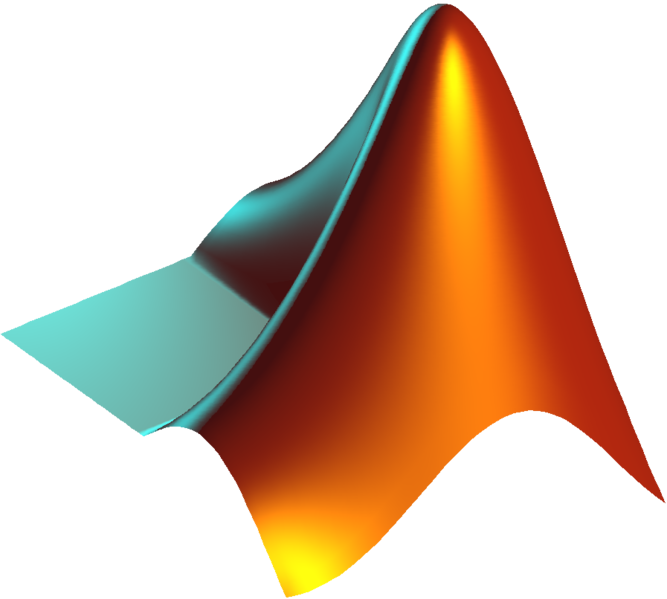
\includegraphics[width=0.1\textwidth]{figures/Matlab_Logo.png}%
    \hspace{0.07\textwidth}%
    
\includegraphics[width=0.1\textwidth]{figures/Python_Logo.png}%
    \hspace{0.07\textwidth}%
    
\includegraphics[width=0.1\textwidth]{figures/C++_Logo.png}%
\end{center}

\end{frame}

\begin{frame}{Goal}
The goal is to provide a usable INTERNODES implementation in Akantu, with attention to a few points:
\begin{itemize}
    \item Robust implementation and extensive tests, to validate the method.
    \item Common architecture for penalty and INTERNODES contact, to make future developments easier and keep the code neatly organized.
    \item Similar Python interface for penalty and INTERNODES contact, to make switching between the methods easy.
\end{itemize}
\end{frame}

\begin{frame}{Extended Python prototype}
\only<1>{
Because three implementations were not enough, we decided to write a fourth one...

\begin{center}
    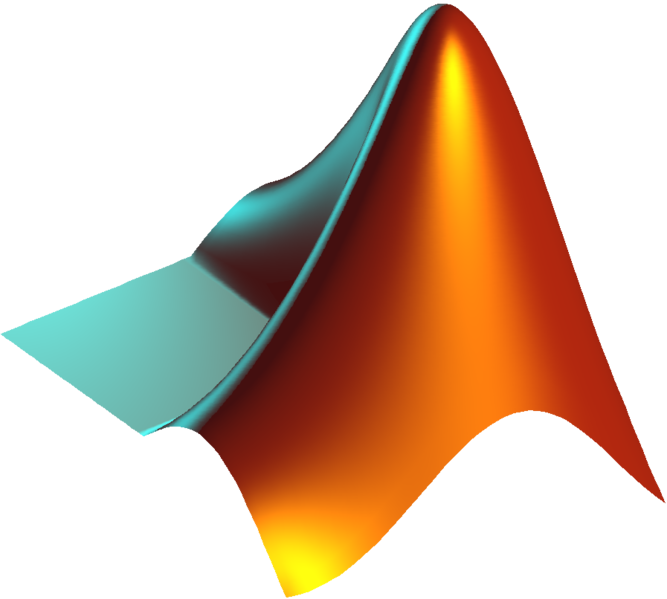
\includegraphics[width=0.1\textwidth]{figures/Matlab_Logo.png}%
    \hspace{0.07\textwidth}%
    
\includegraphics[width=0.1\textwidth]{figures/Python_Logo.png}%
    \hspace{0.07\textwidth}%
    
\includegraphics[width=0.1\textwidth]{figures/C++_Logo.png}%
    \hspace{0.07\textwidth}%
    
\includegraphics[width=0.1\textwidth]{figures/Python_Logo.png}%
\end{center}
}\pause
We refactored Moritz's Python prototype and used it as a testing ground.
\begin{itemize}
    \item Carefully documented every step, with references to the relevant papers.
    \item Convergence check prototyping and first working implementation.
    \item Test case prototyping and first working implementation.
\end{itemize}
All of these improvements were ported to C++.
\end{frame}

\begin{frame}{C++: the convergence check}
\begin{itemize}
    \item Brief reminder of what the convergence check is. % Here I will go back to the Algorithm slide and explain which steps this corresponds to.
    \item Missing in Moritz's C++ implementation, had to be ported from the extended Python prototype.
    \item Normal computations need special attention to work both in 2D and 3D.
    \item The set of active nodes changes at each iteration.
    \begin{itemize}
        \item Number of \(\lambda\) variables changes at each iteration, but we cannot resize the DOFs (degrees of freedom) in Akantu.
        \item Allocate one \(\lambda\) variable for each candidate node.
        \item Add identity submatrix for the inactive variables to preserve numerical stability.
    \end{itemize}
\end{itemize}
\end{frame}

\begin{frame}{Spatial Grids}
For radius parameter search, we need to list the nodes in a (relatively small) circle. How can we do this efficiently?
\begin{itemize}
    \item Option 1: Iterate over each node, check if it's in the circle.
    \item<2-> Option 2: We can build a spatial grid instead, and only check neighboring cells!
    
    \begin{tikzpicture}[x=1.5cm,y=1.5cm]

\draw[ultra thick, mainorange, <->] (2.05, 0.8) -- (2.05, 1.2) node [midway, right, mainorange] {Search radius};

\draw[ultra thick, mainorange] (0, 0.4) to (2, 0.4);
\draw[ultra thick, mainorange] (0, 0.8) to (2, 0.8);
\draw[ultra thick, mainorange] (0, 1.2) to (2, 1.2);
\draw[ultra thick, mainorange] (0, 1.6) to (2, 1.6);
\draw[ultra thick, mainorange] (0.4, 0) to (0.4, 2);
\draw[ultra thick, mainorange] (0.8, 0) to (0.8, 2);
\draw[ultra thick, mainorange] (1.2, 0) to (1.2, 2);
\draw[ultra thick, mainorange] (1.6, 0) to (1.6, 2);

\foreach \Point in {(0.0339222622185466, 0.1306055817982923), (0.4822631927736075, 0.07568029619396875), (0.6217395235277684, 0.13052611394028735), (1.0911779617313586, 0.19234200357957137), (1.397960316238706, 0.1691559350416794), (1.5115355165881585, 0.021049110236548277), (1.998445919730088, 0.11981151946650592), (0.1880938522212483, 0.3683335767044433), (0.4352892496260543, 0.347649164865645), (0.7226758425466797, 0.4774852932061472), (1.0735703596696275, 0.38168067522068017), (1.3401358460486419, 0.31041327519532425), (1.6044424942456275, 0.36280151203536226), (1.9542537495400691, 0.37090273023500614), (0.061717501905212926, 0.6196510072574346), (0.40760664412811065, 0.6392301860052056), (0.692417463619579, 0.6070519612231388), (1.021165961900525, 0.6992857667538572), (1.3135992915856274, 0.7892494720803865), (1.6127743599766386, 0.7264972614838134), (1.815656171324388, 0.7902629906409896), (0.1148422921794715, 1.0158083502601636), (0.37194756504494386, 1.007121429990796), (0.7752675139558673, 0.9821376729765343), (1.066170373974295, 0.960228383473678), (1.2221625250011046, 0.9525681521307292), (1.5257955716089135, 1.0097529607669071), (1.8184264161582184, 0.9396949467196039), (0.10123056797593342, 1.259176968262102), (0.3520669910569994, 1.342293898109578), (0.6008627884950574, 1.2833359674368325), (0.9829243969563952, 1.3667043714738494), (1.261825780411512, 1.3080277551401847), (1.6309532135649931, 1.29629792694812), (1.874748178510847, 1.3353442760746739), (0.16386261752555303, 1.5523582522602364), (0.41945052746827066, 1.69250123506785), (0.7461038517967243, 1.5795071999975459), (1.0653312575171376, 1.5742544469849187), (1.28184713911872, 1.5624128360476075), (1.5314514388189198, 1.6180278667112167), (1.9966939371589871, 1.680842860791491), (0.049176530135727314, 1.9692660883205262), (0.43531961437830174, 1.930637022393717), (0.754398502376105, 1.8696700225624518), (0.9227913486146528, 1.9994183079691976), (1.3929826422576204, 1.8472771500777523), (1.6465596746987368, 1.9257985049681423), (1.8606028797873129, 1.8270948271303513)}{
    \fill[darkblue] \Point  circle[radius=2pt];
}

    %\fill[ultra thick, darkblue!10!white] (-1.5, -3) rectangle (1.5, 0);
    %\fill[ultra thick, darkblue!10!white] (-1.5, 0.25) to (-1.5, 3.25) to (1.5, 3.25) to (1.5, 0.25) to [out=200, in=-20] (-1.5, 0.25);
    %\draw[ultra thick, darkblue] (-1.5, -3) rectangle (1.5, 0);
    %\draw[ultra thick, darkblue] (-1.5, 0.25) to (-1.5, 3.25) to (1.5, 3.25) to (1.5, 0.25) to [out=200, in=-20] (-1.5, 0.25);
    %\node[darkblue] at (0, 1.5) {$\Omega_1$};
    %\node[darkblue] at (0, -1.5) {$\Omega_2$};
    %\draw[ultra thick, darkblue, <-] (0.0, 3.25) to (0.0, 3.75);
    %\draw[ultra thick, darkblue, <-] (1.0, 3.25) to (1.0, 3.75) node[right] {$\mathbf{f}$};
    %\draw[ultra thick, darkblue, <-] (-1.0, 3.25) to (-1.0, 3.75);
    %\onslide<2->{
    %    \draw[ultra thick, red] (0.75, 0.0) to [out=190, in=-10] (-0.75, 0.0);
    %    \draw[ultra thick, red] (0.75, 0.0) to (-0.75, 0.0);
    %    \draw[thick, red, <-] (0, 0.05) to (0.3, 0.5) node[above] {$\Gamma_2$};
    %    \draw[thick, red, <-] (0, -0.15) to (0.3, -0.5) node[below] {$\Gamma_1$};
    %}
\end{tikzpicture}
    \begin{itemize}
        \item Also used by the penalty method, so grid building is shared between the methods via \ci{AbstractContactDetector}.
    \end{itemize}
\end{itemize}
\end{frame}

\begin{frame}{Architecture concerns}
\begin{itemize}
    \item Penalty: separate contact mechanics implementation and solid mechanics implementation, bridged by a \ci{CouplerSolidContact}.
    \begin{itemize}
        \item Dispatches to contained \ci{ContactMechanicsModel}.
        \item Dispatches to contained \ci{SolidMechanicsModel}.
    \end{itemize}
    \item<2-> INTERNODES: the \ci{ContactMechanicsInternodesModel} contains a solid mechanics implementation.
    \begin{itemize}
        \item Contains the INTERNODES contact mechanics code.
        \item Dispatches to contained \ci{SolidMechanicsModel}.
    \end{itemize}
    \item<3-> Refactor INTERNODES to use a coupler too?
    \begin{itemize}
        \item<4-> Problem: Sharing the coupler code is hard due to algorithmic differences. Lots of templates, template specialization and inheritance leading to very complicated code.
        \item<5-> Problem: The standalone contact models are not usable, yet they extend \ci{Model}.
    \end{itemize}
\end{itemize}
\end{frame}

\begin{frame}{Architecture concerns: what we really want}
The goal is to easily swap from one contact mechanics implementation to the other using the Python interface. This can be done without refactoring to a coupler.

\lstinputlisting[language=diff]{listings/run.py.diff}

Current status: works. However, Python uses dynamic typing hence the common interface is not well defined.
\end{frame}

\begin{frame}{Architecture concerns: proposed solution}
We can introduce a well-defined C++ common interface implemented by both \ci{CouplerSolidContact} and \ci{ContactMechanicsInternodesModel}.

\lstinputlisting[language=C++]{listings/solidcontactmodel.hh}
\end{frame}

\begin{frame}{Contact mechanics renames}
\begin{itemize}
    \item For a long time, Akantu only had a single implementation of contact mechanics, which is why its classes use generic names such as \ci{ContactMechanicsModel} or \ci{ContactDetector}.
    \item Now that there is a second contact mechanics implementation, we propose renaming the penalty method classes to more appropriate names.\begin{itemize}
        \item \ci{ContactMechanicsModel} \(\rightarrow\) \ci{ContactMechanicsPenaltyModel}.
        \item \ci{ContactDetector} \(\rightarrow\) \ci{ContactDetectorPenalty}.
        \item \ci{CouplerSolidContact} \(\rightarrow\) \ci{CouplerSolidContactPenalty}.
    \end{itemize}
    \item We intend to carry out these impactful refactors with Nico's approval once INTERNODES is merged.
\end{itemize}
\end{frame}

\begin{frame}{Appendix: Debugging Akantu through Python}
It's possible to step through Akantu C++ code, print variables, etc... even when running it through a Python script. A very handy trick for debugging !
\lstset{escapeinside={(*@}{@*)}}
\lstinputlisting[belowskip=0pt, basicstyle=\tiny, lastline=1]{listings/gdb.txt}%
\pause%
\lstinputlisting[aboveskip=0pt, belowskip=0pt, basicstyle=\tiny, firstline=2, lastline=4]{listings/gdb.txt}%
\pause%
\lstinputlisting[aboveskip=0pt, belowskip=0pt, basicstyle=\tiny, firstline=5, lastline=6]{listings/gdb.txt}%
\pause%
\lstinputlisting[aboveskip=0pt, belowskip=0pt, basicstyle=\tiny, firstline=7, lastline=8]{listings/gdb.txt}%
\pause%
\lstinputlisting[aboveskip=0pt, belowskip=0pt, basicstyle=\tiny, firstline=9, lastline=12]{listings/gdb.txt}%
\pause%
\lstinputlisting[belowskip=0pt, basicstyle=\tiny, firstline=13]{listings/gdb.txt}
\end{frame}

%\begin{frame}{Bibliography}
%\bibliography{biblio.bib}
%\end{frame}






\end{document}